%********************************************%
%*       Generated from PreTeXt source      *%
%*       on 2021-03-19T13:44:26Z       *%
%*   A recent stable commit (2020-08-09):   *%
%* 98f21740783f166a773df4dc83cab5293ab63a4a *%
%*                                          *%
%*         https://pretextbook.org          *%
%*                                          *%
%********************************************%
%% We elect to always write snapshot output into <job>.dep file
\RequirePackage{snapshot}
\documentclass[oneside,10pt,]{book}
%% Custom Preamble Entries, early (use latex.preamble.early)
%% Default LaTeX packages
%%   1.  always employed (or nearly so) for some purpose, or
%%   2.  a stylewriter may assume their presence
\usepackage{geometry}
%% Some aspects of the preamble are conditional,
%% the LaTeX engine is one such determinant
\usepackage{ifthen}
%% etoolbox has a variety of modern conveniences
\usepackage{etoolbox}
\usepackage{ifxetex,ifluatex}
%% Raster graphics inclusion
\usepackage{graphicx}
%% Color support, xcolor package
%% Always loaded, for: add/delete text, author tools
%% Here, since tcolorbox loads tikz, and tikz loads xcolor
\PassOptionsToPackage{usenames,dvipsnames,svgnames,table}{xcolor}
\usepackage{xcolor}
%% begin: defined colors, via xcolor package, for styling
%% end: defined colors, via xcolor package, for styling
%% Colored boxes, and much more, though mostly styling
%% skins library provides "enhanced" skin, employing tikzpicture
%% boxes may be configured as "breakable" or "unbreakable"
%% "raster" controls grids of boxes, aka side-by-side
\usepackage{tcolorbox}
\tcbuselibrary{skins}
\tcbuselibrary{breakable}
\tcbuselibrary{raster}
%% We load some "stock" tcolorbox styles that we use a lot
%% Placement here is provisional, there will be some color work also
%% First, black on white, no border, transparent, but no assumption about titles
\tcbset{ bwminimalstyle/.style={size=minimal, boxrule=-0.3pt, frame empty,
colback=white, colbacktitle=white, coltitle=black, opacityfill=0.0} }
%% Second, bold title, run-in to text/paragraph/heading
%% Space afterwards will be controlled by environment,
%% independent of constructions of the tcb title
%% Places \blocktitlefont onto many block titles
\tcbset{ runintitlestyle/.style={fonttitle=\blocktitlefont\upshape\bfseries, attach title to upper} }
%% Spacing prior to each exercise, anywhere
\tcbset{ exercisespacingstyle/.style={before skip={1.5ex plus 0.5ex}} }
%% Spacing prior to each block
\tcbset{ blockspacingstyle/.style={before skip={2.0ex plus 0.5ex}} }
%% xparse allows the construction of more robust commands,
%% this is a necessity for isolating styling and behavior
%% The tcolorbox library of the same name loads the base library
\tcbuselibrary{xparse}
%% Hyperref should be here, but likes to be loaded late
%%
%% Inline math delimiters, \(, \), need to be robust
%% 2016-01-31:  latexrelease.sty  supersedes  fixltx2e.sty
%% If  latexrelease.sty  exists, bugfix is in kernel
%% If not, bugfix is in  fixltx2e.sty
%% See:  https://tug.org/TUGboat/tb36-3/tb114ltnews22.pdf
%% and read "Fewer fragile commands" in distribution's  latexchanges.pdf
\IfFileExists{latexrelease.sty}{}{\usepackage{fixltx2e}}
%% shorter subnumbers in some side-by-side require manipulations
\usepackage{xstring}
%% Footnote counters and part/chapter counters are manipulated
%% April 2018:  chngcntr  commands now integrated into the kernel,
%% but circa 2018/2019 the package would still try to redefine them,
%% so we need to do the work of loading conditionally for old kernels.
%% From version 1.1a,  chngcntr  should detect defintions made by LaTeX kernel.
\ifdefined\counterwithin
\else
    \usepackage{chngcntr}
\fi
%% Text height identically 9 inches, text width varies on point size
%% See Bringhurst 2.1.1 on measure for recommendations
%% 75 characters per line (count spaces, punctuation) is target
%% which is the upper limit of Bringhurst's recommendations
\geometry{letterpaper,total={340pt,9.0in}}
%% Custom Page Layout Adjustments (use latex.geometry)
%% This LaTeX file may be compiled with pdflatex, xelatex, or lualatex executables
%% LuaTeX is not explicitly supported, but we do accept additions from knowledgeable users
%% The conditional below provides  pdflatex  specific configuration last
%% begin: engine-specific capabilities
\ifthenelse{\boolean{xetex} \or \boolean{luatex}}{%
%% begin: xelatex and lualatex-specific default configuration
\ifxetex\usepackage{xltxtra}\fi
%% realscripts is the only part of xltxtra relevant to lualatex 
\ifluatex\usepackage{realscripts}\fi
%% end:   xelatex and lualatex-specific default configuration
}{
%% begin: pdflatex-specific default configuration
%% We assume a PreTeXt XML source file may have Unicode characters
%% and so we ask LaTeX to parse a UTF-8 encoded file
%% This may work well for accented characters in Western language,
%% but not with Greek, Asian languages, etc.
%% When this is not good enough, switch to the  xelatex  engine
%% where Unicode is better supported (encouraged, even)
\usepackage[utf8]{inputenc}
%% end: pdflatex-specific default configuration
}
%% end:   engine-specific capabilities
%%
%% Fonts.  Conditional on LaTex engine employed.
%% Default Text Font: The Latin Modern fonts are
%% "enhanced versions of the [original TeX] Computer Modern fonts."
%% We use them as the default text font for PreTeXt output.
%% Default Monospace font: Inconsolata (aka zi4)
%% Sponsored by TUG: http://levien.com/type/myfonts/inconsolata.html
%% Loaded for documents with intentional objects requiring monospace
%% See package documentation for excellent instructions
%% fontspec will work universally if we use filename to locate OTF files
%% Loads the "upquote" package as needed, so we don't have to
%% Upright quotes might come from the  textcomp  package, which we also use
%% We employ the shapely \ell to match Google Font version
%% pdflatex: "varl" package option produces shapely \ell
%% pdflatex: "var0" package option produces plain zero (not used)
%% pdflatex: "varqu" package option produces best upright quotes
%% xelatex,lualatex: add OTF StylisticSet 1 for shapely \ell
%% xelatex,lualatex: add OTF StylisticSet 2 for plain zero (not used)
%% xelatex,lualatex: add OTF StylisticSet 3 for upright quotes
%%
%% Automatic Font Control
%% Portions of a document, are, or may, be affected by defined commands
%% These are perhaps more flexible when using  xelatex  rather than  pdflatex
%% The following definitions are meant to be re-defined in a style, using \renewcommand
%% They are scoped when employed (in a TeX group), and so should not be defined with an argument
\newcommand{\divisionfont}{\relax}
\newcommand{\blocktitlefont}{\relax}
\newcommand{\contentsfont}{\relax}
\newcommand{\pagefont}{\relax}
\newcommand{\tabularfont}{\relax}
\newcommand{\xreffont}{\relax}
\newcommand{\titlepagefont}{\relax}
%%
\ifthenelse{\boolean{xetex} \or \boolean{luatex}}{%
%% begin: font setup and configuration for use with xelatex
%% Generally, xelatex is necessary for non-Western fonts
%% fontspec package provides extensive control of system fonts,
%% meaning *.otf (OpenType), and apparently *.ttf (TrueType)
%% that live *outside* your TeX/MF tree, and are controlled by your *system*
%% (it is possible that a TeX distribution will place fonts in a system location)
%%
%% The fontspec package is the best vehicle for using different fonts in  xelatex
%% So we load it always, no matter what a publisher or style might want
%%
\usepackage{fontspec}
%%
%% begin: xelatex main font ("font-xelatex-main" template)
%% Latin Modern Roman is the default font for xelatex and so is loaded with a TU encoding
%% *in the format* so we can't touch it, only perhaps adjust it later
%% in one of two ways (then known by NFSS names such as "lmr")
%% (1) via NFSS with font family names such as "lmr" and "lmss"
%% (2) via fontspec with commands like \setmainfont{Latin Modern Roman}
%% The latter requires the font to be known at the system-level by its font name,
%% but will give access to OTF font features through optional arguments
%% https://tex.stackexchange.com/questions/470008/
%% where-and-how-does-fontspec-sty-specify-the-default-font-latin-modern-roman
%% http://tex.stackexchange.com/questions/115321
%% /how-to-optimize-latin-modern-font-with-xelatex
%%
%% end:   xelatex main font ("font-xelatex-main" template)
%% begin: xelatex mono font ("font-xelatex-mono" template)
%% (conditional on non-trivial uses being present in source)
\IfFontExistsTF{Inconsolatazi4-Regular.otf}{}{\GenericError{}{The font "Inconsolatazi4-Regular.otf" requested by PreTeXt output is not available.  Either a file cannot be located in default locations via a filename, or a font is not known by its name as part of your system.}{Consult the PreTeXt Guide for help with LaTeX fonts.}{}}
\IfFontExistsTF{Inconsolatazi4-Bold.otf}{}{\GenericError{}{The font "Inconsolatazi4-Bold.otf" requested by PreTeXt output is not available.  Either a file cannot be located in default locations via a filename, or a font is not known by its name as part of your system.}{Consult the PreTeXt Guide for help with LaTeX fonts.}{}}
\usepackage{zi4}
\setmonofont[BoldFont=Inconsolatazi4-Bold.otf,StylisticSet={1,3}]{Inconsolatazi4-Regular.otf}
%% end:   xelatex mono font ("font-xelatex-mono" template)
%% begin: xelatex font adjustments ("font-xelatex-style" template)
%% end:   xelatex font adjustments ("font-xelatex-style" template)
%%
%% Extensive support for other languages
\usepackage{polyglossia}
%% Set main/default language based on pretext/@xml:lang value
%% document language code is "en-US", US English
%% usmax variant has extra hypenation
\setmainlanguage[variant=usmax]{english}
%% Enable secondary languages based on discovery of @xml:lang values
%% Enable fonts/scripts based on discovery of @xml:lang values
%% Western languages should be ably covered by Latin Modern Roman
%% end:   font setup and configuration for use with xelatex
}{%
%% begin: font setup and configuration for use with pdflatex
%% begin: pdflatex main font ("font-pdflatex-main" template)
\usepackage{lmodern}
\usepackage[T1]{fontenc}
%% end:   pdflatex main font ("font-pdflatex-main" template)
%% begin: pdflatex mono font ("font-pdflatex-mono" template)
%% (conditional on non-trivial uses being present in source)
\usepackage[varqu,varl]{inconsolata}
%% end:   pdflatex mono font ("font-pdflatex-mono" template)
%% begin: pdflatex font adjustments ("font-pdflatex-style" template)
%% end:   pdflatex font adjustments ("font-pdflatex-style" template)
%% end:   font setup and configuration for use with pdflatex
}
%% Micromanage spacing, etc.  The named "microtype-options"
%% template may be employed to fine-tune package behavior
\usepackage{microtype}
%% Symbols, align environment, commutative diagrams, bracket-matrix
\usepackage{amsmath}
\usepackage{amscd}
\usepackage{amssymb}
%% allow page breaks within display mathematics anywhere
%% level 4 is maximally permissive
%% this is exactly the opposite of AMSmath package philosophy
%% there are per-display, and per-equation options to control this
%% split, aligned, gathered, and alignedat are not affected
\allowdisplaybreaks[4]
%% allow more columns to a matrix
%% can make this even bigger by overriding with  latex.preamble.late  processing option
\setcounter{MaxMatrixCols}{30}
%%
%%
%% Division Titles, and Page Headers/Footers
%% titlesec package, loading "titleps" package cooperatively
%% See code comments about the necessity and purpose of "explicit" option.
%% The "newparttoc" option causes a consistent entry for parts in the ToC 
%% file, but it is only effective if there is a \titleformat for \part.
%% "pagestyles" loads the  titleps  package cooperatively.
\usepackage[explicit, newparttoc, pagestyles]{titlesec}
%% The companion titletoc package for the ToC.
\usepackage{titletoc}
%% Fixes a bug with transition from chapters to appendices in a "book"
%% See generating XSL code for more details about necessity
\newtitlemark{\chaptertitlename}
%% begin: customizations of page styles via the modal "titleps-style" template
%% Designed to use commands from the LaTeX "titleps" package
%% Plain pages should have the same font for page numbers
\renewpagestyle{plain}{%
\setfoot{}{\pagefont\thepage}{}%
}%
%% Single pages as in default LaTeX
\renewpagestyle{headings}{%
\sethead{\pagefont\slshape\MakeUppercase{\ifthechapter{\chaptertitlename\space\thechapter.\space}{}\chaptertitle}}{}{\pagefont\thepage}%
}%
\pagestyle{headings}
%% end: customizations of page styles via the modal "titleps-style" template
%%
%% Create globally-available macros to be provided for style writers
%% These are redefined for each occurence of each division
\newcommand{\divisionnameptx}{\relax}%
\newcommand{\titleptx}{\relax}%
\newcommand{\subtitleptx}{\relax}%
\newcommand{\shortitleptx}{\relax}%
\newcommand{\authorsptx}{\relax}%
\newcommand{\epigraphptx}{\relax}%
%% Create environments for possible occurences of each division
%% Environment for a PTX "chapter" at the level of a LaTeX "chapter"
\NewDocumentEnvironment{chapterptx}{mmmmmm}
{%
\renewcommand{\divisionnameptx}{Chapter}%
\renewcommand{\titleptx}{#1}%
\renewcommand{\subtitleptx}{#2}%
\renewcommand{\shortitleptx}{#3}%
\renewcommand{\authorsptx}{#4}%
\renewcommand{\epigraphptx}{#5}%
\chapter[{#3}]{#1}%
\label{#6}%
}{}%
%% Environment for a PTX "section" at the level of a LaTeX "section"
\NewDocumentEnvironment{sectionptx}{mmmmmm}
{%
\renewcommand{\divisionnameptx}{Section}%
\renewcommand{\titleptx}{#1}%
\renewcommand{\subtitleptx}{#2}%
\renewcommand{\shortitleptx}{#3}%
\renewcommand{\authorsptx}{#4}%
\renewcommand{\epigraphptx}{#5}%
\section[{#3}]{#1}%
\label{#6}%
}{}%
%% Environment for a PTX "subsection" at the level of a LaTeX "subsection"
\NewDocumentEnvironment{subsectionptx}{mmmmmm}
{%
\renewcommand{\divisionnameptx}{Subsection}%
\renewcommand{\titleptx}{#1}%
\renewcommand{\subtitleptx}{#2}%
\renewcommand{\shortitleptx}{#3}%
\renewcommand{\authorsptx}{#4}%
\renewcommand{\epigraphptx}{#5}%
\subsection[{#3}]{#1}%
\label{#6}%
}{}%
%% Environment for a PTX "exercises" at the level of a LaTeX "section"
\NewDocumentEnvironment{exercises-section}{mmmmmm}
{%
\renewcommand{\divisionnameptx}{Exercises}%
\renewcommand{\titleptx}{#1}%
\renewcommand{\subtitleptx}{#2}%
\renewcommand{\shortitleptx}{#3}%
\renewcommand{\authorsptx}{#4}%
\renewcommand{\epigraphptx}{#5}%
\section[{#3}]{#1}%
\label{#6}%
}{}%
%% Environment for a PTX "exercises" at the level of a LaTeX "section"
\NewDocumentEnvironment{exercises-section-numberless}{mmmmmm}
{%
\renewcommand{\divisionnameptx}{Exercises}%
\renewcommand{\titleptx}{#1}%
\renewcommand{\subtitleptx}{#2}%
\renewcommand{\shortitleptx}{#3}%
\renewcommand{\authorsptx}{#4}%
\renewcommand{\epigraphptx}{#5}%
\section*{#1}%
\addcontentsline{toc}{section}{#3}
\label{#6}%
}{}%
%%
%% Styles for six traditional LaTeX divisions
\titleformat{\part}[display]
{\divisionfont\Huge\bfseries\centering}{\divisionnameptx\space\thepart}{30pt}{\Huge#1}
[{\Large\centering\authorsptx}]
\titleformat{\chapter}[display]
{\divisionfont\huge\bfseries}{\divisionnameptx\space\thechapter}{20pt}{\Huge#1}
[{\Large\authorsptx}]
\titleformat{name=\chapter,numberless}[display]
{\divisionfont\huge\bfseries}{}{0pt}{#1}
[{\Large\authorsptx}]
\titlespacing*{\chapter}{0pt}{50pt}{40pt}
\titleformat{\section}[hang]
{\divisionfont\Large\bfseries}{\thesection}{1ex}{#1}
[{\large\authorsptx}]
\titleformat{name=\section,numberless}[block]
{\divisionfont\Large\bfseries}{}{0pt}{#1}
[{\large\authorsptx}]
\titlespacing*{\section}{0pt}{3.5ex plus 1ex minus .2ex}{2.3ex plus .2ex}
\titleformat{\subsection}[hang]
{\divisionfont\large\bfseries}{\thesubsection}{1ex}{#1}
[{\normalsize\authorsptx}]
\titleformat{name=\subsection,numberless}[block]
{\divisionfont\large\bfseries}{}{0pt}{#1}
[{\normalsize\authorsptx}]
\titlespacing*{\subsection}{0pt}{3.25ex plus 1ex minus .2ex}{1.5ex plus .2ex}
\titleformat{\subsubsection}[hang]
{\divisionfont\normalsize\bfseries}{\thesubsubsection}{1em}{#1}
[{\small\authorsptx}]
\titleformat{name=\subsubsection,numberless}[block]
{\divisionfont\normalsize\bfseries}{}{0pt}{#1}
[{\normalsize\authorsptx}]
\titlespacing*{\subsubsection}{0pt}{3.25ex plus 1ex minus .2ex}{1.5ex plus .2ex}
\titleformat{\paragraph}[hang]
{\divisionfont\normalsize\bfseries}{\theparagraph}{1em}{#1}
[{\small\authorsptx}]
\titleformat{name=\paragraph,numberless}[block]
{\divisionfont\normalsize\bfseries}{}{0pt}{#1}
[{\normalsize\authorsptx}]
\titlespacing*{\paragraph}{0pt}{3.25ex plus 1ex minus .2ex}{1.5em}
%%
%% Styles for five traditional LaTeX divisions
\titlecontents{part}%
[0pt]{\contentsmargin{0em}\addvspace{1pc}\contentsfont\bfseries}%
{\Large\thecontentslabel\enspace}{\Large}%
{}%
[\addvspace{.5pc}]%
\titlecontents{chapter}%
[0pt]{\contentsmargin{0em}\addvspace{1pc}\contentsfont\bfseries}%
{\large\thecontentslabel\enspace}{\large}%
{\hfill\bfseries\thecontentspage}%
[\addvspace{.5pc}]%
\dottedcontents{section}[3.8em]{\contentsfont}{2.3em}{1pc}%
\dottedcontents{subsection}[6.1em]{\contentsfont}{3.2em}{1pc}%
\dottedcontents{subsubsection}[9.3em]{\contentsfont}{4.3em}{1pc}%
%%
%% Begin: Semantic Macros
%% To preserve meaning in a LaTeX file
%%
%% \mono macro for content of "c", "cd", "tag", etc elements
%% Also used automatically in other constructions
%% Simply an alias for \texttt
%% Always defined, even if there is no need, or if a specific tt font is not loaded
\newcommand{\mono}[1]{\texttt{#1}}
%%
%% Following semantic macros are only defined here if their
%% use is required only in this specific document
%%
%% Used for warnings, typically bold and italic
\newcommand{\alert}[1]{\textbf{\textit{#1}}}
%% Used for inline definitions of terms
\newcommand{\terminology}[1]{\textbf{#1}}
%% End: Semantic Macros
%% Division Numbering: Chapters, Sections, Subsections, etc
%% Division numbers may be turned off at some level ("depth")
%% A section *always* has depth 1, contrary to us counting from the document root
%% The latex default is 3.  If a larger number is present here, then
%% removing this command may make some cross-references ambiguous
%% The precursor variable $numbering-maxlevel is checked for consistency in the common XSL file
\setcounter{secnumdepth}{3}
%%
%% AMS "proof" environment is no longer used, but we leave previously
%% implemented \qedhere in place, should the LaTeX be recycled
\newcommand{\qedhere}{\relax}
%%
%% A faux tcolorbox whose only purpose is to provide common numbering
%% facilities for most blocks (possibly not projects, 2D displays)
%% Controlled by  numbering.theorems.level  processing parameter
\newtcolorbox[auto counter, number within=section]{block}{}
%%
%% This document is set to number PROJECT-LIKE on a separate numbering scheme
%% So, a faux tcolorbox whose only purpose is to provide this numbering
%% Controlled by  numbering.projects.level  processing parameter
\newtcolorbox[auto counter, number within=section]{project-distinct}{}
%% A faux tcolorbox whose only purpose is to provide common numbering
%% facilities for 2D displays which are subnumbered as part of a "sidebyside"
\makeatletter
\newtcolorbox[auto counter, number within=tcb@cnt@block, number freestyle={\noexpand\thetcb@cnt@block(\noexpand\alph{\tcbcounter})}]{subdisplay}{}
\makeatother
%%
%% tcolorbox, with styles, for THEOREM-LIKE
%%
%% lemma: fairly simple numbered block/structure
\tcbset{ lemmastyle/.style={bwminimalstyle, runintitlestyle, blockspacingstyle, after title={\space}, } }
\newtcolorbox[use counter from=block]{lemma}[3]{title={{Lemma~\thetcbcounter\notblank{#1#2}{\space}{}\notblank{#1}{\space#1}{}\notblank{#2}{\space(#2)}{}}}, phantomlabel={#3}, breakable, parbox=false, after={\par}, fontupper=\itshape, lemmastyle, }
%% theorem: fairly simple numbered block/structure
\tcbset{ theoremstyle/.style={bwminimalstyle, runintitlestyle, blockspacingstyle, after title={\space}, } }
\newtcolorbox[use counter from=block]{theorem}[3]{title={{Theorem~\thetcbcounter\notblank{#1#2}{\space}{}\notblank{#1}{\space#1}{}\notblank{#2}{\space(#2)}{}}}, phantomlabel={#3}, breakable, parbox=false, after={\par}, fontupper=\itshape, theoremstyle, }
%% algorithm: fairly simple numbered block/structure
\tcbset{ algorithmstyle/.style={bwminimalstyle, runintitlestyle, blockspacingstyle, after title={\space}, } }
\newtcolorbox[use counter from=block]{algorithm}[3]{title={{Algorithm~\thetcbcounter\notblank{#1#2}{\space}{}\notblank{#1}{\space#1}{}\notblank{#2}{\space(#2)}{}}}, phantomlabel={#3}, breakable, parbox=false, after={\par}, fontupper=\itshape, algorithmstyle, }
%% proposition: fairly simple numbered block/structure
\tcbset{ propositionstyle/.style={bwminimalstyle, runintitlestyle, blockspacingstyle, after title={\space}, } }
\newtcolorbox[use counter from=block]{proposition}[3]{title={{Proposition~\thetcbcounter\notblank{#1#2}{\space}{}\notblank{#1}{\space#1}{}\notblank{#2}{\space(#2)}{}}}, phantomlabel={#3}, breakable, parbox=false, after={\par}, fontupper=\itshape, propositionstyle, }
%%
%% tcolorbox, with styles, for DEFINITION-LIKE
%%
%% definition: fairly simple numbered block/structure
\tcbset{ definitionstyle/.style={bwminimalstyle, runintitlestyle, blockspacingstyle, after title={\space}, after upper={\space\space\hspace*{\stretch{1}}\(\lozenge\)}, } }
\newtcolorbox[use counter from=block]{definition}[2]{title={{Definition~\thetcbcounter\notblank{#1}{\space\space#1}{}}}, phantomlabel={#2}, breakable, parbox=false, after={\par}, definitionstyle, }
%%
%% tcolorbox, with styles, for REMARK-LIKE
%%
%% remark: fairly simple numbered block/structure
\tcbset{ remarkstyle/.style={bwminimalstyle, runintitlestyle, blockspacingstyle, after title={\space}, } }
\newtcolorbox[use counter from=block]{remark}[2]{title={{Remark~\thetcbcounter\notblank{#1}{\space\space#1}{}}}, phantomlabel={#2}, breakable, parbox=false, after={\par}, remarkstyle, }
%%
%% tcolorbox, with styles, for EXAMPLE-LIKE
%%
%% example: fairly simple numbered block/structure
\tcbset{ examplestyle/.style={bwminimalstyle, runintitlestyle, blockspacingstyle, after title={\space}, after upper={\space\space\hspace*{\stretch{1}}\(\square\)}, } }
\newtcolorbox[use counter from=block]{example}[2]{title={{Example~\thetcbcounter\notblank{#1}{\space\space#1}{}}}, phantomlabel={#2}, breakable, parbox=false, after={\par}, examplestyle, }
%% problem: fairly simple numbered block/structure
\tcbset{ problemstyle/.style={bwminimalstyle, runintitlestyle, blockspacingstyle, after title={\space}, after upper={\space\space\hspace*{\stretch{1}}\(\square\)}, } }
\newtcolorbox[use counter from=block]{problem}[2]{title={{Problem~\thetcbcounter\notblank{#1}{\space\space#1}{}}}, phantomlabel={#2}, breakable, parbox=false, after={\par}, problemstyle, }
%%
%% tcolorbox, with styles, for inline exercises
%%
%% inlineexercise: fairly simple numbered block/structure
\tcbset{ inlineexercisestyle/.style={bwminimalstyle, runintitlestyle, blockspacingstyle, after title={\space}, } }
\newtcolorbox[use counter from=block]{inlineexercise}[2]{title={{Checkpoint~\thetcbcounter\notblank{#1}{\space\space#1}{}}}, phantomlabel={#2}, breakable, parbox=false, after={\par}, inlineexercisestyle, }
%%
%% tcolorbox, with styles, for FIGURE-LIKE
%%
%% figureptx: 2-D display structure
\tcbset{ figureptxstyle/.style={bwminimalstyle, middle=1ex, blockspacingstyle, fontlower=\blocktitlefont} }
\newtcolorbox[use counter from=block]{figureptx}[3]{lower separated=false, before lower={{\textbf{Figure~\thetcbcounter}\space#1}}, phantomlabel={#2}, unbreakable, parbox=false, figureptxstyle, }
%% tableptx: 2-D display structure
\tcbset{ tableptxstyle/.style={bwminimalstyle, middle=1ex, blockspacingstyle, coltitle=black, bottomtitle=2ex, titlerule=-0.3pt, fonttitle=\blocktitlefont} }
\newtcolorbox[use counter from=block]{tableptx}[3]{title={{\textbf{Table~\thetcbcounter}\space#1}}, phantomlabel={#2}, unbreakable, parbox=false, tableptxstyle, }
%%
%% xparse environments for introductions and conclusions of divisions
%%
%% introduction: in a structured division
\NewDocumentEnvironment{introduction}{m}
{\notblank{#1}{\noindent\textbf{#1}\space}{}}{\par\medskip}
%%
%% tcolorbox, with styles, for miscellaneous environments
%%
%% proof: title is a replacement
\tcbset{ proofstyle/.style={bwminimalstyle, fonttitle=\blocktitlefont\itshape, attach title to upper, after title={\space}, after upper={\space\space\hspace*{\stretch{1}}\(\blacksquare\)},
} }
\newtcolorbox{proof}[2]{title={\notblank{#1}{#1}{Proof.}}, phantom={\hypertarget{#2}{}}, breakable, parbox=false, after={\par}, proofstyle }
%% paragraphs: the terminal, pseudo-division
%% We use the lowest LaTeX traditional division
\titleformat{\subparagraph}[runin]{\normalfont\normalsize\bfseries}{\thesubparagraph}{1em}{#1}
\titlespacing*{\subparagraph}{0pt}{3.25ex plus 1ex minus .2ex}{1em}
\NewDocumentEnvironment{paragraphs}{mm}
{\subparagraph*{#1}\hypertarget{#2}{}}{}
%% Divisional exercises (and worksheet) as LaTeX environments
%% Third argument is option for extra workspace in worksheets
%% Hanging indent occupies a 5ex width slot prior to left margin
%% Experimentally this seems just barely sufficient for a bold "888."
%% Division exercises, not in exercise group
\tcbset{ divisionexercisestyle/.style={bwminimalstyle, runintitlestyle, exercisespacingstyle, left=5ex, breakable, parbox=false } }
\newtcolorbox{divisionexercise}[4]{divisionexercisestyle, before title={\hspace{-5ex}\makebox[5ex][l]{#1.}}, title={\notblank{#2}{#2\space}{}}, phantom={\hypertarget{#4}{}}, after={\notblank{#3}{\newline\rule{\workspacestrutwidth}{#3\textheight}\newline}{}}}
%% Localize LaTeX supplied names (possibly none)
\renewcommand*{\chaptername}{Chapter}
%% Equation Numbering
%% Controlled by  numbering.equations.level  processing parameter
%% No adjustment here implies document-wide numbering
\numberwithin{equation}{section}
%% "tcolorbox" environment for a single image, occupying entire \linewidth
%% arguments are left-margin, width, right-margin, as multiples of
%% \linewidth, and are guaranteed to be positive and sum to 1.0
\tcbset{ imagestyle/.style={bwminimalstyle} }
\NewTColorBox{image}{mmm}{imagestyle,left skip=#1\linewidth,width=#2\linewidth}
%% For improved tables
\usepackage{array}
%% Some extra height on each row is desirable, especially with horizontal rules
%% Increment determined experimentally
\setlength{\extrarowheight}{0.2ex}
%% Define variable thickness horizontal rules, full and partial
%% Thicknesses are 0.03, 0.05, 0.08 in the  booktabs  package
\newcommand{\hrulethin}  {\noalign{\hrule height 0.04em}}
\newcommand{\hrulemedium}{\noalign{\hrule height 0.07em}}
\newcommand{\hrulethick} {\noalign{\hrule height 0.11em}}
%% We preserve a copy of the \setlength package before other
%% packages (extpfeil) get a chance to load packages that redefine it
\let\oldsetlength\setlength
\newlength{\Oldarrayrulewidth}
\newcommand{\crulethin}[1]%
{\noalign{\global\oldsetlength{\Oldarrayrulewidth}{\arrayrulewidth}}%
\noalign{\global\oldsetlength{\arrayrulewidth}{0.04em}}\cline{#1}%
\noalign{\global\oldsetlength{\arrayrulewidth}{\Oldarrayrulewidth}}}%
\newcommand{\crulemedium}[1]%
{\noalign{\global\oldsetlength{\Oldarrayrulewidth}{\arrayrulewidth}}%
\noalign{\global\oldsetlength{\arrayrulewidth}{0.07em}}\cline{#1}%
\noalign{\global\oldsetlength{\arrayrulewidth}{\Oldarrayrulewidth}}}
\newcommand{\crulethick}[1]%
{\noalign{\global\oldsetlength{\Oldarrayrulewidth}{\arrayrulewidth}}%
\noalign{\global\oldsetlength{\arrayrulewidth}{0.11em}}\cline{#1}%
\noalign{\global\oldsetlength{\arrayrulewidth}{\Oldarrayrulewidth}}}
%% Single letter column specifiers defined via array package
\newcolumntype{A}{!{\vrule width 0.04em}}
\newcolumntype{B}{!{\vrule width 0.07em}}
\newcolumntype{C}{!{\vrule width 0.11em}}
%% tcolorbox to place tabular outside of a sidebyside
\tcbset{ tabularboxstyle/.style={bwminimalstyle,} }
\newtcolorbox{tabularbox}[3]{tabularboxstyle, left skip=#1\linewidth, width=#2\linewidth,}
%% Footnote Numbering
%% Specified by numbering.footnotes.level
%% Undo counter reset by chapter for a book
\counterwithout{footnote}{chapter}
\counterwithin*{footnote}{section}
%% QR Code Support
%% Videos and other interactives
\usepackage{qrcode}
\newlength{\qrsize}
\newlength{\previewwidth}
%% tcolorbox styles for interactive previews
%% changing size= and/or colback can aid in debugging
\tcbset{ previewstyle/.style={bwminimalstyle, halign=center} }
\tcbset{ qrstyle/.style={bwminimalstyle, hbox} }
\tcbset{ captionstyle/.style={bwminimalstyle, left=1em, width=\linewidth} }
%% Generic red play button (from SVG)
%% tikz package should be loaded by now
\definecolor{playred}{RGB}{230,33,23}
\newcommand{\genericpreview}{
        \begin{tikzpicture}[y=0.80pt, x=0.80pt, yscale=-1.000000, xscale=1.000000, inner sep=0pt, outer sep=0pt]
        \path[fill=playred] (94.9800,28.8400) .. controls (94.9800,28.8400) and
        (94.0400,22.2400) .. (91.1700,19.3400) .. controls (87.5300,15.5300) and
        (83.4500,15.5100) .. (81.5800,15.2900) .. controls (68.1800,14.3200) and
        (48.0600,14.4400) .. (48.0600,14.4400) .. controls (48.0600,14.4400) and
        (27.9400,14.3200) .. (14.5400,15.2900) .. controls (12.6700,15.5100) and
        (8.5900,15.5300) .. (4.9500,19.3400) .. controls (2.0800,22.2400) and
        (1.1400,28.8400) .. (1.1400,28.8400) .. controls (1.1400,28.8400) and
        (0.1800,36.5800) .. (0.0000,44.3300) -- (0.0000,51.5900) .. controls
        (0.1800,59.3400) and (1.1400,67.0800) .. (1.1400,67.0800) .. controls
        (1.1400,67.0800) and (2.0700,73.6800) .. (4.9500,76.5800) .. controls
        (8.5900,80.3900) and (13.3800,80.2700) .. (15.5100,80.6700) .. controls
        (23.0400,81.3900) and (47.2100,81.5600) .. (48.0500,81.5700) .. controls
        (48.0600,81.5700) and (68.1900,81.6000) .. (81.5900,80.6300) .. controls
        (83.4600,80.4100) and (87.5400,80.3900) .. (91.1800,76.5800) .. controls
        (94.0500,73.6800) and (94.9900,67.0800) .. (94.9900,67.0800) .. controls
        (94.9900,67.0800) and (95.9500,59.3300) .. (96.0100,51.5900) --
        (96.0100,44.3300) .. controls (95.9400,36.5800) and (94.9800,28.8400) ..
        (94.9800,28.8400) -- cycle(38.2800,61.4100) -- (38.2800,34.4100) --
        (64.0200,47.9100) -- (38.2800,61.4100) -- cycle;
        \end{tikzpicture}
        }
%% Program listing support: for listings, programs, consoles, and Sage code
\ifthenelse{\boolean{xetex} \or \boolean{luatex}}%
  {\tcbuselibrary{listings}}%
  {\tcbuselibrary{listingsutf8}}%
%% We define the listings font style to be the default "ttfamily"
%% To fix hyphens/dashes rendered in PDF as fancy minus signs by listing
%% http://tex.stackexchange.com/questions/33185/listings-package-changes-hyphens-to-minus-signs
\makeatletter
\lst@CCPutMacro\lst@ProcessOther {"2D}{\lst@ttfamily{-{}}{-{}}}
\@empty\z@\@empty
\makeatother
%% We define a null language, free of any formatting or style
%% for use when a language is not supported, or pseudo-code, or consoles
%% Not necessary for Sage code, so in limited cases included unnecessarily
\lstdefinelanguage{none}{identifierstyle=,commentstyle=,stringstyle=,keywordstyle=}
\ifthenelse{\boolean{xetex}}{}{%
%% begin: pdflatex-specific listings configuration
%% translate U+0080 - U+00F0 to their textmode LaTeX equivalents
%% Data originally from https://www.w3.org/Math/characters/unicode.xml, 2016-07-23
%% Lines marked in XSL with "$" were converted from mathmode to textmode
\lstset{extendedchars=true}
\lstset{literate={ }{{~}}{1}{¡}{{\textexclamdown }}{1}{¢}{{\textcent }}{1}{£}{{\textsterling }}{1}{¤}{{\textcurrency }}{1}{¥}{{\textyen }}{1}{¦}{{\textbrokenbar }}{1}{§}{{\textsection }}{1}{¨}{{\textasciidieresis }}{1}{©}{{\textcopyright }}{1}{ª}{{\textordfeminine }}{1}{«}{{\guillemotleft }}{1}{¬}{{\textlnot }}{1}{­}{{\-}}{1}{®}{{\textregistered }}{1}{¯}{{\textasciimacron }}{1}{°}{{\textdegree }}{1}{±}{{\textpm }}{1}{²}{{\texttwosuperior }}{1}{³}{{\textthreesuperior }}{1}{´}{{\textasciiacute }}{1}{µ}{{\textmu }}{1}{¶}{{\textparagraph }}{1}{·}{{\textperiodcentered }}{1}{¸}{{\c{}}}{1}{¹}{{\textonesuperior }}{1}{º}{{\textordmasculine }}{1}{»}{{\guillemotright }}{1}{¼}{{\textonequarter }}{1}{½}{{\textonehalf }}{1}{¾}{{\textthreequarters }}{1}{¿}{{\textquestiondown }}{1}{À}{{\`{A}}}{1}{Á}{{\'{A}}}{1}{Â}{{\^{A}}}{1}{Ã}{{\~{A}}}{1}{Ä}{{\"{A}}}{1}{Å}{{\AA }}{1}{Æ}{{\AE }}{1}{Ç}{{\c{C}}}{1}{È}{{\`{E}}}{1}{É}{{\'{E}}}{1}{Ê}{{\^{E}}}{1}{Ë}{{\"{E}}}{1}{Ì}{{\`{I}}}{1}{Í}{{\'{I}}}{1}{Î}{{\^{I}}}{1}{Ï}{{\"{I}}}{1}{Ð}{{\DH }}{1}{Ñ}{{\~{N}}}{1}{Ò}{{\`{O}}}{1}{Ó}{{\'{O}}}{1}{Ô}{{\^{O}}}{1}{Õ}{{\~{O}}}{1}{Ö}{{\"{O}}}{1}{×}{{\texttimes }}{1}{Ø}{{\O }}{1}{Ù}{{\`{U}}}{1}{Ú}{{\'{U}}}{1}{Û}{{\^{U}}}{1}{Ü}{{\"{U}}}{1}{Ý}{{\'{Y}}}{1}{Þ}{{\TH }}{1}{ß}{{\ss }}{1}{à}{{\`{a}}}{1}{á}{{\'{a}}}{1}{â}{{\^{a}}}{1}{ã}{{\~{a}}}{1}{ä}{{\"{a}}}{1}{å}{{\aa }}{1}{æ}{{\ae }}{1}{ç}{{\c{c}}}{1}{è}{{\`{e}}}{1}{é}{{\'{e}}}{1}{ê}{{\^{e}}}{1}{ë}{{\"{e}}}{1}{ì}{{\`{\i}}}{1}{í}{{\'{\i}}}{1}{î}{{\^{\i}}}{1}{ï}{{\"{\i}}}{1}{ð}{{\dh }}{1}{ñ}{{\~{n}}}{1}{ò}{{\`{o}}}{1}{ó}{{\'{o}}}{1}{ô}{{\^{o}}}{1}{õ}{{\~{o}}}{1}{ö}{{\"{o}}}{1}{÷}{{\textdiv }}{1}{ø}{{\o }}{1}{ù}{{\`{u}}}{1}{ú}{{\'{u}}}{1}{û}{{\^{u}}}{1}{ü}{{\"{u}}}{1}{ý}{{\'{y}}}{1}{þ}{{\th }}{1}{ÿ}{{\"{y}}}{1}}
%% end: pdflatex-specific listings configuration
}
%% End of generic listing adjustments
%% The listings package as tcolorbox for Sage code
%% We do as much styling as possible with tcolorbox, not listings
%% Sage's blue is 50%, we go way lighter (blue!05 would also work)
%% Note that we defuse listings' default "aboveskip" and "belowskip"
\definecolor{sageblue}{rgb}{0.95,0.95,1}
\tcbset{ sagestyle/.style={left=0pt, right=0pt, top=0ex, bottom=0ex, middle=0pt, toptitle=0pt, bottomtitle=0pt,
boxsep=4pt, listing only, fontupper=\small\ttfamily,
breakable, parbox=false, 
listing options={language=Python,breaklines=true,breakatwhitespace=true, extendedchars=true, aboveskip=0pt, belowskip=0pt}} }
\newtcblisting{sageinput}{sagestyle, colback=sageblue, sharp corners, boxrule=0.5pt, toprule at break=-0.3pt, bottomrule at break=-0.3pt, }
\newtcblisting{sageoutput}{sagestyle, colback=white, colframe=white, frame empty, before skip=0pt, after skip=0pt, }
%% Fancy Verbatim for consoles, preformatted, code display, literate programming
\usepackage{fancyvrb}
%% Pre-formatted text, a peer of paragraphs
\DefineVerbatimEnvironment{preformatted}{Verbatim}{}
%% More flexible list management, esp. for references
%% But also for specifying labels (i.e. custom order) on nested lists
\usepackage{enumitem}
%% hyperref driver does not need to be specified, it will be detected
%% Footnote marks in tcolorbox have broken linking under
%% hyperref, so it is necessary to turn off all linking
%% It *must* be given as a package option, not with \hypersetup
\usepackage[hyperfootnotes=false]{hyperref}
%% configure hyperref's  \url  to match listings' inline verbatim
\renewcommand\UrlFont{\small\ttfamily}
%% Hyperlinking active in electronic PDFs, all links solid and blue
\hypersetup{colorlinks=true,linkcolor=blue,citecolor=blue,filecolor=blue,urlcolor=blue}
\hypersetup{pdftitle={MAS341: Graph Theory}}
%% If you manually remove hyperref, leave in this next command
\providecommand\phantomsection{}
%% Graphics Preamble Entries
    \usepackage{overpic,pict2e}
\usepackage{tikz}
\usetikzlibrary{arrows, arrows.meta, decorations.markings}
%% If tikz has been loaded, replace ampersand with \amp macro
\ifdefined\tikzset
    \tikzset{ampersand replacement = \amp}
\fi
%% tcolorbox styles for sidebyside layout
\tcbset{ sbsstyle/.style={raster before skip=2.0ex, raster equal height=rows, raster force size=false} }
\tcbset{ sbspanelstyle/.style={bwminimalstyle, fonttitle=\blocktitlefont} }
%% Enviroments for side-by-side and components
%% Necessary to use \NewTColorBox for boxes of the panels
%% "newfloat" environment to squash page-breaks within a single sidebyside
%% "xparse" environment for entire sidebyside
\NewDocumentEnvironment{sidebyside}{mmmm}
  {\begin{tcbraster}
    [sbsstyle,raster columns=#1,
    raster left skip=#2\linewidth,raster right skip=#3\linewidth,raster column skip=#4\linewidth]}
  {\end{tcbraster}}
%% "tcolorbox" environment for a panel of sidebyside
\NewTColorBox{sbspanel}{mO{top}}{sbspanelstyle,width=#1\linewidth,valign=#2}
%% extpfeil package for certain extensible arrows,
%% as also provided by MathJax extension of the same name
%% NB: this package loads mtools, which loads calc, which redefines
%%     \setlength, so it can be removed if it seems to be in the 
%%     way and your math does not use:
%%     
%%     \xtwoheadrightarrow, \xtwoheadleftarrow, \xmapsto, \xlongequal, \xtofrom
%%     
%%     we have had to be extra careful with variable thickness
%%     lines in tables, and so also load this package late
\usepackage{extpfeil}
%% Custom Preamble Entries, late (use latex.preamble.late)
%% Begin: Author-provided packages
%% (From  docinfo/latex-preamble/package  elements)
%% End: Author-provided packages
%% Begin: Author-provided macros
%% (From  docinfo/macros  element)
%% Plus three from MBX for XML characters
\newcommand{\set}[1]{\{1,2,\dotsc,#1\,\}}
    \newcommand{\ints}{\mathbb{Z}}
    \newcommand{\posints}{\mathbb{N}}
    \newcommand{\rats}{\mathbb{Q}}
    \newcommand{\reals}{\mathbb{R}}
    \newcommand{\complexes}{\mathbb{C}}
    \newcommand{\twospace}{\mathbb{R}^2}
    \newcommand{\threepace}{\mathbb{R}^3}
    \newcommand{\dspace}{\mathbb{R}^d}
    \newcommand{\nni}{\mathbb{N}_0}
    \newcommand{\nonnegints}{\mathbb{N}_0}
    \newcommand{\dom}{\operatorname{dom}}
    \newcommand{\ran}{\operatorname{ran}}
    \newcommand{\prob}{\operatorname{prob}}
    \newcommand{\Prob}{\operatorname{Prob}}
    \newcommand{\height}{\operatorname{height}}
    \newcommand{\width}{\operatorname{width}}
    \newcommand{\length}{\operatorname{length}}
    \newcommand{\crit}{\operatorname{crit}}
    \newcommand{\inc}{\operatorname{inc}}
    \newcommand{\HP}{\mathbf{H_P}}
    \newcommand{\HCP}{\mathbf{H^c_P}}
    \newcommand{\GP}{\mathbf{G_P}}
    \newcommand{\GQ}{\mathbf{G_Q}}
    \newcommand{\AG}{\mathbf{A_G}}
    \newcommand{\GCP}{\mathbf{G^c_P}}
    \newcommand{\PXP}{\mathbf{P}=(X,P)}
    \newcommand{\QYQ}{\mathbf{Q}=(Y,Q)}
    \newcommand{\GVE}{\mathbf{G}=(V,E)}
    \newcommand{\HWF}{\mathbf{H}=(W,F)}
    \newcommand{\bfC}{\mathbf{C}}
    \newcommand{\bfG}{\mathbf{G}}
    \newcommand{\bfH}{\mathbf{H}}
    \newcommand{\bfF}{\mathbf{F}}
    \newcommand{\bfI}{\mathbf{I}}
    \newcommand{\bfK}{\mathbf{K}}
    \newcommand{\bfP}{\mathbf{P}}
    \newcommand{\bfQ}{\mathbf{Q}}
    \newcommand{\bfR}{\mathbf{R}}
    \newcommand{\bfS}{\mathbf{S}}
    \newcommand{\bfT}{\mathbf{T}}
    \newcommand{\bfNP}{\mathbf{NP}}
    \newcommand{\bftwo}{\mathbf{2}}
    \newcommand{\cgA}{\mathcal{A}}
    \newcommand{\cgB}{\mathcal{B}}
    \newcommand{\cgC}{\mathcal{C}}
    \newcommand{\cgD}{\mathcal{D}}
    \newcommand{\cgE}{\mathcal{E}}
    \newcommand{\cgF}{\mathcal{F}}
    \newcommand{\cgG}{\mathcal{G}}
    \newcommand{\cgM}{\mathcal{M}}
    \newcommand{\cgN}{\mathcal{N}}
    \newcommand{\cgP}{\mathcal{P}}
    \newcommand{\cgR}{\mathcal{R}}
    \newcommand{\cgS}{\mathcal{S}}
    \newcommand{\bfn}{\mathbf{n}}
    \newcommand{\bfm}{\mathbf{m}}
    \newcommand{\bfk}{\mathbf{k}}
    \newcommand{\bfs}{\mathbf{s}}
    \newcommand{\bijection}{\xrightarrow[\text{onto}]{\text{$1$--$1$}}}
    \newcommand{\injection}{\xrightarrow[]{\text{$1$--$1$}}}
    \newcommand{\surjection}{\xrightarrow[\text{onto}]{}}
    \newcommand{\nin}{\not\in}
    \newcommand{\prufer}{\mbox{prüfer}}
    \DeclareMathOperator{\fix}{fix}
    \DeclareMathOperator{\stab}{stab}
    \DeclareMathOperator{\var}{var}
    \newcommand{\inv}{^{-1}}
\newcommand{\lt}{<}
\newcommand{\gt}{>}
\newcommand{\amp}{&}
%% End: Author-provided macros
\begin{document}
\frontmatter
%% begin: table of contents
%% Adjust Table of Contents
\setcounter{tocdepth}{1}
\renewcommand*\contentsname{Contents}
\tableofcontents
%% end:   table of contents
\mainmatter
%
%
\typeout{************************************************}
\typeout{Chapter 1 Introduction}
\typeout{************************************************}
%
\begin{chapterptx}{Introduction}{}{Introduction}{}{}{x:chapter:ch_intro}
\begin{introduction}{}%
The first chapter is an introduction, including the formal definition of a graph and many terms we will use throughout.  More importantly, however, are examples of these concepts and how you should think about them.  As a first nontrivial use of graph theory, we explain how to solve the "Instant Insanity" puzzle.%
\end{introduction}%
%
%
\typeout{************************************************}
\typeout{Section 1.1 A first look at graphs}
\typeout{************************************************}
%
\begin{sectionptx}{A first look at graphs}{}{A first look at graphs}{}{}{x:section:s_intro_firstlook}
%
%
\typeout{************************************************}
\typeout{Subsection 1.1.1 The idea of a graph}
\typeout{************************************************}
%
\begin{subsectionptx}{The idea of a graph}{}{The idea of a graph}{}{}{g:subsection:idp1}
First and foremost, you should think of a graph as a certain type of picture, containing dots and lines connecting those dots, like so:%
\begin{figureptx}{A graph}{x:figure:fig_firstgraph}{}%
\begin{image}{0.1}{0.8}{0.1}%
\resizebox{\linewidth}{!}{%
\begin{tikzpicture}[scale=.5]
\begin{scope}[every node/.style={circle, thick, draw}]
   \node (A) at (0,0) {A};
   \node (B) at (2,-2) {B};
   \node (C) at (2,2) {C};
   \node (D) at (4,0) {D};
   \node (E) at (6,1) {E};
 \end{scope}
 \draw (A)--(B)--(C)--(A);
 \draw (C)--(D)--(B);
 \draw (D)--(E);
\end{tikzpicture}
}%
\end{image}%
\tcblower
\end{figureptx}%
We will typically use the letters \(G, H\), or \(\Gamma\) (capital Gamma) to denote a graph.  The ``dots'' or the graph are called \emph{vertices} or \emph{nodes}, and the lines between the dots are called \emph{edges}. Graphs occur frequently in the ``real world'', and typically how to show how something is connected, with the vertices representing the things and the edges showing connections.%
\begin{itemize}[label=\textbullet]
\item{}\emph{Transit networks:} The London tube map is a graph, with the vertices representing the stations, and an edge between two stations if the tube goes directly between them.  More generally, rail maps in general are graphs, with vertices stations and edges representing line, and road maps as well, with vertices being cities, and edges being roads.%
\item{}\emph{Social networks:} The typical example would be Facebook, with the vertices being people, and edge between two people if they are friends on Facebook.%
\item{}\emph{Molecules in Chemistry:} In organic chemistry, molecules are made up of different atoms, and are often represented as a graph, with the atoms being vertices, and edges representing covalent bonds between the vertices.%
\end{itemize}
%
\begin{figureptx}{A Caffeine Molecule, courtesey \href{https://commons.wikimedia.org/wiki/File:Caffeine_molecule.png}{Wikimedia Commons}}{x:figure:fig_caffeinegraph}{}%
\begin{image}{0.05}{0.9}{0.05}%
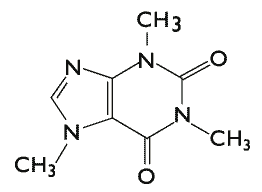
\includegraphics[width=\linewidth]{images/Caffeine_molecule.png}
\end{image}%
\tcblower
\end{figureptx}%
That is all rather informal, though, and to do mathematics we need very precise, formal definitions.  We now provide that.%
\end{subsectionptx}
%
%
\typeout{************************************************}
\typeout{Subsection 1.1.2 The formal definition of a graph}
\typeout{************************************************}
%
\begin{subsectionptx}{The formal definition of a graph}{}{The formal definition of a graph}{}{}{g:subsection:idp2}
The formal definition of a graph that we will use is the following:%
\begin{definition}{}{g:definition:idp3}%
A \emph{graph} \(G\) consists of a set \(V(G)\), called the \emph{vertices} of \(G\), and a set \(E(G)\), called the \emph{edges} of \(G\), of the two element subsets of \(V(G)\)%
\end{definition}
\begin{example}{}{g:example:idp4}%
Consider the water molecule, which consists of a single oxygen atom, connected to two hydrogen atoms.  It has three vertices, and so \(V(G)=\{O, H1, H2\}\), and two edges \(E(G)=\big\{\{O, H1\},\{O,H2\}\big\}\)%
\end{example}
This formal definition has some perhaps unintended consequences about what a graph is.  Because we have identified edges with the two things they connect, and have a set of edges, we can't have more than one edge between any two vertices.  In many real world examples, this is not the case: for example, on the London Tube, the Circle, District and Picadilly lines all connect Gloucester Road with South Kensington, and so there should be multiple edges between those two vertices on the graph.  As another example, in organic chemistry, there are often "double bonds", instead of just one.%
\par
Another consequence is that we require each edge to be a two element subset of \(V(G)\), and so we do not allow for the possibility of an edge between a vertex and itself, often called a \emph{loop}.%
\par
Graphs without multiple edges or loops are sometimes called \emph{simple graphs}.  We will sometimes deal with graphs with multiple edges or loops, and will try to be explicit when we allow this.  Our default assumption is that our graphs are simple.%
\par
Another consequence of the definition is that edges are symmetric, and work equally well in both directions.  This is not always the case: in road systems, there are often one-way streets.  If we were to model Twitter or Instragram as a graph, rather than the symmetric notion of friends we would have to work with ``following''.  To capture these, we have the notion of a \emph{directed graph}, where rather than just lines, we think of the edges as arrows, pointing from one vertex (the source) to another vertex (the target).  To model Twitter or Instagram, we would have an ege from vertex \(a\) to vertex \(b\) if \(a\) followed \(b\).%
\end{subsectionptx}
%
%
\typeout{************************************************}
\typeout{Subsection 1.1.3 Basic examples and concepts}
\typeout{************************************************}
%
\begin{subsectionptx}{Basic examples and concepts}{}{Basic examples and concepts}{}{}{g:subsection:idp5}
Several simple graphs that are frequently referenced have specific names.%
\begin{definition}{}{g:definition:idp6}%
The complete graph \(K_n\) is the graph on \(n\) vertices, with an edge between any two distinct vertices.%
\end{definition}
\begin{definition}{}{g:definition:idp7}%
The empty graph \(E_n\) is the graph on \(n\) vertices, with no edges.%
\end{definition}
\begin{definition}{}{g:definition:idp8}%
The path graph \(P_n\) is the graph on \(n\) vertices \(\{v_1,\dots, v_n\}\) with edges \(\{ \{v_1, v_2\}, \{v_2,v_3\},\dots,\{v_{n-1},v_n\}\}\).%
\end{definition}
\begin{definition}{}{g:definition:idp9}%
The cycle graph \(C_n\) is the graph on \(n\) vertices \(\{v_1,\dots, v_n\}\) with edges \(\{ \{v_1, v_2\}, \{v_2,v_3\},\dots,\{v_{n-1},v_n\}, \{v_n, v_1\}\}\).%
\end{definition}
\begin{figureptx}{Basic graphs}{x:figure:fig_basic_graphs}{}%
\begin{image}{0.05}{0.9}{0.05}%
\resizebox{\linewidth}{!}{%
\begin{tikzpicture}[scale=.5]
\node at (0,-3) {$K_5$};
\node at (6,-3) {$E_5$};
\node at (12, -3) {$P_5$};
\node at (18,-3) {$C_5$};


\begin{scope}[every node/.style={circle, draw, fill=red, inner sep=0pt, minimum width=4pt, thick}]
\draw \foreach \x in {90, 162,...,378}
{
    (\x:2) node {} -- (\x+72:2)
    (\x:2) -- (\x+144:2)
}; 


\begin{scope}[xshift=6cm]
\draw \foreach \x in {90, 162,...,378}
{
    node at (\x:2) {}
};    
\end{scope}
 
\begin{scope}[xshift=12cm]
\draw \foreach \x in {90, 162,...,306}
{
    (\x:2) node {} -- (\x+72:2)
}; 
\node at (378:2) {};
\end{scope}

\begin{scope}[xshift=18cm]
\draw \foreach \x in {90, 162,...,378}
{
    (\x:2) node {} -- (\x+72:2)
}; 
\end{scope}
\end{scope}
\end{tikzpicture}
}%
\end{image}%
\tcblower
\end{figureptx}%
\begin{definition}{}{g:definition:idp10}%
The complelement of a simple graph \(G\), which we will denote \(G^c\), and is sometimes written \(\overline{G}\), is the graph with the same vertex set as \(G\), but \(\{v,w\}\in E(G^c)\) if and only if \(\{v,w\}\notin E(G)\); that is, there is an edge between \(v\) and \(w\) in \(G^c\) if and only if there is not an edge between \(v\) and \(w\) in \(G\)%
\end{definition}
\begin{example}{}{g:example:idp11}%
The empty graph and complete graph are complements of each other; \(K_n^c=E_n\)%
\par
The path graph \(P_4\) and its complement are shown below:%
\begin{image}{0.05}{0.9}{0.05}%
\resizebox{\linewidth}{!}{%
\begin{tikzpicture}
\node at (.5,1.5) {$P_4$};
\node at (3.5,1.5) {$P_4^c$};


\begin{scope}[every node/.style={circle, draw, fill=red, inner sep=0pt, minimum width=4pt, thick}]
\node (a) at (0,0) {};
\node (b) at (0,1) {};
\node (c) at (1,1) {};
\node (d) at (1,0) {};
\draw (a)--(b)--(c)--(d);
\end{scope}

\begin{scope}[xshift=3cm, every node/.style={circle, draw, fill=red, inner sep=0pt, minimum width=4pt, thick}]
\node (a) at (0,0) {};
\node (b) at (0,1) {};
\node (c) at (1,1) {};
\node (d) at (1,0) {};
\draw (c)--(a)--(d)--(b);
\end{scope}
\end{tikzpicture}
}%
\end{image}%
\end{example}
It commonly occurs that there are two different types of vertices, and the edges only go between vertices of the two types.  For example, we may be modelling a company, and one type of vertices may represent the employees, and another type of vertices could represent the different jobs that need done, with an edge between a worker and a job if the worker is qualified to do that particular job.  We call these graphs \emph{bipartite}.%
\begin{definition}{}{g:definition:idp12}%
A graph \(\bfG\) is \emph{bipartite} if its vertices can be coloured red and blue so that every edge goes between a red vertex and a blue vertex.%
\end{definition}
\begin{example}{}{g:example:idp13}%
The graph below is bipartite.%
\begin{image}{0.05}{0.9}{0.05}%
\resizebox{\linewidth}{!}{%
\begin{tikzpicture}

\begin{scope}[every node/.style={circle, draw, fill=red, inner sep=0pt, minimum width=4pt, thick}]
\node (a) at (0,0) {};
\node (b) at (2,0) {};
\node (c) at (4,0) {};
\node (x) at (1,-2) {};
\node (y) at (3, -2) {};
\draw (a)--(x)--(b)--(y)--(c)--(x);
\end{scope}

\end{tikzpicture}
}%
\end{image}%
\end{example}
As another example, note that the cycle graph \(C_4\) is bipartite -{}-{} we can colour vertices 1 and 3 red, and vertices 2 and 4 blue.  But the cycle graph \(C_3\) is \emph{not} bipartite: as the two colours are interchangable, we can assume we coloured vertex 1 red; then since it is adjacent to both 2 and 3, those vertices must both be blue, but they're adjacent to each other, which violates the definition of bipartite.  More generally, we have:%
\begin{lemma}{}{}{g:lemma:idp14}%
The cycle graph \(C_n\) is bipartite if and only if n is even.%
\end{lemma}
\begin{proof}{}{g:proof:idp15}
Let's try to colour the vertices of \(C_n\) red and blue so that adjacent vertices have different colour.  Without loss of generality, we may assume that \(v_1\) is coloured blue.  Then since it is adjacent to \(v_1, v_2\) must be coloured red.  Continuing in this way, we see that \(v_k\) is blue for odd \(k\) and red for even \(k\).  But \(v_n\) is adjacent to \(v_1\), and so these will have different colours precisely when \(n\) is even.%
\end{proof}
\begin{lemma}{}{}{g:lemma:idp16}%
A graph \(\bfG\) is bipartite if and only if \(\bfG\) has no subgraphs that are isomorphic to \(C_{2k+1}\)%
\end{lemma}
\begin{proof}{}{g:proof:idp17}
First, note that if \(\bfG_2\) is a subgraph of \(\bfG_1\), and \(\bfG_1\) is bipartite, then so is \(\bfG_2\): colouring the vertices of \(\bfG_1\) red and blue in particular colours the vertices of \(\bfG_2\) as well.  Hence, we see if that \(\bfG\) has a subgraph isomorphic to \(C_{2k_1}\), which isn't bipartite by the previous lemma, then \(\bfG_1\) can't be bipartite, either.%
\par
In the other direction, we assume that \(\bfG\) has no subgraphs isomorphic to \(C_{2k+1}\); we need to prove that \(\bfG\) is bipartite.  Again, let's try to colour the vertices of \(\bfG\) red and blue so that adjancent vertices have different colours.  Choose a vertex \(v\) of \(\bfG\), without loss of generality we may assume that \(v\) is coloured blue; then all vertices adjacent to \(v\) -{}-{} i.e., those vertices at distance 1 from \(v\) -{}-{} are coloured red.  The vertices adjacent to those must be blue, and the ones adjacent to those must be red, alternating out.  This suggests trying to colour all vertices at odd distance from \(v\) red, and those vertices at even distance from \(v\) blue.  We will show that if this colouring has two vertices of the same colour that are adjacent, then \(\bfG\) has an odd cycle.%
\par
Assume that \(u\) and \(w\) are two vertices coloured red that are adjacent.  Since \(u\) is red, the distance from \(v\) to \(u\) is odd -{}-{} there is a path \(v=v_0 - v_1 - \cdots - v_{2k+1}=u\).  Similarly, there is an odd length path from \(v\) to \(w\): \(v=w_0 - w_1 - \cdots - w_{2\ell+1}=w\).  Taking the union of these two subgraphs and the edge connecting \(u\) and \(w\), we get a closed walk consisting of \((2k+1)+(2\ell+1)+1=2k+2\ell+3\) edges, which is odd.  This walk may repeat some vertices and edges, but if it does we can split it into two smaller walks, one of which must have odd length, and eventually we must get a closed walk of odd length that doesn't repeat any vertices.%
\par
The case that \(u\) and \(w\) are both coloured blue is completely analogous, except we will be merging two paths with an even number of edges and one extra edge to get a path with odd length.%
\end{proof}
A special type of bipartite graph is the complete bipartite graphs \(K_{m,n}\), which are the simple graphs that have as many edges as possible while still being bipartite.%
\begin{definition}{}{g:definition:idp18}%
The \emph{complete bipartite graph} \(K_{m,n}\) is the graph with \(m\) red vertices and \(n\) blue vertices, and an edge between very red vertex and every blue vertex.%
\end{definition}
\begin{example}{}{g:example:idp19}%
The complete bipartite graph \(K_{2,2}\) is isomorphic to \(C_4\).%
\par
The graphs \(K_{1,3}\) and \(K_{4,4}\) are drawn below.%
\begin{image}{0.05}{0.9}{0.05}%
\resizebox{\linewidth}{!}{%
\begin{tikzpicture}[scale=.5]
\node at (1,-1) {$K_{1,3}$};
\node at (5,-1) {$K_{4,4}$};

\begin{scope}[every node/.style={circle, draw, fill=red, inner sep=0pt, minimum width=4pt, thick}]

\foreach \x in {0,1,2}
{
    \draw (0,1)--(2,\x);
    \node at (2,\x) {};
};
\node at (0,1) {};

\begin{scope}[xshift=4cm]
\foreach \x in {0, 1,...,3}
{


    \foreach \y in {0,1,...,3}
    {
        \draw (0,\x) -- (2,\y);
	}
    \node at (0,\x) {};
    \node at (2,\x) {};
};
\end{scope}
\end{scope}
\end{tikzpicture}
}%
\end{image}%
\end{example}
\end{subsectionptx}
\end{sectionptx}
%
%
\typeout{************************************************}
\typeout{Section 1.2 Degree and handshaking}
\typeout{************************************************}
%
\begin{sectionptx}{Degree and handshaking}{}{Degree and handshaking}{}{}{x:section:s_intro_degrees}
%
%
\typeout{************************************************}
\typeout{Subsection 1.2.1 Definition of degree}
\typeout{************************************************}
%
\begin{subsectionptx}{Definition of degree}{}{Definition of degree}{}{}{g:subsection:idp20}
Intuitively, the \emph{degree} of a vertex is the ``number of edges coming out of it''. If we think of a graph \(G\) as a picture, then to find the degree of a vertex \(v\in V(G)\) we draw a very small circle around \(v\), the number of times the \(G\) intersects that circle is the degree of \(v\).  Formally, we have:%
\begin{definition}{}{g:definition:idp21}%
Let \(G\) be a simple graph, and let \(v\in V(G)\) be a vertex of \(G\).  Then the \emph{degree of \(v\)}, written \(d(v)\), is the number of edges \(e\in E(G)\) with \(v\in e\). Alternatively, \(d(v)\) is the number of vertices \(v\) is adjacent to.%
\end{definition}
\begin{example}{}{g:example:idp22}%
\begin{figureptx}{The graph \(K\)}{x:figure:fig_trumpet_graph}{}%
\begin{image}{0.25}{0.5}{0.25}%
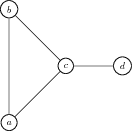
\includegraphics[width=\linewidth]{images/degreeexamplegraph.png}
\end{image}%
\tcblower
\end{figureptx}%
In the graph \(K\) shown in \hyperref[x:figure:fig_trumpet_graph]{Figure~{\xreffont\ref{x:figure:fig_trumpet_graph}}}, vertices \(a\) and \(b\) have degree 2, vertex \(c\) has degree 3, and vertex \(d\) has degree 1.%
\end{example}
Note that in the definition we require \(G\) to be a simple graph.  The notion of degree has a few pitfalls to be careful of \(G\) has loops or multiple edges.  We still want to the degree \(d(v)\) to match the intuitive notion of the ``number of edges coming out of \(v\)'' captured in the drawing with a small circle.  The trap to beware is that this notion no longer agrees with ``the number of vertices adjacent to \(v\)'' or the ``the number of edges incident to \(v\)''%
\begin{example}{}{g:example:idp23}%
\begin{sidebyside}{2}{0.025}{0.025}{0.05}%
\begin{sbspanel}{0.5}[center]%
The graph \(G\) to the right has two vertices, \(a\) and \(b\), and three edges, two between \(a\) and \(b\), and a loop at \(a\).  Vertex \(a\) has degree 4, and vertex \(b\) has degree 2.%
\end{sbspanel}%
\begin{sbspanel}{0.4}[center]%
\resizebox{\linewidth}{!}{%
\begin{tikzpicture}[scale=2, every loop/.style={}, bend angle=10]

\node[draw=black, circle] (a) at (1,0) {$a$};
\node[draw=black, circle] (b) at (0,0) {$b$};

\draw (a) edge[bend left] (b);
\draw (a) edge[bend right] (b);
\draw (a) edge[loop right] (a);

\end{tikzpicture}
}%
\end{sbspanel}%
\end{sidebyside}%
\end{example}
\end{subsectionptx}
%
%
\typeout{************************************************}
\typeout{Subsection 1.2.2 Extended example: Chemistry}
\typeout{************************************************}
%
\begin{subsectionptx}{Extended example: Chemistry}{}{Extended example: Chemistry}{}{}{g:subsection:idp24}
In organic chemistry, molecules are frequently drawn as graphs, with the vertices being atoms, and an edge betwen two vertices if and only if the corresponding atoms have a covalent bond between them (that is, they share a vertex).%
\begin{example}{Alkanes.}{g:example:idp25}%
\end{example}
The location of an element on the periodic table determines the valency of the element -{}-{} hence the degree that vertex has in any molecule containing that graph:%
%
\begin{itemize}[label=\textbullet]
\item{}Hydrogen (H) and Fluorine (F) have degree 1%
\item{}Oxygen (O) and Sulfur (S) have degree 2%
\item{}Nitrogen (N) and Phosphorous (P) have degree 3%
\item{}Carbon (C) has degree 4%
\end{itemize}
Usually, most of the atoms involved are carbon and hydrogen. Carbon atoms are not labelled with a C, but just left blank, while hydrogen atoms are left off completely. One can then complete the full structure of the molecule using the valency of each vertex.  On the exam, you may have to know that Carbon has degree 4 and Hydrogen has degree 1; the valency of any other atom would be provided to you%
\par
Graphs coming from organic chemistry do not have to be simple – sometimes there are double bonds, where a pair of carbon atoms have two edges between them.%
\begin{example}{}{g:example:idp26}%
Saturated vs. unsaturated\end{example}
If we know the chemical formula of a molecule, then we know how many vertices of each degree it has.  For a general graph, this information is known as the degree sequence%
\begin{definition}{Degree sequence.}{g:definition:idp27}%
The degree sequence of a graph is just the list (with multiplicity) of the degrees of all the vertices.%
\end{definition}
The following sage code draws a random graph with 7 vertices and 10 edges, and then gives its degree sequence.  You can tweak the code to generate graphs with different number of vertices and edges, and run the code multiple times, and the degree sequence should become clear.%
\begin{sageinput}
vertices = 7
edges = 10
g = graphs.RandomGNM(vertices,edges)
g.show()
print g.degree_sequence()
\end{sageinput}
Knowing the chemical composition of a molecule determines the degree sequence of its corresponding graph. However, it is possible that the same set of atoms may be put together into a molecule in more than one different ways. In chemistry, these are called \emph{isomers}.  In terms of graphs, this corresponds to different graphs that have the same degree sequence.%
\par
An important special case is the constant degree sequence.%
\begin{definition}{Regular graphs.}{g:definition:idp28}%
A graph \(\Gamma\) is \(d\)-\emph{regular}, or \emph{regular of degree} \(d\) if every vertex \(v\in\Gamma\) has the same degree \(d\), i.e. \(d(v)=d\).%
\end{definition}
As a common special case, a regular graph where every vertex has degree three is called \emph{trivalent}, or \emph{cubic}.%
\par
Some quick examples:%
\begin{enumerate}
\item{}The cycle graph \(C_n\) is two-regular%
\item{}The complete graph \(K_n\) is \((n-1)\)-regular%
\item{}The Petersen graph is trivalent%
\end{enumerate}
%
\end{subsectionptx}
%
%
\typeout{************************************************}
\typeout{Subsection 1.2.3 Handshaking lemma and first applications}
\typeout{************************************************}
%
\begin{subsectionptx}{Handshaking lemma and first applications}{}{Handshaking lemma and first applications}{}{}{g:subsection:idp29}
To motivative the Handshaking Lemma, we consider the following question.  Suppose there seven people at a party.  Is it possible that everyone at the party knows exactly three other people?%
\par
We can model the situation a graph, with vertices being people at the party, and an edge between two vertices if the corresponding people know each other.  The question is then asking for the existence of a graph with seven vertices so that every vertex has degree three.  It is then natural to attempt to solve the problem by trying to draw such a graph.  After a few foiled attempts, we begin to suspect that it's not possible, but doing a case-by-case elimination of all the possibilities is daunting.  It's easier to find a reason why we can't draw such a graph.%
\par
We will do this as follows: suppose that everyone at the party who knows each other shakes hands.  How many handshakes will occur?  On the one hand, from the definitions this would just be the number of edges in the graph.  On the other hand, we can count the number of handshakes working person-by-person: each person knows three other people, and so is involved in three handshakes.  But each handshake involves two people, and so if we count \(7*3\) we've counted each handhsake twice, and so there should be \(7*3/2=10.5\) handshakes happening, which makes no sense, as we can't have half a handshake.  Thus, we have a contradiction, and we conclude such a party isn't possible.%
\par
Euler's handshaking Lemma is a generalization of the argument we just made to an arbitrary graph.%
\begin{theorem}{}{}{g:theorem:idp30}%
(Euler's handshaking Lemma)%
%
\begin{equation*}
\sum_{v\in V(G)}d(v)=2|E(G)|
\end{equation*}
\end{theorem}
\begin{proof}{}{g:proof:idp31}
We count the ``ends'' of edges two different ways.  On the one hand, every end occurs at a vertex, and at vertex \(v\) there are \(d(v)\) ends, and so the total number of ends is the sum on the left hand side. On the other hand, every edge has exactly two ends, and so the number of ends is twice the number of edges, giving the right hand side.%
\end{proof}
We have seen already seen one use of Euler's handshaking Lemma, but it will be particularly useful in Chapter 3, when we study graphs on surfaces.%
\end{subsectionptx}
\end{sectionptx}
%
%
\typeout{************************************************}
\typeout{Section 1.3 Graph Isomorphisms}
\typeout{************************************************}
%
\begin{sectionptx}{Graph Isomorphisms}{}{Graph Isomorphisms}{}{}{x:section:s_intro_isomorphisms}
\begin{introduction}{}%
Generally speaking in mathematics, we say that two objects are "isomorphic" if they are "the same" in terms of whatever structure we happen to be studying.  The symmetric group \(S_3\) and the symmetry group of an equilateral triangle \(D_6\) are isomorphic.  In this section we briefly briefly discuss isomorphisms of graphs.%
\end{introduction}%
%
%
\typeout{************************************************}
\typeout{Subsection 1.3.1 Isomorphic graphs}
\typeout{************************************************}
%
\begin{subsectionptx}{Isomorphic graphs}{}{Isomorphic graphs}{}{}{g:subsection:idp32}
The "same" graph can be drawn in the plane in multiple different ways.  For instance, the two graphs below are each the "cube graph", with vertices the 8 corners of a cube, and an edge between two vertices if they're connected by an edge of the cube:%
\begin{figureptx}{Two drawings of the cube graph}{g:figure:idp33}{}%
\begin{image}{0.05}{0.9}{0.05}%
\resizebox{\linewidth}{!}{%
\tikzstyle{every node}=[circle, draw, fill=red, inner sep=0pt, minimum width=4pt]

\begin{tikzpicture}[thick]
  \node (a) at (0,0) {};
  \node (b) at (0,3) {};
  \node (c) at (3,3) {};
  \node (d) at (3,0) {};
  \node (e) at (1,1) {};
  \node (f) at (1,2) {};
  \node (g) at (2,2) {};
  \node (h) at (2,1) {};

  \draw (a)--(b)--(c)--(d)--(a)--(e)--(f)--(g)--(h)--(e);
  \draw (b)--(f);
  \draw (c)--(g);
  \draw (d)--(h);

  \begin{scope}[xshift=4cm, yshift=1.5cm, scale=1.5]
  \node (a) at (0,0) {};
  \node (b) at (1,1) {};
  \node (c) at (2,0) {};
  \node (d) at (1,-1) {};
  \node (e) at (1,0) {};
  \node (f) at (2,1) {};
  \node (g) at (3,0) {};
  \node (h) at (2,-1) {};

  \draw (a)--(b)--(c)--(d)--(a)--(e)--(f)--(g)--(h)--(e);
  \draw (b)--(f);
  \draw (c)--(g);
  \draw (d)--(h);



    \end{scope}

\end{tikzpicture}
}%
\end{image}%
\tcblower
\end{figureptx}%
\begin{example}{}{g:example:idp34}%
It is not hard to see that the two graphs above are both drawings of the cube, but for more complicated graphs it can be quite difficult at first glance to tell whether or not two graphs are the same.  For instance, there are many ways to draw the Petersen graph that aren't immediately obvious to be the same.%
\par
This \href{https://msollami.com/code/2014/12/24/graph-isomorphisms}{animated gif} created by Michael Sollami for \href{https://www.quantamagazine.org/algorithm-solves-graph-isomorphism-in-record-time-20151214/}{this Quanta Magazine article} on the Graph Isomorphism problem illustrates many different such drawings in a way that makes the isomorphisms apparent.%
\end{example}
\begin{definition}{}{g:definition:idp35}%
An isomorphism \(\varphi:G\to H\) of simple graphs is a biject \(\varphi:V(G)\to V(H)\) between their vertex sets that preserves the number of edges between vertices.  In other words, \(\varphi(v)\) and \(\varphi(w)\) are adjacent in \(H\) if and only if \(v\) and \(w\) are adjancent in \(G\).%
\end{definition}
\begin{example}{}{g:example:idp36}%
\begin{figureptx}{\(C_5\) is isomorphic to its complement \(C_5^c\)}{g:figure:idp37}{}%
\begin{image}{0.05}{0.9}{0.05}%
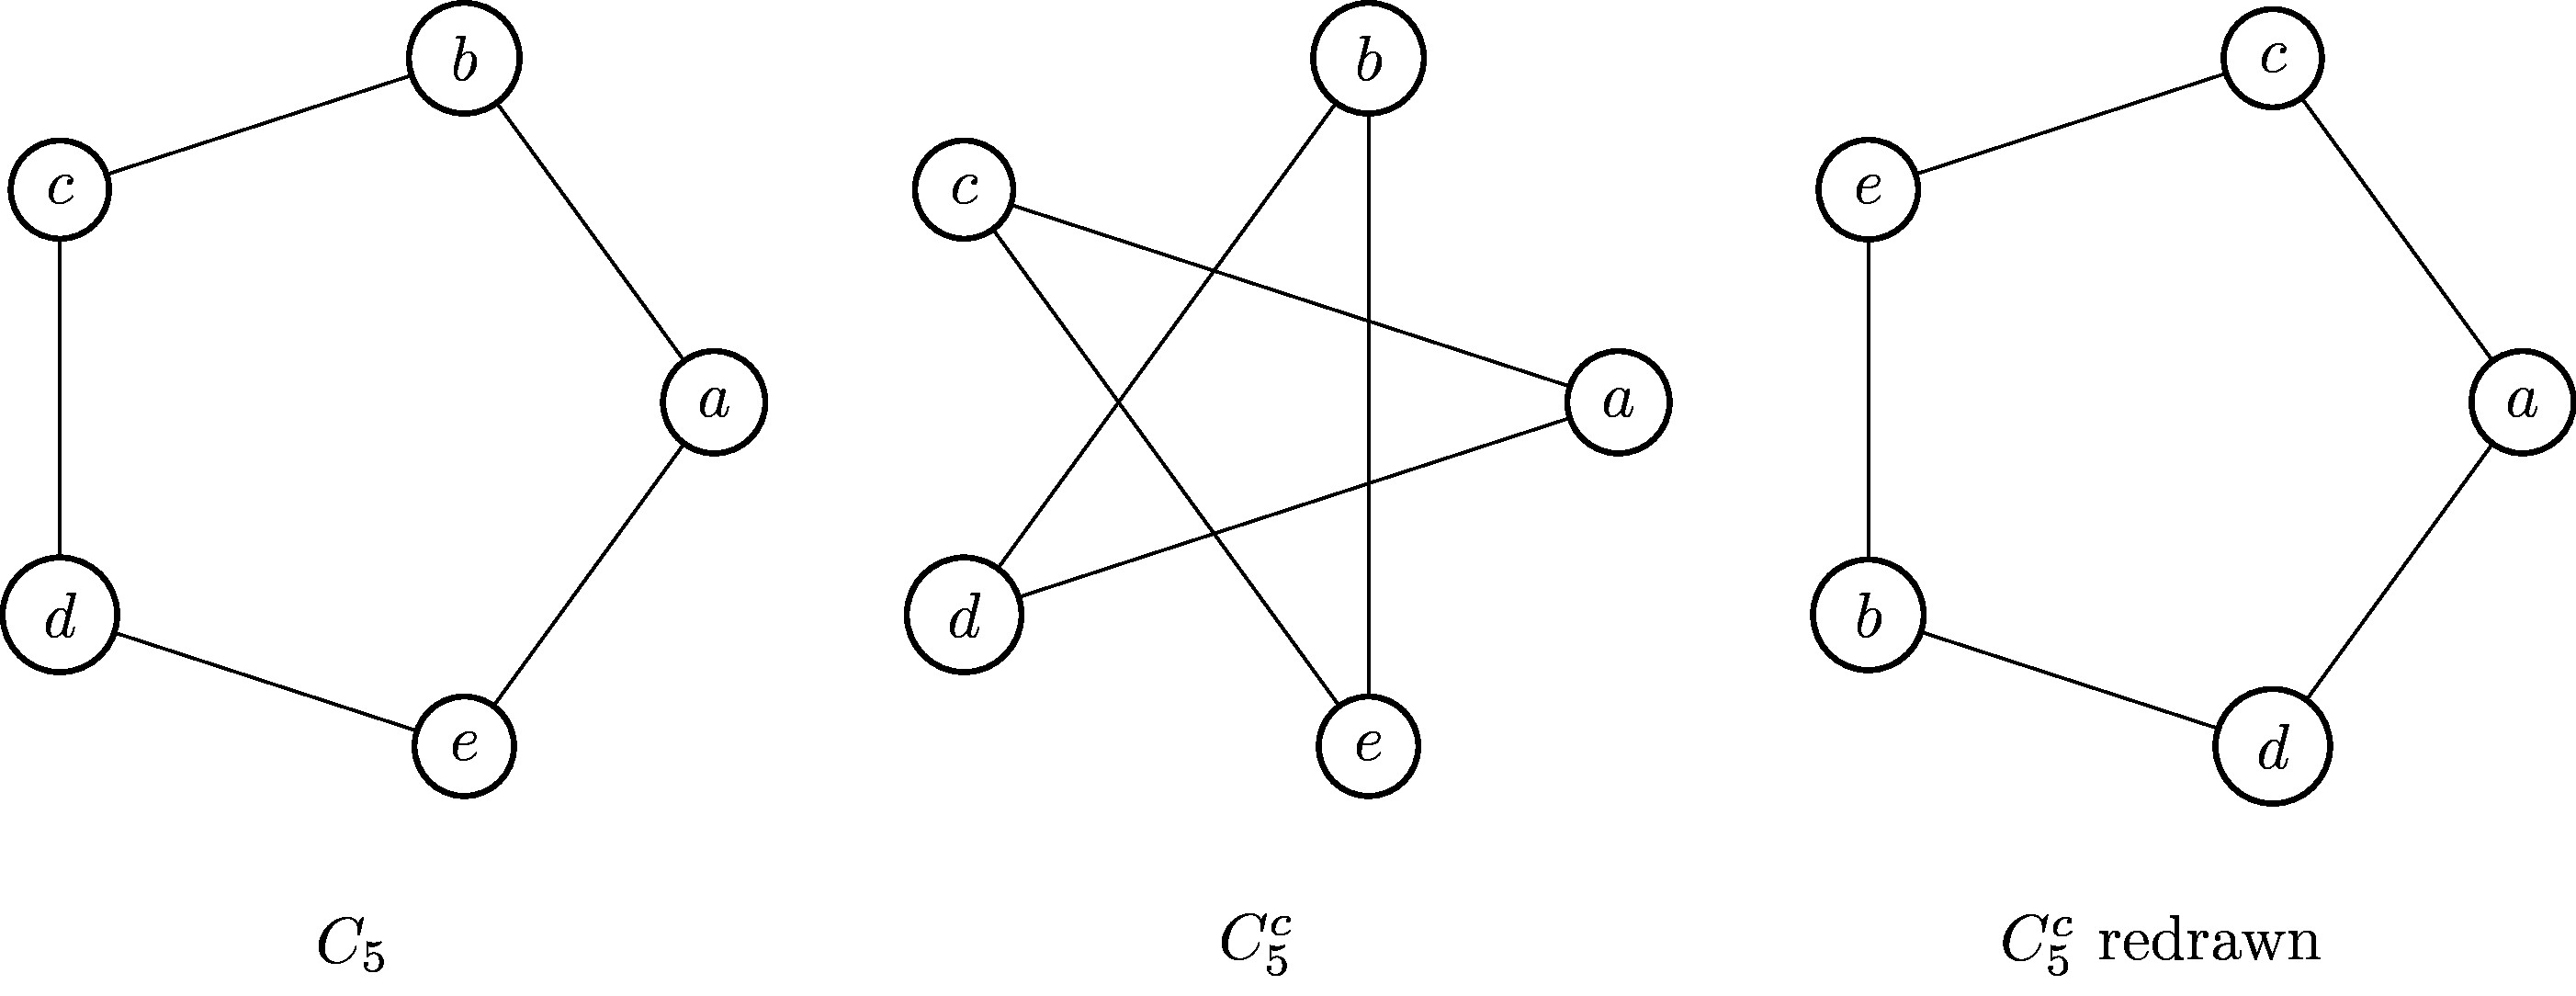
\includegraphics[width=\linewidth]{images/cycleandstar.jpg}
\end{image}%
\tcblower
\end{figureptx}%
The cycle graph on 5 vertices, \(C_5\) is isomorphic to its complement, \(C_5^c\).  The cycle \(C_5\) is usually drawn as a pentagon, and if we were then going to naively draw \(C_5^c\) we would draw a 5-sided star.  However, we could draw \(C_5^c\) differently as shown, making it clear that it is isomorphic to \(C_5\), with isomorphism \(\varphi:C_5\to C_5^c\) defined by \(\varphi(a)=a, \varphi(b)=c, \varphi(c)=e, \varphi(d)=b, \varphi(e)=d\).%
\end{example}
Although solving the graph isomorphism problem for general graphs is quite difficult, doing it for small graphs by hand is not too bad and is something you must be able to do for the exam.  If the two graphs are actually isomorphic, then you should show this by exhibiting an isomrophism; that is, writing down an explicit bijection between their vertex sets with the desired properties. The most attractive way of doing this, for humans, is to label the vertices of both copies with the same letter set.%
\par
If two graphs are not isomorphic, then you have to be able to prove that they aren't. Of course, one can do this by exhaustively describing the possibilities, but usually it's easier to do this by giving an obstruction – something that is different between the two graphs. One easy example is that isomorphic graphs have to have the same number of edges and vertices. We'll discuss some others in the next section%
\end{subsectionptx}
%
%
\typeout{************************************************}
\typeout{Subsection 1.3.2 Heuristics for showing graphs are or aren't isomorphic}
\typeout{************************************************}
%
\begin{subsectionptx}{Heuristics for showing graphs are or aren't isomorphic}{}{Heuristics for showing graphs are or aren't isomorphic}{}{}{g:subsection:idp38}
Another, only slightly more advanced invariant is the degree sequence of a graph that we saw last lecture in our discussion of chemistry.%
\par
If \(\varphi:G\to H\) is an isomorphism of graphs, than we must have \(d(\varphi(v))=d(v)\) for all vertices \(v\in G\), and since isomorphisms are bijections on the vertex set, we see the degree sequence must be preserved.  However, just because two graphs have the same degree sequences does not mean they are isomorphic.%
\par
Slightly subtler invariants are number and length of cycles and paths.%
\end{subsectionptx}
%
%
\typeout{************************************************}
\typeout{Subsection 1.3.3 Cultural Literacy: The Graph Isomorphism Problem}
\typeout{************************************************}
%
\begin{subsectionptx}{Cultural Literacy: The Graph Isomorphism Problem}{}{Cultural Literacy: The Graph Isomorphism Problem}{}{}{g:subsection:idp39}
This section, as all "Cultural Literacy" sections, is information that you may find interesting, but won't be examined.%
\par
The graph isomorphism problem is the following: given two graphs \(G\) and \(H\), determine whether or not \(G\) and \(H\) are isomorphic. Clearly, for any two graphs \(G\) and \(H\), the problem is solvable: if \(G\) and \(H\) both of \(n\) vertices, then there are \(n!\) different bijections between their vertex sets.  One could simply examine each vertex bijection in turn, checking whether or not it maps edges to edges.%
\par
The problem is interesting because the naive algorithm discussed above is not very efficient: for large \(n\), \(n!\) is absolutely huge, and so in general this algorithm will take a long time.  The question is, is there are a faster way to do check? How fast can we get?%
\par
The isomorphism problem is of fundamental importance to theoretical computer science. Apart from its practical applications, the exact difficulty of the problem is unknown. Clearly, if the graphs are isomorphic, this fact can be easily demonstrated and checked, which means the Graph Isomorphism is in NP.%
\par
Most problems in NP are known either to be easy (solvable in polynomial time, P), or at least as difficult as any other problem in NP (NP complete). This is not true of the Graph Isomorphism problem. In November of last year, Laszlo Babai announced a quasipolynomial-time algorithm for the graph isomorphism problem – you can read about this work in this great popular science article.%
\end{subsectionptx}
\end{sectionptx}
%
%
\typeout{************************************************}
\typeout{Section 1.4 Instant Insanity}
\typeout{************************************************}
%
\begin{sectionptx}{Instant Insanity}{}{Instant Insanity}{}{}{x:section:s_intro_instantinsanity}
\begin{introduction}{}%
So far, our motivation for studying graph theory has largely been one of philosophy and language.  Before we get too much deeper, however, it may be useful to present a nontrivial and perhaps unexpected application of graph theory; an example where graph theory helps us to do something that would be difficult or impossible to do without it.%
\end{introduction}%
%
%
\typeout{************************************************}
\typeout{Subsection 1.4.1 A puzzle}
\typeout{************************************************}
%
\begin{subsectionptx}{A puzzle}{}{A puzzle}{}{}{g:subsection:idp40}
\begin{figureptx}{Instant Insanity Package}{g:figure:idp41}{}%
\begin{image}{0.1}{0.8}{0.1}%

\includegraphics[width=\linewidth]{images/InstantInsanityPackage.JPG}
\end{image}%
\tcblower
\end{figureptx}%
There is a puazzle marketed under the name "Instant Insanity", one version of which is shown above.  The puzzle is sometimes called "the four cubes problem", as it consists of four different cubes.   Each face of each cube is painted one of four different colours: blue, green, red or yellow. The goal of the puzzle is to line the four cubes up in a row, so that along the four long edges (front, top, back, bottom) each of the four colours appears eactly once.%
\par
Depending on how the cubes are coloured, this may be not be possible, or there may be many such possibilities. In the original instant insanity, there is exactly one solution (up to certain equivalences of cube positions).  The point of the cubes is that there are a large number of possible cube configurations, and so if you just look for a solution without being extremely systematic, it is highly unlikely you will find it.%
\par
But trying to be systematic and logical about the search directly is quite difficult, perhaps because we have problems holding the picture of the cube in our mind.  In what follows, we will introduce a way to translate the instant insanity puzzle into a question in graph theory.  This is obviously in no way necessary to solve the puzzle, but does make it much easier.  It also demonstrates the real power of graph theory as a visualization and thought aid.%
\par
There are many variations on Instant Insanity, discussions of which can be found \href{http://www.cs.brandeis.edu/\~storer/JimPuzzles/ZPAGES/zzzInstantInsanity.html}{here} and \href{http://www.jaapsch.net/puzzles/insanity.htm}{here}. There’s also a \href{https://www.youtube.com/watch?v=CQ2gHSKZBEw}{commercial} for the game.%
\end{subsectionptx}
%
%
\typeout{************************************************}
\typeout{Subsection 1.4.2 Enter graph theory}
\typeout{************************************************}
%
\begin{subsectionptx}{Enter graph theory}{}{Enter graph theory}{}{}{g:subsection:idp42}
It turns out that the important factor of the cubes is what color is on the opposite side of each face.  Suppose we want face one facing forward.  Then we have four different ways to rotate the cube to keep this the same.  The same face will always appear on the opposite side, but we can get any of the remaining four faces to be on top, say.%
\begin{figureptx}{An impossible set of cubes}{x:figure:fig_impossible_cubes}{}%
\begin{image}{0}{1}{0}%
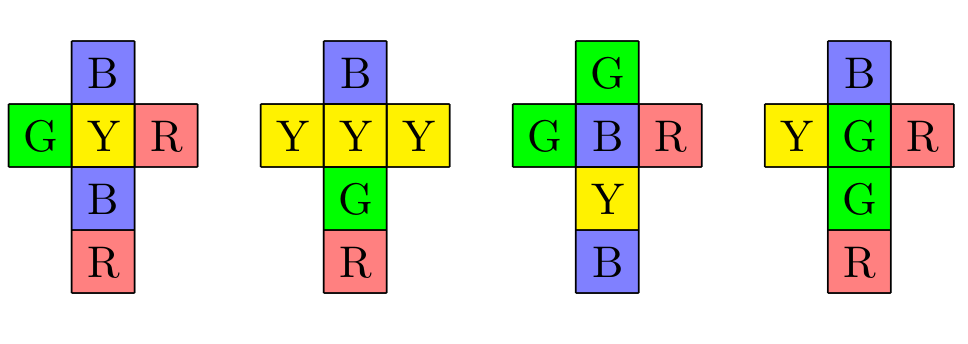
\includegraphics[width=\linewidth]{images/ImpossibleCubes.png}
\end{image}%
\tcblower
\end{figureptx}%
Let us encode this information in a graph.   The vertices of the graph will be the four colors, B, G, R and Y. We will put an edge between two colors each time they appear as opposite faces on a cube, and we will label that edge with a number 1-4 denoting which cube the two opposite faces appear. Thus, in the end the graph will have twelve edges, three with each label 1-4. For from the first cube, there will be a loop at B, and edge between G and R, and an edge between Y and R.  The graph corresponding to the four cubes above is the following:%
\begin{figureptx}{The graph constructed from the cubes in \hyperref[x:figure:fig_impossible_cubes]{Figure~{\xreffont\ref{x:figure:fig_impossible_cubes}}}}{x:figure:fig_graph_from_cubes}{}%
\begin{image}{0.05}{0.9}{0.05}%
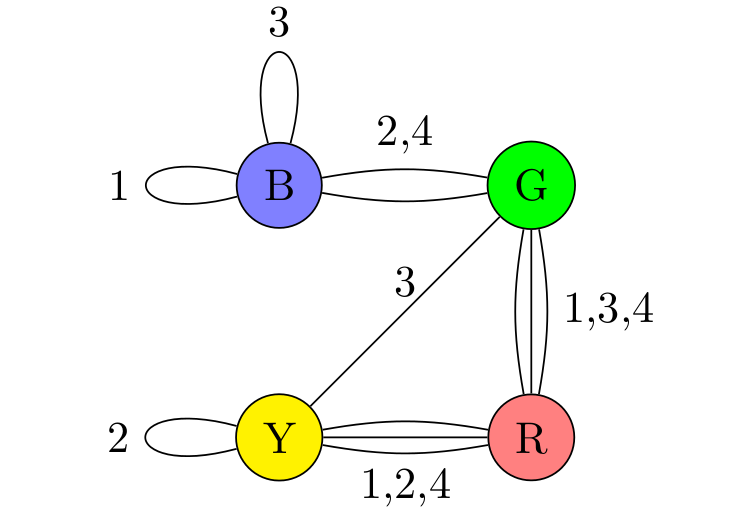
\includegraphics[width=\linewidth]{images/InstantInsanityImpossibleGraph.png}
\end{image}%
\tcblower
\end{figureptx}%
\end{subsectionptx}
%
%
\typeout{************************************************}
\typeout{Subsection 1.4.3 Proving that our cubes were impossible}
\typeout{************************************************}
%
\begin{subsectionptx}{Proving that our cubes were impossible}{}{Proving that our cubes were impossible}{}{}{g:subsection:idp43}
We now analyze the graph to prove that this set of cubes is not possible.%
\par
Suppose we had an arrangement of the cubes that was a solution. Then, from each cube, pick the edge representing the colors facing front and back on that cube. These four edges are a subgraph of our original graph, with one edge of each label, since we picked one edge from each cube. Furthermore, since we assumed the arrangement of cubes was a solution of instant insanity, each color appears once on the front face and once on the back. In terms of our subgraph, this translates into asking that each vertex has degree two.%
\par
We can get another subgraph satisfying these two properties by looking at the faces on the top and bottom for each cube and taking the corresponding edges. Furthermore, these two subgraphs do not have any edges in common.%
\par
Thus, given a solution to the instant insanity problem, we found a pair of subgraphs \(S_1, S_2\) satisfying:%
\begin{enumerate}
\item{}Each subgraph \(S_i\) has one edge with each label 1,2,3,4%
\item{}Every vertex of \(S_i\) has degree 2%
\item{}No edge of the original graph is used in both \(S_1\) and \(S_2\)%
\end{enumerate}
As an exercise, one can check that given a pair of subgraphs satisfying 1-3, one can produce a solution to the instant insanity puzzle.%
\par
Thus, to show the set of cubes we are currently examining does not have a solution, we need to show that the graph does not have two subgraphs satisfying properties 1-3.%
\par
To do, this, we catalog all graphs satisfying properties 1-2. If every vertex has degree 2, either:%
\begin{enumerate}
\item{}Every vertex has a loop%
\item{}There is one vertex with a loop, and the rest are in a triangle%
\item{}There are two vertices with loops and a double edge between the other two vertices%
\item{}There are two pairs of double edges%
\item{}All the vertices live in one four cycle%
\item{}A subgraphs of type 1 is not possible, because G and R do not have loops.%
\end{enumerate}
%
\par
For subgraphs of type 2, the only triangle is G-R-Y, and B does have loops. The edge between Y-G must be labeled 3, which means the loop at B must be labeled 1. This means the edge between G and R must be labeled 4 and the edge between Y and R must be 2, giving the following subgraph:%
\begin{figureptx}{A subgraph for a solution for one pair of faces}{x:figure:fig_impossible_first}{}%
\begin{image}{0.3}{0.4}{0.3}%
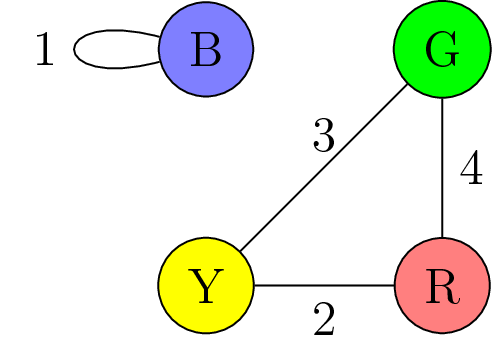
\includegraphics[width=\linewidth]{images/InstantInsanityImpossibleFirst.png}
\end{image}%
\tcblower
\end{figureptx}%
For type 3, the only option is to have loops at B and Y and a double edge between G and R. We see the loop at Y must be labeled 2, one of the edges between G and R must be 4, and the loop at B and the other edge between G and R can switch between 1 and 3, giving two possibilities:%
\begin{figureptx}{Two more subgraphs for a partial solutions}{x:figure:fig_impossible_twoandthree}{}%
\begin{sidebyside}{2}{0.05}{0.05}{0.1}%
\begin{sbspanel}{0.4}[center]%
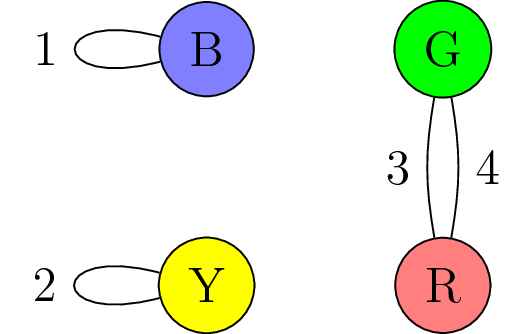
\includegraphics[width=\linewidth]{images/InstantInsanityImpossibleSecond.png}
\end{sbspanel}%
\begin{sbspanel}{0.4}[center]%
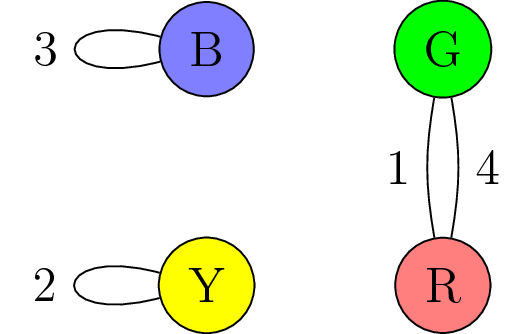
\includegraphics[width=\linewidth]{images/InstantInsanityImpossibleThird.png}
\end{sbspanel}%
\end{sidebyside}%
\tcblower
\end{figureptx}%
For subgraphs of type 4, the only option would be to have a double edge between B and G and another between Y and R; however, none of these edges are labeled 3 and this option is not possible.%
\par
Finally, subgraphs of type 5 cannot happen because B is only adjacent to G and to itself; to be in a four cycle it would have two be adjacent to two vertices that aren’t itself.%
\par
This gives three different possibilities for the subgraphs SiSi that satisfy properties 1 and 2. However, all three possibilities contain the the edge labeled 4 between G and R; hence we cannot choice two of them with disjoint edges, and the instant insanity puzzle with these cubes does not have a solution.%
\end{subsectionptx}
%
%
\typeout{************************************************}
\typeout{Subsection 1.4.4 Other cube sets}
\typeout{************************************************}
%
\begin{subsectionptx}{Other cube sets}{}{Other cube sets}{}{}{g:subsection:idp44}
The methods above also give a way to find the solution to a set of instant insanity cubes should one exist.  I illustrate this in the following Youtube video:%
\setlength{\qrsize}{9em}
\setlength{\previewwidth}{\linewidth}
\addtolength{\previewwidth}{-\qrsize}
\begin{tcbraster}[raster columns=2, raster column skip=1pt, raster halign=center, raster force size=false, raster left skip=0pt, raster right skip=0pt]%
\begin{tcolorbox}[previewstyle, width=\previewwidth]%
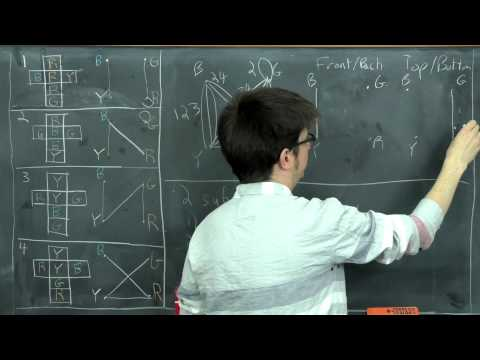
\includegraphics[width=0.80\linewidth,height=\qrsize,keepaspectratio]{images/video-1.jpg}%
\end{tcolorbox}%
\begin{tcolorbox}[qrstyle]%
{\hypersetup{urlcolor=black}\qrcode[height=\qrsize]{https://www.youtube.com/watch?v=GsbhRfjaaN8}}%
\end{tcolorbox}%
\begin{tcolorbox}[captionstyle]%
\small YouTube: \mono{https://www.youtube.com/watch?v=GsbhRfjaaN8}\end{tcolorbox}%
\end{tcbraster}%
\end{subsectionptx}
\end{sectionptx}
%
%
\typeout{************************************************}
\typeout{Section 1.5 Trees}
\typeout{************************************************}
%
\begin{sectionptx}{Trees}{}{Trees}{}{}{x:section:s_intro_trees}
\begin{introduction}{}%
A very important class of graphs are trees -{}-{} they are connected, but just barely: removing any edge causes them not to be connected.%
\end{introduction}%
%
%
\typeout{************************************************}
\typeout{Subsection 1.5.1 Basics on trees}
\typeout{************************************************}
%
\begin{subsectionptx}{Basics on trees}{}{Basics on trees}{}{}{g:subsection:idp45}
\begin{figureptx}{A forest consisting of three trees}{g:figure:idp46}{}%
\begin{image}{0.1}{0.8}{0.1}%
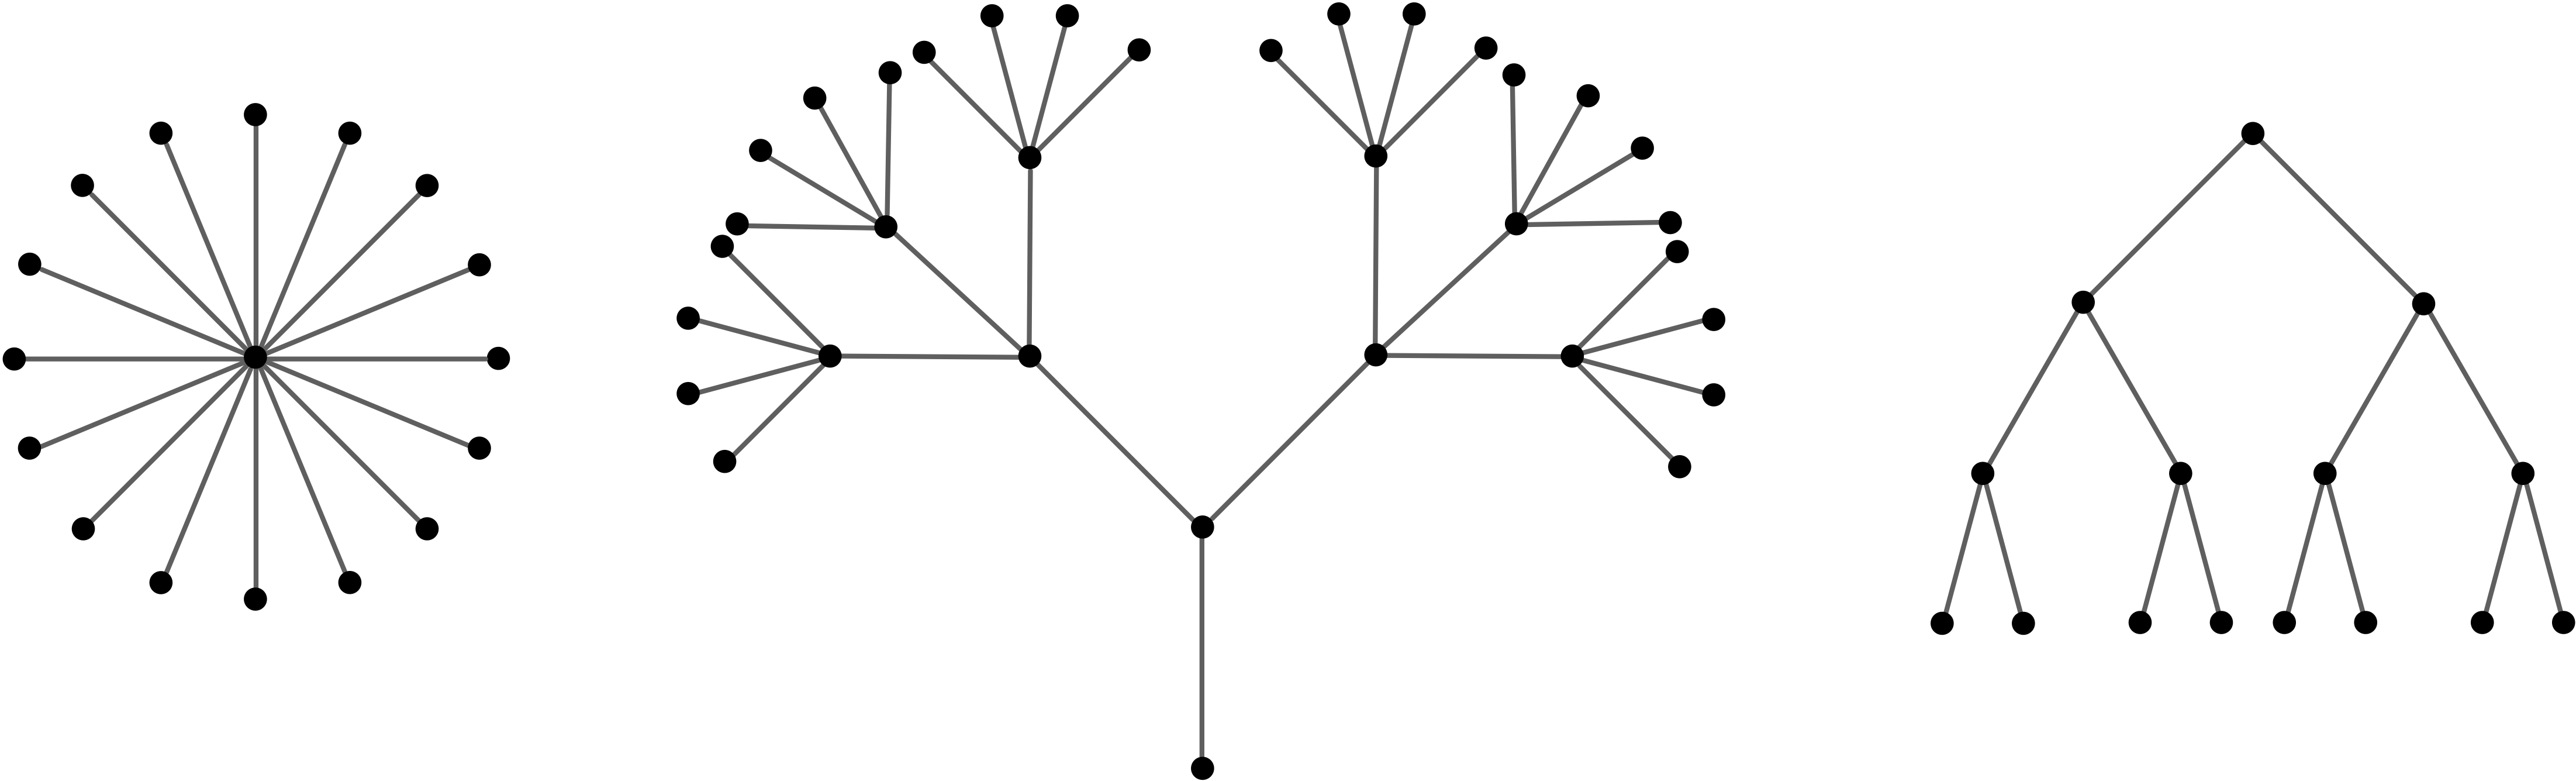
\includegraphics[width=\linewidth]{images/forest.png}
\end{image}%
\tcblower
\end{figureptx}%
The figure above shows some examples of the trees.  Meanwhile, the cycle graph \(\bfC_n\) or the complete graph \(\bfK_n\) with \(n\geq 3\) are not trees: we can remove an edge from these graphs and they'd still be connected. The formal definition of a tree is as follows:%
\begin{definition}{Trees and Forests.}{g:definition:idp47}%
A graph \(\bfG\) is a \emph{tree} if:%
%
\begin{enumerate}
\item{}\(\bfG\) is connected%
\item{}\(\bfG\) has no cycles%
\end{enumerate}
A not necessarily connected graph with no cycles is called a \emph{forest}, so that a forest is a union of trees.%
\end{definition}
Informally, the condition that \(\bfG\) is connected is asking that \(\bfG\) have enough edges, while the condition that \(\bfG\) has no cycles is asking for \(\bfG\) not to have too many edges.  Thus, trees are sort of "goldilocks" graphs -{}-{} they have enough edges, but not too many -{}-{} they're connected, but just barely.%
\par
The following Theorem gives many alternate characterisations of trees, and makes more precise the intuition of trees as "goldilocks graphs"%
. \begin{theorem}{}{}{g:theorem:idp48}%
Let \(\bfG\) be a graph with \(n\) vertices.  The following are equivalent:%
%
\begin{enumerate}
\item{}\(\bfG\) is a tree.%
\item{}Between any two vertices \(a,b\in V(\bfG)\), there is a unique path.%
\item{}\(\bfG\) is connected, but removing any edge makes \(\bfG\) disconnected.%
\item{}\(\bfG\) has no cycles, but adding any edges to \(\bfG\) creates a cycle.%
\item{}\(\bfG\) is connected and has \(n-1\) edges%
\item{}\(\bfG\) has no cycles and has \(n-1\) edges%
\end{enumerate}
\end{theorem}
We will not use most of , and will not prove that all options are equivalence.  We briefly proof that 1 is equivalent to 2 now, and in the next section we will carefully prove that 1 is equivalent to 5, as we will use this fact a few times.  The rest make a good exercise to check your basic understanding.%
\par
To see that 1 and 2 are equivalent, note that being connected by definition means there is a path between every two vertices.  As a tree is a connected graph without any cycles, to finish seeing 1 and 2 are equivalent is exactly \hyperref[x:lemma:lemma-unique-cycle]{Lemma~{\xreffont\ref{x:lemma:lemma-unique-cycle}}}, whose main idea is contained in \hyperref[x:figure:fig-unique-cycle]{Figure~{\xreffont\ref{x:figure:fig-unique-cycle}}}%
\begin{figureptx}{Two different paths create a cycle}{x:figure:fig-unique-cycle}{}%
\begin{image}{0.05}{0.9}{0.05}%
\resizebox{\linewidth}{!}{%
\begin{tikzpicture}[scale=.5]
\begin{scope}[every node/.style={circle, draw, fill=red, inner sep=0pt, minimum width=4pt, thick}]

\draw node (a) at (0,0) {$v$};
  \draw node (b) at (2.1,.9) {};
  \draw node (c) at (4,1.3) {};
  \draw node (d) at (6,0) {$w$};
  \draw node (e) at (5.1,-1) {};
  \draw node (f) at (3.4, -1.4) {};
  \draw node (g) at (.5, -.8) {};
  \draw[red, dashed] (a)--(b)--(c)--(d);
  \draw[blue, dotted] (d)--(e)--(f)--(g)--(a);
  \end{scope}

\begin{scope}[xshift=8cm, every node/.style={circle, draw, fill=red, inner sep=0pt, minimum width=4pt, thick}]
  \draw node (a) at (0,0) {$v$};
  \draw node (b) at (.5,.5) {};
  \draw node (c) at (2.5, 1) {};
  \draw node (d) at (4.4,.3) {};
    \draw node (e) at (5.5,.8) {};
    \draw node (f) at (6, 0) {$w$};
    
    \draw node (g) at (2, -.3) {};
    \draw node (h) at (2.4, -1) {};
    \draw node (i) at (1.7, -.8) {};
    \draw node (j) at (5.8, -.7) {};
    

    
  \draw[red, dashed] (a)--(b)--(c)--(d)--(e)--(f);
  \draw[blue, dotted] (a)--(b)--(g)--(h)--(i)--(g)--(d)--(j)--(f);
  \end{scope}

\end{tikzpicture}
}%
\end{image}%
\tcblower
\end{figureptx}%
\begin{lemma}{}{}{x:lemma:lemma-unique-cycle}%
A graph \(\bfG\) has no cycles if and only if there is at most one path between any two vertices of \(\bfG\).%
\end{lemma}
\begin{proof}{}{g:proof:idp49}
If \(\bfG\) has a cycle, the there are at least two paths between any vertex on that cycle -{}-{} the paths going each way around the cycle.  Thus, we just have to show that if there there are two paths between between \(v\) and \(w\), then \(\bfG\) has a cycle.%
\par
In the easy case, the two paths will contain no vertices in common except for \(v\) and \(w\), and so the union of the two paths will be a cycle.  In general, the paths will share other vertices and edges -{}-{} they may well repeat vertices and edges themselves.  But in any case, by considering some subset of these two paths will be a cycle.%
\end{proof}
\end{subsectionptx}
%
%
\typeout{************************************************}
\typeout{Subsection 1.5.2 Leaves}
\typeout{************************************************}
%
\begin{subsectionptx}{Leaves}{}{Leaves}{}{}{g:subsection:idp50}
To prove Theorem , we first need to introduce the concept of leaves.%
\begin{definition}{Leaf.}{g:definition:idp51}%
A vertex \(v\in\bfG\) is called a \emph{leaf} if it has degree one, i.e. if \(d(v)=1\)%
\end{definition}
When looked at a drawn graph, this definition is fairly intuitive: real life trees branch out and split in leaves, just like mathematical trees.%
\begin{lemma}{Trees have leaves.}{}{g:lemma:idp52}%
Let \(\bfT\) be a finite tree with at least two vertices.  Then \(\bfT\) has at least two leaves.\end{lemma}
\begin{proof}{}{g:proof:idp53}
By assumption, \(\bfT\) has at least two vertices, say \(v_0\) and \(w_0\).  Since \(\bfT\) is a tree it is connected, and so in particular there must be a path between \(v_0\) and \(w_0\); let \(v_i\) be the vertices in this path, and let \(e_i\) be the edge in the path joining \(v_{i-1}\) to \(v_i\).%
\par
Since \(v_m\) is adjacent to \(e_m\) it has degree at least one; if it has degree 1 it is a leaf, and we've found a leaf.  If \(v_m\) is not a leaf, then there must be another edge coming out of it, say \(e_{m+1}\) going to \(v_{m+1}\).  Note that \(v_{m+1}\) cannot be any of the vertices we've already found, as then we'd have more than one path between two vertices and hence a loop, but \(\bfT\) was a tree.  Thus we can make the path a bit longer.%
\par
We can now continue this argument inductively as long as the vertex at the of the path has degree higher than 1.  But since \(\bfT\) is finite, and we never return to a vertex we've already visited, we this process must eventually terminate, but the only way this can happen is if the end vertex of the path has degree 1, that is, if it's a leaf.%
\par
A similar argument extending from \(v_0\), the other end of the path, shows that we must eventually reach a different leaf from that end, and so \(\bfT\) must have at least two leaves, as desired.%
\end{proof}
 Now that we have a basic understanding of leaves, we are ready to prove the following: \begin{lemma}{}{}{g:lemma:idp54}%
A simple graph \(\bfG\) with \(n\) vertices is a tree if and only if is connected and has \(n-1\) edges.%
\end{lemma}
\begin{proof}{}{g:proof:idp55}
Since being connected is half of the requirement of being a tree, we need to show that a connected graph on \(n\) vertices is a tree if and only if it has \(n-1\) edges.%
\par
Let us first prove that a tree on \(n\) vertices has \(n-1\) edges.  We will use induction on \(n\).  As bases, there is only one tree with 1 vertex, and it does in fact have 0 edges, and there is only one tree with two vertices, and it does in fact have 1 edge.  So for the inductive step, let us suppose that we know that all trees with \(k\lt n\) vertices have \(k-1\) edges, and let \(\bfT\) be a tree with \(n\) vertices.  By Lemma, we know that \(\bfT\) has a leaf \(v\), which by the definition of leaves is connected to the rest of \(\bfT\) by a single edge \(e\).  If we delete \(v\) and \(e\) from \(\bfT\), we get a smaller graph \(\bfT^\prime\) ince which has one less vertex and one less edge than \(\bfT\) did.%
\par
Since \(\bfT\) was a tree, it follows that \(\bfT^\prime\) is a tree, too -{}-{} check this yourself, using the definition of a tree!  Then, since \(\bfT^\prime\) is a tree with \(n-1\) vertices, byt the inductive hypothesis it follows that it has one less edge \(n-2\) edges, and so \(\bfT\) must have \(n-1\) edges, which is what we were trying to show.%
\par
Now we show the other direction: that if \(\bfG\) is a simple connected graph with \(n\) vertices and \(n-1\) edges,  then \(\bfG\) is a tree.  The basic structure of the proof is the same as the other direction: find a vertex \(v\) adjacent to a single edge \(e\), and delete \(v\) and \(e\) to get a smaller tree, where we can assume the proposition holds, and then use induction.%
\par
To play the role of the lemma that every tree has a leaf, we will establish the following statement:  if \(\bfG\) is a connected graph with \(n\) vertices and \(n-1\) edges, then \slash{}p\textgreater{}\(\bfG\) has a vertex of degree 1.  Note that since \(\bfG\) is connected, it can't have any vertices of degree 0, and so to prove it has a vertex of degree 1 it is enough to show that it has a vertex of degree strictly less than 2.  Thus, for contradiction assume that every vertex \(v\) of \(\bfG\) has degree \(d(v)\geq 2\).  But then the handshaking lemma would say:%
\begin{equation*}
2(n-1)=2e=\sum d(v)\geq \sum 2=2n
\end{equation*}
a contradiction, and hence \(\bfG\) must have a vertex of degree 1, as desired.%
\end{proof}
\end{subsectionptx}
%
%
\typeout{************************************************}
\typeout{Subsection 1.5.3 Trees in Chemistry}
\typeout{************************************************}
%
\begin{subsectionptx}{Trees in Chemistry}{}{Trees in Chemistry}{}{}{g:subsection:idp56}
Our brief study of trees has the following consequence for chemistry: whether or not a molecule is a tree is determined just by its chemical formula, and not how it's put together.  Equivalently, if one isomer of a molecule is a tree, then all isomers of the molecule are.%
\par
The argument runs as follows.   Knowing the chemical formula of a molecule means we know the degree sequence of the corresonding graphs.  Molecules are by definition connected graphs, so to be a tree it is enough to show that the graph has one less edge than the number of vertices.  But we can compute the number of edges from the degree sequence by using the Handshaking Lemma.%
\begin{example}{Alkanes are trees.}{g:example:idp57}%
Any molecule with formula \(C_nH_{2n+2}\) is an \emph{alkane}.  Although in general alkanes can have multiple isomers, every isomer of an Alkane will always be a tree, as we now show.%
\par
To show a graph is a tree, it suffices to show that it is connected and that the number of edges is one less than the number of vertices.  Since Alkanes are molecules, we know that the graph is connected.  Furthermore, \(C_nH_{2n+2}\) has \(n\) carbons adn \(2n+2\) hydrogens, and hence has \(3n+2\) vertices.  Thus, it is enough to show that any molecule with formula \(C_nH_{2n+2}\) has \(3n+1\) edges.%
\par
To do this, we use the handshaking lemma: \(2e=\sum d(v)\).  Each of the \(n\) carbons has degree 4, so the carbons contribute \(4n\) to the total degree, and each hydrogen of the \(2n+2\) has degree 1 and so only contributes 1 to the sum of degrees.  Hence, twice the number of edges is equal to \(4n+(2n+2)=6n+2\), and so there are \(3n+1\) edges, as desired.%
\end{example}
As an early application of graph theory, Cayley used these ideas to count the number of isomers of Alkanes (with some mistakes).  In general, you can count isomers of any molecule by counting isomorphism classes of graphs with given degree sequences, but it can help organize the search to know, e.g., that they're all trees.  To make sure we don't miss or double count any, it's useful to organize the enumeration according to some principle; for Alkanes one way is to organize according to the longest path of carbons, another is to restrict degree sequences to just how the carbons have connected to other carbons.%
\begin{example}{Counting isomers of \(C_6H_{14}\).}{g:example:idp58}%
We illustrate these both of these methods.  We first illustrate by length of the longest path of carbons.%
%
\begin{itemize}[label=\textbullet]
\item{}Chain length six: Since we've used all carbons then there are no more choices, and there is only one such isomer.%
\item{}Chain length five: We need to add one more carbon.  We can't add it to either of the end carbons, because then we'd have a path of length 6.  We can add it to the central of the two chains, or alternatively to one either side of central -{}-{} the last two trees are isomorphic, giving us two possibilities%
\item{}Chain length four: We need to add two more carbons.  Again, they can't be added to either of the end carbons, or we'd have a longer chain length.  Therefore, they most be added to the two central carbons.  One case is that we add one carbon to each of the two central carbons.  Alternatively, we could add both the carbons to the same "central" carbon reversing the order of the chain is a symmetry that interchanges the two central atoms.  We could add each carbon directly to the existing carbon in the chain, or we could add them one after the other making a chain of length two.  However, the resulting graph would have a chain of length 5 and already be counted.   Thus, there are two possibilities here.%
\item{}Chain length three: We need at add three more carbons, and there's only one central carbon to attach them to.  We can't add them all directly to this central carbon, as that would create a carbon of degree 5.  On the other hand, once we add a chain of length longer than one to this central carbon we'd have a path of length 4 or greater.%
\end{itemize}
Thus, we see there are five isomers of \(C_6H_{14}\).  Alternatively, we could organize our search by deleting the hydrogens, and then considering the degrees of the resulting carbon-carbon graph.%
%
\begin{itemize}[label=\textbullet]
\item{}Degree at most two: If the resulting tree only had carbons of degree at most two, then it would have to be the path graph \(P_6\), and so we only have one possibility here.%
\item{}One vertex of degree three: If the resulting graph had exactly one carbon of degree three, that vertex and its three neighbours would account for 4 of our 6 carbons, and so we'd have to add two more.  We couldn't add them directly to the same vertex, as that would create a second vertex of degree three.  So, they could either be added as a chain of length two to one of the leaves of the existing graph, or they could be added to two separate leaves.  Drawing these graphs we see they're not isomorphic, and so we have two possibilities here.%
\item{}Two vertices of degree three: If we have two vertices of degree three, one sees they'd have to be adjacent to each other, resulting in one possibity.%
\item{}Vertex of degree four: A vertex of degree 4 and its four neighbours would account for all but one of the carbons.  We could add that carbon to any of the leaves, and get one more possiblity.%
\end{itemize}
\begin{figureptx}{Isomers of \(C_6H_{12}\)}{x:figure:fig-isomers-c6h12}{}%
\begin{image}{0.05}{0.9}{0.05}%
\resizebox{\linewidth}{!}{%
\begin{tikzpicture}[scale=.5]


  \begin{scope}[xshift=3cm]
  \draw node (a) at (0,0) {C};
  \draw node (b) at (1,0) {C};
  \draw node (c) at (2,0) {C};
  \draw node (d) at (3,0) {C};
  \draw node (e) at (4,0) {C};
  \draw node (f) at (5,0) {C};
  \draw (a)--(b)--(c)--(d)--(e)--(f);
  \end{scope}
  
  \begin{scope}[yshift=-2.5cm]
    \draw node (a) at (0,0) {C};
  \draw node (b) at (1,0) {C};
  \draw node (c) at (2,0) {C};
  \draw node (d) at (3,0) {C};
  \draw node (e) at (4,0) {C};
  \draw node (f) at (1,1) {C};
\draw (a)--(b)--(c)--(d)--(e);  
\draw (b)--(f);
\end{scope}

\begin{scope}[xshift=7cm, yshift=-2.5cm]
    \draw node (a) at (0,0) {C};
  \draw node (b) at (1,0) {C};
  \draw node (c) at (2,0) {C};
  \draw node (d) at (3,0) {C};
  \draw node (e) at (4,0) {C};
  \draw node (f) at (2,1) {C};
\draw (a)--(b)--(c)--(d)--(e);  
\draw (c)--(f);
\end{scope}

\begin{scope}[yshift=-5cm]
    \draw node (a) at (0,0) {C};
  \draw node (b) at (1,0) {C};
  \draw node (c) at (2,0) {C};
  \draw node (d) at (3,0) {C};
  \draw node (e) at (1,1) {C};
  \draw node (f) at (2,1) {C};
\draw (a)--(b)--(c)--(d);  
\draw (b)--(e);
\draw (c)--(f);

\end{scope}

\begin{scope}[yshift=-5cm, xshift=7cm]
    \draw node (a) at (0,0) {C};
  \draw node (b) at (1,0) {C};
  \draw node (c) at (2,0) {C};
  \draw node (d) at (3,0) {C};
  \draw node (e) at (1,1) {C};
  \draw node (f) at (1,-1) {C};
\draw (a)--(b)--(c)--(d);  
\draw (f)--(b)--(e);

\end{scope}


\end{tikzpicture}
}%
\end{image}%
\tcblower
\end{figureptx}%
Since carbons only have degree 4, the tree with six vertices where all are connected to a central vertex isn't allowed, and we have found all the isomers.%
\end{example}
\end{subsectionptx}
\end{sectionptx}
%
%
\typeout{************************************************}
\typeout{Exercises 1.6 Exercises}
\typeout{************************************************}
%
\begin{exercises-section}{Exercises}{}{Exercises}{}{}{x:exercises:s_intro_exercises}
\begin{divisionexercise}{1}{}{}{g:exercise:idp59}%
For each of the following sequences, either give an example of such a graph, or explain why one does not exist.%
%
\begin{enumerate}[label=(\alph*)]
\item{}A graph with six vertices whose degree sequence is \([5,5,4,3,2,2]\)%
\item{}A graph with six vertices whose degree sequence is \([5,5,4,3,3,2]\)%
\item{}A graph with six vertices whose degree sequence is \([5,5,5,5,3,3]\)%
\item{}A simple graph with six vertices whose degree sequence is \([5,5,5,5,3,3]\)%
\end{enumerate}
\end{divisionexercise}%
\begin{divisionexercise}{2}{}{}{g:exercise:idp60}%
For the next Olympic Winter Games, the organizers wish to expand the number of teams competing in curling. They wish to have \(14\) teams enter, divided into two pools of seven teams each. Right now, they're thinking of requiring that in preliminary play each team will play seven games against distinct opponents. Five of the opponents will come from their own pool and two of the opponents will come from the other pool. They're having trouble setting up such a schedule, so they've come to you. By using an appropriate graph-theoretic model, either argue that they cannot use their current plan or devise a way for them to do so.%
\end{divisionexercise}%
\begin{divisionexercise}{3}{}{}{g:exercise:idp61}%
\hyperref[x:figure:isomorphic_exercise]{Figure~{\xreffont\ref{x:figure:isomorphic_exercise}}} contains four graphs on six vertices. Determine which (if any) pairs of graphs are isomorphic. For pairs that are isomorphic, give an isomorphism between the two graphs. For pairs that are not isomorphic, explain why.%
\begin{figureptx}{Are these graphs isomorphic?}{x:figure:isomorphic_exercise}{}%
\begin{image}{0.225}{0.55}{0.225}%
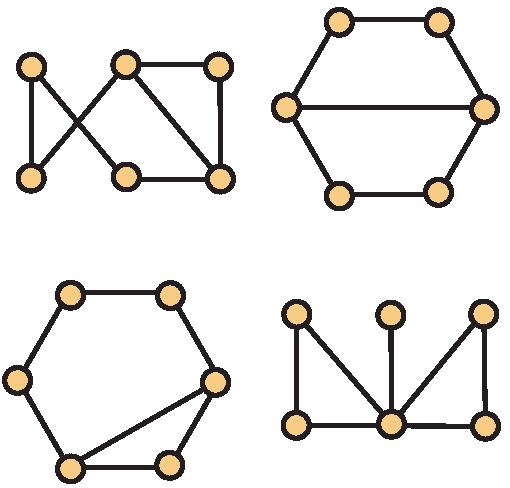
\includegraphics[width=\linewidth]{images/isomorphic_ex}
\end{image}%
\tcblower
\end{figureptx}%
\end{divisionexercise}%
\begin{divisionexercise}{4}{}{}{g:exercise:idp62}%
Let \(\bfG\) be a simple graph with \(n\) vertices and degree sequence \(a_1,a_2,\dots,a_n\).  What's the degree sequence of its complement \(\bfG^c\)?%
\end{divisionexercise}%
\begin{divisionexercise}{5}{}{}{g:exercise:idp63}%
Let \(G\) be the graph with graph with vertices consisting of the 10 three element subsets of \(\{a,b,c,d,e\}\), and two vertices adjacent if they share exactly one element.  So, for example, the two vertices \(v=\{a,c,e\}\) and \(w=\{b,c,d\}\) are adjacent, but neither \(v\) or \(w\) is adjacent to \(u=\{a,b,c\}\).%
\par
Draw \(G\) in a way that shows it is isomorphic to the Petersen graph.%
\par
Now let \(H\) be the graph with vertices consisting of the 10 \emph{two} element subsets of \(\{a,b,c,d,e\}\), and two vertices adjacent if they share \emph{no} elements.  Without drawing \(H\), write down an isomorphism between \(G\) and \(H\).  Hint: There's a "natural" bijection between the two and three element subsets of \(\{a,b,c,d,e\}\)%
\end{divisionexercise}%
\begin{divisionexercise}{6}{}{}{g:exercise:idp64}%
Recall that \(G^c\) denotes the complement of a graph \(G\).  Prove that \(f:G\to H\) is an isomorphism of graphs if and only if \(f:G^c\to H^c\) is an isomorphism.%
\end{divisionexercise}%
\begin{divisionexercise}{7}{}{}{g:exercise:idp65}%
Determine the number of non-isomorphic simple graphs with seven vertices such that each vertex has degree at least five.%
\par\smallskip%
\noindent\textbf{\blocktitlefont Hint}.\hypertarget{g:hint:idp66}{}\quad{}Consider the previous exercise%
\end{divisionexercise}%
\begin{divisionexercise}{8}{}{}{g:exercise:idp67}%
Consider the standard Instant Insanity puzzle, with four cubes and four colours.  Explain why one would expect there to be 331,776 different cube configurations.  Further explain why there would be fewer configurations if any cubes are coloured with symmetries.%
\par
In the text, we solve the puzzle by finding certain pairs of subgraphs.  Assuming that none of the cubes are coloured symmetrically, explain why each pair of subgraphs corresponds to at least 8 different cube configurations that are actually solutions, and why, depending on the isomorphism type of the subgraphs found, there may be more solutions.%
\end{divisionexercise}%
\begin{divisionexercise}{9}{}{}{g:exercise:idp68}%
Variations of the Insant Insanity puzzle increase the number of cubes and the number of colours.  Explain how to modify our graph theoretic solution to solve the puzzle when we have \(n\) cubes, each face of which is coloured one of \(n\) colours, and we want to line up the cubes so that each of the top, bottom, front and rear strings of cubes displays each of the \(n\) colours exactly once.%
\end{divisionexercise}%
\begin{divisionexercise}{10}{}{}{g:exercise:idp69}%
Use the method from the previous question to solve the following set of six cubes, marketed under the name "Drive ya crazy", where each face is coloured either blue, cyan, green, orange, red, or yellow.%
\begin{figureptx}{The six cubes from "Drive Ya crazy"}{x:figure:Driva_ya_crazy_cubes}{}%
\begin{image}{0.05}{0.9}{0.05}%
\resizebox{\linewidth}{!}{%
\begin{tikzpicture}[scale=.5]
\fill[cyan!50!white] (1,0) rectangle (2,1);
\fill[blue!50!white] (1,1) rectangle (2,2);
\fill[green] (1,2) rectangle (2,3);
\fill[yellow] (1,3) rectangle (2,4);
\fill[orange] (0,2) rectangle (1,3);
\fill[red!50!white] (2,2) rectangle (3,3);
\draw (1.5, .5) node {C};
\draw (1.5, 2.5) node {G};
\draw (1.5, 1.5) node {B};
\draw (2.5, 2.5) node {R};
\draw (1.5, 3.5) node {Y};
\draw (.5, 2.5) node {O};
\draw (1.5, -.5) node {Cube 1};


\draw (1,0) grid (2,4);
\draw (0,2) grid (3,3);

\begin{scope}[xshift=4cm]
\fill[blue!50!white] (1,0) rectangle (2,1);
\fill[green] (1,1) rectangle (2,2);
\fill[yellow] (1,2) rectangle (2,3);
\fill[orange] (1,3) rectangle (2,4);
\fill[red!50!white] (0,2) rectangle (1,3);
\fill[cyan!50!white] (2,2) rectangle (3,3);
\draw (1.5, .5) node {B};
\draw (1.5, 1.5) node {G};
\draw (1.5, 2.5) node {Y};
\draw (1.5, 3.5) node {O};
\draw (.5, 2.5) node {R};
\draw (2.5, 2.5) node {C};
\draw (1.5, -.5) node {Cube 2};

\draw (1,0) grid (2,4);
\draw (0,2) grid (3,3);
\end{scope}

\begin{scope}[xshift=8cm]
\fill[orange] (1,0) rectangle (2,1);
\fill[red!50!white] (1,1) rectangle (2,2);
\fill[cyan!50!white] (1,2) rectangle (2,3);
\fill[blue!50!white] (1,3) rectangle (2,4);
\fill[green] (0,2) rectangle (1,3);
\fill[yellow] (2,2) rectangle (3,3);
\draw (1.5, .5) node {O};
\draw (1.5, 1.5) node {R};
\draw (1.5, 2.5) node {C};
\draw (1.5, 3.5) node {B};
\draw (.5, 2.5) node {G};
\draw (2.5, 2.5) node {Y};
\draw (1.5, -.5) node {Cube 3};

\draw (1,0) grid (2,4);
\draw (0,2) grid (3,3);
\end{scope}

\begin{scope}[yshift=-6cm]
\fill[red!50!white] (1,0) rectangle (2,1);
\fill[cyan!50!white] (1,1) rectangle (2,2);
\fill[blue!50!white] (1,2) rectangle (2,3);
\fill[green] (1,3) rectangle (2,4);
\fill[yellow] (0,2) rectangle (1,3);
\fill[orange] (2,2) rectangle (3,3);
\draw (1.5, .5) node {R};
\draw (1.5, 1.5) node {C};
\draw (1.5, 2.5) node {B};
\draw (1.5, 3.5) node {G};
\draw (.5, 2.5) node {Y};
\draw (2.5, 2.5) node {O};
\draw (1.5, -.5) node {Cube 4};

\draw (1,0) grid (2,4);
\draw (0,2) grid (3,3);
\end{scope}

\begin{scope}[yshift=-6cm, xshift=4cm]
\fill[green] (1,0) rectangle (2,1);
\fill[yellow] (1,1) rectangle (2,2);
\fill[orange] (1,2) rectangle (2,3);
\fill[red!50!white] (1,3) rectangle (2,4);
\fill[cyan!50!white] (0,2) rectangle (1,3);
\fill[blue!50!white] (2,2) rectangle (3,3);
\draw (1.5, .5) node {G};
\draw (1.5, 1.5) node {Y};
\draw (1.5, 2.5) node {O};
\draw (1.5, 3.5) node {R};
\draw (.5, 2.5) node {C};
\draw (2.5, 2.5) node {B};
\draw (1.5, -.5) node {Cube 5};

\draw (1,0) grid (2,4);
\draw (0,2) grid (3,3);
\end{scope}

\begin{scope}[yshift=-6cm, xshift=8cm]
\fill[yellow] (1,0) rectangle (2,1);
\fill[orange] (1,1) rectangle (2,2);
\fill[red!50!white] (1,2) rectangle (2,3);
\fill[cyan!50!white] (1,3) rectangle (2,4);
\fill[blue!50!white] (0,2) rectangle (1,3);
\fill[green] (2,2) rectangle (3,3);
\draw (1.5, .5) node {Y};
\draw (1.5, 1.5) node {O};
\draw (1.5, 2.5) node {R};
\draw (1.5, 3.5) node {C};
\draw (.5, 2.5) node {B};
\draw (2.5, 2.5) node {G};
\draw (1.5, -.5) node {Cube 6};

\draw (1,0) grid (2,4);
\draw (0,2) grid (3,3);
\end{scope}

\end{tikzpicture}
}%
\end{image}%
\tcblower
\end{figureptx}%
\end{divisionexercise}%
\end{exercises-section}
\end{chapterptx}
%
%
\typeout{************************************************}
\typeout{Chapter 2 Walks}
\typeout{************************************************}
%
\begin{chapterptx}{Walks}{}{Walks}{}{}{x:chapter:ch_walks}
\begin{introduction}{}%
In this chapter we investigate walks in graphs.  We first look at some basic definitions and examples, we discuss Dijkstra's algorithm for finding the shortest path between two points in a weighted graph, and we discuss the notions of Eulerian and Hamiltonian graphs.%
\end{introduction}%
%
%
\typeout{************************************************}
\typeout{Section 2.1 Walks: the basics}
\typeout{************************************************}
%
\begin{sectionptx}{Walks: the basics}{}{Walks: the basics}{}{}{x:section:s_walks_basics}
If the edges in a graph \(\Gamma\) represent connections between different cities, it is obvious to strart planning longer trips that compose several of these connections.  The notion of a \emph{walk} formally captures this definition; the formal notions of \emph{path} and \emph{trail} further ask that we not double back on ourselves or repeat ourselves in certain formally defined ways.%
 \par
Once we've done that, we investigate what it means for a graph to be connected or disconnected.%
%
%
\typeout{************************************************}
\typeout{Subsection 2.1.1 Walks and connectedness}
\typeout{************************************************}
%
\begin{subsectionptx}{Walks and connectedness}{}{Walks and connectedness}{}{}{g:subsection:idp70}
Before we see the formal definition of a walk, it will be useful to see an example:%
\begin{figureptx}{Example of a walk}{x:figure:fig_walkdrawing}{}%
\begin{image}{0.15}{0.7}{0.15}%
\resizebox{\linewidth}{!}{%
\begin{tikzpicture}
\begin{scope}[every node/.style={circle,thick,draw}]
    \node (A) at (0,0) {A};
    \node (B) at (0,3) {B};
    \node (C) at (2.5,4) {C};
    \node (D) at (2.5,1) {D};
    \node (E) at (2.5,-3) {E};
    \node (F) at (5,3) {F} ;
\end{scope}

\begin{scope}[every node/.style={fill=white,circle}, >={Stealth[black]}]
  \begin{scope}[            
              every edge/.style={draw=red,very thick}]

  \path [->] (A) edge node {$6$} (D);
 \path [->] (D) edge node {$4$} (C);
    \path [->] (C) edge node {$5$} (F);
    \path [->] (F) edge node {$3$} (D);
    \path [->] (D) edge node {$8$} (E);
\end{scope}
    
    \path  (A) edge node {$3$} (B);
    \path  (B) edge node {$1$} (C); 
    \path  (A) edge node {$7$} (E);
    \path  (E) edge node {$9$} (F); 
    \path  (B) edge[bend right=60] node {$10$} (E); 
\end{scope}
\end{tikzpicture}
}%
\end{image}%
\tcblower
\end{figureptx}%
In the graph shown, the vertices are labelled with letters, and the edges are labelled with numbers, and we have a walk highlighted in red, and with arrowtips drawn on the edges.  Starting from vertex \(A\), we can take edge 6 to vertex \(D\), and then edge 5 to vertex \(C\), edge 5 to vertext \(F\), edge 3 back to vertex \(D\), and finally edge 8 to vertex \(E\). Intuitively,then, a walk strings together several edges that share vertices in between.  Makign that formal, we have the following.%
\begin{definition}{Walk.}{g:definition:idp71}%
\(walk\) in a graph \(\Gamma\) is a sequence%
%
\begin{equation*}
v_0, e_1, v_1,e_2, v_2,\dots, v_{n-1}, e_n, v_n
\end{equation*}
where the \(v_i\) are vertices, the \(e_j\) are edges, and the edge \(e_j\) goes between vertices \(v_{j-1}\) and \(v_j\).%
\par
We say that the walk is between vertices \(a=v_0\) and \(b=v_n\)%
\end{definition}
With this notation for a walk, Example \hyperref[x:figure:fig_walkdrawing]{Figure~{\xreffont\ref{x:figure:fig_walkdrawing}}}, the walk shown would be written \(A, 6, D, 4, C, 5, F, 3, D, 8, E\).  The visual representation of the walk on the graph is vastly more intuitive, the written one feeling cumbersome in comparison.%
\par
The definition of walk above contains some extra information.  If we just know the sequence of edges we can reconstruct what the vertices have to be (assuming we have at least two edges in the walk).  Alternatively, if the graph \(\Gamma\) does not have multiple edges, it is enough to just know the vertices \(v_i\), but if \(\Gamma\) has multiple edges that just knowing the vertices does not determine the walk.%
\begin{definition}{Connected.}{g:definition:idp72}%
We say a graph \(\Gamma\) is \emph{connected} if for any two vertices \(v,w\), there is a walk from \(v\) to \(w\) in \(\Gamma\).%
\end{definition}
\begin{definition}{Disjoint union.}{g:definition:idp73}%
Given two graphs \(\Gamma_1\) and \(\Gamma_2\), the \emph{disjoint union} \(\Gamma_1\sqcup \Gamma_2\) is obtained by taking the disjoint union of both the vertices and edges of \(\Gamma_1\) and \(\Gamma_2\).  So \(\Gamma_1\sqcup\Gamma_2\) consists of a copy of \(\Gamma_1\) and a copy of \(\Gamma_2\), with no edges in between the two graphs.%
\end{definition}
\begin{definition}{Disconnected.}{g:definition:idp74}%
A graph \(\Gamma\) is \emph{disconnected} if we can write \(\Gamma=\Gamma_1\sqcup \Gamma_2\) for two proper (i.e., not all of \(\Gamma\)) subgraphs \(\Gamma_1\) and \(\Gamma_2\).%
\end{definition}
We now have a definition for what it means for a graph to be connected, and another for what it means for a graph to be disconnected.  From everday usage of this words, we would certainly hope that a graph is disconnected if and only if it is not connected.  However, it is not immediately clear from the definitions as written that this is the case.%
\begin{lemma}{}{}{g:lemma:idp75}%
The following are equivalent:%
%
\begin{enumerate}
\item{}. \(\Gamma\) is connected%
\item{}\(\Gamma\) is not disconnected%
\end{enumerate}
\end{lemma}
\begin{proof}{}{g:proof:idp76}
1 implies 2: Supppose that \(\Gamma\) is connected, and let \(v, w\in V(\Gamma)\); we want to show that there is a walk from \(v\) to \(w\).%
\par
Define \(S\subset V(\Gamma)\) to be the set of all vertices \(u\in V(\Gamma)\) so that there is a walk from \(v\) to \(u\); we want to show that \(w\in S\).%
\par
First, observe that there are no edges from \(S\) to \(V(\Gamma)\setminus S\).  Suppose that \(e\) was an edge between \(a\in S\) and \(b\in\Gamma\setminus S\).  Since \(a\in S\), by the definition of \(S\) there is a walk \(v=v_0v_1v_2\cdots v_m=a\) from \(v\) to \(a\).  We can add the edge \(e\) to the end of the walk, to get a walk from \(v\) to \(b\), and hence by definition \(b\in S\).%
\par
Now suppose that \(w\notin S\).  Then \(S\) and \(V(\Gamma)\setminus S\) are both nonempty, and by the above there are no edges between them, and so \(\Gamma\) is not connected, a contradiction.%
\par
To prove 2 implies 1, we prove the contrapositive.  If \(\Gamma\) is not connected, then there are two vertices \(v,w\in V(\Gamma)\) so that there is no walk from \(v\) to \(w\).%
\par
Suppose that \(\Gamma=\Gamma_1\sqcup\Gamma_2\), and pick \(v\in V(\Gamma_1), w\in V(\Gamma_2)\).  Any walk from \(v\) to \(w\) starts in \(V(\Gamma_1)\) and ends in \(V(\Gamma_2)\), and so at some point there must be an edge from a vertex in \(\Gamma_1\) to a vertex in \(\Gamma_2\), but there are no such edges \(\square\)%
\end{proof}
\end{subsectionptx}
%
%
\typeout{************************************************}
\typeout{Subsection 2.1.2 Types of Walks}
\typeout{************************************************}
%
\begin{subsectionptx}{Types of Walks}{}{Types of Walks}{}{}{g:subsection:idp77}
Many questions in graph theory ask whether or not a walk of a certain type exists on a graph: we introduce some notation that will be needed for these questions.%
\begin{definition}{}{g:definition:idp78}%
We say a walk is \emph{closed} if it starts and ends on the same vertex; i.e., \(v_0=v_n\).  The \emph{length} of a walk is \(n\), the number of edges in it.  The \emph{distance} between two vertices \(v\) and \(w\) is the length of the shortest walk from \(v\) to \(w\), if one exists, and \(\infty\) if one does not exist.%
\end{definition}
It is sometimes convenient to have terminology for walks that don't backtrack on themselves:%
\begin{definition}{}{g:definition:idp79}%
%
\begin{enumerate}
\item{}If the edges \(e_i\) of the walk are all distinct, we call it a \emph{trail}%
\item{}If the vertices \(v_i\) of the walk are all distinct (except possibly \(v_0=v_m\)), we call the walk a \emph{path}.  The exception is to allow for the possibility of closed paths.%
\end{enumerate}
\end{definition}
\begin{lemma}{}{}{g:lemma:idp80}%
Let \(v,w\in V(\Gamma)\).  The following are equivalent:%
%
\begin{enumerate}
\item{}There is a walk from \(v\) to \(w\)%
\item{}There is a trail from \(v\) to \(w\)%
\item{}There is a path from \(v\) to \(w\).%
\end{enumerate}
\end{lemma}
As is often the case, the formal write-up of the proof makes something that can seem very easy intuitively look laborious, so it's worth anlysing it briefly for our example walk \(A-D-C-F-D-E\) from \hyperref[x:figure:fig_walkdrawing]{Figure~{\xreffont\ref{x:figure:fig_walkdrawing}}}.  This walk is not a path as it repeats the vertex \(D\); however, we may simply remove the triangle \(D-C-F-D\) from the walk to get the trail \(A-D-E\).  this idea is what works in general.%
\begin{proof}{}{g:proof:idp81}
It is immediate from the definitions that 3 implies 2 which implies 1, as any path is a trail, and any trail is a walk.%
\par
That 1 implies 3 is intuitively obvious: if you repeat a vertex, then you've visited someplace twice, and weren't taking the shortest route.  Let's make this argument mathematically precise.%
\par
Suppose we have a walk \(v=v_0,e_1,\dots, e_m, v_m=w\) that is not a path.  Then, we must repeat some vertex, say \(v_i=v_k\), with \(i\lt k\).  Then we can cut out all the vertices and edges between \(v_i\) and \(v_k\) to obtain a new walk%
%
\begin{equation*}
v=v_0,e_1, v_1,\dots, e_i, v_i=v_k, e_{k+1}, v_{k+1}, e_{k+2}, v_{k+2}, \dots, v_m
\end{equation*}
Since \(i \lt k \), the new walk is strictly shorter than our original walk.  Since the length of a walk is finite, if we iterate this process the result must eventually terminate.  That means all our vertices are distinct, and hence is a path.%
\end{proof}
\end{subsectionptx}
\end{sectionptx}
%
%
\typeout{************************************************}
\typeout{Section 2.2 Eulerian Walks}
\typeout{************************************************}
%
\begin{sectionptx}{Eulerian Walks}{}{Eulerian Walks}{}{}{x:section:s_walks_eulerian}
In this section we introduce the problem of Eulerian walks, often hailed as the origins of graph theroy. We will see that determining whether or not a walk has an Eulerian circuit will turn out to be easy; in contrast, the problem of determining whether or not one has a Hamiltonian walk, which seems very similar, will turn out to be very difficult.%
%
%
\typeout{************************************************}
\typeout{Subsection 2.2.1 The bridges of Konigsburg}
\typeout{************************************************}
%
\begin{subsectionptx}{The bridges of Konigsburg}{}{The bridges of Konigsburg}{}{}{g:subsection:idp82}
The city of Konigsberg (now Kaliningrad) was built on two sides of a river, near the site of two large islands.   The four sectors of the city were connected by seven bridges, as follows (picture from Wikipedia):%
\begin{figureptx}{The city of Konigsburg in Euler's time}{x:figure:bridges_konigsberg}{}%
\begin{image}{0.15}{0.7}{0.15}%
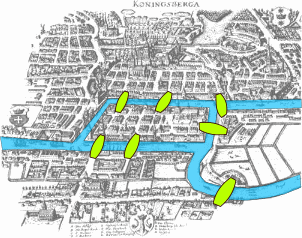
\includegraphics[width=\linewidth]{images/Konigsberg_bridges.png}
\end{image}%
\tcblower
\end{figureptx}%
A group of friends enjoyed strolling through the city, and created a game: could they take a walk in the city, crossing every bridge exactly once, and return to where they started from? They couldn't find such a walk, but they couldn't prove such a walk wasn't possible, and so they wrote to the mathematician Euler, who proved that such a walk is not possible.%
\end{subsectionptx}
%
%
\typeout{************************************************}
\typeout{Subsection 2.2.2 Eulerian Walks: definitions}
\typeout{************************************************}
%
\begin{subsectionptx}{Eulerian Walks: definitions}{}{Eulerian Walks: definitions}{}{}{g:subsection:idp83}
We will formalize the problem presented by the citizens of Konigsburg in graph theory, which will immediately present an obvious generalization.%
\par
We may represent the city of Konigsburg as a graph \(\Gamma_K\); the four sectors of town will be the vertices of \(\Gamma_K\), and edges between vertices will represent the bridges (hence, this will not be a simple graph).%
\par
Then, the question reduces to finding a closed walk in the graph that will uses every edge \emph{exactly} once. In particular, this walk will not use any edge more than once and hence will be a trail.%
\begin{inlineexercise}{}{g:exercise:idp84}%
\end{inlineexercise}%
\begin{definition}{}{g:definition:idp85}%
Let \(G\) be a graph.  An \emph{Eulerian cycle} is a closed walk that uses every edge of \(G\) exactly once.%
\par
If \(G\) has an Eulerian cycle, we say that \(G\) is \emph{Eulerian}.%
\par
If we weaken the requirement, and do not require the walk to be closed, we call it an Euler path, and if a graph \(G\) has an Eulerian path but not an Eulerian cycle, we say \(G\) is \emph{semi-Eulerian}%
\end{definition}
The question of the walkers of Konigsburg is then equivalent to asking if the graph \(\Gamma_K\) is Eulerian. The birth of graph theory is usually marked to the following theorem, proven by Euler:%
\begin{theorem}{}{}{x:theorem:thm_eulerian}%
A connected graph \(\Gamma\) is Eulerian if and only if every vertex of \(\Gamma\) has even degree%
\end{theorem}
\end{subsectionptx}
%
%
\typeout{************************************************}
\typeout{Subsection 2.2.3 A digression on proofs, formality, and intuition}
\typeout{************************************************}
%
\begin{subsectionptx}{A digression on proofs, formality, and intuition}{}{A digression on proofs, formality, and intuition}{}{}{g:subsection:idp86}
Before discussing the proof of \hyperref[x:theorem:thm_eulerian]{Theorem~{\xreffont\ref{x:theorem:thm_eulerian}}}, it's worth a little meta-discussion about proofs, intuition vs. rigor, and mathematics as a whole.  The proofing \hyperref[x:theorem:thm_eulerian]{Theorem~{\xreffont\ref{x:theorem:thm_eulerian}}} is a common exam question, and you may not be used to studying for reproducing proofs on exams.  Certainly one way to prepare for such a question is to memorize the proof word for word.  There doesn't seem to be a lot of obvious value in this approach, however.  So why ask these questions on the exam? And this opens the door to more philosophical questions as well: how should we think\slash{}interact with proofs anyway?  What's the point of it all?%
\par
Usually in books or in lectures, proofs are only given in slick, elegant, polished formal versions.  There are many reasons for this: there's a certain beauty to it; it's important to write it out formally to make sure it's all correct; there's only so much time in lectures, and brevity is a virtue anyway.  People turn away from long works, and the main point of a proof, after all, is to prove something, and it's easier to check that it's all correct if it's shorter.%
\par
But there's a very real downside to this presentation of proofs as the finished, elegant thing.  Most important to me is that the way mathematics is written formally on the page is very different from how it lives actively in our brains (or my brain, at least).  Nobody (or certainly very few people) comes up with proofs in the elegant short start to finish way that they're written.  Typically, there's a mess of chaotic half ideas that slowly get refined down to the written proof that you see.  But often the mess is the exciting part,%
\par
We sketch a few of the main ideas of the proof in an informal setting now, before giving a complete formal proof.  To learn this proof for the exam, you should have this informal picture in your head, and perhaps a skeleton outline of the main formal points that need to be shown.  You shouldn't try to memorize the formal proof word for word like a poem; instead, practice expanding out from the informal ideas\slash{}skeleton proof to the full formal proof on your own a few times.%
\par
It is much easier to see that if a graph \(G\) \emph{is} Eulerian, then every vertex has even degree.  Suppose we wanted to show that a given vertex \(v\) was Eulerian; let us stand at the vertex \(v\) and have a friend trace out the Eulerian cycle.  We'll wait for a while, and then the friend will appear at \(v\) along some edge \(e_1\), and then live along some different edge \(e_2\).  We'll wait some more, and they'll reappear coming from new edge \(e_3\), and then leave again along some edge \(e_4\).%
\par
This will continue until they have arrived or left by every edge that hits \(v\).  But every time they visit \(v\), they must arrive by one edge, and leave by another one, and hence every visit uses up an even number of edges, and so the degree \(d(v)\) of \(v\) must be even.  But there was nothing special about the vertex \(v\), and hence the degree of every vertex must be even.%
\par
To argue the other way is more difficult; before trying to show there's a closed path that uses all the edges, let's just construct \emph{any} closed path.  We pick some vertex \(v_0\) to start at, and just randomly choose an edge out of \(v_0\), to some other vertex \(v_1\), and from there randomly choosing any edge we haven't used yet to another vertex \(v_n\), and so on.%
\par
To construct a closed walk, we'd like to show we eventually have to return to \(v_0\).  We're only working with finite graphs, so our walk can't continue forever; the only possibility we have to rule out is that we reach some vertex \(v_n\) and find that we have already used every vertex incident to \(v_n\).  But as we saw before, the path will pair up the edges incident to each vertex as an arriving edge and a departing edge, and we know the degree of \(v_n\) is even.  If the path has already visited \(v_n k\) times, then we'll have used \(2k\) of the edges incident to it; when we arrive for the \(k+1\)st time we'll use one edge, and in all we'll have used \(2k+1\) edges, an odd number; since the degree of \(v_n\) is even there must be at least one edge we haven't used to exit by.%
\par
You might worry that the argument above suggests we can carry on the walk forever, which we obviously can't do since the graph is finite, but the argument above doesn't work for \(v_0\): when we start the path out at \(v_0\), we haven't had to arrive there, and so the edge we initially leave by is not paired with anything.  Therefore, if \(\Gamma\) has all vertices with even degree, and we walk randomly for as long as we can, we'll always get stuck at our starting vertex.%
\par
Hence, we have shown that if \(\Gamma\) is a graph with all vertices having even degree, there will exist some closed walk in \(\Gamma\), but the walk we created was chosen randomly, and there's no guarantee it will include all the edge of \(\Gamma\) -{}-{} in all likelihood, it won't.%
\par
But if we look at the edges we haven't used, they will form a simpler graph. \(\Gamma^\prime\).  There's no reason for \(\Gamma^\prime\) to be connected, but it's not too hard to see that every vertex of \(\Gamma^\prime\) will still have even degree: in \(\Gamma\) every vertex had even degree, and we saw in our first proof that a closed walk that doesn't repeat edges uses up an even number of edges at each vertex, and so we'll have an even number of edges left at each point.  Thus, each connected piece of \(\Gamma^\prime\) satisfies the hypothesis of the problem, and is simpler, so we can try to find a closed walk on each of connected piece of \(\Gamma^\prime\), and then "stitch" the results together to get a walk that uses all the pieces. In the formal proof, this process is best captured using induction, and we'll save the complete description until then, but for now we illustrate the process in an example%
\begin{figureptx}{Example of a walk}{x:figure:fig_walkdrawing_stupid}{}%
\begin{image}{0.15}{0.7}{0.15}%
\resizebox{\linewidth}{!}{%
\begin{tikzpicture}
\begin{scope}[every node/.style={circle,thick,draw}]
    \node (A) at (0,0) {A};
    \node (B) at (0,3) {B};
    \node (C) at (2.5,4) {C};
    \node (D) at (2.5,1) {D};
    \node (E) at (2.5,-3) {E};
    \node (F) at (5,3) {F} ;
\end{scope}

\begin{scope}[every node/.style={fill=white,circle}, >={Stealth[black]}]
  \begin{scope}[            
              every edge/.style={draw=red,very thick}]

  \path [->] (A) edge node {$6$} (D);
 \path [->] (D) edge node {$4$} (C);
    \path [->] (C) edge node {$5$} (F);
    \path [->] (F) edge node {$3$} (D);
    \path [->] (D) edge node {$8$} (E);
\end{scope}
    
    \path  (A) edge node {$3$} (B);
    \path  (B) edge node {$1$} (C); 
    \path  (A) edge node {$7$} (E);
    \path  (E) edge node {$9$} (F); 
    \path  (B) edge[bend right=60] node {$10$} (E); 
\end{scope}
\end{tikzpicture}
}%
\end{image}%
\tcblower
\end{figureptx}%
\begin{example}{}{g:example:idp87}%
Let's see an example of how the process of finding an Eulerian path works for the graph \(\Gamma\) in Figure below.%
\begin{figureptx}{A graph \(\Gamma\)}{x:figure:fig_euler_example}{}%
\begin{image}{0.15}{0.7}{0.15}%
\resizebox{\linewidth}{!}{%
\begin{tikzpicture}
\begin{scope}[scale=2]
\begin{scope}[every node/.style={circle, thick, draw}]
  \node (a) at (0,0) {$a$};
  \node (b) at (1,0) {$b$};
  \node (c) at (2,0) {$c$};
  \node (d) at (3,0) {$d$};
  \node (e) at (0,1) {$e$};
  \node (f) at (1,1) {$f$};
  \node (g) at (2,1) {$g$};
  \node (h) at (0,2) {$h$};
  \node (i) at (1,2) {$i$};
  \node (j) at (2,2) {$j$};
\end{scope}
\draw (a)--(e)--(h)--(i)--(f)--(e)--(i)--(j)--(g)--(c)--(d)--(g)--(b)--(a);
\end{scope}
\end{tikzpicture}
}%
\end{image}%
\tcblower
\end{figureptx}%
It probably isn't hard to immediately find an Eulerian cycle for \(\Gamma\) just by examination, but to illustrate the algorithm to begin with, we are going to deliberately choose a cycle that doesn't use every edge, the cycle aeijgba show in the next figure:%
\begin{figureptx}{Initializing with a closed walk in \(\Gamma\)}{x:figure:fig_euler_example_next}{}%
\begin{image}{0.15}{0.7}{0.15}%
\resizebox{\linewidth}{!}{%
\begin{tikzpicture}[scale=2]
\begin{scope}[every node/.style={circle, thick, draw}]
  \node (a) at (0,0) {$a$};
  \node (b) at (1,0) {$b$};
  \node (c) at (2,0) {$c$};
  \node (d) at (3,0) {$d$};
  \node (e) at (0,1) {$e$};
  \node (f) at (1,1) {$f$};
  \node (g) at (2,1) {$g$};
  \node (h) at (0,2) {$h$};
  \node (i) at (1,2) {$i$};
  \node (j) at (2,2) {$j$};
\end{scope}
\draw[thin, gray] (a)--(e)--(h)--(i)--(f)--(e)--(i)--(j)--(g)--(c)--(d)--(g)--(b)--(a);
\begin{scope}[every edge/.style={draw=red, very thick}, every node/.style={fill=white, circle}]
\path[->] (a) edge node {1} (e);
\path[->] (e) edge node {2} (i);
\path[->] (i) edge node {3} (j);
\path[->] (j) edge node {4} (g);
\path[->] (g) edge node {5} (b);
\path[->] (b) edge node {6} (a);
\end{scope}
\end{tikzpicture}
}%
\end{image}%
\tcblower
\end{figureptx}%
To extend our cycle to an Eulerian cycle, we delete all the edges used in the graph, and study the remaining graph.  In our case, this graph has two connected components, a four cycle and a three cycle.  Both of these are cycles themselves, they're trivially Eulerian, -{}-{} in general, it might take some work to find an Eulerian cycle for the components, but won't be too hard as the graph will be smaller.%
\begin{figureptx}{Parts of \(\Gamma\) missed by our walk}{x:figure:fig_euler_example_third}{}%
\begin{image}{0.15}{0.7}{0.15}%
\resizebox{\linewidth}{!}{%
\begin{tikzpicture}[scale=2]
\begin{scope}[every node/.style={circle, thick, draw}]


  \node (c) at (2,0) {$c$};
  \node (d) at (3,0) {$d$};
  \node (e) at (0,0) {$e$};
  \node (f) at (1,0) {$f$};
  \node (g) at (2,1) {$g$};
  \node (h) at (0,1) {$h$};
  \node (i) at (1,1) {$i$};
\end{scope}

\begin{scope}[every node/.style={fill=white, circle}]
\path[->] (e) edge node {1} (h);
\path[->] (h) edge node {2} (i);
\path[->] (i) edge node {3} (f);
\path[->] (f) edge node {4} (e);

\path[->] (g) edge node {1} (c);
\path[->] (c) edge node {2} (d);
\path[->] (d) edge node {3} (g);
\end{scope}

\end{tikzpicture}
}%
\end{image}%
\tcblower
\end{figureptx}%
Finally, we stitch our Eulerian paths together.  We follow our initial cycle that wasn't an Eulerian cycle, and the first time we hit a vertex that's in one of the other cycles, we insert that cycle in before we continue along our original path.  In our example, our original cycle was aeijgba.  a is not eitehr of the other components, but e is in the four cycle, so before we continue on our original cycle to i, we insert the four cycle ehije, giving aehije.  We now continue along our original cycle, adding ei, ij, jg, until we reach a vertex g that's in one of the added cycles, which we then insert, giving aehijeijgcdg as our cycle so far.%
\par
Continuing this process, we find aehijeijgcdgba as an Eulerian cycle.%
\begin{figureptx}{The Eulerian cycle stitched together}{x:figure:fig_euler_example_last}{}%
\begin{image}{0.15}{0.7}{0.15}%
\resizebox{\linewidth}{!}{%
\begin{tikzpicture}[scale=2]



\begin{scope}[every node/.style={circle, thick, draw}]
  \node (a) at (0,0) {$a$};
  \node (b) at (1,0) {$b$};
  \node (c) at (2,0) {$c$};
  \node (d) at (3,0) {$d$};
  \node (e) at (0,1) {$e$};
  \node (f) at (1,1) {$f$};
  \node (g) at (2,1) {$g$};
  \node (h) at (0,2) {$h$};
  \node (i) at (1,2) {$i$};
  \node (j) at (2,2) {$j$};
\end{scope}

\begin{scope}[every node/.style={fill=white, circle}]
\path[->] (a) edge node {1} (e);
\path[->] (e) edge node {2} (h);
\path[->] (h) edge node {3} (i);
\path[->] (i) edge node {4} (f);
\path[->] (f) edge node {5} (e);
\path[->] (e) edge node {6} (i);
\path[->] (i) edge node {7} (j);
\path[->] (j) edge node {8} (g);
\path[->] (g) edge node {9} (c);
\path[->] (c) edge node {10} (d);
\path[->] (d) edge node {11} (g);
\path[->] (g) edge node {12} (b);
\path[->] (b) edge node {13} (a);
\end{scope}

\end{tikzpicture}
}%
\end{image}%
\tcblower
\end{figureptx}%
\end{example}
\begin{proof}{}{g:proof:idp88}
We first show that if \(\bfG\) is Eulerian, then every vertex \(v\in\bfG\) has even degree.  For suppose the Eulerian cycle visits the vertex \(v k\) times.  Each time it visits \(v\) it must arrive by one edge, and leave by a different edge. Since the walk is Eulerian, every edge adjacent to \(v\) will be used exactly once by the walk, and so we see that \(d(v)=2k\) as desired.%
\par
Now we suppose that \(\bfG\) is connected and that every vertex has even degree.  We will induct on the number of edges of \(\bfG\).  If it has no edges, then the theorem is vacuously true -{}-{} we can just take the empty walk.%
\par
For the inductive step, suppose that \(\bfG\) is connected with \(m\) edges, and that every vertex of \(\bfG\) has even degree.  Further assume, for the inductive hypothesis, that every graph \(\bfH\) with these properties and \emph{less} than \(m\) edges is Eulerian.%
\par
Suppose for now that we can find \emph{a} closed walk \(w\) in \(\bfG\) that doesn't repeat any edges -{}-{} we will justify that this at the end of the proof.  If the closed walk \(w\) uses all the edges of \(\bfG\), then \(w\) is an Eulerian cycle, and we are done.%
\par
If \(w\) doesn't use all the edges of \(\bfG\), we can delete all the edges used in \(w\) and get a graph \(\bfG\setminus w\) with fewer than \(m\) edges.  Though \(\bfG\setminus w\) might not be connected, every vertex in \(\bfG\setminus w\) will have even degree, as we've subtracted an even number of edges from each vertex that \(w\) visits as argued in the first part of the proof.  Thus, by the inductive hypothesis each connected component \(\bfG\setminus w\) will have an Eulerian cycle.  Since the \(\bfG\) is connected, \(w\) must include at least one point from each component of \(\bfG\setminus w\), and so we can insert the Eulerian walk on the edges of each component of \(\bfG\setminus w\) from each component into \(w\) when we reach that component, to obtain a closed walk \(w^\prime\) that uses all the edges of \(\bfG\) exactly once, as desired.%
\par
All that remains is to justify that \(\bfG\) contains at least one closed walk, given that every vertex has even degree and it contains at least one edge.  We form a walk \(w\) by starting at any vertex \(v\) and at each step choosing any edge we've never traversed before at random as the next step of the walk.  We claim that \(w\) must eventually return back to the starting vertex \(v\).  Since \(\bfG\) is finite, and we don't repeat edges, the only way we could fail to return to \(v\) would be if our walk "got stuck" -{}-{} that is, at some point we reach a vertex \(u\) and find that every edge out of \(u\) has already been traversed.  However, we know that \(u\) has an even number of edges, and also arguing as in the first paragraph of the proof that every time the walk \(w\) visits \(u\) it must use up two edges, one for arrival and one for departure.  Hence, when we arrive at \(u\) at any time we must have used up an odd number of edges at \(u\) -{}-{} an even number from all the previous times we have visited \(u\), plus one more that we just arrived from.  Since \(u\) has even degree, there must always be at least one edge available for us to choose from, and so we can never "get stuck" and will eventually reach \(w\) again.%
\end{proof}
\begin{remark}{}{g:remark:idp89}%
Note that it does \emph{not} say: "A graph \(\Gamma\) is Eulerian if and only if it is connected and every vertex has even degree." This statement in quotation marks is false, but for "stupid" reasons.  If \(\Gamma\) is Eulerian, and \(E_n\) is the graph with \(n\) vertices wit no edges, then \(\Gamma\sqcup E_n\) is Eulerian but not connected.  These are the only examples of such graphs.%
\end{remark}
\begin{theorem}{}{}{g:theorem:idp90}%
A connected graph \(\Gamma\) is semi-Eulerian if and only if it has exactly two vertices with odd degree.%
\end{theorem}
\begin{proof}{}{g:proof:idp91}
A minor modification of our argument for Eulerian graphs shows that the condition is necessary.  Suppose that \(\Gamma\) is semi-Eulerian, with Eulerian path \(v_0, e_1, v_1,e_2,v_3,\dots,e_n,v_n\).  Then at any vertex other than the starting or ending vertices, we can pair the entering and leaving edges up to get an even number of edges.%
\par
However, at the first vertex \(v_0\) the path leaves along \(e_1\) the first time but never enters it accordingly, so that \(v_0\) has an odd degree; similarly, at \(v_n\) the path enters one final time along \(e_n\) without leaving, and so \(v_n\) also has an odd degree.%
\par
To see the condition is sufficient we could also modify the argument for the Eulerian case slightly, but it is slicker instead to \emph{reduce} to the Eulerian case.  Suppose that \(\Gamma\) is connected, and that vertices \(v\) and \(w\) have odd degree and all other vertices of \(\Gamma\) have even degree.  Then we can construct a new graph \(\Gamma^\prime\) by adding an extra edge \(e=vw\) to \(\Gamma\).  Then \(\Gamma^\prime\) is connected and every vertex has even degree, and so it has an Eulerian cycle.  Deleting the edge \(e\) that we added from this cycle gives an Eulerian path from \(v\) to \(w\) in \(\Gamma\).%
\end{proof}
\end{subsectionptx}
\end{sectionptx}
%
%
\typeout{************************************************}
\typeout{Section 2.3 Hamiltonian cycles}
\typeout{************************************************}
%
\begin{sectionptx}{Hamiltonian cycles}{}{Hamiltonian cycles}{}{}{x:section:s_walks_hamiltonian}
We now introduce the concept of Hamiltonian walks. Though on the surface the question seems very similar to determining whether or not a graph is Eulerian, it turns out to be much more difficult.%
\begin{definition}{}{g:definition:idp92}%
A graph is \emph{Hamiltonian} if it has a closed walk that uses every vertex exactly once; such a path is called a \emph{Hamiltonian cycle}%
\end{definition}
First, some very basic examples:%
%
\begin{enumerate}
\item{}The cycle graph \(C_n\) is Hamiltonian.%
\item{}Any graph obtained from \(C_n\) by adding edges is Hamiltonian%
\item{}The path graph \(P_n\) is \emph{not} Hamiltonian.%
\end{enumerate}
\begin{figureptx}{The Icosian game (from \href{https://www.puzzlemuseum.com/month/picm02/200207icosian.htm}{Puzzle Musuem}) and its solution (from \href{https://en.wikipedia.org/wiki/Icosian_game}{Wikipedia})}{x:figure:fig-icosian}{}%
\begin{sidebyside}{2}{0.05}{0.05}{0.1}%
\begin{sbspanel}{0.4}[center]%
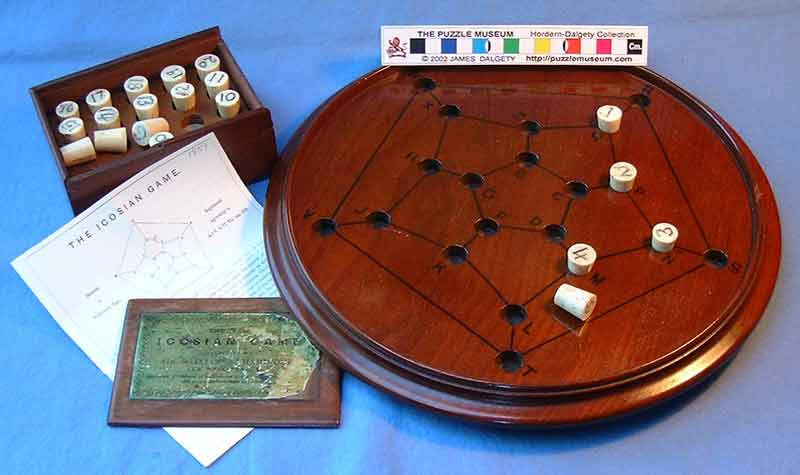
\includegraphics[width=\linewidth]{images/icosiangame.jpg}
\end{sbspanel}%
\begin{sbspanel}{0.4}[center]%
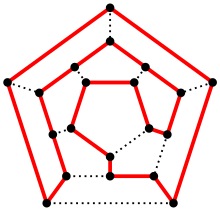
\includegraphics[width=\linewidth]{images/icosiansolved.png}
\end{sbspanel}%
\end{sidebyside}%
\tcblower
\end{figureptx}%
The term Hamiltonian comes from William Hamiltonian, who invented (a not very successful) board game he termed the "icosian game", which was about finding Hamiltonian cycles on the dodecahedron graph (and possibly its subgraphs).%
\par
The main thing you'll need to be able to do with Hamiltonian graphs is decide whether a given graph is Hamiltonian or not.  Although the definition of Hamiltonian graph is very similar to that of Eulerian graph, it turns out the two concepts behave very differently.  While Euler's Theorem gave us a very easy criterion to check to see whether or not a graph Eulerian, there is no such criterion to see if a graph is Hamiltonian or not.  It turns out that deciding whether or not a graph is Hamiltonian is NP-complete, meaning that if we could solve that problem efficiently, then you could solve a host of other difficult problems efficiently as well.%
\par
It may seem unfair, then, to ask whether a graph is Hamiltonian or not.  But it's only in a very theoretical way that the problem is extremely difficult -{}-{} as the number of vertices get very large, the problem gets harder and harderquickly.  For any given graph with a low number of vertices, there aren't that many possibilities to check.%
\par
If a graph \emph{is} Hamiltonian, then by far the best way to show it is to exhibit a Hamiltonian cycle, as in \hyperref[x:figure:fig-icosian]{Figure~{\xreffont\ref{x:figure:fig-icosian}}}.  When the graph isn't Hamiltonian, things become more interesting.%
\par
The most natural way to prove a graph isn't Hamiltonian is to do a case by case analysis of possible paths, showing it doesn't work.  For instance, in lecture we outlined the proof that if you remove a vertex from the Icosian graph, than the result isn't Hamiltonian.  A natural way to do this is to pick a vertex, and consider the possible pairs of edges the path might take through that vertex.  For each possibility, we know some edges won't be used, and can go further along that way.%
\par
In general, brute-force case-by-case analyses are proofs we want to avoid when possible, because it can be difficult to make sure we have actually found all the cases, and the proofs aren't always enlightening.  It's much better when we can find a "reason" why the graph isn't Hamiltonian.%
\begin{example}{}{g:example:idp93}%
\begin{figureptx}{A local configuration that can't exist in a Hamiltonian graph}{x:figure:figure-hamiltonian-obstruction}{}%
\begin{image}{0.15}{0.7}{0.15}%
\resizebox{\linewidth}{!}{%
\begin{tikzpicture}

\begin{scope}[every node/.style={circle,thick,draw}]
    \node (X) at (0,0) {X};
    \node (Y) at (2,0) {Y};
    \node (A) at (1,1) {A};
    \node (B) at (1, -1) {B};
\end{scope}

\draw (-1,,5)--(X)--(A)--(Y)--(3,.5);
\draw (-1,0)--(X)--(B)--(Y)--(3, -.5);
\draw (-1,-.5)--(X);

\end{tikzpicture}
}%
\end{image}%
\tcblower
\end{figureptx}%
\hyperref[x:figure:figure-hamiltonian-obstruction]{Figure~{\xreffont\ref{x:figure:figure-hamiltonian-obstruction}}} shows a portion of a larger graph \(\bfG\).  The exact number of other vertices in the graph that \(X\) and \(Y\) are adjacent to is not important; what matters is that \(A\) and \(B\) are each adjacent to two vertices, \(X\) and \(Y\).  Any path through \(A\) would have to use \(X\) and \(Y\), but so would any path through \(B\).  But then we have a small four cycle \(XAYBX\) which doesn't use any other vertices in the graph, and so \(\bfG\) cannot be HAmiltonian.%
\end{example}
\begin{lemma}{}{}{x:lemma:lemma-bipartite-hamiltonian}%
Suppose that \(\bfG\) is bipartite and Hamiltonian, with \(n\) red vertices and \(m\) blue vertices.%
\end{lemma}
\begin{proof}{}{g:proof:idp94}
Consider a Hamiltonian path in \(\bfG\).  Since every edge is between a red and blue vertex, the vertices in the path must alternate between red and blue.  Considering every other edge of the cycle pairs each red vertex with a blue vertex, and hence \(n=m\).%
\end{proof}
The contrapositive of \hyperref[x:lemma:lemma-bipartite-hamiltonian]{Lemma~{\xreffont\ref{x:lemma:lemma-bipartite-hamiltonian}}} can be used to show graphs \emph{aren't} Hamiltonian: if \(\bfG\) is bipartite but doesn't have the same number of red vertices and blue vertices, then it can't be Hamiltonian.%
\begin{lemma}{}{}{g:lemma:idp95}%
The Petersen Graph is not Hamiltonian%
\end{lemma}
\begin{proof}{}{g:proof:idp96}
Of course, a case-by-case analysis of possibile Hamiltonian cycles is possible.  The number of cases can be reduced by using symmetries of the Petersen graph. Instead, for variation and to illustrate a different proof technique, we will use another method.%
\par
Assume for contradiction that the Petersen graph is Hamiltonian, and draw the ten vertices \(v_1,v_2,\dots,v_{10}\) around the cycle.  The Hamiltonian cycle uses 10 of the 15 edges in the Petersen graph, and so there must be 5 more edges, with each vertex incident to one of them, as in the Petersen graph every vertex has degree 3.%
\par
Let's analyse where else the edge adjacent to \(v_1\) could go.  It can't go to \(v_1\) itself, as the Petersen graph has no loops, and it can't go to \(v_2\) or \(v_{10}\) as the Petersen graph has no multiple edges.  If it went to \(v_3\) or \(v_9\) it would make a three cycle, which the Petersen graph doesn't have, and if it went to \(v_4\) or \(v_7\), there'd be a four cycle.  Hence, the only options are \(v_1\) is adjacent to \(v_5, v_6\) or \(v_7\).  By reversing the direction of the Hamiltonian path, \(v_5\) and \(v_7\) are equivalent, and there are only two cases.%
\par
But the same analysis holds for every vertex: the extra edge at any vertex can either go to the opposite side of the circle, or be "off by one" and skip three vertices to either direction.%
\par
We now claim that not all the extra edges can go "directly across" -{}-{} there must be at least one edge that's off by one.  If all the extra edges went directly across, then \(v_1\) would go to \(v_6\), and \(v_2\) would go to \(v_7\), and \(v_1-v_6-v_7-v_2-v_1\) would be a 4 cycle.%
\par
Hence, without loss of generality we may assume that the extra edge at \(v_1\) is \(v_1-v_5\).  Let us then consider the extra edge at \(v_6\).  It can't go directly across, as that is \(v_1\) which already has its extra edge.  Hence it must be off by one, and go to either \(v_2\) or \(v_{10}\).  But either way we get a four cycle: either \(v_1-v_2-v_6-v_5-v_1\), or \(v_1-v_{10}-v_6-v_5-v_1\).  Hence, we have a contradiction, and the Petersen graph cannot be Hamiltonian.%
\end{proof}
Finally, Ore's Theorem, a positive result, giving conditions which guarantee that a graph has a Hamiltonian cycle.  First, a little bit of intuition.  If we take an edge to a Hamiltonian graph the result is still Hamiltonian, and the complete graphs \(K_n\) are Hamiltonian.  Thus, one might expect that a graph with "enough" edges is Hamiltonian.%
\par
The trick is in finding an interesting meaning of the word "enough".  Simply counting the number of edges does not give very interesting bounds on what "enough" means, however -{}-{} the complete graph has \(n(n-1)/2\) edges, but we can make it non-Hamiltonian by removing only \(n-2\) edges: simply pick a vertex \(v\) and remove all but one of the \(n-1\) edges coming out of \(v\); then \(v\) will now have degree 1, and hence the resulting graph cannot be Hamiltonian.%
\begin{theorem}{Ore's Theorem.}{}{g:theorem:idp97}%
Let \(\bfG\) be a simple graph with \(n\) vertices, and assume that whenever two distinct vertices \(v,w\) are not adjacent, we have \(d(v)+d(w)\geq n\).  Then \(\bfG\) is Hamiltonian.%
\end{theorem}
\begin{proof}{}{g:proof:idp98}
We will argue by contradiction, and begin by passing to a maximal counterexample.  Note that if \(\bfG\) satisfies the hypotheses, and we add an edge \(e\) to \(\bfG\) between two non-adjacent vertices \(v\) and \(w\), then the result will still satisfy the hypothesis.  Indeed, we've only increased the degree of some vertices.  So, we had a counterexample \(\bfG\) to Ore's Theorem, we could iteratively add edges to \(\bfG\) that didn't create Hamiltonian cycles, until we got a graph \(\bfG\) that satisfies the hypotheses of Ore's theorem, desn't have any Hamiltonian cycles, but if we add any edge \(e\) to \(\bfG\) the result \emph{is} Hamiltonian.%
\par
We now observe that such a \(\bfG\) must have a Hamiltonian \emph{path}: indeed, pick any edge \(e\) not in \(\bfG\) and add it to \(\bfG\).  THe resulting graph is by assumption Hamiltonian, and since \(\bfG\) wasn't Hamiltonian, the Hamiltonian cycle must contain the edge \(e\).  Deleting the edge \(e\) from the Hamiltonian cycle gives a Hamiltonian path in \(\bfG\).%
\par
Thus, let \(v_1-v_2-\cdots v_n\) be a Hamiltonian path in \(\bfG\).  We know \(v_1\) and \(v_n\) are not adjacent, as otherwise \(\bfG\) would be Hamiltonian.  Thus, since \(\bfG\) satisfies the hypothesis of Ore's theorem,  we know \(d(v_1)+d(v_n)\geq n\).  We already have one edge adjacent to \(v_1\), and one edge adjacent to \(v_n\), and so there must be at least \(n-2\) other edges adjacent to one or other of these vertices.  We will see that no matter how we add \(n-2\) edges to these two vertices, we will create a Hamiltonian cycle.%
\par
To see this, note there is ever an \(i\) with \(v_1\) adjacent to \(v_i\) and \(v_{i-1}\) adjacent to \(v_n\), then \(\bfG\) would have a Hamiltonian cycle: namely \(v_1-v_2-\cdots-v_{i-1}-v_n-v_{n-1}-\vdots v_i-v_1\).  Now, there are \(n-3\) different vertices we can add edges to \(v_1\) to, namely \(v_3-v_{n-1}\), and similarly there are \(n-3\) vertices we can add edges connecting \(v_n\) to, namely \(v_2, \dots v_{n-2}\).  We arrange these \(2(n-3)\) edges into a a grid with 2 rows and \(n-3\) columns, so that the two edges in each column are \(v_1-v_i\) and \(v_n-v_{i-1}\), a pair of edges that can form a Hamiltonian cycle as in the last paragraph.%
\par
As we need to add at least \(n-2\) edges, but we only have \(n-3\) columns, there must be at least one column that contains two edges by the pigeonhole principle, but then we can create a Hamiltonian cycle using those two edges and the edges in our Hamiltonian path.%
\end{proof}
Note that Ore's Theorem is \emph{not} an if and only if, and so Ore's Theorem cannot be used to prove that graphs \emph{aren't} Hamiltonian.  Indeed, there are plenty of graphs that are Hamiltonian but do not satisfy the hypotheses of Ore's Theorem.  For instance, the cycle graph \(C_n\) is Hamiltonian, but every vertex has degree 2, so if \(n\geq 5\) the hypotheses of Ore's Theorem are not satisfied.%
\par
We also highlight that the proof began by considering a maximal counterexample to Ore's Theorem, and considering maximal\slash{}minimal counterexamples is often a useful proof technique, as you the maximality\slash{}minimality gives you some extra structure to work with.%
\end{sectionptx}
%
%
\typeout{************************************************}
\typeout{Exercises 2.4 Exercises}
\typeout{************************************************}
%
\begin{exercises-section}{Exercises}{}{Exercises}{}{}{x:exercises:s_walks_exercises}
\begin{divisionexercise}{1}{}{}{g:exercise:idp99}%
The questions in this exercise pertain to the graph \(\bfG\) shown in \hyperref[x:figure:fig_graphs_graph_ex]{Figure~{\xreffont\ref{x:figure:fig_graphs_graph_ex}}}.%
\begin{sidebyside}{2}{0.0125}{0.0125}{0.025}%
\begin{sbspanel}{0.6}%
%
\begin{enumerate}[label=(\alph*)]
\item{}What is the degree of vertex \(8\)?%
\item{}What is the degree of vertex \(10\)?%
\item{}How many vertices of degree \(2\) are there in \(\bfG\)? List them.%
\item{}Find a cycle of length \(8\) in \(\bfG\).%
\item{}What is the length of a shortest path from \(3\) to \(4\)?%
\item{}What is the length of a shortest path from \(8\) to \(7\)?%
\item{}Find a path of length \(5\) from vertex \(4\) to vertex \(6\).%
\end{enumerate}
\end{sbspanel}%
\begin{sbspanel}{0.35}%
\begin{figureptx}{A graph}{x:figure:fig_graphs_graph_ex}{}%
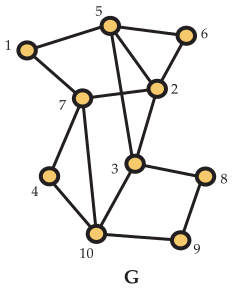
\includegraphics[width=\linewidth]{images/graph_ex}
\tcblower
\end{figureptx}%
\end{sbspanel}%
\end{sidebyside}%
\end{divisionexercise}%
\begin{divisionexercise}{2}{}{}{g:exercise:idp100}%
Draw a graph with \(8\) vertices, all of odd degree, that does not contain a path of length \(3\) or explain why such a graph does not exist.%
\end{divisionexercise}%
\begin{divisionexercise}{3}{}{}{g:exercise:idp101}%
Find an eulerian circuit in the graph \(\bfG\) in \hyperref[x:figure:fig_graphs_euler_exercise]{Figure~{\xreffont\ref{x:figure:fig_graphs_euler_exercise}}} or explain why one does not exist.%
\begin{figureptx}{A graph \(\bfG\)}{x:figure:fig_graphs_euler_exercise}{}%
\begin{image}{0.125}{0.75}{0.125}%
\resizebox{\linewidth}{!}{%
\begin{overpic}[width=4in]{images/euler_exercise}
                    \put(6,19.5){\(1\)}
                    \put(64.3,5){\(2\)}
                    \put(43.8,15){\(3\)}
                    \put(60,23.5){\(4\)}
                    \put(26,2){\(5\)}
                    \put(21,32){\(6\)}
                    \put(85,9){7}
                    \put(32.3,26.3){\(8\)}
                    \put(53,-1){\(9\)}
                    \put(42,33){\(10\)}
                    \put(71,26){\(11\)}
                    \put(83,21){\(12\)}
                    \end{overpic}
}%
\end{image}%
\tcblower
\end{figureptx}%
\end{divisionexercise}%
\begin{divisionexercise}{4}{}{}{g:exercise:idp102}%
Consider the graph \(\bfG\) in \hyperref[x:figure:fig_graphs_euler_hamilton_ex]{Figure~{\xreffont\ref{x:figure:fig_graphs_euler_hamilton_ex}}}. Determine if the graph is eulerian. If it is, find an eulerian circuit. If it is not, explain why it is not. Determine if the graph is hamiltonian. If it is, find a hamiltonian cycle. If it is not, explain why it is not.%
\begin{figureptx}{A graph \(\bfG\)}{x:figure:fig_graphs_euler_hamilton_ex}{}%
\begin{image}{0.175}{0.65}{0.175}%
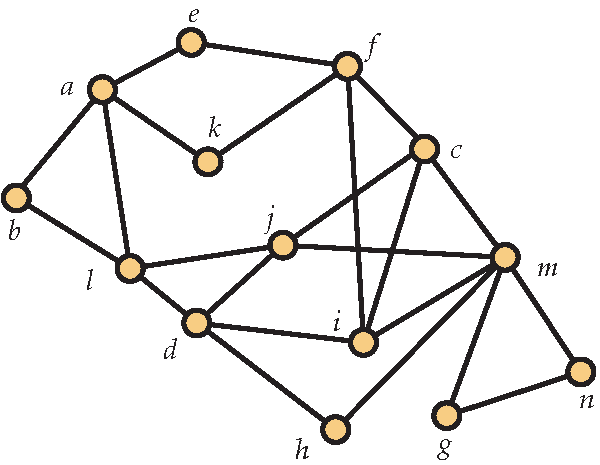
\includegraphics[width=\linewidth]{images/euler_hamilton_ex}
\end{image}%
\tcblower
\end{figureptx}%
\end{divisionexercise}%
\end{exercises-section}
\end{chapterptx}
%
%
\typeout{************************************************}
\typeout{Chapter 3 Algorithms}
\typeout{************************************************}
%
\begin{chapterptx}{Algorithms}{}{Algorithms}{}{}{x:chapter:ch_algorithms}
\begin{introduction}{}%
This chapter covers several graph algorithms.  We start with two algorithms for finding minimal weight spanning trees, Kruskal's algorithm and Prim's algorithm.  We discuss Dijkstra's algorithm for finding the shortest path between two points in a directed, weighted graph.%
\par
Much of the material in this chapter is taken from the open source textbook Applied Combinatorics by Keller and Trotter.%
\end{introduction}%
%
%
\typeout{************************************************}
\typeout{Section 3.1 Prüfer Codes}
\typeout{************************************************}
%
\begin{sectionptx}{Prüfer Codes}{}{Prüfer Codes}{}{}{x:section:s_graphalgorithms_prufer}
This section covers the Prüfer Code, a bijection between labelled trees and certain sequences of integers. This bijection allows us to prove Cayley's theorem, giving a count of such labelled trees.%
\par
Given a combinatorial structure, such as a graph or a tree, it is natural to ask how many of such structures there are.  Often, there is no nice formula, for instance, for the number of different trees on \(n\) vertices there.  But if the vertices are labelled, then it turns out there's a nice answer.%
\begin{definition}{Labelled tree.}{g:definition:idp103}%
A \emph{labelled tree} on \(n\) vertices is a tree with \(n\) vertices, which are labelled \(1,2,\dots,n.\)%
\end{definition}
\begin{theorem}{Cayley's Theorem.}{}{g:theorem:idp104}%
There are \(n^{n-2}\) labelled trees on \(n\) vertices.%
\end{theorem}
One more convenient way of writing down a labelled tree is to write down all the edges.  If there tree has \(n\) vertices, then there are \(n-1\) edges, and writing down all the edges takes \(2n-2\) numbers between \(1...n\).  However, we see that we're writing down the same tree lots of different times, by changing the order of the edges, and which vertex from each edge we write first.  Furthermore, not every sequence of \(2n-2\) numbers between \(1...n\) will result in a tree.%
\par
To fix this problem, we will write down the edges in a particular order.  Every tree has at least two leaves, and deleting a leaf gives a small tree.  We will use these facts to give a systematic ordering to the edges in a labelled tree, as follows: the first edge will be the edge connecting the leaf with the smallest label to the rest of the tree.  We will record that edge, with the leaf on the bottom row, and the "parent" vertex, i.e., the vertex the leaf is connected to, in the top row.  Deleting the leaf and the vertex gives a tree with one fewer vertex, and we iterate the process.%
\begin{algorithm}{Pruning Algorithm.}{}{g:algorithm:idp105}%
Input:  A labelled tree \(T\) on \(n\) vertices.%
\par
Output: A \(2\times n-1\) table with entries in \(\{1,\dots,n\}\) that records the edges of \(T\) in a specified order.%
Find the leaf \(v\) with the lowest label; it will have one edge \(e\), connecting it to some vertex (its "parent") \(w\).   Form a new tree \(T^\prime\) by deleting \(v\) and \(e\), and record \(e\) in the output table, putting the deleted vertex \(v\) in the bottom row and its parent \(w\) above it in the top row.%
\end{algorithm}
This method fixes the problem of the ordering of the edges not being unique, but as of now we are still recording more information than needed.  But note the following: since we delete a vertex when we put it in the bottom row, no number will appear twice on the bottom row.  The last column is the last two vertices existing, and if we look at the bottom row and the last entry on the top row, we see that every number from 1 to \(n\) will appear exactly once in these spots.%
\begin{definition}{Prüfer code.}{g:definition:idp106}%
If record the edges of a tree \(T\) as in the Pruning Algorithm, the first \(n-2\) number appear in the top row is the \emph{Prüfer code of \(T\)}%
\end{definition}
To finish the proof of Cayley's Theorem, we need to show that the Prüfer code is a bijection.  The easiest way to do this is to show that it has an inverse; that is, given any sequence of \(n-2\) numbers between 1 and \(n\), we can construct a tree \(T\) have that sequence as its Prüfer code.%
\par
This is most easily done by filling in the \(n\) numbers we deleted from the table of edges to get the Prüfer code.  We will in the numbers on the bottom row from left to right.  The first number on the bottom row will be the lowest number that does not appear in the Prüfer code.  Delete the first column, and then iterate -{}-{} the next number will be the lowest number we haven't used, and that doesn't appear in the remainder of the Prüfer code.%
\par
Another way to phrase the last line, is that the next number filled in is always the lowest number the doesn't appear as the bottom entry on one of the \(n-1\) columns.%
\begin{example}{}{g:example:idp107}%
Suppose \(T\) has Prüfer code 4,4,1,4,5,5. This code has length 6, so we looking to complete it by filling in numbers from 1 to 8. We illustrate the process step by step.%
\begin{sidebyside}{2}{0.025}{0.025}{0.05}%
\begin{sbspanel}{0.6}[center]%
The lowest number that doesn't appear is 2, so we fill that in on the bottom of the first column. We no longer have to consider the 4 directly above this 2, as it is not the bottom element of its column.%
\end{sbspanel}%
\begin{sbspanel}{0.3}[center]%
\begin{tableptx}{\textbf{}}{g:table:idp108}{}%
\resizebox{\linewidth}{!}{%
{\centering%
{\tabularfont%
\begin{tabular}{ccccccc}
\multicolumn{1}{cB}{4}&\multicolumn{1}{cB}{4}&\multicolumn{1}{cB}{1}&\multicolumn{1}{cB}{4}&\multicolumn{1}{cB}{5}&\multicolumn{1}{cB}{5}&\tabularnewline\hrulemedium
\multicolumn{1}{cB}{2}&\multicolumn{1}{cB}{}&\multicolumn{1}{cB}{}&\multicolumn{1}{cB}{}&\multicolumn{1}{cB}{}&\multicolumn{1}{cB}{}&
\end{tabular}
}%
\par}
}%
\end{tableptx}%
\end{sbspanel}%
\end{sidebyside}%
\begin{sidebyside}{2}{0.025}{0.025}{0.05}%
\begin{sbspanel}{0.6}[center]%
To fill in the next cell, we put the lowest number not occuring as the lowest element of a column, namely 3.%
\end{sbspanel}%
\begin{sbspanel}{0.3}[center]%
\begin{tableptx}{\textbf{}}{g:table:idp109}{}%
\resizebox{\linewidth}{!}{%
{\centering%
{\tabularfont%
\begin{tabular}{ccccccc}
\multicolumn{1}{cB}{4}&\multicolumn{1}{cB}{4}&\multicolumn{1}{cB}{1}&\multicolumn{1}{cB}{4}&\multicolumn{1}{cB}{5}&\multicolumn{1}{cB}{5}&\tabularnewline\hrulemedium
\multicolumn{1}{cB}{2}&\multicolumn{1}{cB}{3}&\multicolumn{1}{cB}{}&\multicolumn{1}{cB}{}&\multicolumn{1}{cB}{}&\multicolumn{1}{cB}{}&
\end{tabular}
}%
\par}
}%
\end{tableptx}%
\end{sbspanel}%
\end{sidebyside}%
\begin{sidebyside}{2}{0.025}{0.025}{0.05}%
\begin{sbspanel}{0.6}[center]%
And now the lowest term not on the bottom of its column is 6, so we add that:%
\end{sbspanel}%
\begin{sbspanel}{0.3}[center]%
\begin{tableptx}{\textbf{}}{g:table:idp110}{}%
\resizebox{\linewidth}{!}{%
{\centering%
{\tabularfont%
\begin{tabular}{ccccccc}
\multicolumn{1}{cB}{4}&\multicolumn{1}{cB}{4}&\multicolumn{1}{cB}{1}&\multicolumn{1}{cB}{4}&\multicolumn{1}{cB}{5}&\multicolumn{1}{cB}{5}&\tabularnewline\hrulemedium
\multicolumn{1}{cB}{2}&\multicolumn{1}{cB}{3}&\multicolumn{1}{cB}{6}&\multicolumn{1}{cB}{}&\multicolumn{1}{cB}{}&\multicolumn{1}{cB}{}&
\end{tabular}
}%
\par}
}%
\end{tableptx}%
\end{sbspanel}%
\end{sidebyside}%
\begin{sidebyside}{2}{0.025}{0.025}{0.05}%
\begin{sbspanel}{0.6}[center]%
Now the only 1 appearing has an element beneath it, and so 1 gets added in the next column:%
\end{sbspanel}%
\begin{sbspanel}{0.3}[center]%
\begin{tableptx}{\textbf{}}{g:table:idp111}{}%
\resizebox{\linewidth}{!}{%
{\centering%
{\tabularfont%
\begin{tabular}{ccccccc}
\multicolumn{1}{cB}{4}&\multicolumn{1}{cB}{4}&\multicolumn{1}{cB}{1}&\multicolumn{1}{cB}{4}&\multicolumn{1}{cB}{5}&\multicolumn{1}{cB}{5}&\tabularnewline\hrulemedium
\multicolumn{1}{cB}{2}&\multicolumn{1}{cB}{3}&\multicolumn{1}{cB}{6}&\multicolumn{1}{cB}{1}&\multicolumn{1}{cB}{}&\multicolumn{1}{cB}{}&
\end{tabular}
}%
\par}
}%
\end{tableptx}%
\end{sbspanel}%
\end{sidebyside}%
\begin{sidebyside}{2}{0.025}{0.025}{0.05}%
\begin{sbspanel}{0.6}[center]%
And now all the 4s have been passed, so the next number is 4.  We jump ahead and fill in the two numbers under 5 as well:%
\end{sbspanel}%
\begin{sbspanel}{0.3}[center]%
\begin{tableptx}{\textbf{}}{g:table:idp112}{}%
\resizebox{\linewidth}{!}{%
{\centering%
{\tabularfont%
\begin{tabular}{ccccccc}
\multicolumn{1}{cB}{4}&\multicolumn{1}{cB}{4}&\multicolumn{1}{cB}{1}&\multicolumn{1}{cB}{4}&\multicolumn{1}{cB}{5}&\multicolumn{1}{cB}{5}&\tabularnewline\hrulemedium
\multicolumn{1}{cB}{2}&\multicolumn{1}{cB}{3}&\multicolumn{1}{cB}{6}&\multicolumn{1}{cB}{1}&\multicolumn{1}{cB}{4}&\multicolumn{1}{cB}{7}&
\end{tabular}
}%
\par}
}%
\end{tableptx}%
\end{sbspanel}%
\end{sidebyside}%
\begin{sidebyside}{2}{0.025}{0.025}{0.05}%
\begin{sbspanel}{0.6}[center]%
The two numbers we haven't used yet are 5 and 8, so they are the entries in the last column, giving us the completed table of edges%
\end{sbspanel}%
\begin{sbspanel}{0.3}[center]%
\begin{tableptx}{\textbf{}}{g:table:idp113}{}%
\resizebox{\linewidth}{!}{%
{\centering%
{\tabularfont%
\begin{tabular}{ccccccc}
\multicolumn{1}{cB}{4}&\multicolumn{1}{cB}{4}&\multicolumn{1}{cB}{1}&\multicolumn{1}{cB}{4}&\multicolumn{1}{cB}{5}&\multicolumn{1}{cB}{5}&8\tabularnewline\hrulemedium
\multicolumn{1}{cB}{2}&\multicolumn{1}{cB}{3}&\multicolumn{1}{cB}{6}&\multicolumn{1}{cB}{1}&\multicolumn{1}{cB}{4}&\multicolumn{1}{cB}{7}&5
\end{tabular}
}%
\par}
}%
\end{tableptx}%
\end{sbspanel}%
\end{sidebyside}%
Having constructed the table encoding all the edges, we can now draw the labelled tree with those edges%
\begin{figureptx}{The tree with Prüfer code 441455}{x:figure:fig_pruferbackexample}{}%
\begin{image}{0.15}{0.7}{0.15}%
\resizebox{\linewidth}{!}{%
\begin{tikzpicture} 
\begin{scope}[scale=2, every node/.style={circle, thick, draw}]
    \node (1) at (0,0) {1};
    \node (6) at (0,1) {6};
    \node (4) at (1,0) {4};
    \node (2) at (1,1) {2};
    \node (5) at (2,0) {5};
    \node (3) at (2,1) {3};
    \node (7) at (3,0) {7};
    \node (8) at (3,1) {8};

\draw (6)--(1)--(4)--(5)--(7);
\draw (2)--(4)--(3);
\draw (5)--(8);
\end{scope}
\end{tikzpicture}
}%
\end{image}%
\tcblower
\end{figureptx}%
\end{example}
\end{sectionptx}
%
%
\typeout{************************************************}
\typeout{Section 3.2 Minimum Weight Spanning Trees}
\typeout{************************************************}
%
\begin{sectionptx}{Minimum Weight Spanning Trees}{}{Minimum Weight Spanning Trees}{}{}{x:section:s_graphalgorithms_min-wt-span}
\begin{introduction}{}%
In this section, we consider pairs \((\bfG,w)\) where \(\GVE\) is a connected graph and \(w\colon E\rightarrow\nonnegints\). For each edge \(e\in E\), the quantity \(w(e)\) is called the \terminology{weight}\index{weight} of \(e\). Given a set \(S\) of edges, we define the \terminology{weight} of \(S\), denoted \(w(S)\), by setting \(w(S)=\sum_{e\in S} w(e)\). In particular, the weight of a spanning tree \(T\) is just the sum of the weights of the edges in \(T\).\index{tree!spanning}%
\par
Weighted graphs arise in many contexts. One of the most natural is when the weights on the edges are distances or costs. For example, consider the weighted graph in \hyperref[x:figure:fig_graphalgorithms_spantreegraph]{Figure~{\xreffont\ref{x:figure:fig_graphalgorithms_spantreegraph}}}. Suppose the vertices represent nodes of a network and the edges represent the ability to establish direct physical connections between those nodes. The weights associated to the edges represent the cost (let's say in thousands of dollars) of building those connections. The company establishing the network among the nodes only cares that there is a way to get data between each pair of nodes. Any additional links would create redundancy in which they are not interested at this time. A spanning tree of the graph ensures that each node can communicate with each of the others and has no redundancy, since removing any edge disconnects it. Thus, to minimize the cost of building the network, we want to find a minimum weight (or cost) spanning tree.%
\begin{figureptx}{A weighted graph}{x:figure:fig_graphalgorithms_spantreegraph}{}%
\begin{image}{0.05}{0.9}{0.05}%
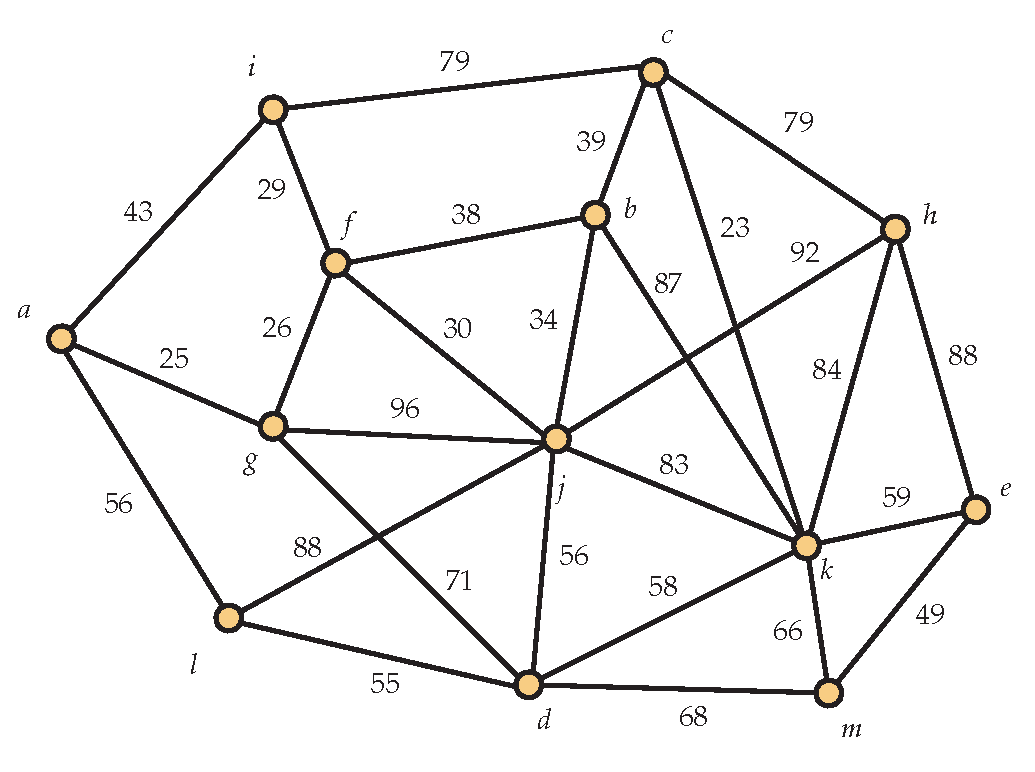
\includegraphics[width=\linewidth]{images/spantreegraph}
\end{image}%
\tcblower
\end{figureptx}%
To do this, this section considers the following problem:%
\begin{problem}{}{g:problem:idp114}%
Find a minimum weight spanning tree \(\bfT\) of \(\bfG\).%
\end{problem}
To solve this problem, we will develop \emph{two} efficient graph algorithms, each having certain computational advantages and disadvantages. Before developing the algorithms, we need to establish some preliminaries about spanning trees and forests.%
\end{introduction}%
%
%
\typeout{************************************************}
\typeout{Subsection 3.2.1 Preliminaries}
\typeout{************************************************}
%
\begin{subsectionptx}{Preliminaries}{}{Preliminaries}{}{}{g:subsection:idp115}
The following proposition about the number of components in a spanning forest of a graph \(\bfG\) has an easy inductive proof. You are asked to provide it in the exercises.%
\begin{proposition}{}{}{x:proposition:prop_graphalgorithms_spanforest}%
Let \(\GVE\) be a graph on \(n\) vertices, and let \(\bfH=(V,S)\) be a spanning forest. Then \(0\le |S|\le n-1\). Furthermore, if \(|S|= n-k\), then \(\bfH\) has \(k\) components. In particular, \(\bfH\) is a spanning tree if and only if it contains \(n-1\) edges.%
\end{proposition}
The following proposition establishes a way to take a spanning tree of a graph, remove an edge from it, and add an edge of the graph that is not in the spanning tree to create a new spanning tree. Effectively, the process exchanges two edges to form the new spanning tree, so we call this the \terminology{exchange principle}.%
\begin{proposition}{Exchange Principle.}{}{x:proposition:prop_graphalgorithms_exchange}%
Let \(\bfT=(V,S)\) be spanning tree in a graph \(\bfG\), and let \(e=xy\) be an edge of \(\bfG\) which does not belong to \(\bfT\). Then%
\begin{enumerate}
\item{}There is a \emph{unique} path \(P=(x_0,x_1,x_2,\dots,x_t)\) with (a)~\(x=x_0\); (b)~\(y=x_t\); and (c)~\(x_ix_{i+1}\in S\) for each \(i=0,1,2,\dots,t-1\).%
\item{}For each \(i=0,1,2,\dots,t-1\), let \(f_i=x_ix_{i+1}\) and then set%
\begin{equation*}
S_i = \{e\}\cup\{g\in S: g\neq f_i\},
\end{equation*}
i.e.\@, we \terminology{exchange} edge \(f_i\) for edge \(e\). Then \(\bfT_i=(V,S_i)\) is a spanning tree of \(\bfG\).%
\end{enumerate}
%
\end{proposition}
\begin{proof}{}{g:proof:idp116}
For the first fact, it suffices to note that if there were more than one distinct path from \(x\) to \(y\) in \(\bfT\), we would be able to find a cycle in \(\bfT\). This is impossible since it is a tree. For the second, we refer to \hyperref[x:figure:fig_graphalgorithms_exchange]{Figure~{\xreffont\ref{x:figure:fig_graphalgorithms_exchange}}}. The black and green edges in the graph shown at the left represent the spanning tree \(\bfT\). Thus, \(f\) lies on the unique path from \(x\) to \(y\) in \(\bfT\) and \(e=xy\) is an edge of \(\bfG\) \emph{not} in \(\bfT\). Adding \(e\) to \(\bfT\) creates a graph with a unique cycle, since \(\bfT\) had a unique path from \(x\) to \(y\). Removing \(f\) (which could be any edge \(f_i\) of the path, as stated in the proposition) destroys this cycle. Thus \(\bfT_i\) is a connected acyclic subgraph of \(\bfG\) with \(n-1+1-1=n-1\) edges, so it is a spanning tree.%
\begin{figureptx}{The exchange principle}{x:figure:fig_graphalgorithms_exchange}{}%
\begin{sidebyside}{2}{0.01}{0.01}{0.02}%
\begin{sbspanel}{0.48}%
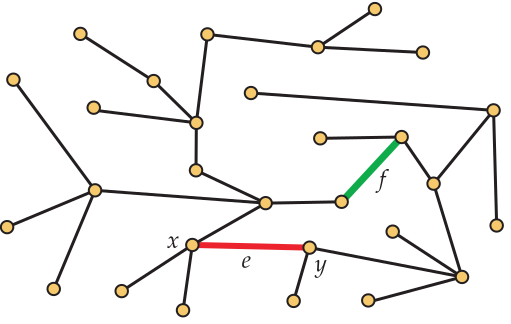
\includegraphics[width=\linewidth]{images/exchange1}
\end{sbspanel}%
\begin{sbspanel}{0.48}%
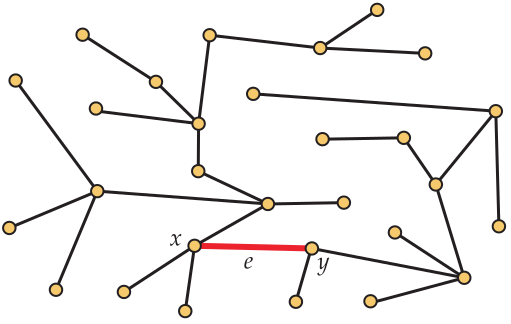
\includegraphics[width=\linewidth]{images/exchange2}
\end{sbspanel}%
\end{sidebyside}%
\tcblower
\end{figureptx}%
\end{proof}
For both of the algorithms we develop, the argument to show that the algorithm is optimal rests on the following technical lemma. To avoid trivialities, we assume \(n\ge3\).%
\begin{lemma}{}{}{x:lemma:lem_graphalgorithms_tech}%
Let \(\bfF\) be a spanning forest of \(\bfG\) and let \(C\) be a component of \(\bfF\). Also, let \(e=xy\) be an edge of minimum weight among all edges with one endpoint in \(C\) and the other not in \(C\). Then among all spanning trees of \(\bfG\) that contain the forest \(\bfF\), there is one of minimum weight that contains the edge \(e\).%
\end{lemma}
\begin{proof}{}{g:proof:idp117}
Let \(\bfT=(V,S)\) be any spanning tree of minimum weight among all spanning trees that contain the forest \(\bfF\), and suppose that \(e=xy\) is not an edge in \(\bfT\). (If it were an edge in \(\bfT\), we would be done.) Then let \(P=(x_0,x_1,x_2,\dots,x_t)\) be the unique path in \(\bfT\) with (a)~\(x=x_0\); (b)~\(y=x_t\); and (c)~\(x_ix_{i+1}\in S\) for each \(i=0,1,2,\dots,t-1\). Without loss of generality, we may assume that \(x=x_0\) is a vertex in \(C\) while \(y=x_t\) does not belong to \(C\). Then there is a least non-negative integer \(i\) for which \(x_i\) is in \(C\) and \(x_{i+1}\) is not in \(C\). It follows that \(x_j\) is in \(C\) for all \(j\) with \(0\le j\le i\).%
\par
Let \(f=x_ix_{i+1}\). The edge \(e\) has minimum weight among all edges with one endpoint in \(C\) and the other not in \(C\), so \(w(e)\le w(f)\). Now let \(\bfT_i\) be the tree obtained by exchanging the edge \(f\) for edge~\(e\). It follows that \(w(\bfT_i) = w(\bfT) - w(f) +w(e)\le w(\bfT)\). Furthermore, \(\bfT_i\) contains the spanning forest \(\bfF\) as well as the edge~\(e\). It is therefore the minimum weight spanning tree we seek.%
\end{proof}
\begin{remark}{}{g:remark:idp118}%
Although Bob's combinatorial intuition has improved over the course he doesn't quite understand why we need special algorithms to find minimum weight spanning trees. He figures there can't be that many spanning trees, so he wants to just write them down. Alice groans as she senses that Bob must have been absent when the material from \hyperref[x:section:s_graphalgorithms_prufer]{Section~{\xreffont\ref{x:section:s_graphalgorithms_prufer}}} was discussed. In that section, we learned that a graph on \(n\) vertices can have as many as \(n^{n-2}\) spanning trees (or horrors, the instructor may have left it off the syllabus). Regardless, this exhaustive approach is already unusable when \(n = 20\). Dave mumbles something about being greedy and just adding the lightest edges one-by-one while never adding an edge that would make a cycle. Zori remembers a strategy like this working for finding the height of a poset, but she's worried about the nightmare situation that we learned about with using FirstFit to color graphs. Alice agrees that greedy algorithms have an inconsistent track record but suggests that \hyperref[x:lemma:lem_graphalgorithms_tech]{Lemma~{\xreffont\ref{x:lemma:lem_graphalgorithms_tech}}} may be enough to get one to succeed here.%
\end{remark}
\end{subsectionptx}
%
%
\typeout{************************************************}
\typeout{Subsection 3.2.2 Kruskal's Algorithm}
\typeout{************************************************}
%
\begin{subsectionptx}{Kruskal's Algorithm}{}{Kruskal's Algorithm}{}{}{g:subsection:idp119}
In this section, we develop one of the best known algorithms for finding a minimum weight spanning tree. It is known as \terminology{Kruskal's Algorithm}, although some prefer the descriptive label \emph{Avoid Cycles} because of the way it builds the spanning tree.%
\par
To start Kruskal's algorithm, we sort the edges according to weight.  To be more precise, let \(m\) denote the number of edges in \(\GVE\).  Then label the edges as \(e_1,e_2,e_3,\dots,e_m\) so that \(w(e_1)\le w(e_2)\le \dots \le w(e_m)\). Any of the many available efficient sorting algorithms can be used to do this step.%
\par
Once the edges are sorted, Kruskal's algorithm proceeds to an initialization step and then inductively builds the spanning tree \(\bfT=(V,S)\):%
\begin{algorithm}{Kruskal's Algorithm.}{}{x:algorithm:alg_kruskal}%
\index{minimum weight spanning tree!Kruskal's algorithm for}%
\index{Kruskal's algorithm}%
%
\begin{description}
\item[{Initialization.}]Set \(S=\emptyset\) and \(i=0\).%
\item[{Inductive Step.}]While \(|S| \lt n-1\), let \(j\) be the least non-negative integer so that \(j > i\) and there are no cycles in \(S\cup\{e_j\}\). Then (using pseudo-code) set%
\begin{equation*}
i = j\quad\text{and} \quad S= S\cup\{j\}.
\end{equation*}
%
\end{description}
%
\end{algorithm}
The correctness of Kruskal's Algorithm follows from an inductive argument. First, the set \(S\) is initialized as the empty set, so there is certainly a minimum weight spanning tree containing all the edges in \(S\). Now suppose that for some \(i\) with \(0\le i \lt n\), \(|S|=i\) and there is a minimum weight spanning tree containing all the edges in \(S\). Let \(\bfF\) be the spanning forest determined by the edges in \(S\), and let \(C_1, C_2,\dots,C_s\) be the components of \(\bfF\). For each \(k=1,2,\dots,s\), let \(f_k\) be a minimum weight edge with one endpoint in \(C_k\) and the other not in \(C_k\). Then the edge \(e\) added to \(S\) by Kruskal's Algorithm is just the edge \(\{f_1,f_2,\dots,f_s\}\) having minimum weight. Applying \hyperref[x:lemma:lem_graphalgorithms_tech]{Lemma~{\xreffont\ref{x:lemma:lem_graphalgorithms_tech}}} and the inductive hypothesis, we know that there will still be a minimum weight spanning tree of \(\bfG\) containing all the edges of \(S\cup\{e\}\).%
\begin{example}{Kruskal's Algorithm.}{g:example:idp120}%
\begin{sidebyside}{2}{0.0125}{0.0125}{0.025}%
\begin{sbspanel}{0.78}%
Let's see what Kruskal's algorithm does on the weighted graph in \hyperref[x:figure:fig_graphalgorithms_spantreegraph]{Figure~{\xreffont\ref{x:figure:fig_graphalgorithms_spantreegraph}}}.  It first sorts all of the edges by weight. We won't reproduce the list here, since we won't need all of it. The edge of least weight is \(ck\), which has weight \(23\). It continues adding the edge of least weight, adding \(ag\), \(fg\), \(fi\), \(fj\), and \(bj\). However, after doing this, the edge of lowest weight is \(fb\), which has weight \(38\). This edge cannot be added, as doing so would make \(fjb\) a cycle. Thus, the algorithm bypasses it and adds \(bc\). Edge \(ai\) is next inspected, but it, too, would create a cycle and is eliminated from consideration. Then \(em\) is added, followed by \(dl\). There are now \emph{two} edges of weight \(56\) to be considered: \(al\) and \(dj\). Our sorting algorithm has somehow decided one of them should appear first, so let's say it's \(dj\). After adding \(dj\), we cannot add \(al\), as \(agfjdl\) would form a cycle. Edge \(dk\) is next considered, but it would also form a cycle. However, \(ek\) can be added. Edges \(km\) and \(dm\) are then bypassed. Finally, edge \(ch\) is added as the twelfth and final edge for this \(13\)-vertex spanning tree. The full list of edges added (in order) is shown to the right. The total weight of this spanning tree is \(504\).%
\end{sbspanel}%
\begin{sbspanel}{0.17}%
\begin{preformatted}
c k 23
a g 25
f g 26
f i 29
f j 30
b j 34
b c 39
e m 49
d l 55
d j 56
e k 59
c h 79
\end{preformatted}
\end{sbspanel}%
\end{sidebyside}%
\end{example}
\end{subsectionptx}
%
%
\typeout{************************************************}
\typeout{Subsection 3.2.3 Prim's Algorithm}
\typeout{************************************************}
%
\begin{subsectionptx}{Prim's Algorithm}{}{Prim's Algorithm}{}{}{x:subsection:alg_prim}
We now develop \terminology{Prim's Algorithm} for finding a minimum weight spanning tree. This algorithm is also known by a more descriptive label: \emph{Build Tree}. We begin by choosing a root vertex \(r\). Again, the algorithm proceeds with an initialization step followed by a series of inductive steps.%
\begin{algorithm}{Prim's Algorithm.}{}{g:algorithm:idp121}%
\index{minimum weight spanning trees!Prim's algorithm for}%
\index{Prim's algorithm}%
%
\begin{description}
\item[{Initialization.}]Set \(W=\{r\}\) and \(S=\emptyset\).%
\item[{Inductive Step.}]While \(|W| \lt n\), let \(e\) be an edge of minimum weight among all edges with one endpoint in \(W\) and the other not in \(W\).  If \(e=xy\), \(x\in W\) and \(y\not\in W\), update \(W\) and \(S\) by setting (using pseudo-code)%
\begin{equation*}
W = W\cup\{y\}\quad\text{and} \quad S = S\cup\{e\}.
\end{equation*}
%
\end{description}
%
\end{algorithm}
The correctness of Prim's algorithm follows immediately from \hyperref[x:lemma:lem_graphalgorithms_tech]{Lemma~{\xreffont\ref{x:lemma:lem_graphalgorithms_tech}}}.%
\begin{example}{Prim's Algorithm.}{g:example:idp122}%
\begin{sidebyside}{2}{0.0125}{0.0125}{0.025}%
\begin{sbspanel}{0.78}%
Let's see what Prim's algorithm does on the weighted graph in \hyperref[x:figure:fig_graphalgorithms_spantreegraph]{Figure~{\xreffont\ref{x:figure:fig_graphalgorithms_spantreegraph}}}. We start with vertex \(a\) as the root vertex. The lightest edge connecting \(a\) (the only vertex in the tree so far) to the rest of the graph is \(ag\). Next, \(fg\) is added. This is followed by \(fi\), \(fj\), \(bj\), and \(bc\). Next, the algorithm identifies \(ck\) as the lightest edge connecting \(\{a,g,i,f,j,b,c\}\) to the remaining vertices. Notice that this is considerably later than Kruskal's algorithm finds the same edge. The algorithm then determines that \(al\) and \(jd\), both of weight \(56\) are the lightest edges connecting vertices in the tree to the other vertices. It picks arbitrarily, so let's say it takes \(al\). It next finds \(dl\), then \(ek\), and then \(em\). The final edge added is \(ch\). The full list of edges added (in order) is shown to the right. The total weight of this spanning tree is \(504\). This (not surprisingly) the same weight we obtained using Kruskal's algorithm. However, notice that the spanning tree found is different, as this one contains \(al\) instead of \(dj\). This is not an issue, of course, since in both cases an arbitrary choice between two edges of equal weight was made.%
\end{sbspanel}%
\begin{sbspanel}{0.17}%
\begin{preformatted}
a g 25
f g 26
f i 29
f j 30
b j 34
b c 39
c k 23
a l 56
d l 55
e k 59
e m 49
c h 79
\end{preformatted}
\end{sbspanel}%
\end{sidebyside}%
\end{example}
\end{subsectionptx}
%
%
\typeout{************************************************}
\typeout{Subsection 3.2.4 Comments on Efficiency}
\typeout{************************************************}
%
\begin{subsectionptx}{Comments on Efficiency}{}{Comments on Efficiency}{}{}{g:subsection:idp123}
An implementation of Kruskal's algorithm seems to require that the edges be sorted. If the graph has \(n\) vertices and \(m\) edges, this requires \(m\log m\) operations just for the sort. But once the sort is done, the process takes only \(n-1\) steps\textemdash{}provided you keep track of the components as the spanning forest expands.  Regardless, it is easy to see that at most \(O(n^2\log n)\) operations are required.%
\par
On the other hand, an implementation of Prim's algorithm requires the program to conveniently keep track of the edges incident with each vertex and always be able to identify the edge with least weight among subsets of these edges. In computer science, the data structure that enables this task to be carried out is called a \terminology{heap}.%
\end{subsectionptx}
\end{sectionptx}
%
%
\typeout{************************************************}
\typeout{Section 3.3 Digraphs}
\typeout{************************************************}
%
\begin{sectionptx}{Digraphs}{}{Digraphs}{}{}{x:section:s_graphalgorithms_digraphs}
In this section, we introduce another useful variant of a graph. In a graph, the existence of an edge \(xy\) can be used to model a connection between \(x\) and \(y\) that goes in both ways. However, sometimes such a model is insufficient. For instance, perhaps it is possible to fly from Atlanta directly to Fargo but not possible to fly from Fargo directly to Atlanta. In a graph representing the airline network, an edge between Atlanta and Fargo would lose the information that the flights only operate in one direction. To deal with this problem, we introduce a new discrete structure. A \terminology{digraph}\index{digraph}\index{graph!directed|see{digraph}} \(\bfG\) is a pair \((V,E)\) where \(V\) is a vertex set and \(E\subset V\times V\) with \(x\neq y\) for every \((x,y)\in E\). We consider the pair \((x,y)\) as a \terminology{directed edge}\index{edge!directed} from \(x\) to \(y\). Note that for distinct vertices \(x\) and \(y\) from \(V\), the ordered pairs \((x,y)\) and \((y,x)\) are distinct, so the digraph may have one, both or neither of the directed edges \((x,y)\) and \((y,x)\). This is in contrast to graphs, where edges are sets, so \(\{x,y\}\) and \(\{y,x\}\) are the same.%
\par
Diagrams of digraphs use arrowheads on the edges to indicate direction.  This is illustrated in \hyperref[x:figure:fig_graphalgorithms_digraph]{Figure~{\xreffont\ref{x:figure:fig_graphalgorithms_digraph}}}. For example, the digraph illustrated there contains the edge \((a,f)\) but not the edge \((f,a)\). It does contain both edges \((c,d)\) and \((d,c)\), however.%
\begin{figureptx}{A Digraph}{x:figure:fig_graphalgorithms_digraph}{}%
\begin{image}{0.075}{0.85}{0.075}%
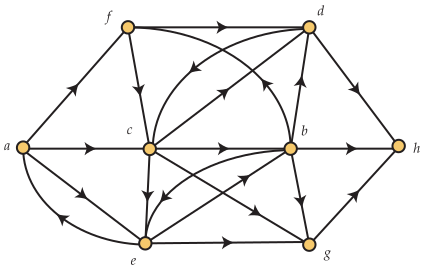
\includegraphics[width=\linewidth]{images/digraph}
\end{image}%
\tcblower
\end{figureptx}%
When \(\bfG\) is a digraph, a sequence \(P=(r=u_0,u_1,\dots,u_t=x)\) of distinct vertices is called a \terminology{directed path}\index{path!directed} from \(r\) to \(x\) when \((u_iu_{i+1})\) is a directed edge in \(\bfG\) for every \(i=0,1,\dots,t-1\). A directed path \(C=(r=u_0,u_1,\dots,u_t=x)\) is called a \terminology{directed cycle}\index{cycle!directed} when \((u_t,u_0)\) is a directed edge of \(\bfG\).%
\end{sectionptx}
%
%
\typeout{************************************************}
\typeout{Section 3.4 Dijkstra's Algorithm for Shortest Paths}
\typeout{************************************************}
%
\begin{sectionptx}{Dijkstra's Algorithm for Shortest Paths}{}{Dijkstra's Algorithm for Shortest Paths}{}{}{x:section:s_graphalgorithms_shortest-paths}
\begin{introduction}{}%
Just as with graphs, it is useful to assign weights to the directed edges of a digraph. Specifically, in this section we consider a pair \((\bfG,w)\) where \(\GVE\) is a digraph and \(w\colon E\rightarrow\nonnegints\) is a function assigning to each directed edge \((x,y)\) a non-negative weight \(w(x,y)\). However, in this section, we interpret weight as \terminology{distance}\index{distance} so that \(w(x,y)\) is now called the \terminology{length}\index{length} of the edge \((x,y)\). If \(P=(r=u_0,u_1,\dots,u_t=x)\) is a directed path from \(r\) to \(x\), then the \terminology{length} of the path \(P\) is just the sum of the lengths of the edges in the path, \(\sum_{i=0}^{t-1} w(u_iu_{i+1})\). The \terminology{distance} from \(r\) to \(x\) is then defined to be the minimum length of a directed path from \(r\) to \(x\). Our goal in this section is to solve the following natural problem, which has many applications:%
\begin{problem}{}{g:problem:idp124}%
For each vertex \(x\), find the distance from \(r\) to \(x\). Also, find a shortest path from \(r\) to \(x\).%
\end{problem}
\end{introduction}%
%
%
\typeout{************************************************}
\typeout{Subsection 3.4.1 Description of the Algorithm}
\typeout{************************************************}
%
\begin{subsectionptx}{Description of the Algorithm}{}{Description of the Algorithm}{}{}{g:subsection:idp125}
To describe \terminology{Dijkstra's algorithm} in a compact manner, it is useful to extend the definition of the function \(w\). We do this by setting \(w(x,y)=\infty\) when \(x\neq y\) and \((x,y)\) is not a directed edge of \(\bfG\). In this way, we will treat \(\infty\) as if it were a number (although it is not!).\footnote{This is not an issue for computer implementation of the algorithm, as instead of using \(\infty\), a value given by the product of the number of vertices and the maximum edge weight may be used to simulate infinity.\label{g:fn:idp126}}%
\par
We are now prepared to describe Dijkstra's Algorithm.%
\begin{algorithm}{Dijkstra's Algorithm.}{}{x:algorithm:alg_dijkstra}%
\index{Dijkstra's algorithm}%
\index{graph!shortest path in}%
Let \(n=|V|\). At Step~\(i\), where \(1\le i\le n\), we will have determined:%
\begin{enumerate}
\item{}A sequence \(\sigma=(v_1,v_2,v_3,\dots,v_i)\) of distinct vertices from \(\bfG\) with \(r=v_1\).  These vertices are called \terminology{permanent vertices}, while the remaining vertices will be called \terminology{temporary vertices}.%
\item{}For each vertex \(x\in V\), we will have determined a number \(\delta(x)\) and a path \(P(x)\) from \(r\) to \(x\) of length \(\delta(x)\).%
\end{enumerate}
%
\begin{description}
\item[{Initialization (Step~1)}]Set \(i=1\). Set \(\delta(r)=0\) and let \(P(r)=(r)\) be the trivial one-point path. Also, set \(\sigma= (r)\). For each \(x\neq r\), set \(\delta(x)= w(r,x)\) and \(P(x)=(r,x)\). Let \(x\) be a temporary vertex for which \(\delta(x)\) is minimum. Set \(v_2 = x\), and update \(\sigma\) by appending \(v_2\) to the end of it. Increment \(i\).%
\item[{Inductive Step (Step~\(i\), \(i>1\))}]If \(i\lt n\), then for each temporary \(x\), let%
\begin{equation*}
\delta(x) = \min\{\delta(x), \delta(v_i)+w(v_i,x)\}.
\end{equation*}
If this assignment results in a reduction in the value of \(\delta(x)\), let \(P(x)\) be the path obtained by adding \(x\) to the end of \(P(v_i)\).%
\par
Let \(x\) be a temporary vertex for which \(\delta(x)\) is minimum. Set \(v_{i+1}=x\), and update \(\sigma\) by appending \(v_{i+1}\) to it. Increment \(i\).%
\end{description}
%
\end{algorithm}
\end{subsectionptx}
%
%
\typeout{************************************************}
\typeout{Subsection 3.4.2 Example of Dijkstra's Algorithm}
\typeout{************************************************}
%
\begin{subsectionptx}{Example of Dijkstra's Algorithm}{}{Example of Dijkstra's Algorithm}{}{}{g:subsection:idp127}
Before establishing why Dijkstra's algorithm works, it may be helpful to see an example of how it works. To do this, consider the digraph \(\bfG\) shown in \hyperref[x:figure:fig_graphalgorithms_dijkstragraph]{Figure~{\xreffont\ref{x:figure:fig_graphalgorithms_dijkstragraph}}}. For visual clarity, we have chosen a digraph which is an \terminology{oriented graph}, i.e.\@, for each distinct pair \(x,y\) of vertices, the graph contains at most one of the two possible directed edges \((x,y)\) and \((y,x)\).%
\begin{figureptx}{A digraph with edge lengths}{x:figure:fig_graphalgorithms_dijkstragraph}{}%
\begin{image}{0.075}{0.85}{0.075}%
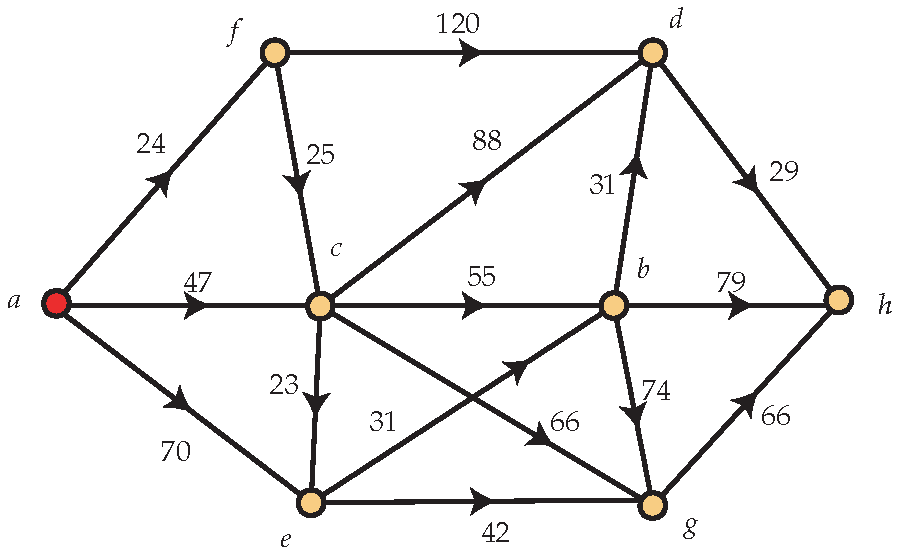
\includegraphics[width=\linewidth]{images/dijkstragraph}
\end{image}%
\tcblower
\end{figureptx}%
Suppose that the root vertex \(r\) is the vertex labeled~\(a\). The initialization step of Dijkstra's algorithm then results in the following values for \(\delta\) and \(P\):%
\begin{paragraphs}{Step 1. Initialization.}{g:paragraphs:idp128}%
%
\begin{align*}
\sigma\amp=(a)\amp\amp\\
\delta(a)\amp=0; \amp P(a)\amp=(a)\\
\delta(b) \amp=\infty; \amp P(b)\amp=(a,b)\\
\delta(c) \amp=47; \amp P(c)\amp=(a,c)\\
\delta(d) \amp=\infty; \amp P(d)\amp=(a,d)\\
\delta(e) \amp=70; \amp P(e)\amp=(a,e)\\
\delta(f) \amp=24; \amp P(f)\amp=(a,f)\\
\delta(g) \amp=\infty; \amp P(g)\amp=(a,g)\\
\delta(h) \amp=\infty; \amp P(h)\amp=(a,h)
\end{align*}
%
\par
Before finishing Step 1, the algorithm identifies vertex~\(f\) as closest to \(a\) and appends it to \(\sigma\), making \(a\) permanent. When entering Step 2, Dijkstra's algorithm attempts to find shorter paths from \(a\) to each of the temporary vertices by going through \(f\). We call this process ``scanning from vertex~\(f\).'' In this scan, the path to vertex~\(d\) is updated, since \(\delta(f) + w(f,d)=24+120=144\lt \infty=w(a,d)\).%
\end{paragraphs}%
\begin{paragraphs}{Step 2.  Scan from vertex~\(f\).}{g:paragraphs:idp129}%
%
\begin{align*}
\sigma\amp=(a,f)\amp\amp\\
\delta(a)\amp=0; \amp P(a)\amp=(a)\\
\delta(b)\amp=\infty; \amp P(b)\amp=(a,b)\\
\delta(c)\amp=47; \amp P(c)\amp=(a,c)\\
\delta(d)\amp=144 = 24 + 120 = \delta(f)+w(f,d); \amp P(d)\amp=(a,f,d)\quad\text{updated} \\
\delta(e)\amp=70; \amp P(e)\amp=(a,e)\\
\delta(f)\amp=24; \amp P(f)\amp=(a,f)\\
\delta(g)\amp=\infty; \amp P(g)\amp=(a,f)\\
\delta(h)\amp=\infty; \amp P(h)\amp=(a,h)
\end{align*}
%
\par
Before proceeding to the next step, vertex~\(c\) is made permanent by making it \(v_3\). In Step 3, therefore, the scan is from vertex \(c\). Vertices \(b\), \(d\), and \(g\) have their paths updated. However, although \(\delta(c) + w(c,e) = 47+23=70=\delta(e)\), we do not change \(P(e)\) since \(\delta(e)\) is not \emph{decreased} by routing \(P(e)\) through \(c\).%
\end{paragraphs}%
\begin{paragraphs}{Step 3.  Scan from vertex~\(c\).}{g:paragraphs:idp130}%
%
\begin{align*}
\sigma\amp=(a,f,c)\\
\delta(a)\amp=0; \amp P(a)\amp=(a)\\
\delta(b)\amp=102=47+55= \delta(c)+w(c,b); \amp P(b)\amp=(a,c,b)\quad\text{updated}\\
\delta(c)\amp=47; \amp P(c)\amp=(a,c)\\
\delta(d)\amp=135=47+88 = \delta(c)+w(c,d); \amp P(d)\amp=(a,c,d)\quad\text{updated} \\
\delta(e)\amp=70; \amp P(e)\amp=(a,e)\\
\delta(f)\amp=24; \amp P(f)\amp=(a,f)\\
\delta(g)\amp=113=47+66= \delta(c)+w(c,g); \amp P(g)\amp=(a,c,g)\quad\text{updated} \\
\delta(h)\amp=\infty; \amp P(h)\amp=(a,h)
\end{align*}
%
\par
Now vertex \(e\) is made permanent.%
\end{paragraphs}%
\begin{paragraphs}{Step 4.  Scan from vertex~\(e\).}{g:paragraphs:idp131}%
%
\begin{align*}
\sigma\amp=(a,f,c,e)\\
\delta(a)\amp=0; \amp P(a)\amp=(a)\\
\delta(b)\amp=101=70+31= \delta(e)+w(e,b); \amp P(b)\amp=(a,e,b)\quad\text{updated}\\
\delta(c)\amp=47; \amp P(c)\amp=(a,c)\\
\delta(d)\amp=135; \amp P(d)\amp=(a,c,d)\\
\delta(e)\amp=70; \amp P(e)\amp=(a,e)\\
\delta(f)\amp=24; \amp P(f)\amp=(a,f)\\
\delta(g)\amp=112=70+42= \delta(e)+w(e,g); \amp P(g)\amp=(a,e,g)\quad\text{updated}\\
\delta(h)\amp=\infty; \amp P(h)\amp=(a,h)
\end{align*}
%
\par
Now vertex \(b\) is made permanent.%
\end{paragraphs}%
\begin{paragraphs}{Step 5.  Scan from vertex~\(b\).}{g:paragraphs:idp132}%
%
\begin{align*}
\sigma\amp=(a,f,c,e,b)\\
\delta(a)\amp=0; \amp P(a)\amp=(a)\\
\delta(b)\amp=101; \amp P(b)\amp=(a,e,b)\\
\delta(c)\amp=47; \amp P(c)\amp=(a,c)\\
\delta(d)\amp= 132 = 101+ 31= \delta(b)+w(b,d); \amp P(d)\amp=(a,e,b,d)\quad\text{updated} \\
\delta(e)\amp= 70; \amp P(e)\amp=(a,e)\\
\delta(f)\amp= 24; \amp P(f)\amp=(a,f)\\
\delta(g)\amp=112; \amp P(g)\amp=(a,e,g)\\
\delta(h)\amp=180 = 101+79=\delta(b)+w(b,h); \amp P(h)\amp=(a,e,b,h)\quad\text{updated} 
\end{align*}
%
\par
Now vertex \(g\) is made permanent.%
\end{paragraphs}%
\begin{paragraphs}{Step 6.  Scan from vertex~\(g\).}{g:paragraphs:idp133}%
%
\begin{align*}
\sigma\amp=(a,f,c,e,b,g)\\
\delta(a)\amp=0; \amp P(a)\amp=(a)\\
\delta(b)\amp=101; \amp P(b)\amp=(a,e,b)\\
\delta(c)\amp=47; \amp P(c)\amp=(a,c)\\
\delta(d)\amp= 132; \amp P(d)\amp=(a,e,b,d)\\
\delta(e)\amp=70; \amp P(e)\amp=(a,e)\\
\delta(f)\amp=24; \amp P(f)\amp=(a,f)\\
\delta(g)\amp=112; \amp P(g)\amp=(a,e,g)\\
\delta(h)\amp=178 = 112+66=\delta(g)+w(g,h); \amp P(h)\amp=(a,e,g,h)\quad\text{updated}
\end{align*}
%
\par
Now vertex \(d\) is made permanent.%
\end{paragraphs}%
\begin{paragraphs}{Step 7.  Scan from vertex~\(d\).}{g:paragraphs:idp134}%
%
\begin{align*}
\sigma\amp=(a,f,c,e,b,g,d)\\
\delta(a)\amp=0; \amp P(a)\amp=(a)\\
\delta(b)\amp=101; \amp P(b)\amp=(a,e,b)\\
\delta(c)\amp=47; \amp P(c)\amp=(a,c)\\
\delta(d)\amp= 132; \amp P(d)\amp=(a,e,b,d)\\
\delta(e)\amp=70; \amp P(e)\amp=(a,e)\\
\delta(f)\amp=24; \amp P(f)\amp=(a,f)\\
\delta(g)\amp=112; \amp P(g)\amp=(a,e,g)\\
\delta(h)\amp=161 = 132+29=\delta(d)+w(d,h); \amp P(h)\amp=(a,e,b,d,h)\quad\text{updated}
\end{align*}
%
\par
Now vertex \(h\) is made permanent. Since this is the last vertex, the algorithm halts and returns the following:%
\end{paragraphs}%
\begin{paragraphs}{Final Results of Dijkstra's Algorithm.}{g:paragraphs:idp135}%
%
\begin{align*}
\sigma\amp=(a,f,c,e,b,g,d,h)\\
\delta(a)\amp=0; \amp P(a)\amp=(a)\\
\delta(b)\amp=101; \amp P(b)\amp=(a,e,b)\\
\delta(c)\amp=47; \amp P(c)\amp=(a,c)\\
\delta(d)\amp= 132; \amp P(d)\amp=(a,e,b,d)\\
\delta(e)\amp=70; \amp P(e)\amp=(a,e)\\
\delta(f)\amp=24; \amp P(f)\amp=(a,f)\\
\delta(g)\amp=112; \amp P(g)\amp=(a,e,g)\\
\delta(h)\amp=161; \amp P(h)\amp=(a,e,b,d,h)
\end{align*}
%
\end{paragraphs}%
\end{subsectionptx}
%
%
\typeout{************************************************}
\typeout{Subsection 3.4.3 The Correctness of Dijkstra's Algorithm}
\typeout{************************************************}
%
\begin{subsectionptx}{The Correctness of Dijkstra's Algorithm}{}{The Correctness of Dijkstra's Algorithm}{}{}{g:subsection:idp136}
Now that we've illustrated Dijkstra's algorithm, it's time to prove that it actually does what we claimed it does: find the distance from the root vertex to each of the other vertices and a path of that length. To do this, we first state two elementary propositions. The first is about shortest paths in general, while the second is specific to the sequence of permanent vertices produced by Dijkstra's algorithm.%
\begin{proposition}{}{}{g:proposition:idp137}%
Let \(x\) be a vertex and let \(P=(r=u_0,u_1,\dots,u_t=x)\) be a shortest path from \(r\) to \(x\). Then for every integer \(j\) with \(0\lt j\lt t\), \((u_0,u_1,\dots,u_j)\) is a shortest path from \(r\) to \(u_j\) and \((u_j,u_{j+1},\dots,u_t)\) is a shortest path from \(u_j\) to \(u_t\)%
\end{proposition}
\begin{proposition}{}{}{g:proposition:idp138}%
When the algorithm halts, let \(\sigma=(v_1,v_2,v_3,\dots,v_n)\).  Then%
\begin{equation*}
\delta(v_1)\le \delta(v_2)\le\dots \le \delta(v_n).
\end{equation*}
%
\end{proposition}
We are now ready to prove the correctness of the algorithm. The proof we give will be inductive, but the induction will have nothing to do with the total number of vertices in the digraph or the step number the algorithm is in.%
\begin{theorem}{}{}{g:theorem:idp139}%
Dijkstra's algorithm yields shortest paths for every vertex \(x\) in \(\bfG\). That is, when Dijkstra's algorithm terminates, for each \(x\in V\), the value \(\delta(x)\) is the distance from \(r\) to \(x\) and \(P(x)\) is a shortest path from \(r\) to \(x\).%
\end{theorem}
\begin{proof}{}{g:proof:idp140}
The theorem holds trivially when \(x=r\). So we consider the case where \(x\neq r\). We argue that \(\delta(x)\) is the distance from \(r\) to \(x\) and that \(P(x)\) is a shortest path from \(r\) to \(x\) by induction on the minimum number \(k\) of edges in a shortest path from \(r\) to \(x\). When \(k=1\), the edge \((r,x)\) is a shortest path from \(r\) to \(x\). Since \(v_1=r\), we will set \(\delta(x)=w(r,x)\) and \(P(x)=(r,x)\) at Step~1.%
\par
Now fix a positive integer \(k\). Assume that if the minimum number of edges in a shortest path from \(r\) to \(x\) is at most \(k\), then \(\delta(x)\) is the distance from \(r\) to \(x\) and \(P(x)\) is a shortest path from \(r\) to \(x\). Let \(x\) be a vertex for which the minimum number of edges in a shortest path from \(r\) to \(x\) is \(k+1\). Fix a shortest path \(P=(u_0,u_1,u_2,\dots,u_{k+1})\) from \(r=u_0\) to \(x=u_{k+1}\). Then \(Q=(u_0,u_1,\dots,u_k)\) is a shortest path from \(r\) to \(u_k\). (See \hyperref[x:figure:fig_graphalgorithms_dijkstra-proof]{Figure~{\xreffont\ref{x:figure:fig_graphalgorithms_dijkstra-proof}}}.)%
\begin{figureptx}{Shortest paths}{x:figure:fig_graphalgorithms_dijkstra-proof}{}%
\begin{image}{0.125}{0.75}{0.125}%
\resizebox{\linewidth}{!}{%
\begin{overpic}[width=0.6\textwidth]{images/dijkstra-proof}
                        \put(3,13){\(r\)}
                        \put(33,25){\(Q\)}
                        \put(58,3){\(P(u_k)\)}
                        \put(73,28){\(u_k\)}
                        \put(83,25){\(P\)}
                        \put(93,21){\(x\)}
                        \end{overpic}
}%
\end{image}%
\tcblower
\end{figureptx}%
By the inductive hypothesis, \(\delta(u_k)\) is the distance from \(r\) to \(u_k\), and \(P(u_k)\) is a shortest path from \(r\) to \(u_k\). Note that \(P(u_k)\) need not be the same as path \(Q\), as we suggest in \hyperref[x:figure:fig_graphalgorithms_dijkstra-proof]{Figure~{\xreffont\ref{x:figure:fig_graphalgorithms_dijkstra-proof}}}. However, if distinct, the two paths will have the same length, namely \(\delta(u_k)\).  Also, the distance from \(r\) to \(x\) is \(\delta(u_k)+w(u_k,x)\ge \delta(u_k)\) since \(P\) is a shortest path from \(r\) to \(x\) and \(w(u_k,x)\geq 0\).%
\par
Let \(i\) and \(j\) be the unique integers for which \(u_k=v_i\) and \(x=v_j\). If \(j \lt i\), then%
\begin{equation*}
\delta(x)= \delta(v_j)\le \delta(v_i)= \delta(u_k)\le
\delta(u_k)+w(u_k).
\end{equation*}
Therefore the algorithm has found a path \(P(x)\) from \(r\) to \(x\) having length \(\delta(x)\) which is at most the distance from \(r\) to \(x\). Clearly, this implies that \(\delta(x)\) is the distance from \(r\) to \(x\) and that \(P(x)\) is a shortest path.%
\par
On the other hand, if \(j>i\), then the inductive step at Step~\(i\) results in%
\begin{equation*}
\delta(x)\le \delta(v_i)+w(v_i,y)=\delta(u_k)+w(u_k,x).
\end{equation*}
As before, this implies that \(\delta(x)\) is the distance from \(r\) to \(x\) and that \(P(x)\) is a shortest path.%
\end{proof}
\end{subsectionptx}
\end{sectionptx}
%
%
\typeout{************************************************}
\typeout{Section 3.5 Algorithm for Longest Paths}
\typeout{************************************************}
%
\begin{sectionptx}{Algorithm for Longest Paths}{}{Algorithm for Longest Paths}{}{}{x:section:s_graphalgorithms_longest-paths}
\begin{introduction}{}%
To complement Dijkstra's algorithm for finding the short path, in this section we give an algorithm for finding the \emph{longest} path between two vertices in a directed graph.%
\par
It is not immediately clear why we might want to do this, so first in \hyperref[x:subsection:subs_graphalgorithms_longest-path-motivation]{Subsection~{\xreffont\ref{x:subsection:subs_graphalgorithms_longest-path-motivation}}}   we give a motivational problem: scheduling work on a complicated project.  The algorithm we present will only work on \emph{acyclic} directed graphs, so in \hyperref[x:subsection:subs_graphalgorithms_longest-path-acyclic-sort]{Subsection~{\xreffont\ref{x:subsection:subs_graphalgorithms_longest-path-acyclic-sort}}} we define these, explain why this isn't a restriction for our intended application, and give the first step of the algorithm: "topologically sorting" the vertices of an acyclic directed graph.  Finally, in \hyperref[x:subsection:subs_graphalgorithms_longest-path-algorithm]{Subsection~{\xreffont\ref{x:subsection:subs_graphalgorithms_longest-path-algorithm}}}   we explain the actual algorithm.%
\end{introduction}%
%
%
\typeout{************************************************}
\typeout{Subsection 3.5.1 }
\typeout{************************************************}
%
\begin{subsectionptx}{}{}{}{}{}{x:subsection:subs_graphalgorithms_longest-path-motivation}
The main application of the longest path algorithm is in scheduling.  Suppose we have a large project -{}-{} say, building a house -{}-{} that is composed of many smaller projects: digging the foundation, building the walls, connecting to gas, electricity, and water, building the roof, doing the interiors, landscaping, etc.%
\par
Some of these activities will require others to be done before them (you can't put the roof on before you've built the walls; you don't want to do the landscaping before you've dug your water lines), while others could be done at the same time (finishing the interiors and doing the landscaping).  Each sub-job has an expected amount of time required to finish it; you'd like to know before hand how long the whole task will take, and when the various sub-jobs should be done so you can arrange the contractors.%
\par
From a series of jobs like this, we will construct a weighted, directed, acyclic graph.  The edges will be the sub-jobs. The weights of each edge will be the expected length of time that job has.  The structure of the graph will encode the dependencies of the subjobs on each other -{}-{} an edge \(e\) will flow into an edge \(f\) if the job \(f\) immediately depends about the job \(e\).%
\par
We will work out the construction of this graph in one example.  It is not always trivial to construct the directed graph from the table of jobs and dependencies.  It is not clear what the vertices should be, and sometimes dummy edges and vertices need to be encoded.  You do not need to worry about constructing these graphs in general, though if you're curious it can be interesting to think about.  Any exam question about this topic would supply you with the directed graph.%
 Example === Consider the following table, listing tasks \textdollar{}\textdollar{}A-H\textdollar{}\textdollar{}, the expected time of completion for each task, and the required tasks before a given task can be started. \begin{tableptx}{\textbf{}}{g:table:idp141}{}%
Task Time PrerequisitesA 6 B 7 C 4 AD 3 AE 4 B,DF 10 CG 3 CH 10 E,G\end{tableptx}%
 Here is the corresponding graph encoding this information: \begin{image}{0}{1}{0}%
\end{image}%
 Construction of the graph ==== We outline how the graph above was constructed.  We make one vertex for the start, one vertex for the finish, and then another vertex for each set of dependencies, that is, the entries in the third column.  Then we draw an edge for each letter, beginning at the vertex corresponding to its set of prerequisites (or the start, if it has none), and ending at the vertex that contains it as a prerequisite (or the end, if no tasks require it as a prerequisite). Note that this method works only if any two sets of prerequisites either have nontrivial intersection or are identical.  The tricky cases you don't have to worry about are when this isn't true. Longest Paths -{}-{}-{}-{} With that detour out of the way, we see why finding the longest path in a directed acyclic graph is useful: in case the edges are tasks and the weights are expected times, the length of the longest path is the minimal time the whole project would be able to be completed. Moreover, it is useful to actually know what the longest paths are -{}-{} to achieve this minimal time, each task in the longest path must be completed in the expected amount of time, and the next task in the path must be started immediately when the first one finishes.  For this reason, the longest paths are known as \textasteriskcentered{}critical paths\textasteriskcentered{}.\end{subsectionptx}
%
%
\typeout{************************************************}
\typeout{Subsection 3.5.2 }
\typeout{************************************************}
%
\begin{subsectionptx}{}{}{}{}{}{x:subsection:subs_graphalgorithms_longest-path-acyclic-sort}
\end{subsectionptx}
%
%
\typeout{************************************************}
\typeout{Subsection 3.5.3 }
\typeout{************************************************}
%
\begin{subsectionptx}{}{}{}{}{}{x:subsection:subs_graphalgorithms_longest-path-algorithm}
\end{subsectionptx}
\end{sectionptx}
%
%
\typeout{************************************************}
\typeout{Section 3.6 The Traveling Salesperson Problem}
\typeout{************************************************}
%
\begin{sectionptx}{The Traveling Salesperson Problem}{}{The Traveling Salesperson Problem}{}{}{x:section:s_graphalgorithms_traveling-salesperson}
\begin{introduction}{}%
In this section we discuss the Travelling Salesperson problem.  In \hyperref[x:subsection:subs_graphalgorithms_tsp_intro]{Subsection~{\xreffont\ref{x:subsection:subs_graphalgorithms_tsp_intro}}}  we introduce the problem and give some explanation of why it is very hard in general.  Rather than try to solve it exactly, we will resort to providing upper and lower bounds for the solution.  In \hyperref[x:subsection:subs_graphalgorithms_tsp_upper]{Subsection~{\xreffont\ref{x:subsection:subs_graphalgorithms_tsp_upper}}}  we discuss various methods of constructing upper bounds.  In \hyperref[x:subsection:subs_graphalgorithms_tsp_lower]{Subsection~{\xreffont\ref{x:subsection:subs_graphalgorithms_tsp_lower}}}  we give a method of constructing lower bounds.%
\end{introduction}%
%
%
\typeout{************************************************}
\typeout{Subsection 3.6.1 Introduction to the Traveling Salesperson Problem}
\typeout{************************************************}
%
\begin{subsectionptx}{Introduction to the Traveling Salesperson Problem}{}{Introduction to the Traveling Salesperson Problem}{}{}{x:subsection:subs_graphalgorithms_tsp_intro}
Let us first describe the Traveling Salesperson Problem, or TSP for short, in informal language, and then translate it into a question about graph theory.%
\par
Imagine you work for a company, travelling from city to city, trying to sell some product in each (for instance, encyclopedias).  You are assigned a list of cities you need to visit, and you need to start from your home, travel from city to city visiting them all, and finally return to your home.  Of course, travelling from city to city is expensive (either in terms of money, travel time, or something else), and to turn a profit your company wants you to organize the order you visit each of cities so that the total cost is as cheap as possible.  This minimiziation problem is the TSP.%
\par
Translated into graph theory, the TSP can be succinctly stated as follows: given a weighted graph \(\bfG\), find the cheapest Hamiltonian path. That is, the cheapest closed walk on \(\bfG\) that visits every vertex exactly once.%
\par
First, note that it is enough to consider the complete graph \(K_n\).  If we are given some other weighted graph \(\bfG\), we can add all the edges not in \(\bfG\) but make their weights \emph{much} larger than any of the weights inside \(\bfG\).%
\par
Another important point is that the problem of determining whether a given graph \(\bfG\) has a Hamiltonian cycle is a special case of the traveling salesman problem.  To see this, suppose we're given a graph \(\bfG\), and we want to determine whether it is Hamiltonian.  We create a weighted \(K_n\), with vertices the vertices of \(\bfG\) by giving the edge \(v-w\) a very small weight \(\epsilon\) if \(v\) and \(w\) \emph{are} adjacent in \(\bfG\), and a very large weight \(M\) if \(v\) and \(w\) \textasteriskcentered{}are not\textasteriskcentered{} adjacent in \(\bfG\).  Then, any Hamiltonian path in \(\bfG\) would have cost \(n\epsilon\), where as any path that uses an edge not in \(\bfG\) costs more than \(M\).  So, if we make \(M>n\epsilon\), the TSP for our weighted \(K_n\) will have a solution with cost less than \(M\) if and only if \(\bfG\) had a Hamiltonian cycle.%
\par
Since determining whether a graph \(\bfG\) is Hamiltonian is difficult (NP complete), the TSP will also be.  As such, we will not discuss any algorithms for actually solving TSP.  Instead, we will discuss methods for giving upper and lower bounds for the TSP.%
\end{subsectionptx}
%
%
\typeout{************************************************}
\typeout{Subsection 3.6.2 Finding upper bounds to the TSP}
\typeout{************************************************}
%
\begin{subsectionptx}{Finding upper bounds to the TSP}{}{Finding upper bounds to the TSP}{}{}{x:subsection:subs_graphalgorithms_tsp_upper}
Getting \emph{good} upper bounds to the TSP will turns out to be difficult.  However, finding not so good upper bounds will turn out to be quite easy.%
\par
For instance, any solution to the TSP will be a Hamiltonian cycle, and in particular if \(\bfG\) contains \(n\) vertices, the TSP solution will contain \(n\) edges.  Let \(M\) be the weight of the most expensive edge in \(\bfG\).%
%
\begin{equation*}
w(C)=\sum_{i=1}^n w(e_i)\leq \sum_{i=1}^ M = nM
\end{equation*}
Since the TSP asks for the cheapeast Hamiltonian cycle, taking \emph{any} Hamiltonian cycle and calculating its cost will be an upper bound for the TSP.  Just choosing a random Hamiltonian cycle will in general be very expensive and silly -{}-{} for instance, going from Sheffield to London to Rotherham to Edinburgh to Chesterfield to Glasgow to Nottingham to Brighton is clearly not optimal.%
\par
A greedy algorithm will give a heuristically better result: we call it the \emph{nearst neighbor algorithm}.  At each step, simply go to the nearest city you have not already visited.  This will give good results at the beginning, but since we do not do any planning ahead, it will in general give bad results, as the following example illustrates:%
\begin{figureptx}{The graph \(\bfG\) where nearest neighbour struggles}{x:figure:fig_nearestneighbourbadexample}{}%
\begin{image}{0.15}{0.7}{0.15}%
\resizebox{\linewidth}{!}{%
\begin{tikzpicture} 
\begin{scope}[xscale=2,  every node/.style={circle, thick, draw}]
\foreach \x in {0,1,...,9} \node (\x) at (-108-36*\x:3) {$v_\x$};
      \node (w) at (0,7) {$w$};
      \draw (0)--(1)--(2)--(3)--(4)--(5)--(6)--(7)--(8)--(9)--(w)--(0);
\end{scope}
\end{tikzpicture}
}%
\end{image}%
\tcblower
\end{figureptx}%
Consider running the Nearest Neighbor algorithm starting at \(v_0\).  At the first step, we have a choice -{}-{} we could go to \(v_1\) or to \(v_9\).  Suppose we go to \(v_1\).  After that, our choice is forced -{}-{} \(v_1-v_2-v_3-v_4-v_5-v_6-v_7-v_8-v_9\) costs one at each step.  Now, we still have to visit \(T\) before returning to \(V_0\), which will cost us 10 to detour through.  We clearly should have planned ahead and visited \textdollar{}\textdollar{}T\textdollar{}\textdollar{} in between vertices \(v_4\) and \(v_5\) at a cost of 4.%
\par
Clearly the nearest neighbour algorithm is not in general very good, and better algorithms are possible.  We present it first to give a quick but reasonable way to get a solution to TSP that isn't \emph{completely} horrible, and second to illustrate that greedy algorithms in general will not be efficient.  We briefly mention two other ways to get lower bounds.%
\par
Another, slightly better, greedy algorithm might be called \emph{nearest insertion}.  It inductively builds bigger and bigger closed loops one vertex at time.  When there is a closed loop with \emph{k} vertices \(v_1-v_2-v_3-\cdots - v_k-v_1\) and we want to add vertex \(w\) to the loop, we look at each of the adjacent legs \(v_i-v_{i+1}\), and determine how much it would raise the cost to insert the next vertex \(w\) in between those two cities (changing the path to \(v_1-w-v_{i+1}\)), being sure to also check for inserting it between \(v_k\) and \(v_1\).  This does much better at our example above, but can run into other problems, and involves a little more bookkeeping and arithmetic, so I won't ask you to implement it on the exam.%
\par
Another method inolves a qualitive change of view.  The greedy algorithms we describe so far are only heuristics to getting a decent path.  There is no guarantee that they produce an output that is in any way close to the optimal path, and indeed examples can be engineered to make them extremely bad.  It would be nice to have an upper bound that was guaranteed to not be \emph{too} far off the optimal solution.  The Christofides algorithm does just that, by producing a Hamiltonian cycle that is guaranteed to have weight at most 3\slash{}2 of the weight of the optimal solution.  Very briefly, it does this by starting with a minimal weight spanning tree, makes a subgraph by adding edges to the tree until every vertex has even degree, taking an Eulerian circuit of that, and then removing edges to get a Hamiltonian cycle.%
\par
For nearly fifty years, Christofides algorithm was the best known guaranteed upper bound on the Travelling Salesperson problem, but in the summer 2020 of Nathan Klein, Anna Karlin and Shayan Oveis Gharan managed to modify the algorithm to give a very slight improvement, producing a cycle guaranteed to be within \(3/2-\varepsilon\) for some \(\varepsilon>10^{-36}\).  See this Quanta article for a popular account of their work.%
\end{subsectionptx}
%
%
\typeout{************************************************}
\typeout{Subsection 3.6.3 A lower point for TSP}
\typeout{************************************************}
%
\begin{subsectionptx}{A lower point for TSP}{}{A lower point for TSP}{}{}{x:subsection:subs_graphalgorithms_tsp_lower}
To get a lower bound for TSP we have to be a little more intelligent.  Suppose we had a solution \(C\) to the TSP for \(\Gamma\), and that we deleted one vertex \(v\) from \(C\).  Deleting a vertex from a cycle gives us a path \(P\), and in particular a tree.  Furthermore, \(P\) visits every vertex in \(\Gamma\) except for \(v\), and so it is a spanning tree of \(\Gamma\setminus v\).%
\par
We can use Kruskal's algorithm (or another) to find a minimal spanning tree \(T\) of \(\Gamma\setminus v\), and we have that \(w(P)\geq w(T)\).  The cycle \(C\) contains just two more edges, from \(v\) to two other vertices, say \(a\) and \(b\).  We can obtain lower bounds on the weights of the edges \(v-a\) and \(v-b\) by taking the weights of the lowest two edges out of \(v\), maybe \(e_1\) and \(e_2\).  We have%
%
\begin{equation*}
w(C)=w(P)+w(a-v)+w(b-v)\geq w(T)+w(e_1)+w(e_2)
\end{equation*}
giving us a lower bound on solutions to the TSP.%
\end{subsectionptx}
\end{sectionptx}
%
%
\typeout{************************************************}
\typeout{Exercises 3.7 Exercises}
\typeout{************************************************}
%
\begin{exercises-section}{Exercises}{}{Exercises}{}{}{x:exercises:s_graphalgorithms_exercises}
\begin{divisionexercise}{1}{}{}{g:exercise:idp142}%
For the graph in \hyperref[x:figure:fig_span_tree_ex1]{Figure~{\xreffont\ref{x:figure:fig_span_tree_ex1}}}, use Kruskal's algorithm (``avoid cycles'') to find a minimum weight spanning tree. Your answer should include a complete list of the edges, indicating which edges you take for your tree and which (if any) you reject in the course of running the algorithm.%
\begin{figureptx}{Find a minimum weight spanning tree}{x:figure:fig_span_tree_ex1}{}%
\begin{image}{0.175}{0.65}{0.175}%
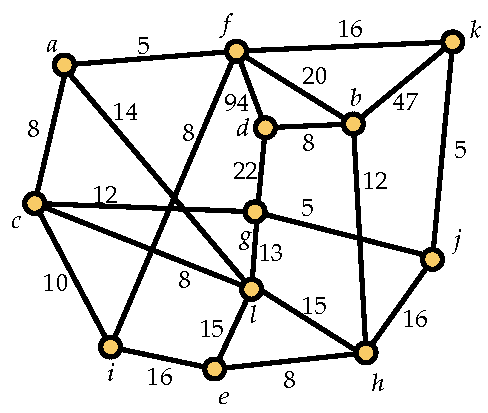
\includegraphics[width=\linewidth]{images/span_tree_ex1}
\end{image}%
\tcblower
\end{figureptx}%
\end{divisionexercise}%
\begin{divisionexercise}{2}{}{}{g:exercise:idp143}%
For the graph in \hyperref[x:figure:fig_span_tree_ex1]{Figure~{\xreffont\ref{x:figure:fig_span_tree_ex1}}}, use Prim's algorithm (``build tree'') to find a minimum weight spanning tree. Your answer should list the edges selected by the algorithm in the order they were selected.%
\end{divisionexercise}%
\begin{divisionexercise}{3}{}{}{g:exercise:idp144}%
For the graph in \hyperref[x:figure:fig_span_tree_ex2]{Figure~{\xreffont\ref{x:figure:fig_span_tree_ex2}}}, use Kruskal's algorithm (``avoid cycles'') to find a minimum weight spanning tree. Your answer should include a complete list of the edges, indicating which edges you take for your tree and which (if any) you reject in the course of running the algorithm.%
\begin{figureptx}{Find a minimum weight spanning tree}{x:figure:fig_span_tree_ex2}{}%
\begin{image}{0.175}{0.65}{0.175}%
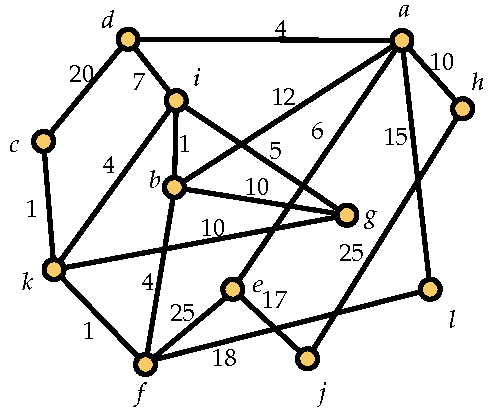
\includegraphics[width=\linewidth]{images/span_tree_ex2}
\end{image}%
\tcblower
\end{figureptx}%
\end{divisionexercise}%
\begin{divisionexercise}{4}{}{}{g:exercise:idp145}%
For the graph in \hyperref[x:figure:fig_span_tree_ex2]{Figure~{\xreffont\ref{x:figure:fig_span_tree_ex2}}}, use Prim's algorithm (``build tree'') to find a minimum weight spanning tree. Your answer should list the edges selected by the algorithm in the order they were selected.%
\end{divisionexercise}%
\begin{divisionexercise}{5}{}{}{g:exercise:idp146}%
For the graph in \hyperref[x:figure:fig_span_tree_ex3]{Figure~{\xreffont\ref{x:figure:fig_span_tree_ex3}}}, use Kruskal's algorithm (``avoid cycles'') to find a minimum weight spanning tree. Your answer should include a complete list of the edges, indicating which edges you take for your tree and which (if any) you reject in the course of running the algorithm.%
\begin{figureptx}{Find a minimum weight spanning tree}{x:figure:fig_span_tree_ex3}{}%
\begin{image}{0.275}{0.45}{0.275}%
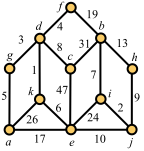
\includegraphics[width=\linewidth]{images/span_tree_ex3}
\end{image}%
\tcblower
\end{figureptx}%
\end{divisionexercise}%
\begin{divisionexercise}{6}{}{}{g:exercise:idp147}%
For the graph in \hyperref[x:figure:fig_span_tree_ex3]{Figure~{\xreffont\ref{x:figure:fig_span_tree_ex3}}}, use Prim's algorithm (``build tree'') to find a minimum weight spanning tree. Your answer should list the edges selected by the algorithm in the order they were selected.%
\end{divisionexercise}%
\begin{divisionexercise}{7}{}{}{g:exercise:idp148}%
A new local bank is being created and will establish a headquarters \(h\), two branches \(b_1\) and \(b_2\), and four ATMs \(a_1\), \(a_2\), \(a_3\), and \(a_4\). They need to build a computer network such that the headquarters, branches, and ATMs can all intercommunicate. Furthermore, they will need to be networked with the Federal Reserve Bank of Atlanta, \(f\). The costs of the feasible network connections (in units of \textdollar{}10,000) are listed below:%
\begin{align*}
h f \amp  \quad 80 \amp 
h b_1 \amp  \quad 10\amp  h b_2 \amp  \quad 20\amp 
b_1 b_2 \amp  \quad 8\\
f b_1 \amp  \quad 12\amp 
f a_1 \amp  \quad 20\amp  b_1 a_1 \amp  \quad 3\amp 
a_1 a_2 \amp  \quad 13\\
h a_2 \amp  \quad 6\amp 
b_2 a_2 \amp  \quad 9\amp  b_2 a_3 \amp  \quad 40\amp 
a_1 a_4 \amp  \quad 3\\
a_3 a_4 \amp \quad 6
\end{align*}
The bank wishes to minimize the cost of building its network (which must allow for connection, possibly routed through other nodes, from each node to each other node), however due to the need for high-speed communication, they \alert{must} pay to build the connection from \(h\) to \(f\) as well as the connection from \(b_2\) to \(a_3\). Give a list of the connections the bank should establish in order to minimize their total cost, subject to this constraint. Be sure to explain how you selected the connections and how you know the total cost is minimized.%
\end{divisionexercise}%
\begin{divisionexercise}{8}{}{}{g:exercise:idp149}%
A disconnected weighted graph obviously has no spanning trees. However, it is possible to find a spanning forest of minimum weight in such a graph. Explain how to modify both Kruskal's algorithm and Prim's algorithm to do this.%
\end{divisionexercise}%
\begin{divisionexercise}{9}{}{}{g:exercise:idp150}%
Prove \hyperref[x:proposition:prop_graphalgorithms_spanforest]{Proposition~{\xreffont\ref{x:proposition:prop_graphalgorithms_spanforest}}}.%
\end{divisionexercise}%
\begin{divisionexercise}{10}{}{}{g:exercise:idp151}%
In the paper where Kruskal's algorithm first appeared, he considered the algorithm a route to a nicer proof that in a connected weighted graph with no two edges having the same weight, there is a \emph{unique} minimum weight spanning tree. Prove this fact using Kruskal's algorithm.%
\end{divisionexercise}%
\begin{divisionexercise}{11}{}{}{g:exercise:idp152}%
Use Dijkstra's algorithm to find the distance from \(a\) to each other vertex in the digraph shown in \hyperref[x:figure:fig_graphalgorithms_dijkstra_ex1]{Figure~{\xreffont\ref{x:figure:fig_graphalgorithms_dijkstra_ex1}}} and a directed path of that length.%
\begin{figureptx}{A directed graph}{x:figure:fig_graphalgorithms_dijkstra_ex1}{}%
\begin{image}{0.175}{0.65}{0.175}%
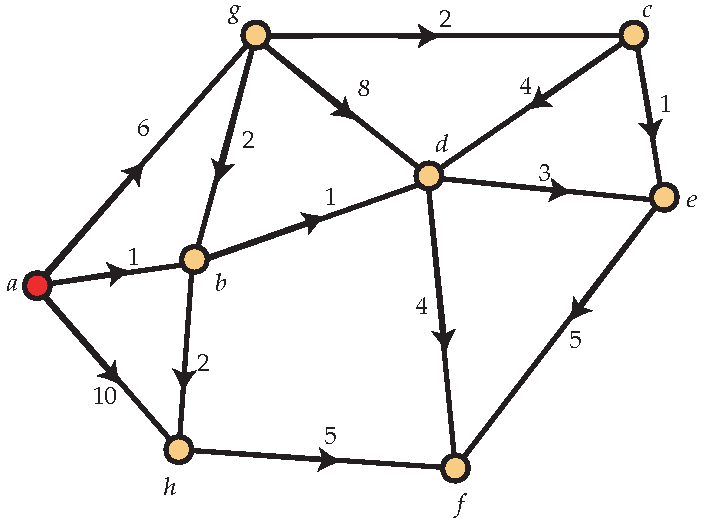
\includegraphics[width=\linewidth]{images/dijkstra_ex1}
\end{image}%
\tcblower
\end{figureptx}%
\end{divisionexercise}%
\begin{divisionexercise}{12}{}{}{g:exercise:idp153}%
\hyperref[x:table:tab_digraph1]{Table~{\xreffont\ref{x:table:tab_digraph1}}} contains the length of the directed edge \((x,y)\) in the intersection of \emph{row} \(x\) and \emph{column} \(y\) in a digraph with vertex set \(\{a,b,c,d,e,f\}\). For example, \(w(b,d)=21\). (On the other hand, \(w(d,b)=10\).) Use this data and Dijkstra's algorithm to find the distance from \(a\) to each of the other vertices and a directed path of that length from \(a\).%
\begin{tableptx}{\textbf{A digraph represented as a table of data}}{x:table:tab_digraph1}{}%
\centering%
{\tabularfont%
\begin{tabular}{lAllllll}
\(w\)&\(a\)&\(b\)&\(c\)&\(d\)&\(e\)&\(f\)\tabularnewline\hrulethin
\(a\)&0&12&8&43&79&35\tabularnewline[0pt]
\(b\)&93&0&18&21&60&33\tabularnewline[0pt]
\(c\)&17&3&0&37&50&30\tabularnewline[0pt]
\(d\)&85&10&91&0&17&7\tabularnewline[0pt]
\(e\)&28&47&39&14&0&108\tabularnewline[0pt]
\(f\)&31&7&29&73&20&0
\end{tabular}
}%
\end{tableptx}%
\end{divisionexercise}%
\begin{divisionexercise}{13}{}{}{g:exercise:idp154}%
Use Dijkstra's algorithm to find the distance from \(a\) to each other vertex in the digraph shown in \hyperref[x:figure:fig_graphalgorithms_dijkstra_ex2]{Figure~{\xreffont\ref{x:figure:fig_graphalgorithms_dijkstra_ex2}}} and a directed path of that length.%
\begin{figureptx}{A directed graph}{x:figure:fig_graphalgorithms_dijkstra_ex2}{}%
\begin{image}{0.175}{0.65}{0.175}%
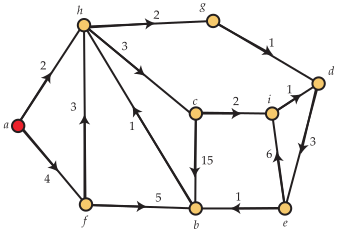
\includegraphics[width=\linewidth]{images/dijkstra_ex2}
\end{image}%
\tcblower
\end{figureptx}%
\end{divisionexercise}%
\begin{divisionexercise}{14}{}{}{g:exercise:idp155}%
\hyperref[x:table:tab_digraph2]{Table~{\xreffont\ref{x:table:tab_digraph2}}} contains the length of the directed edge \((x,y)\) in the intersection of \emph{row} \(x\) and \emph{column} \(y\) in a digraph with vertex set \(\{a,b,c,d,e,f\}\). For example, \(w(b,d)=47\). (On the other hand, \(w(d,b)=6\).) Use this data and Dijkstra's algorithm to find the distance from \(a\) to each of the other vertices and a directed path of that length from \(a\).%
\begin{tableptx}{\textbf{A digraph represented as a table of data}}{x:table:tab_digraph2}{}%
\centering%
{\tabularfont%
\begin{tabular}{lAllllll}
\(w\)&\(a\)&\(b\)&\(c\)&\(d\)&\(e\)&\(f\)\tabularnewline\hrulethin
\(a\)&0&7&17&55&83&42\tabularnewline[0pt]
\(b\)&14&0&13&47&27&17\tabularnewline[0pt]
\(c\)&37&42&0&16&93&28\tabularnewline[0pt]
\(d\)&10&6&8&0&4&32\tabularnewline[0pt]
\(e\)&84&19&42&8&0&45\tabularnewline[0pt]
\(f\)&36&3&76&5&17&0
\end{tabular}
}%
\end{tableptx}%
\end{divisionexercise}%
\begin{divisionexercise}{15}{}{}{g:exercise:idp156}%
Give an example of a digraph having an \emph{undirected} path between each pair of vertices, but having a root vertex \(r\) so that Dijkstra's algorithm cannot find a path of finite length from \(r\) to some vertex \(x\).%
\end{divisionexercise}%
\begin{divisionexercise}{16}{}{}{g:exercise:idp157}%
Notice that in our discussion of Dijkstra's algorithm, we required that the edge weights be nonnegative. If the edge weights are lengths and meant to model distance, this makes perfect sense. However, in some cases, it might be reasonable to allow negative edge weights. For example, suppose that a positive weight means there is a cost to travel along the directed edge while a negative edge weight means that you make money for traveling along the directed edge. In this case, a directed path with positive total weight results in paying out to travel it, while one with negative total weight results in a profit.%
\begin{enumerate}[label=(\alph*)]
\item{}Give an example to show that Dijkstra's algorithm does not always find the path of minimum total weight when negative edge weights are allowed.%
\item{}Bob and Xing are considering this situation, and Bob suggests that a little modification to the algorithm should solve the problem. He says that if there are negative weights, they just have to find the smallest (i.e.\@, most negative weight) and add the absolute value of that weight to every directed edge. For example, if \(w(x,y)\geq -10\) for every directed edge \((x,y)\), Bob is suggesting that they add \(10\) to every edge weight. Xing is skeptical, and for good reason. Give an example to show why Bob's modification won't work.%
\end{enumerate}
%
\end{divisionexercise}%
\end{exercises-section}
\end{chapterptx}
%
%
\typeout{************************************************}
\typeout{Chapter 4 Graphs on Surfaces}
\typeout{************************************************}
%
\begin{chapterptx}{Graphs on Surfaces}{}{Graphs on Surfaces}{}{}{x:chapter:ch_graphs_on_surfaces}
\begin{introduction}{}%
This chapter covers drawing graphs on surfaces. To motivate this topic, we will begin by thinking about videogames%
\par
We start with discussing whether or not graphs are planar, proving that \(K_{3,3}\) and \(K_5\) are not planar using a method we call the Planarity Algorithm for Hamiltonian graphs.  We discuss the more general Kuratowski's theorem for proving any graph is planar or not.  We introduce other surfaces, and how to draw graphs on them -{}-{} the sphere, Mobius band, and torus in particular.  After a brief discussion of dual graphs, we prove Euler's theorem about planar graphs and explore several applications.%
\end{introduction}%
%
%
\typeout{************************************************}
\typeout{Section 4.1 Introduction to Graphs on Surfaces}
\typeout{************************************************}
%
\begin{sectionptx}{Introduction to Graphs on Surfaces}{}{Introduction to Graphs on Surfaces}{}{}{x:section:s_graphs_on_surfaces_intro}
\begin{introduction}{}%
We begin our study of graphs on surfaces with an old chestnut of a problem, the solution of which we will develop into a more general algorithm.%
\end{introduction}%
%
%
\typeout{************************************************}
\typeout{Subsection 4.1.1 The Utilities Problem}
\typeout{************************************************}
%
\begin{subsectionptx}{The Utilities Problem}{}{The Utilities Problem}{}{}{g:subsection:idp158}
Suppose there are three houses, owned by Alice, Bob, and Carol, and they'd each like to be connected to one of three Utilities, say, gas, electricity, and water.  There is no real difficulty in the real world, but if we add the restriction that we don't want any of the lines to cross over or under each other, the problem becomes quite interesting.  A failed attempt at drawing a solution is shown here.%
\begin{figureptx}{An attempt at solving the three utilities problem}{x:figure:failed_utilities}{}%
\begin{image}{0.15}{0.7}{0.15}%
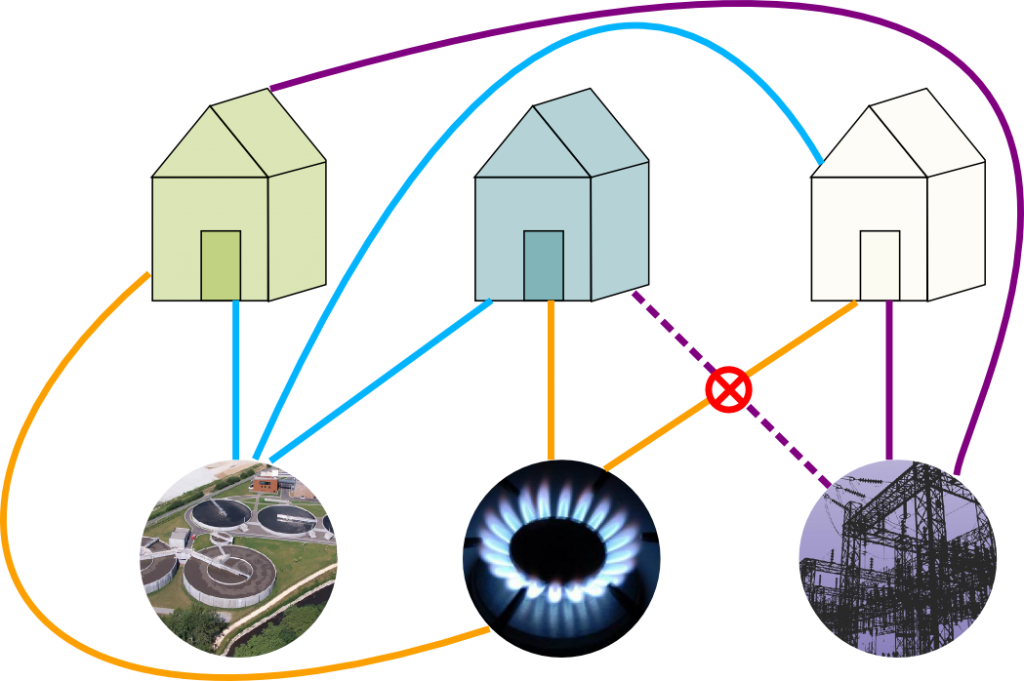
\includegraphics[width=\linewidth]{images/The-Utilities-Problem-Bad-Solution.png}
\end{image}%
\tcblower
\end{figureptx}%
Although this attempt failed, it seems very difficult to rule out that some other attempt wouldn't succeed; trying to make a case by case argument seems quite difficult to organize, and it's not clear that there are even finitely many possibilities.  We need a careful way to approach the problem, which we will do in a moment, but first we will use this problem as motivation to make a few definitions.%
\end{subsectionptx}
%
%
\typeout{************************************************}
\typeout{Subsection 4.1.2 }
\typeout{************************************************}
%
\begin{subsectionptx}{}{}{}{}{}{g:subsection:idp159}
\begin{definition}{}{g:definition:idp160}%
A graph is \emph{planar} if it can be drawn on a piece of paper so that no edges cross.%
\end{definition}
That definition is a bit loose -{}-{} for instance, it's left implicit, we're drawing the edges as lines, with the endpoints being the two vertices it connects.  But this will be strong enough for our purposes.%
\par
With this definition in hand, the Utilities Question is asking whether the graph \(K_{3,3}\) is planar -{}-{} treat the three utilities as red vertices, say, and the three houses as the blue vertices.  This doesn't really help us organize our proof, however. To do that, we will use the basic fact that any circle drawn on the plane has an inside and an outside.%
\par
This last fact sounds absolutely trivial, but first, it is not true on other surfaces, for instance, on the torus -{}-{} in our video game world, the top of the screen makes a circle, but a point just above this circle is really at the bottom of the video game world, and so the circle doesn't cut the torus into two pieces; I also illustrated this with the Mobius band: the central line down the middle doesn't separate it into two pieces.  This fact is usually stated as follows:%
\begin{theorem}{Jordan Curve Theorem.}{}{g:theorem:idp161}%
Any simple closed plane curve has an interior and an exterior%
\end{theorem}
Though easy to state, and intuitively obvious, the Jordan Curve Theorem is surprisingly subtle and difficult to prove; we won't use any more topology than this.%
\par
Before seeing it in practice, let's discuss informally how the Jordan Curve Theorem can be used to help prove whether a graph \(G\) is planar or not.  Suppose that we have found a large cycle \(C_k\) as a subgraph of \(G\).  Then, if we had a planar drawing of \(G\), this cycle would have to appear as a circle.  By the Jordan Curve Theorem, this circle would have an inside and an outside, and every vertex and edge not in our cycle \(C_k\) would have to be either entirely within the circle, or entirely outside the circle.  This gives us a way to organize the case by case argument.%
\par
The bigger a cycle we can find, the fewer other vertices and edges we need to consider, and so we have a much cleaner case by case argument.  In the best cases, the graph is Hamiltonian and the cycle \(C_k\) includes all the vertices of \(G\), and we only have to do a case by case analysis for some the remaining edges.%
\par
Let's see how this general principle gets illustrated in practice%
\begin{theorem}{}{}{g:theorem:idp162}%
\(K_{3,3}\) isn't planar\end{theorem}
\begin{proof}{}{g:proof:idp163}
First let's name the vertices of \(K_{3,3}\): let the vertices \(a,b,c\) be the blue circle vertices, and \(x,y,z\) be the red rectangle vertices.  Then the path \(a-x-b-y-c-z-a\) is a Hamiltonian cycle, and so if \(K_{3,3}\) were planar it would be drawn as a circle in the plane, as shown below:%
\begin{figureptx}{The Hamiltonian cycle in \(K_{3,3}\)}{x:figure:fig_proof_k33_planar1}{}%
\begin{image}{0.15}{0.7}{0.15}%
\resizebox{\linewidth}{!}{%
\begin{tikzpicture}[scale=.7]
\tikzstyle{vertex}=[draw, minimum size=17pt, inner sep=0pt]
\node[circle, vertex, blue] (a) at (0,1) {$a$};
\node[rectangle, vertex, red] (x) at (1,2) {$x$};
\node[circle, vertex, blue] (b) at (3,2) {$b$};
\node[rectangle, vertex, red] (y) at (4,1) {$y$};
\node[circle, vertex, blue] (c) at (3,0) {$c$};
\node[rectangle, vertex,red] (z) at (1,0) {$z$};

\path 
(a) edge (x)
    edge (z)
(b) edge (x)
    edge (y)
(c) edge (z)
    edge (y);
\end{tikzpicture}
}%
\end{image}%
\tcblower
\end{figureptx}%
This contains 6 of the 9 edges of \(K_{3,3}\); we need to add the edges \(a-y, b-z\) and \(c-x\).  The edge \(a-y\) could be drawn inside the circle or outside, suppose we draw it inside, as shown below, with the added edge dashed.%
\begin{figureptx}{Adding \(a-y\) inside}{x:figure:fig_proof_k33_planar2}{}%
\begin{image}{0.15}{0.7}{0.15}%
\resizebox{\linewidth}{!}{%
\begin{tikzpicture}[scale=.7]
\tikzstyle{vertex}=[draw, minimum size=17pt, inner sep=0pt]
\node[vertex, circle, blue] (a) at (0,1) {$a$};
\node[vertex, rectangle, red] (x) at (1,2) {$x$};
\node[vertex, circle, blue] (b) at (3,2) {$b$};
\node[vertex, rectangle, red] (y) at (4,1) {$y$};
\node[vertex, circle, blue] (c) at (3,0) {$c$};
\node[vertex, rectangle, red] (z) at (1,0) {$z$};

\path 
(a) edge (x)
    edge (z)
    edge[dashed] (y)
(b) edge (x)
    edge (y)
(c) edge (z)
    edge (y);
\end{tikzpicture}
}%
\end{image}%
\tcblower
\end{figureptx}%
Then on the inside of the circle, \(x\) and \(c\) are on different sides of the line \(a-y\), and so the edge connecting them must go outside the circle.  The added edge could go around the right of the circle, as shown below here:%
\begin{figureptx}{Adding \(a-y\) inside}{x:figure:fig_proof_k33_planar3}{}%
\begin{image}{0.15}{0.7}{0.15}%
\resizebox{\linewidth}{!}{%
\begin{tikzpicture}[scale=.7]
\tikzstyle{vertex}=[draw, minimum size=17pt, inner sep=0pt]
\clip (-1,-1)--(-1,4)--(5,4)--(5,-1)--cycle;

\node[vertex, circle, blue] (a) at (0,1) {$a$};
\node[vertex, rectangle, red] (x) at (1,2) {$x$};
\node[vertex, circle, blue] (b) at (3,2) {$b$};
\node[vertex, rectangle, red] (y) at (4,1) {$y$};
\node[vertex, circle, blue] (c) at (3,0) {$c$};
\node[vertex, rectangle, red] (z) at (1,0) {$z$};

\path 
(a) edge (x)
    edge (z)
    edge[dashed] (y)
(b) edge (x)
    edge (y)
(c) edge (z)
    edge (y)
    edge[bend right=130, looseness=3, dashed] (x);

\end{tikzpicture}
}%
\end{image}%
\tcblower
\end{figureptx}%
or around the left, as shown here:%
\begin{figureptx}{Adding \(a-y\) inside}{x:figure:fig_proof_k33_planar4}{}%
\begin{image}{0.15}{0.7}{0.15}%
\resizebox{\linewidth}{!}{%
\begin{tikzpicture}[scale=.7]
\tikzstyle{vertex}=[draw, minimum size=17pt, inner sep=0pt]
\clip (-1,-2)--(-1,3)--(5,3)--(5,-2)--cycle;

\node[vertex, circle, blue] (a) at (0,1) {$a$};
\node[vertex, rectangle, red] (x) at (1,2) {$x$};
\node[vertex, circle, blue] (b) at (3,2) {$b$};
\node[vertex, rectangle, red] (y) at (4,1) {$y$};
\node[vertex, circle, blue] (c) at (3,0) {$c$};
\node[vertex, rectangle, red] (z) at (1,0) {$z$};

\path 
(a) edge (x)
    edge (z)
    edge[dashed] (y)
(b) edge (x)
    edge (y)
(c) edge (z)
    edge (y)
    edge[bend left=130, looseness=3, dashed] (x);

\end{tikzpicture}
}%
\end{image}%
\tcblower
\end{figureptx}%
But now \(b\) and \(z\) are different sides of \(a-y\) inside the circle, and on different sides of \(c-x\) outside the circle, and so cannot be connected without making two edges cross.%
\par
If we had began by drawing \(a-y\) outside the circle, then we would have had to draw \(c-x\) inside the circle, and had the same problem with being able to draw the last line; as shown here:%
\begin{figureptx}{Adding \(a-y\) inside}{x:figure:fig_proof_k33_planar5}{}%
\begin{image}{0.15}{0.7}{0.15}%
\resizebox{\linewidth}{!}{%
\begin{tikzpicture}[scale=.7]
\tikzstyle{vertex}=[draw, minimum size=17pt, inner sep=0pt]
\clip (-1,-1)--(-1,4)--(5,4)--(5,-1)--cycle;

\node[vertex, circle, blue] (a) at (0,1) {$a$};
\node[vertex, rectangle, red] (x) at (1,2) {$x$};
\node[vertex, circle, blue] (b) at (3,2) {$b$};
\node[vertex, rectangle, red] (y) at (4,1) {$y$};
\node[vertex, circle, blue] (c) at (3,0) {$c$};
\node[vertex, rectangle, red] (z) at (1,0) {$z$};

\path 
(a) edge (x)
    edge (z)
    edge[dashed, bend left=90, looseness=1.5] (y)
(b) edge (x)
    edge (y)
(c) edge (z)
    edge (y)
    edge[dashed] (x);

\end{tikzpicture}
}%
\end{image}%
\tcblower
\end{figureptx}%
\end{proof}
\end{subsectionptx}
\end{sectionptx}
%
%
\typeout{************************************************}
\typeout{Section 4.2 The planarity algorithm for Hamiltonian graphs}
\typeout{************************************************}
%
\begin{sectionptx}{The planarity algorithm for Hamiltonian graphs}{}{The planarity algorithm for Hamiltonian graphs}{}{}{x:section:s_graphs_on_surfaces_planarity_algorithm}
\begin{introduction}{}%
In the previous chapter we showed that \(K_{3,3}\) isn't planar; in this section we investigate how the ideas we used to solve the utilities problem for \(K_{3,3}\)-{}-{} namely, the Jordan Curve theorem and the fact that \(K_{3,3}\) is Hamiltonian -{}-{} generalize to other graphs.  In the end, this will culminate in "The Planarity Algorithm for Hamiltonian Graphs".%
\end{introduction}%
%
%
\typeout{************************************************}
\typeout{Subsection 4.2.1 Stereographic Projection and Unnecessary cases}
\typeout{************************************************}
%
\begin{subsectionptx}{Stereographic Projection and Unnecessary cases}{}{Stereographic Projection and Unnecessary cases}{}{}{g:subsection:idp164}
It will make our life easier if before we investigate other graphs we streamline our proof for \(K_{3,3}\) slightly: there were a few times where we had to treat different cases that wound up behaving essentially the same, and we'd like to see that we didn't actually need to treat them as separate cases.  In particular, we would like to show that the following three seemingly different ways to connect the first two vertices lead to the same analysis:%
\begin{enumerate}
\item{}Connecting them inside the Hamiltonian cycle%
\item{}Connecting them outside "to the left"%
\item{}Connecting them outside "to the right"%
\end{enumerate}
%
\begin{figureptx}{The three cases}{x:figure:fig_inside_outside}{}%
\begin{image}{0.15}{0.7}{0.15}%
\resizebox{\linewidth}{!}{%
\begin{tikzpicture}[scale=.7]
\tikzstyle{vertex}=[circle, draw, minimum size=17pt, inner sep=0pt]
\node[vertex] (a) at (0,1) {};
\node[vertex] (x) at (1,2) {};
\node[vertex] (b) at (3,2) {};
\node[vertex] (y) at (4,1) {};
\node[vertex] (c) at (3,0) {};
\node[vertex] (z) at (1,0) {};

\path 
(a) edge (x)
    edge (z)
    edge[dashed] (y)
(b) edge (x)
    edge (y)
(c) edge (z)
    edge (y);

\begin{scope}[xshift=5cm]
\node[vertex] (a) at (0,1) {};
\node[vertex] (x) at (1,2) {};
\node[vertex] (b) at (3,2) {};
\node[vertex] (y) at (4,1) {};
\node[vertex] (c) at (3,0) {};
\node[vertex] (z) at (1,0) {};

\path 
(a) edge (x)
    edge (z)
    edge[bend right=225, looseness=3, dashed] (y)
(b) edge (x)
    edge (y)
(c) edge (z)
    edge (y);

\end{scope}

\begin{scope}[xshift=10cm]
\node[vertex] (a) at (0,1) {};
\node[vertex] (x) at (1,2) {};
\node[vertex] (b) at (3,2) {};
\node[vertex] (y) at (4,1) {};
\node[vertex] (c) at (3,0) {};
\node[vertex] (z) at (1,0) {};

\path 
(a) edge (x)
    edge (z)
    edge[bend left=225, looseness=3, dashed] (y)
(b) edge (x)
    edge (y)
(c) edge (z)
    edge (y);

\end{scope}

\end{tikzpicture}
}%
\end{image}%
\tcblower
\end{figureptx}%
The solution will be to think about drawing the graphs on the sphere \(S^2\) instead of the plane.  First, let's see why this solves our problem.  On the plane, the inside of a circle is different from the outside of a circle -{}-{} the inside is bounded, but the outside is unbounded.  However, on the sphere, the two sides of a circle are equivalent -{}-{} you can deform any circle to be an equator, and then the northern hemisphere is equivalent to the southern hemisphere. This shows on there sphere, the inside and the outside aren't really different cases.%
\par
Furthermore, going around the outside to "the left" or "to the right" are equivalent on the sphere -{}-{} you can slowly make the path around the sphere bigger and bigger, and then slip it around the north or south pole, and back.  Alternatively, we've already seen that the inside of the circle is equivalent to the outside of the circle on the sphere \(S^2\), and on the inside of the circle it doesn't matter exactly how the two points are connected, and so it shouldn't matter on the outside, either.%
\par
So we've argued that if we're trying to draw a graph on the sphere, all three cases are the same, but it should still feel like a bait-and-switch: we weren't trying to draw graphs on there sphere, we were trying to draw graphs on the plane.  The connection comes from the fact that the sphere can be viewed as a plane with one additional point.%
\begin{proposition}{}{}{g:proposition:idp165}%
Let \(p\in S^2\) be any point.  Then \(S^2\setminus\{p\}\cong\reals^2\).\end{proposition}
\begin{proof}{}{g:proof:idp166}
One way to visualize this is imagine the sphere as being made from very flexible clay.  If we poke a small hole in the top of the sphere, we could stick our fingers in and make the hole larger, and gradually stretch and bend and reform for the sphere to be a flat disk, which could be stretched to be the whole plane, in the same way the tangent function maps the interval \((-\pi/2, pi/2)\) to the whole real line \(\reals\)%
\par
Alternatively, one could use stereographic projection, as shown in Figure .  Draw \(S^2\) in \(\reals^3\) as the unit sphere at the origin, and let \(N=(0,0,1)\) be the north pole of the sphere.  Stereographic projection gives a bijection between \(S^2\setminus\{N\}\) (the sphere minus the north pole) to the plane, as follows: for any point \(p\neq N\) the line through \(p\) and \(N\) must meet the \(xy\)-plane at one point.  On the other hand, any line through \(N\) and a point on the \(xy\)-plane must meet the sphere at one other point.%
\begin{figureptx}{Stereographic Projection}{x:figure:img-stereographic}{}%
\begin{image}{0.05}{0.9}{0.05}%
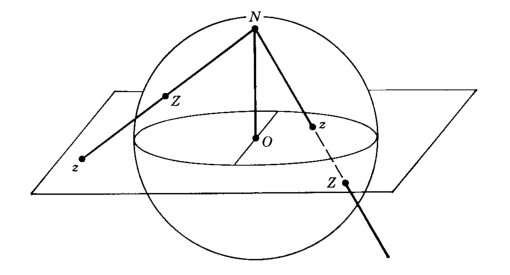
\includegraphics[width=\linewidth]{images/stereographic.jpg}
\end{image}%
\tcblower
\end{figureptx}%
Accepting that \(S^2\) is \(\reals^2\) minus one point, we see that we can draw a given graph \(\bfG\) on \(S^2\) if and only if we can draw \(\bfG\) on \(\reals^2\): if we draw it on \(\reals^2\), we can view the \(\reals^2\) as a small patch of \(S^2\). And if we have a drawing on \(S^2\), there must be at least one point on \(S^2\) that isn't in the drawing of \(G\), and doing stereographic projection from that point gives a drawing of \(G\) on the plane \(\reals^2\).%
\end{proof}
\end{subsectionptx}
%
%
\typeout{************************************************}
\typeout{Subsection 4.2.2 The planarity algorithm}
\typeout{************************************************}
%
\begin{subsectionptx}{The planarity algorithm}{}{The planarity algorithm}{}{}{g:subsection:idp167}
The preceeding discussion may have felt heavy going, but the upshot is that the cases that seemed "the same" in our analysis of \(K_{3,3}\) actually are the same, and similar cases will be the same for any graph. This will make it much easier to extend our reasoning to more complicated graphs.%
\par
Suppose that \(G\) is Hamiltonian, and choose a Hamiltonian cycle; if \(G\) were planar than this cycle must be drawn as a circle, and every other edge must either lie entirely inside or entirely outside the graph.  Now consider two edges \(e=ab\) and \(f=xy\) that are not part of the cycle.  Depending on the order that \(a,b,x\) and \(y\) appear as you go around the Hamiltonian cycle, one of two things will happen:%
\begin{enumerate}
\item{}If the vertices of \(e\) and \(f\) do not interlace (e.g. \(abxy, yxab, xbay,\cdots\)), or if they share a vertex (e.g., \(a=x\)), then \(e\) may be drawn both inside or both outside the circle without crossing%
\item{}If the vertices of \(e\) and \(f\) do interlace (e.g. \(axby, xayb, yaxb,\dots...\)) then if \(e\) and \(f\) are drawn both inside or both outside the circle, they must cross%
\end{enumerate}
%
\par
This motivates the following definition%
\begin{definition}{Cross(\(G,C\)).}{g:definition:idp168}%
Let \(G\) be a Hamiltonian graph, and \(C\) a Hamiltonian cycle in \(G\).  The \emph{crossing graph} of \(G\) and \(C\), denoted Cross(\(G,C\)) has as vertices the edges of \(G\) that aren't in the cycle, and an edge between vertices \(p\) and \(q\) if the vertices of the corresponding edges interleave -{}-{} that is, \(p\) and \(q\) are adjacent if they cannot be drawn on the same side of the cycle \(C\) without crossing.%
\end{definition}
\begin{algorithm}{The planarity algorithm for complete graphs.}{}{g:algorithm:idp169}%
Suppose that \(G\) is Hamiltonian, and \(C\) is a Hamiltonian cycle.  Then \(G\) is planar if and only if Cross(\(G,C\)) is bipartite.%
\end{algorithm}
The idea is that if \(G\) is planar, the vertices of Cross(\(G,C\)) are naturally bicolored, with the red vertices, say, corresponding to the edges that are drawn inside the cycle \(C\), and the blue edge corresponding to the edges that are drawn outside the cycle \(C\).  The definition of the edges of Cross(\(G,C\)) guarantees there are no edges between vertices of the same color.%
\par
Similarly, if we can find a colouring of the vertices of Cross(\(G,C\)) so that adjacent vertices have different colours, then we can draw all the edges of \(G\) corresponding to red vertices of Cross(\(G,C\)) inside (or outside) \(C\) without having any of them cross.%
\begin{example}{The complete graph \(K_5\) isn't planar.}{g:example:idp170}%
Let's apply the planarity algorithm to the complete graph \(K_5\).  Let's label the vertices 1-5, and take our Hamiltonian cycle \(C\) to be 123451, which we've drawn as the outside pentagon in the following figure: \begin{figureptx}{The graph (\(K_5\))}{x:figure:fig_planarity_crossk5_edge13}{}%
\begin{image}{0.15}{0.7}{0.15}%
\resizebox{\linewidth}{!}{%
\begin{tikzpicture}[scale=.7]
\tikzstyle{vertex}=[circle, draw, minimum size=17pt, inner sep=0pt]
\node[vertex] (1) at (1,0) {$1$};
\node[vertex] (2) at (0,2) {$2$};
\node[vertex] (3) at (2,3) {$3$};
\node[vertex] (4) at (4,2) {$4$};
\node[vertex] (5) at (3,0) {$5$};


\path 
(1) edge (2)
    edge (3)
    edge (4)
    edge (5)
(2) edge (3)
    edge (4)
    edge (5)
(3) edge (4)
    edge (5)
(4) edge (5);

\end{tikzpicture}
}%
\end{image}%
\tcblower
\end{figureptx}%
 Since \(K_5\) has \(\binom{5}{2}=10\) vertices, there are 5 edges that aren't used in \(C\), namely 13,14, 24,25, and 35.  So Cross(\(K_5, 123451\)) will consist of these five vertices.  We see that 13 will be adjacent to 24 and 25, since these edges would cross if drawn inside, but 13 is not adjacent to 14 or 35, since these edges would cross 13 if drawn on the same side of the circle, as illustrated in the next figure%
\begin{figureptx}{The edges 13 does and does not cross}{x:figure:fig_planarity_crossk5edges}{}%
\begin{image}{0.15}{0.7}{0.15}%
\resizebox{\linewidth}{!}{%
\begin{tikzpicture}[scale=.7]
\tikzstyle{vertex}=[circle, draw, minimum size=17pt, inner sep=0pt]


\node[vertex] (1) at (1,0) {$1$};
\node[vertex] (2) at (0,2) {$2$};
\node[vertex] (3) at (2,3) {$3$};
\node[vertex] (4) at (4,2) {$4$};
\node[vertex] (5) at (3,0) {$5$};
\path 
(1) edge (2)
    edge (3)
    edge (5)
(2) edge (3)
    edge (4)
(3) edge (4)
(4) edge (5);


\begin{scope}[yshift=-5cm]
\node at (2,-1) {13 crosses 24 and 25};
\node[vertex] (1) at (1,0) {$1$};
\node[vertex] (2) at (0,2) {$2$};
\node[vertex] (3) at (2,3) {$3$};
\node[vertex] (4) at (4,2) {$4$};
\node[vertex] (5) at (3,0) {$5$};
\path 
(1) edge (2)
    edge (3)
    edge (5)
(2) edge (3)
    edge (5)
(3) edge (4)
(4) edge (5);
\end{scope}


\begin{scope}[xshift=8cm]
\node[vertex] (1) at (1,0) {$1$};
\node[vertex] (2) at (0,2) {$2$};
\node[vertex] (3) at (2,3) {$3$};
\node[vertex] (4) at (4,2) {$4$};
\node[vertex] (5) at (3,0) {$5$};
\path 
(1) edge (2)
    edge (3)
    edge (4)
    edge (5)
(2) edge (3)
(3) edge (4)
(4) edge (5);


\begin{scope}[yshift=-5cm]
\node at (2,-1) {13 doesn't cross 14 or 35};
\node[vertex] (1) at (1,0) {$1$};
\node[vertex] (2) at (0,2) {$2$};
\node[vertex] (3) at (2,3) {$3$};
\node[vertex] (4) at (4,2) {$4$};
\node[vertex] (5) at (3,0) {$5$};
\path 
(1) edge (2)
    edge (3)
    edge (5)
(2) edge (3)
(3) edge (4)
    edge (5)
(4) edge (5);
\end{scope}




\end{scope}

\end{tikzpicture}
}%
\end{image}%
\tcblower
\end{figureptx}%
Similar consideration with the other edges show that Cross(\(K_5, 123451\)) is the following graph, which is isomorphic to a five cycle:%
\begin{figureptx}{The graph Cross(\(K_5, 123451\))}{x:figure:fig_planarity_crossk5}{}%
\begin{image}{0.15}{0.7}{0.15}%
\resizebox{\linewidth}{!}{%
\begin{tikzpicture}[scale=.7]
\tikzstyle{vertex}=[circle, draw, minimum size=17pt, inner sep=0pt]
\node[vertex] (13) at (1,0) {$13$};
\node[vertex] (14) at (0,2) {$14$};
\node[vertex] (24) at (2,3) {$24$};
\node[vertex] (25) at (4,2) {$25$};
\node[vertex] (35) at (3,0) {$35$};


\path 
(13) edge (24)
    edge (25)
(14) edge (25)
    edge (35)
(24) edge (35);

\end{tikzpicture}
}%
\end{image}%
\tcblower
\end{figureptx}%
In particular, Cross(\(K_5, 123451\)) is not bipartite.  Hence, by the planarity algorithm for Hamiltonian graphs, we see that \(K_5\) is not planar.%
\end{example}
\begin{example}{A planar graph.}{g:example:idp171}%
Let's use the planarity algorithm for Hamiltonian graphs to find a planar drawing of the graph shown in the next figure.%
\begin{figureptx}{A graph \(H\)}{x:figure:fig_planarity_example_mess}{}%
\begin{image}{0.15}{0.7}{0.15}%
\resizebox{\linewidth}{!}{%
\begin{tikzpicture}[scale=.7]
\tikzstyle{vertex}=[circle, draw, minimum size=17pt, inner sep=0pt]
\node[vertex] (b) at (0,1) {$b$};
\node[vertex] (c) at (1,2) {$c$};
\node[vertex] (x) at (3,2) {$x$};
\node[vertex] (y) at (4,1) {$y$};
\node[vertex] (z) at (3,0) {$z$};
\node[vertex] (a) at (1,0) {$a$};

\path 
(a) edge (b)
    edge (x)
    edge (y)
    edge (z)
(b) edge (c)
    edge (x)
    edge (z)
(c) edge (x)
    edge (y)
    edge (z)
(x) edge (y)
(y) edge (z);


\end{tikzpicture}
}%
\end{image}%
\tcblower
\end{figureptx}%
We see that \(H\) is Hamiltonian and take as our Hamiltonian cycle the path around the outside, namely \(abcxyza\).  There are then six edges not contained in the Hamiltonian cycle, and we find that Cross(\(H, abcxyz\)) is as follows:%
\begin{figureptx}{The graph Cross(\(H, abcxyza)\)}{x:figure:fig_planarity_example_cross}{}%
\begin{image}{0.15}{0.7}{0.15}%
\resizebox{\linewidth}{!}{%
\begin{tikzpicture}[scale=.7]
\tikzstyle{vertex}=[circle, draw, minimum size=17pt, inner sep=0pt]
\node[vertex] (ax) at (0,1) {$ax$};
\node[vertex] (cy) at (1,2) {$cy$};
\node[vertex] (bx) at (3,2) {$bx$};
\node[vertex] (cz) at (4,1) {$cz$};
\node[vertex] (ay) at (3,0) {$ay$};
\node[vertex] (bz) at (1,0) {$bz$};

\path 
(ax) edge (bz)
    edge (cy)
    edge (cz)
(bx) edge (cy)
    edge (cz)
(ay) edge (cz)
    edge (bz);
\end{tikzpicture}
}%
\end{image}%
\tcblower
\end{figureptx}%
For instance, in \(H\) the edge \(ax\) crosses the three edges \(cy, cz\) and \(bz\), and so in Cross(\(H, abcxyza\)), the vertex \(ax\) is adjacent to these vertices.%
\par
The graph Cross(\(H, abcxyza)\) has no odd cycles and hence is bipartite -{}-{} for instance, we may color \(ax, bx\) and \(ay\) red, and the other three vertices blue.  Then, to draw \(H\) in the plane without edges crossing, we draw the red edges inside the cycle, and the blue edges outside the cycle:%
\begin{figureptx}{The graph \(H\) drawn without edges crossing}{x:figure:fig_planarity_example_planar_drawing}{}%
\begin{image}{0.15}{0.7}{0.15}%
\resizebox{\linewidth}{!}{%
\begin{tikzpicture}[scale=.7]
\tikzstyle{vertex}=[circle, draw, minimum size=17pt, inner sep=0pt]
\node[vertex] (b) at (0,1) {$b$};
\node[vertex] (c) at (1,2) {$c$};
\node[vertex] (x) at (3,2) {$x$};
\node[vertex] (y) at (4,1) {$y$};
\node[vertex] (z) at (3,0) {$z$};
\node[vertex] (a) at (1,0) {$a$};

\path 
(a) edge (b)
    edge (x)
    edge (y)
    edge (z)
(b) edge (c)
    edge (x)
    edge[bend right=90, looseness=1] (z)
(c) edge (x)
    edge[bend left=90, looseness=1] (y)
    edge[bend left=135, looseness=3] (z)
(x) edge (y)
(y) edge (z);


\end{tikzpicture}
}%
\end{image}%
\tcblower
\end{figureptx}%
\end{example}
\end{subsectionptx}
\end{sectionptx}
%
%
\typeout{************************************************}
\typeout{Section 4.3 Kuratowski's Theorem}
\typeout{************************************************}
%
\begin{sectionptx}{Kuratowski's Theorem}{}{Kuratowski's Theorem}{}{}{x:section:s_graphs_on_surfaces_Kuratowski}
\begin{introduction}{}%
The planrity Algorithm for Hamiltonian graphs gives a very convenient and systematic way to determine whether a Hamiltonian graph is planar or not, and we saw that with some work it can be hacked to work for graphs that are "almost" Hamiltonian -{}-{} that have a cycle that go through all but one or two vertices, say.%
\par
Stretching these ideas further, the general logic of considering cycles and applying the Jordan Curve theorem to them would provide a way to prove whether an abritrary graph is planar or not, but as we have more or more vertices that aren't on our cycle to consider the arguments would get more and more complicated, and it's clear that a better method is desirable.  In this section we will present, (but not completely prove) Kuratowski's theorem, which gives a method to determine whether or not an arbitrary graph is planar.%
\end{introduction}%
%
%
\typeout{************************************************}
\typeout{Subsection 4.3.1 Planarity, subgraphs, and subdivisions}
\typeout{************************************************}
%
\begin{subsectionptx}{Planarity, subgraphs, and subdivisions}{}{Planarity, subgraphs, and subdivisions}{}{}{g:subsection:idp172}
The idea behind Kuratowski's theorem rests on two small observations, which we illustrate in a simple example before discussing more formally.%
\begin{figureptx}{Two nonplanar graphs}{x:figure:fig-K33-subs}{}%
\begin{image}{0.05}{0.9}{0.05}%
\resizebox{\linewidth}{!}{%
\begin{tikzpicture}[scale=.5]
  \draw node at (1,3) {$\mathbf{G}_1$};
   \draw node at (6,3) {$\mathbf{G}_2$};
  

\begin{scope}[every node/.style={circle, draw, fill=red, inner sep=0pt, minimum width=4pt, thick}]
  \draw node (a) at (0,0) {};
o  \draw node (b) at (0,1) {};
  \draw node (c) at (0,2) {};
  \draw node (x) at (2,0) {};
  \draw node (y) at (2,1) {};
  \draw node (z) at (2,2) {};
  \draw node (extra) at (1,-1) {};
  \draw (a)--(x)--(b)--(y)--(c)--(z)--(a)--(y);
  \draw (b)--(z);
  \draw (c)--(x);
  \draw (extra)--(c)--(b); 


  \begin{scope}[xshift=5cm]
  \draw node (a) at (0,0) {};
  \draw node (b) at (0,1) {};
  \draw node (c) at (0,2) {};
  \draw node (x) at (2,0) {};
  \draw node (y) at (2,1) {};
  \draw node (z) at (2,2) {};
  \draw node (extra) at (1,0) {};
  \draw (a)--(extra)--(x)--(b)--(y)--(c)--(z)--(a)--(y);
  \draw (b)--(z);
  \draw (c)--(x);

    \end{scope}
\end{scope}  
\end{tikzpicture}
}%
\end{image}%
\tcblower
\end{figureptx}%
The graphs \(\bfG_1\) and \(\bfG_2\) in \hyperref[x:figure:fig-K33-subs]{Figure~{\xreffont\ref{x:figure:fig-K33-subs}}} both \emph{look} a lot like \(K_{3,3}\), and since \(K_{3,3}\) is nonplanar, we might expect them to be nonplanar as well, but we need to be careful and precise in checking this.  We work this out in the next example.%
\begin{example}{Two nonplanar graphs.}{g:example:idp173}%
The graph \(\bfG_1\) in \hyperref[x:figure:fig-K33-subs]{Figure~{\xreffont\ref{x:figure:fig-K33-subs}}} is \(K_{3,3}\) with a vertex and two edges added to it; put another way, \(K_{3,3}\) is a subgraph of \(\bfG_1\).  If we could draw \(\bfG_1\) in the plane, we could just ignore this extra vertex and these two edges, and we'd have a drawing of \(K_{3,3}\) in the plane, but we know \(K_{3,3}\) isn't planar.  So to avoid contradictions we are forced to conclude that \(\bfG_1\) isn't planar.%
\par
The graph \(\bfG_2\) looks just like \(K_{3,3}\), but we have added an extra vertex of degree two in the middle of one of the edges.  Note that \(K_{3,3}\) is \emph{not} a subgraph of \(\bfG_2\), and so we need to use slightly different reasoning than we did for showing \(\bfG\) isn't planar.  But drawing \(\bfG_2\) is just like drawing \(K_{3,3}\) and then adding an extra dot for the new vertex of degree two.  If we could draw \(\bfG_2\) in the plane, we could just skip adding this extra dot, and we'd have a drawing of \(K_{3,3}\) in the plane.  Again, since we know \(K_{3,3}\) isn't planar, we see that \(\bfG_2\) isn't planar, either.%
\end{example}
We will now generalize the methods we used to show \(\bfG\) and \(\bfH\) are nonplanar and summarize them as lemmas.  The reasoning we used to prove that \(\bfG\) was nonplanar doesn't need to be changed at all to prove:%
\begin{lemma}{}{}{x:lemma:lemma-nonplanar-subgraph}%
If \(\bfH\) is nonplanar, and \(\bfH\) is a subgraph of \(\bfG\), then \(\bfG\) isn't planar.\end{lemma}
\begin{proof}{}{g:proof:idp174}
We've essentially already proved it, but we'll restate the reasoning in a different way for completeness.%
\par
When we draw a graph \(\bfG\) in the plane, we also draw all the subgraphs of \(\bfG\) in the plane.  Thus, if \(\bfG\) is planar, then all of its subgraphs are planar.  Our lemma is the contrapositive of this statement.%
\end{proof}
\hyperref[x:lemma:lemma-nonplanar-subgraph]{Lemma~{\xreffont\ref{x:lemma:lemma-nonplanar-subgraph}}} is logically equivalent to the discussion above, but it's worth restating the logic in this direction as well: if we can't draw \(\bfG\) in the plane, then we certainly can't draw \(\bfH\) in the plane without edges crossing, as if we could then we'd have a drawing of \(\bfH\) as part of our big drawing.%
\begin{example}{Complete graphs.}{g:example:idp175}%
If \(n\gt 5\), then \(K_n\) is not planar by \hyperref[x:lemma:lemma-nonplanar-subgraph]{Lemma~{\xreffont\ref{x:lemma:lemma-nonplanar-subgraph}}}, because \(K_5\) is a subgraph of \(K_n\), and we know that \(K_5\) isn't planar.%
\par
We could also have used the fact that \(K_{3,3}\) is a subgraph of \(K_n\), and \(K_{3,3}\) is also nonplanar.%
\end{example}
To generalize the method we used to prove \(\bfG_2\) is non-planar, we first make a form definition that encapsulates the idea of "adding dots" to the middle of edges:%
\begin{definition}{Subdivision.}{g:definition:idp176}%
We say that \(\bfG\) is a \emph{subdivision} of \(\bfH\) if \(\bfG\) is obtained from \(\bfH\) by adding some vertices of degree two in the middle of some of the edges of \(\bfH\).%
\end{definition}
\begin{example}{Cycles and Paths.}{g:example:idp177}%
Any path graph \(P_n, n\geq 2\) is a subdivision of the graph \(P_2\) consisting of two vertices with an edge between them.  Any cycle graph \(C_m, m\geq 3\) is a subdivision of the triangle \(C_3\)%
\end{example}
\begin{lemma}{}{}{x:lemma:lemma-nonplanar-subdivision}%
If \(\bfG\) is a subdivision of a nonplanar graph \(\bfH\), then \(\bfG\) is nonplanar.%
\end{lemma}
\begin{proof}{}{g:proof:idp178}
Suppose that \(\bfG\) was planar, and draw it in the graph.  Then erase the, vertices of degree we added when we subdivided \(\bfH\), merging the edges on either side to one.  We obtain a planar drawing of \(\bfH\), a contradiction, and so \(\bfG\) must not have been planar.%
\end{proof}
\end{subsectionptx}
%
%
\typeout{************************************************}
\typeout{Subsection 4.3.2 Kuratowski's Theorem}
\typeout{************************************************}
%
\begin{subsectionptx}{Kuratowski's Theorem}{}{Kuratowski's Theorem}{}{}{g:subsection:idp179}
The definitions and lemma of the previous section essentially prove the "easy" direction of the following theorem, which will be our main tool for proving graphs aren't planar.%
\begin{theorem}{Kuratowski's Theorem.}{}{g:theorem:idp180}%
A graph \(\bfG\) is nonplanar if and only if \(\bfG\) has a subgraph that's a subdivision of \(K_{3,3}\) or \(K_5\).%
\end{theorem}
\begin{proof}{}{g:proof:idp181}
We will only prove one direction: that if \(\bfG\) has such a subgraph, then \(\bfG\) is nonplanar; the other direction is more difficult.%
\par
Suppose that \(\bfH\) is a subgraph of \(\bfG\) that is subdivision of \(K_{3,3}\) or \(K_5\).  Since we've proven \(K_{3,3}\) and \(K_5\) are nonplanar, we know \(\bfH\) is nonplanar by \hyperref[x:lemma:lemma-nonplanar-subdivision]{Lemma~{\xreffont\ref{x:lemma:lemma-nonplanar-subdivision}}}.  Now since we \(\bfH\) is a subgraph of \(\bfG\) and we know \(\bfH\) is nonplanar, we know \(\bfG\) is nonplanar by \hyperref[x:lemma:lemma-nonplanar-subgraph]{Lemma~{\xreffont\ref{x:lemma:lemma-nonplanar-subgraph}}}.%
\end{proof}
Although we've only proven one direction of Kuratowski's theorem, it's the important direction -{}-{} the one that lets us prove graphs are nonplanar.  The other direction would tell us information about subgraphs of a graph that we already knew was nonplanar for some other reason.  Or, taking the contrapositive, it would let us prove a graph \emph{was} planar by looking at all subgraphs of it and showing none of them looked like \(K_5\) or \(K_{3,3}\).  But this would be a lot of work and there's a much easier way to show a graph is planar: draw it in the plane! If you're asked to prove a graph is planar, you will almost always also be asked to draw it in the plane.%
\par
However, we will \emph{implicitly} use the hard direction in the following way: if a graph \(\bfG\) is nonplanar, you can \emph{always} use Kuratowski's theorem to prove that it's nonplanar.  This is reassuring because it means our tool will always work to prove it's nonplanar, and that you aren't wasting your time looking for subgraphs that don't exist.%
\end{subsectionptx}
%
%
\typeout{************************************************}
\typeout{Subsection 4.3.3 Applying Kuratowski's Theorem}
\typeout{************************************************}
%
\begin{subsectionptx}{Applying Kuratowski's Theorem}{}{Applying Kuratowski's Theorem}{}{}{g:subsection:idp182}
The tricky part of using Kuratowski's theorem is actually \emph{finding} the desired subgraph.  We won't really discuss algorithm aspects of this; for any graph you are asked to prove non-planar, it will be possible to do so by educated trial an error.  A few rules of thumb may be helpful, however.  First, note that subdivision cannot increase the degree of any vertex.  So, for \(\bfG\) to have a subgraph that's a subdivision of \(K_5, \bfG\) has to have at least 5 vertice with degree at least 4; if it doesn't, but we still suspect \(\bfG\) to be nonplanar, we know instead that we should be looking for a subdivision of \(K_{3,3}\).%
\par
Conceptually, it can be useful to think that some vertices of \(\bfG\) are going to be vertices of your \(K_5\) or \(K_{3,3}\), and we're going to need to connect those.  We can use the remaining vertices of \(\bfG\) as parts of subdivided edges between these, but these extra vertices can only be used in at most one such connection.  Thus, these extra vertices are a limited resource we have, and a useful heuristic in looking for subgraph is to take a "greedy" approach, where we choose our vertices to require as few subdivisions as possible to make connections.  We illustrate this idea in the next example.%
\begin{example}{The Petersen graph isn't planar.}{g:example:idp183}%
\begin{figureptx}{The Petersen graph, labeled}{x:figure:fig-Petersen-labeled}{}%
\begin{image}{0.05}{0.9}{0.05}%
\resizebox{\linewidth}{!}{%
\begin{tikzpicture}

\foreach \x in {1,..., 5} \draw node (\x) at (162-72*\x:4) {\x};
\foreach \x in {6,..., 10} \draw node (\x) at (162-72*\x:2) {\x};
\draw[thin, dotted] (1)--(2)--(3)--(4)--(5)--(10)--(8)--(3);
\draw[thin, dotted] (5)--(1)--(6)--(9)--(4);
\draw[thin, dotted] (2)--(7)--(10)--(8)--(6);
\draw[thin, dotted] (7)--(9);

\end{tikzpicture}
}%
\end{image}%
\tcblower
\end{figureptx}%
Let us use Kuratowski's Theorem to prove that the Petersen graph isn't planar; \hyperref[x:figure:fig-Petersen-labeled]{Figure~{\xreffont\ref{x:figure:fig-Petersen-labeled}}} has a drawing of the Petersen graph with the vertices labeled for referece.  Since the Petersen graph is regular of degree three, we know that it can't have a subgrpah that's a subdivision of \(K_5\), as it would need to have some vertices of degree 4 or larger.%
\par
It makes sense to attempt a greedy algorithm -{}-{} in the standard drawing of the Petersen grpah, pick the very top vertex 1 to be "red" and the three vertices adjacent to it to, 2, 5, and 6, to be "blue".  We need two more red vertices.  All vertices left are adjacent to exactly one blue vertex, so from a greedy point of view there is no preference for which vertex we pick to be the next blue vertex.  Let us pick 9 to be another red vertex.  Then it is connected directly to blue vertex 6, but we must find paths from 9 to 2 and 5.  We could, for instance, take the path 9-4-3-2 to connect to 2, but that would use two vertices up while the path 9-7-2 only uses one extra vertex, and so seems better.  Then we can connected 9 to 5 through vertex 4, and vertex 9 has been connected to all the blue vertices.%
\par
Now, we need to choose one more vertex to be a red vertex, and the vertices we haven't used are 3, 10, and 8.  If we tried to make 3 the last red vertex we run into a problem: we need to connect vertex 3 to 3 other vertices, but one of the edges goes to vertex 4 which was one of the subdivided vertices that we can't visit again.  Hence, we only have two possible paths out of 3, and will ever only be able to connect it to two blue vertices.  A similar problem occurs if we try to make 10 the last red vertex -{}-{} it's adjacent to the vertex 7 used as a subdivided vertex.  The remaining choice is vertex 8, which works, as shown in the following diagram.%
\begin{figureptx}{A subdivided \(K_{3,3}\) in the Petersen graph}{x:figure:fig-Petersen-nonplanar}{}%
\begin{image}{0.05}{0.9}{0.05}%
\resizebox{\linewidth}{!}{%
\begin{tikzpicture}

\foreach \x in {1,..., 5} \draw node (\x) at (162-72*\x:4) {\x};
\foreach \x in {6,..., 10} \draw node (\x) at (162-72*\x:2) {\x};
\draw[thin, dotted] (1)--(2)--(3)--(4)--(5)--(10)--(8)--(3);
\draw[thin, dotted] (5)--(1)--(6)--(9)--(4);
\draw[thin, dotted] (2)--(7)--(10)--(8)--(6);
\draw[thin, dotted] (7)--(9);

\node at (90:4) [red, rectangle, draw] (r1) {1};
\node at (234:2) [red, rectangle, draw] (r9) {9};
\node at (306:2) [red, rectangle, draw] (r8) {8};


\node at (18:4) [blue, circle, draw] (b2) {2};
\node at (90:2) [blue, circle, draw] (b6) {6}; 
\node at (162:4) [blue, circle, draw] (b5) {5};

\draw[thick] (r1)--(b5)--(10)--(r8)--(b6)--(r9)--(7)--(b2)--(1);
\draw[thick] (r1)--(b6);
\draw[thick] (b5)--(4)--(r9);
\draw[thick] (b2)--(3)--(r8);

\end{tikzpicture}
}%
\end{image}%
\tcblower
\end{figureptx}%
The red and blue vertices of the subdivided \(K_{3,3}\) are shown as squares\slash{}circles, and the edges of the subdivided \(K_{3,3}\) are colored thick -{}-{} only the dotted edges 7-10 and 3-4 of the Petersen graph are not used in the subgraph.%
\end{example}
\end{subsectionptx}
\end{sectionptx}
%
%
\typeout{************************************************}
\typeout{Section 4.4 Drawing Graphs on Other surfaces}
\typeout{************************************************}
%
\begin{sectionptx}{Drawing Graphs on Other surfaces}{}{Drawing Graphs on Other surfaces}{}{}{x:section:s_graphs_on_surfaces_other_surfaces}
\begin{introduction}{}%
We saw, using stereographic projection, that being able to draw a graph on the sphere is the same as being able to draw the graph on the plane.  In this section we will discuss drawing graphs on other surfaces -{}-{} the torus and the Möbius strip we will discuss in detail, though similar ideas work for any surface.  We need a way to represent such graphs on a piece of paper, for use in a book (or on the exam, say).  Much of the material from the rest of this chapter (Kuratowski's theorem, Euler's theorem) have analogues for other surfaces, but are beyond the scope of this module.%
\end{introduction}%
%
%
\typeout{************************************************}
\typeout{Subsection 4.4.1 Motivation and culture: Manifolds and Surfaces}
\typeout{************************************************}
%
\begin{subsectionptx}{Motivation and culture: Manifolds and Surfaces}{}{Motivation and culture: Manifolds and Surfaces}{}{}{g:subsection:idp184}
In this short subsection we are going to be slightly informal.  The goal is simply to motivate this section about drawing graphs on surfaces other than the sphere, and to give a motivating problem that we will solve the next section on Euler's Theorem.%
\par
People used to think that the earth was flat, because if you can't see the whole thing, but can just look at just one little patch of it around you, it looks like a piece of \(\reals^2\).  Formally, a mathematicians say "locally homeomorphic to \(\reals^2\)" to mean that you can't tell it apart from \(\reals^2\) by just looking at a small piece of it.%
\par
To compliment the familiar earth idea of the earth being round, we give a few more shocking thought-experiment examples.  The first is: how do we know the earth is round?  I, personally haven't been to space, haven't been all over the world.  Maybe there's a giant tunnel running from the south pole to the north pole, and the earth is really a \emph{torus} (the surface of a donut or a bagel).%
\par
The idea of the earth being the surface of the torus probably seems absolutely ridiculous, but it happens "by accident" in videogames.  In old games like Pacman or Asteroids, the game takes place on one computer screen, but to keep it from having edges and corners the designers made the game "wrap around" -{}-{} if anything goes off the right edge of the screen, it comes back at the corresponding spot on the left edge of the screen, and similarly anything that goes off the top of the screen comes back on the bottom of the screen.%
\par
A similar model, expanded slightly, is used in many other video games, like early ones in the Final Fantasy series, use essentially the same process to model the surface of a planet.  We claim theat any of these videogame words are actually the surface of a torus.  Instead of a computer screen, let's put the world on a very flexible flat sheet.  To get the left and right edges to match up, we can curl the screen up into a cylinder -{}-{} going off one edge takes us around the back of the cylinder.  Now, our cylinder has two circular boundaries, coming from the top and bottom of the screen, and to get these to match up we can bend our cylinder up and glue these together to make a torus.%
\par
Finally, we can step up a dimension, we generally assume that the three dimensional space we live in is \(\reals^3\), but what evidence do we have for that?  Maybe it's got some different shape, and if we could fly for untold light years in one direction we'd come back to the earth from a different direction!  I can recommend Janna Levin's popular science book \slash{} memoir "How the Universe got its Spots" for an account of how physicists studied whether patterns in the cosmic microwave background radiation could have been created by the universe being a shape other than \(\reals^3\).%
\par
That discussion may feel out of place; its purpose was to motivate the following definition, which we will then apply to graph theory:%
\begin{definition}{}{x:definition:def-manifold-surface}%
An \(n\)-\emph{dimensional manifold} is a space that is locally homeomorphic to \(\reals^2\).  A \emph{surface} is a two dimensional manifold.%
\end{definition}
\end{subsectionptx}
%
%
\typeout{************************************************}
\typeout{Subsection 4.4.2 Graphs on the Torus}
\typeout{************************************************}
%
\begin{subsectionptx}{Graphs on the Torus}{}{Graphs on the Torus}{}{}{g:subsection:idp185}
The \emph{torus} is another word for the surface of a donut.  There are some graphs that can't be on drawn on the sphere, but can be drawn on a torus.  But we need a way to represent drawing graphs on the torus just using a normal sheet of paper -{}-{} it would be awkward and impractical to hand every student an innertube or a donut at the exam to hand in with their papers.%
\par
We will do this by copying the videogame worlds we saw in the introduction.  Draw a square to represent the videogame screen, and then draw the graph inside the square, with the added proviso that if while drawing an edge of the graph we hit the border of the square, we continue the edge at the same point of the opposite side of the square.  To make clear what we're doing, it is useful to draw arrows on the edges of the square to indicate how they are being identified -{}-{} we put one arrowhead, pointing the same direction, on the left and right edges, to indicate that they are being identified, with the tip end end of one edge being marked to the tip end of the other, and the tail end being matched to the tail end of the other.  We draw two arrowheads on the top and bottom edges, also pointing the same direction.%
\begin{figureptx}{\(K_5\) and \(K_6\)  drawn on a torus}{x:figure:fig_k5_and_k6_on_torus}{}%
\begin{image}{0}{1}{0}%
\resizebox{\linewidth}{!}{%
\begin{tikzpicture}

\draw[dashed,  
        decoration={markings, mark=at position 0.55 with {\arrow[scale=4]{latex}}},     postaction={decorate}
        ] (0,0)--(6,0);
\draw[dashed,        decoration={markings, mark=at position 0.55 with {\arrow[scale=4]{latex}}},     postaction={decorate}] (0,7)--(6,7);
\draw[dotted,        decoration={markings, mark=at position 0.5 with {\arrow[scale=4]{latex}}, mark=at position 0.6 with {\arrow[scale=4]{latex}}},    postaction={decorate}] (0,0)--(0,7);
\draw[dotted,        decoration={markings, mark=at position 0.5 with {\arrow[scale=4]{latex}}, mark=at position 0.6 with {\arrow[scale=4]{latex}}},     postaction={decorate}] (6,0)--(6,7);

\filldraw (2,2) circle(3pt);
\filldraw (2,4) circle(3pt);
\filldraw (4,2) circle(3pt);
\filldraw (4,4) circle(3pt);
\filldraw (3,5) circle(3pt);

\draw (2,2)--(2,4)--(4,4)--(4,2)--(2,2)--(4,4);
\draw (2,2)--(2.5,0);
\draw (3.5,0)--(4,2);
\draw (2.5,7)--(3,5)--(3.5,7);
\draw (2,4)--(3,5)--(4,4);
\draw (4,2)--(6,3);
\draw (0,3)--(2,4);


\node at (2.5, -.3) {1};
\node at (3.5, -.3) {2};
\node at (2.5, 7.3) {1};
\node at (3.5, 7.3) {2};


\begin{scope}[xshift=8cm]
\draw[dashed,  
        decoration={markings, mark=at position 0.55 with {\arrow[scale=4]{latex}}},     postaction={decorate}
        ] (0,0)--(6,0);
\draw[dashed,        decoration={markings, mark=at position 0.55 with {\arrow[scale=4]{latex}}},     postaction={decorate}] (0,7)--(6,7);
\draw[dotted,        decoration={markings, mark=at position 0.5 with {\arrow[scale=4]{latex}}, mark=at position 0.6 with {\arrow[scale=4]{latex}}},    postaction={decorate}] (0,0)--(0,7);
\draw[dotted,        decoration={markings, mark=at position 0.5 with {\arrow[scale=4]{latex}}, mark=at position 0.6 with {\arrow[scale=4]{latex}}},     postaction={decorate}] (6,0)--(6,7);

\begin{scope}[red]
\filldraw (0,0) circle (3pt);
\filldraw (6,0) circle (3pt);
\filldraw (6,7) circle (3pt);
\filldraw (0,7) circle (3pt);
\draw (0,0)--(2,2);
\draw (6,0)--(4,2);
\draw (6,7)--(4,4);
\draw (2,4)--(0,7)--(3,5);
\end{scope}


\filldraw (2,2) circle(3pt);
\filldraw (2,4) circle(3pt);
\filldraw (4,2) circle(3pt);
\filldraw (4,4) circle(3pt);
\filldraw (3,5) circle(3pt);

\draw (2,2)--(2,4)--(4,4)--(4,2)--(2,2)--(4,4);
\draw (2,2)--(2.5,0);
\draw (3.5,0)--(4,2);
\draw (2.5,7)--(3,5)--(3.5,7);
\draw (2,4)--(3,5)--(4,4);
\draw (4,2)--(6,3);
\draw (0,3)--(2,4);

\node at (2.5, -.3) {1};
\node at (3.5, -.3) {2};
\node at (2.5, 7.3) {1};
\node at (3.5, 7.3) {2};



\end{scope}
\end{tikzpicture}
}%
\end{image}%
\tcblower
\end{figureptx}%
This whole process is illustrated in \hyperref[x:figure:fig_k5_and_k6_on_torus]{Figure~{\xreffont\ref{x:figure:fig_k5_and_k6_on_torus}}}, where the complete graphs on five and six vertices are drawn on the torus.  We end with a few short tips and tricks for trying to draw graphs on surfaces.%
\par
The first is that it can be complicated to keep track of edges that wrap around the sides of the torus.  If lots of them are wrapping around, it can be easy to lose track of which edges are connecting to which others on the opposite side.  One way to make this clearer is to label the crossing point on one side letters or numbers in order, and then on the opposite side label with the letters and numbers going in the same direction as indicated by the arrow.  Then you know that the edge that crosses at letter \(c\), say, on one side, picks up at \(c\) on the other edge.%
\par
Another idea is to try to minimze the number of such crossings, and draw as much of the graph as possible in the center of the square, and only a few edges wrapping around the torus.  One heuristic to follow is to work like we did with the planarity algorithm for Hamiltonian graphs, and try to draw a large cycle as a cycle in the square.  Then, connect as many edges and extra vertices as possible through the centre of the cycle, and only when you've ruled that out try to wrap edges around the torus.  This is the approach taken in the drawing of \(K_5\) in \hyperref[x:figure:fig_k5_and_k6_on_torus]{Figure~{\xreffont\ref{x:figure:fig_k5_and_k6_on_torus}}}; the outside house is a Hamiltonian cycle, two edges could be drawn in the center of the house, and then the remaining three edges have no choice to be drawn wrapping around the torus.%
\par
The drawing of \(K_6\) using another trick that is worth explaining.  It begins with the drawing of \(K_5\) in black, and adds new stuff in red.  It appears that four new vertices have been added, one at each corner of the square.  But actually, when the edges are identified, the four corners of the sphere get identified into one point on the torus.  (Check this by visualizing what happens if you folded the paper up!).  Placing one of the vertices on this graph on the corner can be useful because then edges drawn from this vertex will not need to wrap around the sides of the square.%
\end{subsectionptx}
%
%
\typeout{************************************************}
\typeout{Subsection 4.4.3 Möbius strip}
\typeout{************************************************}
%
\begin{subsectionptx}{Möbius strip}{}{Möbius strip}{}{}{g:subsection:idp186}
If you take a piece of paper and roll it up, identifying the two edges in the usual way, one obtains the cylinder.  But if instead you identify the edges in the opposite way as usual, you one obtains a different surface called the \emph{Möbius strip}.  The Möbius strip is famous for only having one side.  In the drawing shown below, if one of the ants walks all the way around the strip, when it returns to where it starts it will be on the opposite side of the strip.  Similarly, whereas a cylinder has two boundary cirlces, the Möbius strip only has one.%
\begin{figureptx}{M.C. Escher's Möbius Strip II}{x:figure:fig-escher-mobius}{}%
\begin{image}{0.05}{0.9}{0.05}%
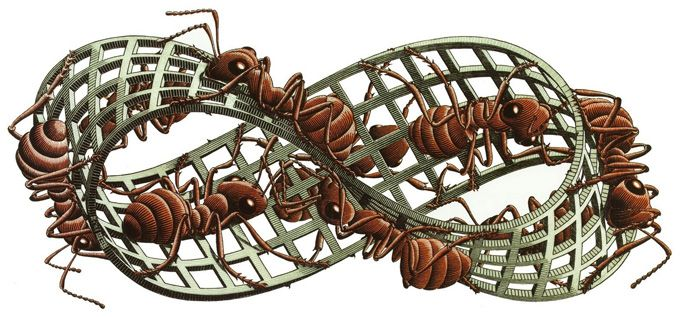
\includegraphics[width=\linewidth]{images/EscherMobius.jpg}
\end{image}%
\tcblower
\end{figureptx}%
The fact that the Möbius strip only has one boundary circle has the following surprising consequence, that makes a great "party trick", is to make a Möbius strip by taping up a strip of paper, and the cut it down the very middle of the strip -{}-{} you wind up not getting two pieces of paper, but just one!%
\par
To actually represent graphs drawn on the Möbius strip, we work similarly to what we did for the torus; we draw a square, and then we draw arrows on the left and right edges to indicate that these edges are drawn together.  However, we have one arrow drawn up, and one arrow drawn down, to indicate that the ends of the strip are glued together with a half twist.   Since the top and bottom of the Möbius strip do not get identified together at all, we do not draw any arrows on them.  Then, if an edge goes off one end the Möbius strip near the top, it comes back on the opposite end near the bottom, and vice versa.%
\begin{figureptx}{Two drawings of \(K_{3,3}\) on the Möbius strip}{x:figure:fig-K33-mobius}{}%
\begin{image}{0}{1}{0}%
\resizebox{\linewidth}{!}{%
\begin{tikzpicture}

\draw[dashed,  
        decoration={markings, mark=at position 0.55 with {\arrow[scale=4]{latex}}},     postaction={decorate}
        ] (0,0)--(6,0);
\draw[dashed,        decoration={markings, mark=at position 0.55 with {\arrow[scale=4]{latex}}},     postaction={decorate}] (0,7)--(6,7);
\draw  (0,0)--(0,7);
\draw  (6,0)--(6,7);

\node[draw, rectangle, red] (a) at (3,1) {$a$};
\node[draw, circle, blue] (x) at (4,2.5) {$x$};
\node[draw, rectangle, red] (b) at (4,4.5) {$b$};
\node[draw, circle, blue] (y) at (3,6) {$y$};
\node[draw, rectangle, red] (c) at (2,4.5) {$c$};
\node[draw, circle, blue] (z) at (2,2.5) {$z$};



\draw (a)--(x)--(b)--(y)--(c)--(z)--(a)--(y);
\draw (x)--(4,0);
\draw (b)--(4,7);
\draw (c)--(2,7);
\draw (z)--(2,0);

\node at (2, -.3) {1};
\node at (4,-.3) {2};
\node at (2,7.3) {2};
\node at (4,7.3) {1};

\begin{scope}[xshift=8cm]
\draw[dashed,  
        decoration={markings, mark=at position 0.55 with {\arrow[scale=4]{latex}}},     postaction={decorate}
        ] (0,0)--(6,0);
\draw[dashed,        decoration={markings, mark=at position 0.55 with {\arrow[scale=4]{latex}}},     postaction={decorate}] (0,7)--(6,7);
\draw  (0,0)--(0,7);
\draw  (6,0)--(6,7);

\node[draw, rectangle, red] (a) at (3,1) {$a$};
\node[draw, circle, blue] (x) at (3,2) {$x$};
\node[draw, rectangle, red] (b) at (3,3) {$b$};
\node[draw, circle, blue] (y) at (3,4) {$y$};
\node[draw, rectangle, red] (c) at (3,5) {$c$};
\node[draw, circle, blue] (z) at (3,6) {$z$};



\draw (3,0)--(a)--(x)--(b)--(y)--(c)--(z)--(3,7);

\draw (x) to [bend right] (c);
\draw (4,0) to [bend right] (a);
\draw (2,0) to [bend left] (b);
\draw (y) to [bend left] (2,7);
\draw (z) to [bend right] (4,7);

\node at (2, -.3) {1};
\node at (3, -.3) {2};
\node at (4, -.3) {3};
\node at (2, 7.3) {3};
\node at (3, 7.3) {2};
\node at (4, 7.3) {1};
\end{scope}
\end{tikzpicture}
}%
\end{image}%
\tcblower
\end{figureptx}%
Finally, we explain some heuristics about drawing graphs on surfaces, with reference drawings of \(K_{3,3}\) on the Möbius strip.  As discussed at the end of the section of the torus, it can be useful to follow part of the reasoning used in the planarity algorithm for Hamiltonian cycles when trying to draw graphs on surfaces other than the sphere.  That is, start with a large cycle in the graph -{}-{} for \(K_{3,3}\), with \(a,b,c\) red vertices, and \(x,y,z\) the blue vertices, we will use the cycle \(axbycza\).  It may be that this is cycle is drawn in the plane as a circle, as the in the left hand example; then we try to connect as many edges as possible through the centre of the circle, and then do the rest on the outside, possible wrapping around the Möbius strip.%
\par
But the Jordan Curve Theorem (that a circle has an inside and an outside) only holds for the sphere -{}-{} on other surfaces, there are always curves where this isn't true.  Whether of necessity, or choice, it might be that our large cycle is drawn as one of these loops that doesn't have an inside or an outside.  On the right hand side of \hyperref[x:figure:fig-K33-mobius]{Figure~{\xreffont\ref{x:figure:fig-K33-mobius}}}, we have drawn the cycle \(axbycz\) as the centre of the Möbius strip.%
\par
Finally, we note that in general for a surface, there are multiple different ways to draw curves; in \hyperref[x:figure:fig-K33-mobius2]{Figure~{\xreffont\ref{x:figure:fig-K33-mobius2}}}, we have drawn our chosen Hamiltonian cycle as a curve that wraps \emph{twice} about the Möbius strip.  What happens if you cut a physical Möbius strip along this line?%
\begin{figureptx}{A third drawing of \(K_{3,3}\) on the Möbius strip}{x:figure:fig-K33-mobius2}{}%
\begin{image}{0}{1}{0}%
\resizebox{\linewidth}{!}{%
\begin{tikzpicture}

\draw[dashed,  
        decoration={markings, mark=at position 0.55 with {\arrow[scale=4]{latex}}},     postaction={decorate}
        ] (0,0)--(6,0);
\draw[dashed,        decoration={markings, mark=at position 0.55 with {\arrow[scale=4]{latex}}},     postaction={decorate}] (6,7)--(0,7);
\draw  (0,0)--(0,7);
\draw  (6,0)--(6,7);

\node[draw, rectangle, red] (a) at (2,1) {$a$};
\node[draw, circle, blue] (x) at (2,3.5) {$x$};
\node[draw, rectangle, red] (b) at (2, 6) {$b$};
\node[draw, circle, blue] (y) at (4,1) {$y$};
\node[draw, rectangle, red] (c) at (4, 3.5) {$c$};
\node[draw, circle, blue] (z) at (4, 6) {$z$};

\node at (2, -.3) {1};
\node at (4,-.3) {2};
\node at (2,7.3) {2};
\node at (4,7.3) {1};

\draw (2,0)--(a)--(x)--(b)--(2,7);
\draw (4,0)--(y)--(c)--(z)--(4,7);
\draw (a)--(y);
\draw (b)--(z);
\draw (c)--(x);


\end{tikzpicture}
}%
\end{image}%
\tcblower
\end{figureptx}%
\end{subsectionptx}
\end{sectionptx}
%
%
\typeout{************************************************}
\typeout{Section 4.5 Euler's Theorem}
\typeout{************************************************}
%
\begin{sectionptx}{Euler's Theorem}{}{Euler's Theorem}{}{}{x:section:s_graphs_on_surfaces_euler}
\begin{introduction}{}%
This section cover's Euler's theorem on planar graphs and its applications. After defining faces, we state Euler's Theorem by induction, and gave several applications of the theorem itself: more proofs that \(K_{3,3}\) and \(K_5\) aren't planar, that footballs have five pentagons, and a proof that our video game designers couldn't have made their map into a sphere without doing something very strange.%
\end{introduction}%
%
%
\typeout{************************************************}
\typeout{Subsection 4.5.1 Counting faces}
\typeout{************************************************}
%
\begin{subsectionptx}{Counting faces}{}{Counting faces}{}{}{g:subsection:idp187}
A \terminology{face}\index{face} of a planar drawing of a graph is a region bounded by edges and vertices and not containing any other vertices or edges.%
\par
\hyperref[x:figure:fig_planar]{Figure~{\xreffont\ref{x:figure:fig_planar}}} shows a planar drawing of a two graphs. The left graph has determines \(5\) regions, since we also count the unbounded region that surrounds the drawing.%
\begin{figureptx}{Two planar graphs}{x:figure:fig_planar}{}%
\begin{image}{0}{1}{0}%
\resizebox{\linewidth}{!}{%
\begin{tikzpicture}


\begin{scope}[every node/.style={circle, draw, fill=red, inner sep=0pt, minimum width=4pt, thick}]

\node (a) at (0,1) {};
\node (b) at (0,2) {};
\node (c) at (1,3) {};
\node (d) at (2,2) {};
\node (e) at (2,1) {};
\node (f) at (1,0) {};

\draw (a)--(b)--(c)--(d)--(e)--(f)--(a)--(e)--(b)--(d);
\end{scope}

\begin{scope}[xshift=5cm, yshift=1.5cm, every node/.style={circle, draw, fill=red, inner sep=0pt, minimum width=4pt, thick}]

\node (a) at (0,0) {};
\node (b) at (0:2) {};
\node (c) at (120:2) {};
\node (d) at (240:2) {};

\draw (a)--(b)--(c)--(d)--(a)--(c);
\draw (b)--(d);
\end{scope}
\end{tikzpicture}
}%
\end{image}%
\tcblower
\end{figureptx}%
What happens if we compute the number of vertices minus the number of edges plus the number of faces for these drawings? We have%
\begin{align*}
6-9+5 \amp = 2\\
4-6+4 \amp =2
\end{align*}
%
\par
While it might seem like a coincidence that this computation results in \(2\) for these planar drawings, there's a more general principle at work here, and in fact it holds for \emph{any} planar drawing of \emph{any} planar graph.%
\par
In fact, the number \(2\) here actually results from a fundamental property of the plane, and there are a corresponding theorems for other surfaces. However, we only need the result as stated above.%
\begin{theorem}{Euler's Formula.}{}{g:theorem:idp188}%
\index{Euler's formula}%
Let \(\bfG\) be a connected planar graph with \(n\) vertices and \(m\) edges. Every planar drawing of \(\bfG\) has \(f\) faces, where \(f\) satisfies%
\begin{equation*}
n-m+f=2.
\end{equation*}
%
\end{theorem}
\begin{proof}{}{g:proof:idp189}
Our proof is by induction on the number \(m\) of edges. If \(m=0\), then since \(\bfG\) is connected, our graph has a single vertex, and so there is one face. Thus \(n-m+f = 1-0+1=2\) as needed. Now suppose that we have proven Euler's formula for all graphs with less than \(m\) edges and let \(\bfG\) have \(m\) edges. Pick an edge \(e\) of \(\bfG\). What happens if we form a new graph \(\bfG'\) by deleting \(e\) from \(\bfG\)? If \(\bfG'\) is connected, our inductive hypothesis applies. Say that \(\bfG'\) has \(n'\) vertices, \(m'\) edges, and \(f'\) faces. Then by induction, these numbers satisfy%
\begin{equation*}
n'-m'+f'=2.
\end{equation*}
Since we only deleted one edge, \(n'=n\) and \(m'=m-1\). What did the removal of \(e\) do to the number of faces? In \(\bfG'\) there's a new face that was formerly two faces divided by \(e\) in \(\bfG\). Thus, \(f'=f-1\). Substituting these into \(n'-m'+f'=2\), we have%
\begin{equation*}
n-(m-1)+(f-1)=2 \iff n-m+f=2.
\end{equation*}
Thus, if \(\bfG'\) is connected, we are done. If \(\bfG'\) is disconnected, however, we cannot apply the inductive assumption to \(\bfG'\) directly. Fortunately, since we removed only one edge, \(\bfG'\) has two components, which we can view as two connected graphs \(\bfG'_1\) and \(\bfG'_2\). Each of these has fewer than \(m\) edges, so we may apply the inductive hypothesis to them. For \(i=1,2\), let \(n'_i\) be the number of vertices of \(\bfG'_i\), \(m'_i\) the number of edges of \(\bfG'_i\), and \(f'_i\) the number of faces of \(\bfG'_i\). Then by induction we have%
\begin{equation*}
n'_1 - m'_1 + f'_1 = 2 \quad \text{and} \quad n'_2-m'_2+f'_2 =2.
\end{equation*}
Adding these together, we have%
\begin{equation*}
(n'_1 + n'_2) - (m'_1 + m'_2) + (f'_1 + f'_2) = 4.
\end{equation*}
But now \(n=n'_1 + n'_2\), and \(m'_1 + m'_2 = m-1\), so the equality becomes%
\begin{equation*}
n - (m-1) + (f'_1+f'_2) = 4 \iff n-m + (f'_1 + f'_2) = 3.
\end{equation*}
The only thing we have yet to figure out is how \(f'_1+f'_2\) relates to \(f\), and we have to hope that it will allow us to knock the \(3\) down to a \(2\). Every face of \(\bfG'_1\) and \(\bfG'_2\) is a face of \(\bfG\), since the fact that removing \(e\) disconnects \(\bfG\) means that \(e\) must be part of the boundary of the unbounded face. Further, the unbounded face is counted twice in the sum \(f'_1 + f'_2\), so \(f=f'_1 + f'_2 -1\). This gives exactly what we need to complete the proof.%
\end{proof}
\begin{remark}{Alternative method of dealing with the second case.}{g:remark:idp190}%
In our proof of Euler's theorem, the most complicated part was dealing with the situation if the edge \(e\) disconnects our graph \(\bfG\) when we remove it. In this case, instead of deleting the edge \(e\) we can contract it -{}-{} that is, shrink it to a point.  This would have result in a graph that is still planar and still connected, but with one less edge (\(e\) is no longer around), and one less vertex (the two vertices \(e\) connects are now merged into one).  The number of faces remains unchanged.  So the number of edges and the number of faces each decreased by one, these two changes cancel out when we calculate \(n-m+f\), and hence both are equal to two.%
\end{remark}
\end{subsectionptx}
%
%
\typeout{************************************************}
\typeout{Subsection 4.5.2 Applications of Euler's theorem}
\typeout{************************************************}
%
\begin{subsectionptx}{Applications of Euler's theorem}{}{Applications of Euler's theorem}{}{}{g:subsection:idp191}
By itself, Euler's theorem doesn't seem that useful: there are three variables (the numbers of edges, vertices, and faces) and only one equation between them, so there are still lots of degrees of freedom.  For it to be particularly useful, we want to have other relationships between these numbers.  In many applications, these relationships can come from handshaking.%
\par
Recall that Euler's handshaking lemma said that%
\begin{equation*}
\sum_{v\in G} d(v)=2 |E(G)|,
\end{equation*}
the sum of the degrees of all the vertices is twice the number of edges.  If we had some knowledge about the degrees of these vertices, we could get another relationship between the number of vertices and the number of edges.  For example, if \(G\) is regular of degree \(k\), then every vertex has degree \(k\), and hence the sum of all the degrees is just \(kn\).  Hence, handshaking would tell us that \(kn=2m\), and we would have another relationship between the three variables \(m,n\) and \(f\).%
\par
Similarly, there is a handshaking between faces and edges.  Let the \emph{degree} of a face be the number of edges that occur around it -{}-{} so, a triangle would have degree three.  Then, if we sum up the degrees of all the faces, we're counting each edge twice again -{}-{} once from the face on its left, and once from the face on its right.  so we have%
\begin{equation*}
\sum_{f\in \text{faces}(G)}d(f)=2 |E(G)|
\end{equation*}
Note that this is just the usual vertex-edge handshaking for the dual graph.%
\par
Thus, vertex-edge and face-edge handshaking can potentially give us two other sources of relationships between the numbers of vertices, edges, and faces.  Most applications of Euler's theorem proceed by combining all three relationships, as we shall see.%
\begin{lemma}{}{}{g:lemma:idp192}%
\(K_5\) isn't planar\end{lemma}
\begin{proof}{}{g:proof:idp193}
We give a proof by contradiction.  Suppose \(K_5\) was planar, and draw it on the plane.  We know that \(K_5\) has 5 vertices and \(\binom{5}{2}=10\) edges, and so by Euler theorem we know that any drawing of it must have 7 faces. We now use edge-face handshaking to get a contradiction.%
\par
What could the degrees of the faces be?  We don't know for sure, but we know that none of the faces could have degree one or two, as then the edges would form a loop or multiple edges between two vertices, but \(K_5\) is simple.  Hence, every face must have \(d(f)\geq 3\).  But then handshaking gives:%
%
\begin{equation*}
20=2e=\sum d(f)\geq \sum 3=3\cdot 7=21
\end{equation*}
which is the desired contradiction, and so we conclude that \(K_5\) is not, in fact, planar.%
\end{proof}
It is a good exercise to adapt this proof to prove that \(K_{3,3}\) isn't planar; one needs to use the extra fact that \(K_{3,3}\) doesn't have any three cycles (why not?)%
\par
We now prove that footballs have 12 pentagons.  More precisely, use the shorthand \emph{football graph} to mean any trivalent graph drawn on the plane so that every face is a pentagon or hexagon. Then we have:%
\begin{theorem}{The football theorem.}{}{g:theorem:idp194}%
Let \(\bfG\) be a football grpah drawn on the plane, with \(P\) pentagonal faces, and \(H\) hexagonal faces.  Then \(P=12\).%
\end{theorem}
\begin{proof}{}{g:proof:idp195}
Let \(V, E, F\) denote the number of vertices, edges, and faces of \(\bfG\).  Since every face is a hexagon or pentagon, we have \(E=P+H\), and substituting this into Euler's theorem gives:%
%
\begin{equation}
V-E+P+H=2\label{x:men:footeu}
\end{equation}
Now we turn handshaking.  Since \(\bfG\) is trivalent, every vertex has degree three, and so vertex-edge handshaking becomes:%
%
\begin{equation}
2E=3V\label{x:men:footve}
\end{equation}
Finally, since there are \(P\) pentagonal faces and \(H\) hexagonal faces, face-edge handshaking becomes:%
%
\begin{equation}
2E=5P+6H\label{x:men:footfe}
\end{equation}
Multiplying \hyperref[x:men:footeu]{({\xreffont\ref{x:men:footeu}})} by six gives:%
%
\begin{equation*}
6V-6E+6P+6H=12
\end{equation*}
Multiplying \hyperref[x:men:footve]{({\xreffont\ref{x:men:footve}})} by two gives \(6V-4E=0\), which we can use to eliminate \(V\), giving%
%
\begin{equation*}
-2E+5P+6H=12
\end{equation*}
Finally, using \hyperref[x:men:footfe]{({\xreffont\ref{x:men:footfe}})} we can eliminate both \(E\) and \(H\) in one go, being left with \(P=12\) as desired.%
\end{proof}
Finally, we prove that given some sensible restraints, video game designers cannot make a world map that's a sphere.  A videogame world locally looks like a square grid -{}-{} with every vertex and face having degree four.%
\begin{theorem}{The videogame theorem.}{}{g:theorem:idp196}%
It is impossible to draw for a graph to be drawn on the sphere so that every vertex and every face has degree 4.%
\end{theorem}
\begin{proof}{}{g:proof:idp197}
Since every vertex has degree 4, vertex-edge handshaking gives \(2E=4V\), and since every face has degree 4, face-edge handshaking gives \(2E=4F\).  Thus, we see \(V=F=E/2\), and plugging this in gives:%
%
\begin{equation*}
V-E+F=E/2-E+E/2=0
\end{equation*}
which contradicts Euler's Theorem.  Hence, such a graph on a sphere is not possible.%
\end{proof}
\end{subsectionptx}
\end{sectionptx}
%
%
\typeout{************************************************}
\typeout{Exercises 4.6 Exercises}
\typeout{************************************************}
%
\begin{exercises-section}{Exercises}{}{Exercises}{}{}{x:exercises:s_graphs_on_surfaces_exercises}
\begin{divisionexercise}{1}{}{}{g:exercise:idp198}%
Show that the Petersen graph has a cycle that uses all the vertices but one.  Give another proof that the Petersen graph is not planar by modifying the planarity algorithm for Hamiltonian graphs to deal with this extra vertex.\end{divisionexercise}%
\begin{divisionexercise}{2}{}{}{g:exercise:idp199}%
Draw \(K_{4,4}\) and \(K_7\) on the torus.\end{divisionexercise}%
\begin{divisionexercise}{3}{}{}{g:exercise:idp200}%
Use the planarity algorithm to show that the given graph \(\bfG\) is planar, and draw a plane graph isomorphic to it.  Explain how you might obtain a non-planar graph by adding one extra edge, and for your non-planar graph, find a subgraph that's a subdivision of \(K_5\) or \(K_{3,3}\). \begin{figureptx}{A Hamiltonian graph \(\bfG\)}{x:figure:fig-nonplanar-exercise-planarity}{}%
\begin{image}{0.15}{0.7}{0.15}%
\resizebox{\linewidth}{!}{%
\begin{tikzpicture}[scale=.7]
\tikzstyle{vertex}=[circle, draw, minimum size=17pt, inner sep=0pt]


\foreach \x in {1,2,...,9}
   \node (\x) at (40*\x:3) {\x};

\draw (8)--(1)--(2)--(3)--(4)--(5)--(6)--(7)--(8)--(9)--(1)--(3)--(6)--(4)--(2)--(5)--(7)--(9)--(3);
\draw (5)--(8)--(2);
\draw (6)--(9);




\end{tikzpicture}
}%
\end{image}%
\tcblower
\end{figureptx}%
\end{divisionexercise}%
\begin{divisionexercise}{4}{}{}{g:exercise:idp201}%
\begin{figureptx}{A Hamiltonian graph \(\bfH\)}{x:figure:fig-nonplanar-exercise-planarity2}{}%
\begin{image}{0.15}{0.7}{0.15}%
\resizebox{\linewidth}{!}{%
\begin{tikzpicture}[scale=.7]
\tikzstyle{vertex}=[circle, draw, minimum size=17pt, inner sep=0pt]


\foreach \x in {1,2,...,7}
   \node (\x) at (360/7*\x:3) {\x};

\draw (1)--(2)--(3)--(4)--(5)--(6)--(7)--(1)--(4)--(6)--(1);
\draw (3)--(7);
\draw (2)--(5);
\end{tikzpicture}
}%
\end{image}%
\tcblower
\end{figureptx}%
Let \(\bfH\) be the graph shown in \hyperref[x:figure:fig-nonplanar-exercise-planarity2]{Figure~{\xreffont\ref{x:figure:fig-nonplanar-exercise-planarity2}}}.  Show that \(\bfH\) is not planar in two ways: using the planarity algorithm, and using Kuratowski's theorem.%
\par
Draw \(\bfH\) on the Möbius strip and on a torus without the edges crossing.%
\end{divisionexercise}%
\begin{divisionexercise}{5}{}{}{g:exercise:idp202}%
A connected plane graph has faces of degrees 3 and 10 only, and every vertex has degree at least 3.  Prove that it must have fewer faces of degree 10 than of degree 3.  If every vertex has degree 3, prove that the number of faces of degree 10 must be a multiple of 3 and the number of faces of degree 3 must be a multiple of 4.%
\par
As an example, how many faces of degree 3 and degree 10 does the truncated dodecahedron possess?  (A truncated dodecahedron is obtained by sliving off each vertex of a dodecahedron to give a triangle.)%
\end{divisionexercise}%
\end{exercises-section}
\end{chapterptx}
%
%
\typeout{************************************************}
\typeout{Chapter 5 Colourings}
\typeout{************************************************}
%
\begin{chapterptx}{Colourings}{}{Colourings}{}{}{x:chapter:ch_colourings}
\begin{introduction}{}%
This chapter covers several types of colouring questions on graphs.  The initial motivation for these questions comes from an early question about colouring the countries on maps so that adjacent countries have different colours.%
\end{introduction}%
%
%
\typeout{************************************************}
\typeout{Section 5.1 Chromatic number}
\typeout{************************************************}
%
\begin{sectionptx}{Chromatic number}{}{Chromatic number}{}{}{x:section:s_chromatic_number}
The study of graph colourings began with the colouring of maps.  Usually on a map, different regions (countries, counties, states, etc.) are visually distinguished from each other by giving each one a different colour, with the idea that adjance regions should have different colours so that boundaries can be easily seen.  For instance, in this old road map of England and Wales, each county is coloured either red, yellow blue or green, and bordering counties have different colours.%
\begin{figureptx}{A historical example of a map colouring.  \href{http://www.davidrumsey.com/maps4669.html}{Image} courtesy Cartography Associates under a \href{https://creativecommons.org/licenses/by-nc-sa/2.0/}{creative commons license}}{x:figure:fig_colouredmapexample}{}%
\begin{image}{0.15}{0.7}{0.15}%
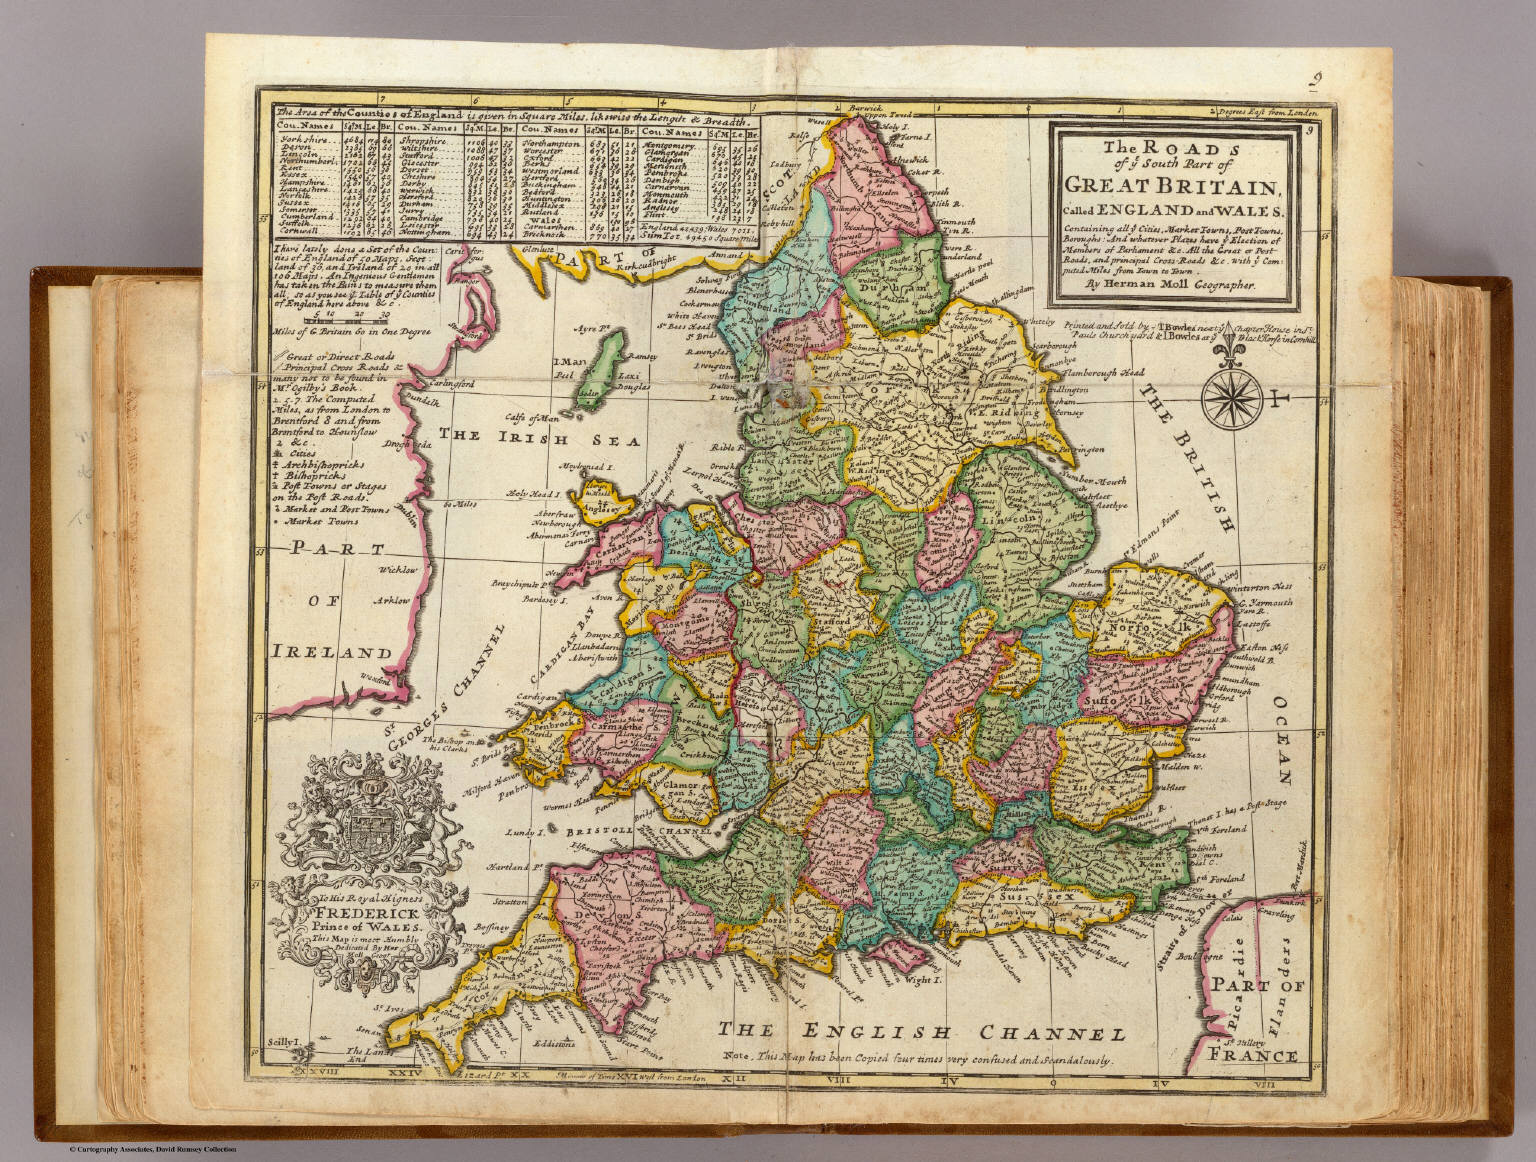
\includegraphics[width=\linewidth]{images/EnglishCounties.jpg}
\end{image}%
\tcblower
\end{figureptx}%
Note that in the map above, only four colours are used.  In 1852 Francis Guthrie suggested that for any possible map drawn on a piece of a paper, four colours would be enough.  Guthrie's conjecture wasn't proven for more than a hundred years later.%
\par
Let's make Guthrie's conjecture precise and connect it to graph theory.  Note that as in Example , it makes sense to work with essential the dual picture to the map; we make the regions of the map into vertices, and we put an edge between two regions if they share a vertex.  Then we are lead to the following definitions.%
\begin{definition}{Colourings and Chromatic number.}{g:definition:idp203}%
Let \(\bfG\) be a graph.  A \emph{\(k\)-colouring} (or sometimes \emph{vertex colouring}) of \(\bfG\) with \(k\) colours is an assignment of one of \(k\) colours to each of the vertices of \(\bfG\) so that adjacent vertices have different colours.%
\par
More formally, a \(k\)-colouring is a function \(f:V(\bfG)\to\{1,\dots,k\}\) so that if \(v\sim w\) than we have \(f(v)\neq f(w)\).%
\par
The \emph{chromatic number} of a graph \(\bfG\), written \(\chi(\bfG)\), is the least number of colours needed to colour the vertices of \(G\) so that adjacent vertices are given different colours; that is, it's the least \(k\) so that there exists a \(k\)-colouring of \(\bfG\).%
\end{definition}
The most basic problem you will have to complete about these is the following: given a graph \(\bfG\), determine its chromatic number\(\chi(\bfG)\).  Because the chromatic number is the \emph{least} number of colours with which it is possible to colour \(\bfG\), showing that \(\chi(\bfG)=N\) will always require two steps:%
%
\begin{enumerate}
\item{}Show that \(\bfG\) admits a colouring with \(\chi(\bfG)=N-1\) colours%
\item{}Show that \(\bfG\) does not admit a colouring with fewer colours.%
\end{enumerate}
\begin{example}{Complete graph.}{g:example:idp204}%
What's the chromatic number \(\chi(K_n)\) of the complete graph?  Since every vertex is adjacent to every other vertex, any two vertices need to have different colours, and so \(\chi(K_n)\geq n\).  But certainly if we colour every vertex a different colour, then two adjacent vertices have the same colour, and that's a valid colouring of \(K_n\), so \(\chi(K_n)\leq n\).   So \(\chi(K_n)=n\).%
\end{example}
\begin{example}{Trees.}{g:example:idp205}%
Suppose that \(T_n\) is a tree on \(n\geq 2\) vertices.  Then \(T_n\) has an edge, and the two vertices on this edge must be different colours, and so \(\chi(T_n)\geq 2\).  On the other hand, we can colour any tree with two colours as follows: pick any vertex, and colour it blue; then pick any vertex next to it and colour it red, then we can colour the vertices next to that blue, and colour the vertices next to those red, and continuing on outwards from our starting vertex.  Hence, \(\chi(T_n)\leq 2\) and so \(\chi(T_n)=2\).%
\par
Another way of phrasing this is that along any path we colour the vertices alternating red-blue-red-blue-red-blue.  This wouldn't work for a general graph, because there may be two paths of different lengths between a pair of vertices \(v\) and \(w\).  But in trees because there is always exactly one path between any two vertices, and so once we colour one vertex, there's a unique way to colour all the others with two colours in this way.%
\end{example}
\begin{example}{Cyclic graphs \(C_n\).}{g:example:idp206}%
As with trees, as long as \(n\geq 2\) the graph has at least one edge, and thus has \(\chi(C_n)\geq 2\).  Can we colour \(C_n\) with two colours?%
\par
If we could, the vertices would have to alternate red-blue-red-blue all the way around.  This works if \(n\) is even, but if \(n\) is odd then the vertex we started with would have the same colour as the vertex we ended with, but they're adjacent.  Thus, when \(n\) is odd we need at least three colours to colour the graph, but it's easy to do with three colours -{}-{} we can alternate red-blue-red-blue, but make the very last vertex green, for instance.%
\par
Summarizing, we have:%
\begin{equation*}
\chi(C_n)=\begin{cases} 2 & n \text{ odd} \\ 3 & n \text{ even} \end{cases}
\end{equation*}
%
\end{example}
In fact, as thinking about the examples of trees and cycles should show, we've already met one instance of the chromatic number -{}-{} a graph \(\bfG\) is bipartite if and only if \(\chi(\bfG)=2\), as follows immediately from the definition.%
\par
Another useful observation about the examples we've seen is that, since the chromatic number \(\chi(\bfG)\) is the \emph{least} number of colours needed to colour \(\chi(\bfG)\), to show that \(\chi(\bfG)=s\) requires doing two things:%
\begin{enumerate}
\item{}Showing that \(\bfG\) \emph{can} be coloured with \(s\) colours, and hence \(\bfG\leq s\)%
\item{}Showing that \(\bfG\) \emph{can't} be coloured with \(s-1\) colours, and hence \(\bfG\geq s\)%
\end{enumerate}
%
\begin{example}{The Wheel graph.}{g:example:idp207}%
The wheel graph \(W_n\) consists of an \(n\)-cycle together with one additional vertex, that is connected to all vertices of the \(n\)-cycle.  Note that this with this convention, \(W_n\) confusingly has \(n-1\) vertices; other people may use a different convention where \(W_n\) has \(n\) vertices, but then it only has a \(n-1\) vertices on the actual wheel.%
\par
Since the central vertex is connected to all other vertices, once we colour it, we can never use that colour again.  But deleting that vertex we just have the \(n\)-cycle, and we already know the chromatic number of that.  So we have \(\chi(W_n)=\chi(C_n)+1\).%
\end{example}
\begin{definition}{}{g:definition:idp208}%
We write \(\Delta(\bfG)\) for the maxium degree of any vertex in \(\bfG\):%
\begin{equation*}
\Delta(\bfG)=\max_{v\in \bfG} d(v)
\end{equation*}
%
\end{definition}
\begin{theorem}{}{}{g:theorem:idp209}%
We have \(\chi(\bfG)\leq \Delta(\bfG)+1\)%
\end{theorem}
\begin{proof}{}{g:proof:idp210}
We need to show that we can colour any graph \(\bfG\) with \(\Delta(G)+1\) colours.  But we can just colour the vertices of \(\bfG\) one by one in whatever order we want.  When we go to colour the \(i\)th vertex \(v_i\), we look at the \(d(v_i)\) vertices adjacent to \(v_i\).  Some of them may not be coloured yet, in which case they don't affect anything, but for each vertex adjacent to \(v_i\) that is coloured, we can't use that colour for \(v_i\).%
\par
So there are most \(d(v_i)\leq \Delta(\bfG)\) colours we have to avoid; if we have \(\Delta(\bfG)+1\) colours to choose from we can always find one that hasn't been used at a vertex adjacent to \(v_i\)%
.\end{proof}
\end{sectionptx}
%
%
\typeout{************************************************}
\typeout{Section 5.2 Chromatic index and applications}
\typeout{************************************************}
%
\begin{sectionptx}{Chromatic index and applications}{}{Chromatic index and applications}{}{}{x:section:s_chromatic_index}
It is a natural twist of the definition of chromatic number to try to colour the edges of a graph instead; the least number of colours needed is the called the \emph{chromatic index}.  After introducing this concept and giving some examples, we give some story problem type questions that boil down to finding either the chromatic number or chromatic index.%
\begin{definition}{Chromatic index.}{g:definition:idp211}%
The \emph{chromatic index} \(\chi^\prime(\bfG)\) of a graph \(\bfG\) is the least number of colours needed to colour the edges of \(\bfG\) so that any two edges that share a vertex have different colours.%
\end{definition}
Not that as with the chromatic number, since the chromatic index \(\chi^\prime(\bfG)\) is the minimum number of colours such that the edges can be coloured with adjacent edges having different colours, to show \(\chi^\prime(\bfG)=N\) typically requires two steps:%
%
\begin{enumerate}
\item{}Prove that the edges of \(\bfG\) can be coloured with \(N\) colours%
\item{}Prove that the edges of \(\bfG\) cannot be coloured with less than \(N\) colours%
\end{enumerate}
\begin{example}{The complete graph \(K_4\).}{g:example:idp212}%
Let's find \(\chi^\prime(K_4)\).  Picking any vertex \(v\), there are three edges incident to \(v\), and none of these edges can have the same colour (as they all meet at \(v\)).  Hence, we have \(\chi^\prime(K_4)\geq 3\).%
\par
On the other hand, it is easy to colour the edges of \(K_4\) with three colours, as seen below, and so \(\chi^\prime(K_4)\leq 3\), and hence \(\chi^\prime(K_4)=3\).%
\end{example}
\begin{example}{The complete graph \(K_5\).}{g:example:idp213}%
Now, let's move on to \(K_5\).  Again, looking at any vertex we see all the edges adjacent to that vertex must be different colours, and so we have \(\chi^\prime(K_5)\geq 4\).   Let's try to colour the edges of \(K_5\) with 4 colours.%
\begin{sidebyside}{2}{0.025}{0.025}{0.05}%
\begin{sbspanel}{0.6}[center]%
Suppose we coloured the four edges adjacent to the top vertex blue, green, red and purple, from left to right, and now look at the bottom edge.  It is adjacent to edges coloured green and red, and so must be blue or purple.  By symmetry, it's equivalent to colour it either colour, so let's suppose it's blue, giving us the following picture:%
\end{sbspanel}%
\begin{sbspanel}{0.3}[center]%
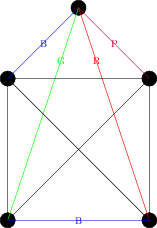
\includegraphics[width=\linewidth]{images/K5EdgeColouring1.png}
\end{sbspanel}%
\end{sidebyside}%
\begin{sidebyside}{2}{0.025}{0.025}{0.05}%
\begin{sbspanel}{0.6}[center]%
Now the edge on the right is adjacent to edges coloured red, blue and purple, and so must be green.  But now we have a problem -{}-{} consider the edges labeled \(x\) and \(y\) in the next drawing:%
\end{sbspanel}%
\begin{sbspanel}{0.3}[center]%
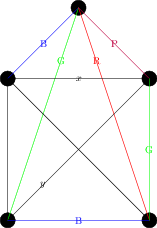
\includegraphics[width=\linewidth]{images/K5EdgeColouring2.png}
\end{sbspanel}%
\end{sidebyside}%
Both edges share vertices with edges coloured green, blue, and purple, and hence each would need to be coloured red.  But they also share a vertex with each other, and so cannot both be coloured red.  So we see \(\chi^\prime(K_5)\geq 5\).%
\begin{sidebyside}{2}{0.025}{0.025}{0.05}%
\begin{sbspanel}{0.6}[center]%
On the other hand, it is easy to colour the edges of \(K_5\) with 5 colours:  colour each edge in the outside pentagon a different colour.  For each edge in the outside pentagon there will be a unique edge in the inside star that does meet that edge (the one "parallel" to it) -{}-{} draw that edge the same colour.  That results in the following colouring:%
\end{sbspanel}%
\begin{sbspanel}{0.3}[center]%
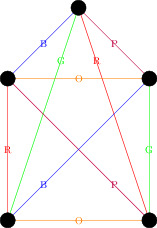
\includegraphics[width=\linewidth]{images/K5EdgeColouring3.png}
\end{sbspanel}%
\end{sidebyside}%
\end{example}
In the examples above, we found lower bounds for \(\chi^\prime(\bfG)\) by considering the degrees of vertices; this argument easily adapts in general.%
\begin{theorem}{}{}{g:theorem:idp214}%
For any graph \(\bfG\) we have \(\chi^\prime(\bfG)\geq\Delta(\bfG)\)%
\end{theorem}
\begin{proof}{}{g:proof:idp215}
Let \(v\in\bfG\) be a vertex of maximal degree \(d(v)=\Delta(\bfG)\).  Then none of the \(\Delta(\bfG)\) edges incident to \(v\) can be coloured the same colour, and so we have \(\chi^\prime(\bfG)\geq \Delta(\bfG)\)%
\end{proof}
It turns out that this nearly determines the chromatic index \(\chi^\prime(\bfG)\) -{}-{} it can be at most one more than \(\Delta(\bfG)\):%
\begin{theorem}{Vizing's Theorem.}{}{g:theorem:idp216}%
For any graph \(\bfG\) we have \(\Delta(\bfG)\leq \chi^\prime(\bfG)\leq \Delta(\bfG)+1\)%
\end{theorem}
\begin{proof}{}{g:proof:idp217}
The lower bound was just proved in the previous theorem.  The other direction is more difficult.%
\end{proof}
We now show how determining the chromatic number and chromatic index can show up as part of story questions.%
\par
Suppose there are six friends, Alice, Bob, Charlie, Dora, Elizabeth and Frank, and there is the following graph between then:%
\begin{sidebyside}{2}{0.025}{0.025}{0.05}%
\begin{sbspanel}{0.5}[center]%
\resizebox{\linewidth}{!}{%
{\centering%
{\tabularfont%
\begin{tabular}{c}
A\tabularnewline\hrulemedium
\multicolumn{1}{cB}{X}&B\tabularnewline\hrulemedium
\multicolumn{1}{cB}{X}&\multicolumn{1}{cB}{}&C\tabularnewline\hrulemedium
\multicolumn{1}{cB}{}&\multicolumn{1}{cB}{X}&\multicolumn{1}{cB}{X}&D\tabularnewline\hrulemedium
\multicolumn{1}{cB}{X}&\multicolumn{1}{cB}{}&\multicolumn{1}{cB}{X}&\multicolumn{1}{cB}{}&E\tabularnewline\hrulemedium
\multicolumn{1}{cB}{}&\multicolumn{1}{cB}{X}&\multicolumn{1}{cB}{}&\multicolumn{1}{cB}{X}&\multicolumn{1}{cB}{X}&F
\end{tabular}
}%
\par}
}%
\end{sbspanel}%
\begin{sbspanel}{0.4}[center]%
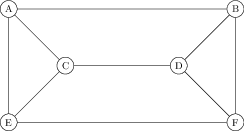
\includegraphics[width=\linewidth]{images/ChromaticNumberVsIndex.png}
\end{sbspanel}%
\end{sidebyside}%
Here are two word problems related to \(\bfG\):%
%
\begin{enumerate}
\item{}The friends want to divide into groups, but the edges indicate people who currently annoy each other.  What's the least number of groups the friends can divide into groups so that no group contains two people who annoy each other?%
\item{}The friends want to hold a snooker tournament, with everyone playing three matches; the edges indicate pairs of friends who will play against each other.  If multiple matches can be played each day, but each person can only be involved in one match a day, how many days are necessary to hold the tournament?%
\end{enumerate}
The first case concerns the chromatic number -{}-{} each group of people will be the people who have the same colour, and we don't want vertices with an edge between them to have the same colour.%
\par
The second case concerns the chromatic index -{}-{} the edges are the games that are being played, and all edges that are the same colour will be played on the same day.%
\par
Let us quickly compute the chromatic number and chromatic index of the graph \(\bfG\) above.  To compute the chromatic number, we observe that the graph contains a triangle, and so the chromatic number is at least 3.  But it is easy to colour the vertices with three colours -{}-{} for instance, colour A and D red, colour C and F blue, and colur E and B green.  So \(\chi(\bfG)=3\).%
\par
To compute \(\chi^\prime(G)\), since \(A\) has degree three we have \(\chi^\prime(\bfG)\geq 3\).  On the other hand, it is easy to colour the edges with three colours -{}-{} for instance, colour AB, CE and DF red, colour AE, CD and BF blue, and colour AC, BD and EF green.  So \(\chi^\prime(\bfG)=3\) as well.%
\end{sectionptx}
%
%
\typeout{************************************************}
\typeout{Section 5.3 Introduction to the chromatic polynomial}
\typeout{************************************************}
%
\begin{sectionptx}{Introduction to the chromatic polynomial}{}{Introduction to the chromatic polynomial}{}{}{x:section:s_chromatic_polynomial_intro}
\begin{introduction}{}%
For the chromatic number, we were asking whether or not it was possible to colour the vertices of \(\bfG\) with a given number of colours.  The chromatic polynomial extends this question, and asks the following.  Suppose we have \(k\) colours.  How many different ways can we colour the vertices of \(\bfG\)?  It is \emph{not} clear that this should be a polynomial in \(k\), and proving that it is in fact a polynomial in \(k\) is the highlight of the section.%
\end{introduction}%
%
%
\typeout{************************************************}
\typeout{Subsection 5.3.1 Definition and examples}
\typeout{************************************************}
%
\begin{subsectionptx}{Definition and examples}{}{Definition and examples}{}{}{g:subsection:idp218}
\begin{definition}{The chromatic polynomial \(P_{\bfG}\).}{g:definition:idp219}%
The chromatic polynomial \(P_{\bfG}\) of a graph \(\bfG\) is the function that takes in a non-negative integer \(k\) and returns the number of ways to colour the vertices of \(\bfG\) with \(k\) colours so that adjacent vertices have different colours.%
\end{definition}
It is immediate from the definition of the chromatic polynomial that \(\chi(\bfG)\) is the least positive number \(k\) such that \(\chi_{\bfG}(k)\neq 0\).%
\par
It is \(not\) immediate from the definition of the chromatic polynomial that it is, in fact, a polynomial.  In fact, proving that will take a little bit of work, and we postpone this until the end.  First, we look at some examples of the chromatic polynomial; in many cases it is possible to easily compute the chromatic polynomial by working "vertex by vertex".%
\begin{example}{The empty graph \(E_n\).}{g:example:idp220}%
Recall that the empty graph \(E_n\) has \(n\) vertices and no edges.  To compute \(P_{E_n}(k)\) we need to count the number of ways to colour the vertices with \(k\) colours.  But since \(E_n\) has no edges, we can colour each of the \(n\) vertices any of the \(k\) colours; the choices are completely independent.  So \(P_{E_n}(k)=k^n\)%
\end{example}
\begin{example}{The complete graph \(K_n\).}{g:example:idp221}%
Let's label the vertices \(v_0,\dots, v_{n-1}\), and colour them one by one in the given order.  When we colour the first vertex \(v_0\), no other vertices have been coloured, and we can use whichever of the \(k\) vertice we like.  However, when we go to colour \(v_1\) we note that it is adjacent to \(v_0\), and so whatever colour we used for \(v_0\) we can't for \(v_1\), and so we have \(k-1\) colours to choose for \(v_1\)%
\par
Continuing in this way, we see that since all the vertices are adjacent, they all most have different colours.  So when we go to colour \(v_i\), we have already coloured \(v_o,\dots, v_{i-1}\) with \(i\) different colours, and we can't use any of these to colour \(v_i\), and so we have \(k-i\) choices to colour \(v_i\).%
\par
Putting it all together, we see that:%
\begin{equation*}
P_{K_n}(k)=k\cdot (k-1)\cdot (k-2)\cdots k-n+1
\end{equation*}
%
\end{example}
\begin{example}{Two triangles joined at a vertex.}{x:example:example_bowtie_chromatic_polynomial}%
\begin{sidebyside}{2}{0.025}{0.025}{0.05}%
\begin{sbspanel}{0.6}%
Consider the graph \(\bfG\) consisting of two triangles joined at the right a vertex, shown at the right.  We can calulate \(P_\bfG(k)\) by working vertex by vertex: there are \(k\) ways to colour vertex 1, but then when we colour vertex 2 it can't be the same as vertex 1, and so there are \(k-1\) ways to colour it.  Vertex three is adjacent to both one and two, so there are \(k-2\) ways to colour it, and vertex 4 is adjacent to one coloured vertex, vertex 3, so there are again \(k-1\) ways to colour it, and finally vertex 5 is adjacent to vertices 3 and 4 and so we have \(k-2\) ways to colour it.Putting it together, we see \(P_\bfG(k)=k(k-1)^2(k-2)^2\).%
\end{sbspanel}%
\begin{sbspanel}{0.3}%
\resizebox{\linewidth}{!}{%
\begin{tikzpicture}[scale=2]
\tikzstyle{vertex}=[circle, draw, minimum size=17pt, inner sep=0pt]
\node[vertex] (V1) at (0,0) {$1$};
\node[vertex] (V2) at (0,2) {$2$};
\node[vertex] (V3) at (1,1) {$3$};
\node[vertex] (V4) at (2,0) {$4$};
\node[vertex] (V5) at (2,2) {$5$};
\path  (V1) edge (V2)
(V4) edge (V5)
(V3) edge (V1)
     edge (V2)
     edge (V4)
     edge (V5);

\end{tikzpicture}
}%
\end{sbspanel}%
\end{sidebyside}%
\end{example}
\begin{example}{Two triangles joined along an edge.}{g:example:idp222}%
\begin{sidebyside}{2}{0.025}{0.025}{0.05}%
\begin{sbspanel}{0.6}%
Consider the graph \(H\) consisting of two triangles joined along an edge. shown at the right.  We can calulate \(P_H(k)\) by working vertex by vertex: there are \(k\) ways to colour vertex 1, but then when we colour vertex 2 it can't be the same as vertex 1, and so there are \(k-1\) ways to colour it.  Vertex three is adjacent to both one and two, so there are \(k-2\) ways to colour it, and vertex 4 is adjacent to vertices 2 and 3, which have different colours as they are adjacent to each other, so there are \(k-2\) ways to colour it.  Putting it together, we see \(P_H(k)=k(k-1)(k-2)^2\)%
\end{sbspanel}%
\begin{sbspanel}{0.3}%
\resizebox{\linewidth}{!}{%
\begin{tikzpicture}[scale=2]
\tikzstyle{vertex}=[circle, draw, minimum size=17pt, inner sep=0pt, rotate=90]
\node[vertex] (V1) at (0,1) {$1$};
\node[vertex] (V2) at (2,0) {$2$};
\node[vertex] (V3) at (2,2) {$3$};
\node[vertex] (V4) at (4,1) {$4$};
\path  (V1) edge (V2)
            edge (V3)
       (V2) edge (V3)
            edge (V4)
       (V3) edge (V4);

\end{tikzpicture}
}%
\end{sbspanel}%
\end{sidebyside}%
\end{example}
\end{subsectionptx}
%
%
\typeout{************************************************}
\typeout{Subsection 5.3.2 Gluing}
\typeout{************************************************}
%
\begin{subsectionptx}{Gluing}{}{Gluing}{}{}{g:subsection:idp223}
What can we say about the chromatic polynomial of a graph \(\bfG\) that's the disjoint union of two smaller graphs: \(\bfG=\bfG_1\sqcup \bfG_2\)?%
\par
We already covered the extreme case where \(\bfG=E_n\) is just a disjoint union of vertices; we could colour each vertex independently of the others, as there were no edges between them at all. A similar argument works in general to give the following.%
\begin{proposition}{}{}{g:proposition:idp224}%
Let \(\bfG=\bfG_1\sqcup \bfG_2\) be a disconnected graph.  Then \(P_{\bfG}(k)=P_{\bfG_1}(k)P_{\bfG_2}(k)\)%
\end{proposition}
\begin{proof}{}{g:proof:idp225}
A colouring of \(\bfG\) with \(k\) colours gives a colouring of \(\bfG_1\) with \(k\) colours and a colouring of \(\bfG_2\) with \(k\) colourings. Similarly, since \(\bfG_1, \bfG_2\) are disconnected, how we colour one will have no effect on what colourings are possible for the other.  Hence, colouring \(\bfG\) is exactly the same as colouring \(\bfG_1\) and \(\bfG_2\)%
\end{proof}
 It gets more interesting if \(\bfG\) is \emph{almost} the disjoint union of two graphs, by which we mean that \(\bfG\) is the union of two subgraphs \(\bfG_1\) and \(\bfG_2\) that are nearly disjoint -{}-{} perhaps they share a single vertex, or two vertices connected by an edge.  In these cases, there are nice "gluing" formulas relating the chromatic polynomials of \(\bfG, \bfG_1\) and \(\bfG_2\); as \(\bfG_1\cap\bfG_2\) grows more complicated it is still possible to say something but the answer gets more complicated and not worth it. \begin{proposition}{}{}{g:proposition:idp226}%
Suppose \(\bfG\) has two subgraphs \(\bfG_1\) and \(\bfG_2\), so that their union is all of \(\bfG\), but their intersection is a single vertex \(v\), i.e. \(\bfG_1\cup\bfG_2=\bfG\) and \(\bfG_1\cap\bfG_2=\{v\}\).  Then we have the following relation between their chromatic polynomials:%
%
\begin{equation*}
P_{\bfG}(k)=\frac{1}{k}P_{\bfG_1}(k)P_{\bfG_2}(k)
\end{equation*}
\end{proposition}
\begin{proof}{}{g:proof:idp227}
As in the proof of colourings of disjoint unions, a colouring of \(\bfG\) gives a colouring of both \(\bfG_1\) and \(\bfG_2\) by restriction, but we don't get any two colourings: both \(\bfG_1\) and \(\bfG_2\) contain \(v\), and our two colourings must both make \(v\) the same colouring.%
\par
In the other direction, if we have colourings of \(\bfG_1\) and \(\bfG_2\) that have the same colour at \(v\), it is clear that we can glue them together to get a colouring of \(\bfG\).  So the question reduces to the following: given that we want vertex \(v\) to have a fixed colour, how many colourings of \(\bfG_2\) are there that colour \(v\) this colour?%
\par
The \(k\) colours are completely interchangeable, however; we could just change the names of each one.  Thus, it is clear that there are as many colourings of \(\bfG_2\) where \(v\) is red as there are where \(v\) is blue as there are where \(v\) is any given colour.  Hence, if we have \(k\) colours to use, exactly \(1/k\) of all colourings of \(\bfG_2\) will ahve \(v\) any given colour, namely \(P_{\bfG_2}(k)/k\)%
\par
Thus, to colour \(\bfG\) with \(k\) colours, we first could first colour \(\bfG_1\) in one of the \(P_{\bfG_1}(k)\) ways.  This will give us a some fixed colour of \(v\), and we saw above that there are \(P_{\bfG_2}(k)/k\) colourings of \(\bfG_2\) where \(v\) has this colour, and so we have the result.%
\end{proof}
\begin{example}{Two triangles joined at a vertex, again.}{g:example:idp228}%
As an example, we revisit our previous example.  For \(\bfG\), two triangles joined at a vertex, we have \(\bfG_1\cong \bfG_2\cong C_3\).  Since \(C_3\cong K_3\), we know \(P_{C_3}(k)=k(k-1)(k-2)\).  Thus, we have:%
%
\begin{equation*}
P_\bfG(k)=\frac{P_{C_3}(k)P_{C_3}(k)}{k}=\frac{k^2(k-1)^2(k-2)^2}{k}=k(k-1)^2(k-2)^2
\end{equation*}
\end{example}
\begin{proposition}{}{}{g:proposition:idp229}%
Suppose \(\bfG\) has two subgraphs \(\bfG_1\) and \(\bfG_2\), so that their union is all of \(\bfG\), but their intersection is a single vertex edge \(e\) connecting two vertices \(v\) and \(u\), i.e. \(\bfG_1\cup\bfG_2=\bfG\) and \(\bfG_1\cap\bfG_2=\{e\}\).  Then we have the following relation between their chromatic polynomials:%
%
\begin{equation*}
P_{\bfG}(k)=\frac{1}{k(k-1)}P_{\bfG_1}(k)P_{\bfG_2}(k)
\end{equation*}
\end{proposition}
\begin{proof}{}{g:proof:idp230}
The proof is extremely similar to that of the previous proposition.  A colouring of \(\bfG\) gives us colourings of \(\bfG_1\) and \(\bfG_2\), but not any two colourings: they need to match at both \(v\) and at \(u\).%
\par
Now, \(v\) could be any of the \(k\) colours, but \(u\), being adjacent to \(v\), can't be the same colour, and so it has \(k-1\) possibilities given a choose of colour for \(v\).  Thus, there are \(k(k-1)\) ways to colour \(v\) and \(u\), and all possibilities will occur equally often within the colourings counted by \(P_{\bfG_2}(k)\).  Hence, given a colouring of \(\bfG_1\), there will be \(P_{\bfG_2}(k)/[k(k-1)]\) ways to extendthat colouring to one of all of \(G\), giving us the result.%
\end{proof}
\begin{example}{Two triangles joined along an edge, again.}{g:example:idp231}%
As an example, we revisit our previous example.  For \(H\), two triangles joined along an edge, we can apply the theorm with \(\bfG_1\cong \bfG_2\cong C_3\).  Thus, we have:%
%
\begin{equation*}
P_H(k)=\frac{P_{C_3}(k)P_{C_3}(k)}{k(k-1)}=\frac{k^2(k-1)^2(k-2)^2}{k}=k(k-1)(k-2)^2
\end{equation*}
\end{example}
\end{subsectionptx}
%
%
\typeout{************************************************}
\typeout{Subsection 5.3.3 Case by case analysis}
\typeout{************************************************}
%
\begin{subsectionptx}{Case by case analysis}{}{Case by case analysis}{}{}{g:subsection:idp232}
The meethods of gluing and working vertex by vertex make many chromatic polynomials easy to calculate.  Other graphs, however, are not amenable to our gluing theorems, and require considering several cases when working vertex by vertex.%
\begin{example}{The chromatic polynomial of the cycle \(C_4\).}{g:example:idp233}%
\begin{sidebyside}{2}{0.025}{0.025}{0.05}%
\begin{sbspanel}{0.6}%
Now consider the graph \(C_4\), shown at right, and suppose we try to count the number of colourings of it with \(k\) colours.  Vertex 1 can be any of \(k\) colours, and vertex 2 has \(k-1\) possibilities -{}-{} any colour except the one used for vertex 1.  Moving to vertex 4, we see it is just adjacent to 1 as well, and so has \(k-1\) possibilities as well.%
\end{sbspanel}%
\begin{sbspanel}{0.3}%
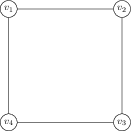
\includegraphics[width=\linewidth]{images/c4.png}
\end{sbspanel}%
\end{sidebyside}%
It becomes more difficult when we try to colour vertex 3.  It is adjacent to vertices 2 and 4, and so cannot be the same colour as either of these.  However, vertices 2 and 4 are not adjacent, and so we don't know whether they have the same colour or not.  If vertices 2 and 4, have the same colour there are \(k-1\) possibilities for vertex 3, while if vertices 2 and 4 have different colours, there are only \(k-2\) possibilties.  Thus, we must count how many possibilities are in each of these cases.%
\par
If we want vertices 2 and 4 to have the same colour, we can first colour vertex 1 in \(k\) different ways, and then pick any of the remaining \(k-1\) colours for vertices 2 and 4.  Then, to complete this to a colouring of \(C_4\), we have to colour \(v_3\), which can be any of the \(k-1\) colours that aren't the colour \(v_2\) and \(v_4\) are coloured.  Thus, the case where \(v_2\) and \(v_4\) have the same colour has \(k(k-1)^2\) possibilities.%
\par
If we want vertices 2 and 4 to have different colours, then we can first colour \(v_1\) any of \(k\) colours, colour \(v_2\) any of \(k-1\) colours.  Now, when we go to colour vertex 4 it can't be the same colour as vertex 1 since they are adjacent, and it can't be the same colour as vertex 2 by our supposition.  Vertices \(v_1\) and \(v_2\) have different colours, and so this leaves \(k-2\) possibilities for \(v_4\).  Thus there are \(k(k-1)(k-2)\) possibilities to colour vertices 1, 2 and 4 so that 2 and 4 have different colours, and then there are \(k-2\) possibilities left for vertex 3, giving \(k(k-1)(k-2)^2\) ways to colour \(C_4\) so that vertices 2 and 4 have different colours.%
\par
Adding the two cases together, this gives:%
%
\begin{align*}
P_{C_4}(k)\amp=k(k-1)^2+k(k-1)(k-2)^2\\
\amp=k(k-1)[k-1+(k-2)^2]\\
\amp=k(k-1)(k^2-3k+3)
\end{align*}
\end{example}
\begin{example}{The chromatic polynomial of \(C_5\).}{g:example:idp234}%
\begin{sidebyside}{2}{0.025}{0.025}{0.05}%
\begin{sbspanel}{0.6}%
A similar case-by-case argument that we made for \(C_4\) works for \(C_5\), except now we have a further case to deal with.  Using the vertex labellings as shown to the right, note that Vertices 3 and 4 must have different colours.  We will consider three cases: Vertices 1, 3 and 4 all have different colours, Vertex 1 has the same colour as Vertex 3, and Vertex 1 has the same colour as Vertex 4.%
\end{sbspanel}%
\begin{sbspanel}{0.3}%
\resizebox{\linewidth}{!}{%
\begin{tikzpicture}[scale=2]
\tikzstyle{vertex}=[circle, draw, minimum size=17pt, inner sep=0pt]
\node[vertex] (1) at (90:2cm) {$1$};
\node[vertex] (2) at (18:2cm) {$2$};
\node[vertex] (3) at (-54:2cm) {$3$};
\node[vertex] (4) at (234:2cm) {$4$};
\node[vertex] (5) at (162:2cm) {$5$};
\draw (1)--(2)--(3)--(4)--(5)--(1);
\end{tikzpicture}
}%
\end{sbspanel}%
\end{sidebyside}%
Case 1: 1, 3 and 4 have different colours.  Then there are \(k(k-1)(k-2)\) ways to colour vertices 1, 3, and 4, since they must all be different colours.  When we go to colour vertices 2 and 5, we see that they are each adjacent to two vertices known to have different colours, and so there are \(k-2\) ways to colour each of them.  Thus in total, Case 1 contains \(k(k-1)(k-2)^3\) colourings.%
\par
Case 2: 1 and 3 have the same colour. Then there are \(k\) ways to choose this colour, and \(k-1\) ways to choose a colour for vertex 2 (since 1 and 3 have the same colour), and \(k-1\) ways to choose a colour for vertex 4.  When we colour vertex 5, we know that 1 and 4 must have different colours, and so we have \(k-2\) ways to colour vertex 5.  Thus in total, Case 2 contains \(k(k-1)^2(k-2)\) colourings.%
\par
By symmetry, we see that Case 3, where 1 and 4 have the same colour, is identical to Case 2.  Thus, putting the three cases together, we see that:%
%
\begin{align*}
P_{C_5}(k)\amp=k(k-1)(k-2)^3+2k(k-1)^2(k-2)\\
\amp=k(k-1)(k-2)[(k-2)^2+2(k-1)]\\
\amp=k(k-1)(k-2)(k^2-2k+2)
\end{align*}
\end{example}
\end{subsectionptx}
\end{sectionptx}
%
%
\typeout{************************************************}
\typeout{Section 5.4 Chromatic Polynomial continued}
\typeout{************************************************}
%
\begin{sectionptx}{Chromatic Polynomial continued}{}{Chromatic Polynomial continued}{}{}{x:section:s_chromatic_polynomial_more}
\begin{introduction}{}%
It may seem plausible that, if we consider enough cases, the case-by-case method of computing the chromatic polynomial would work for any graph, no matter how complicated.  Assuming this, it would follow that the chromatic polynomial \(P_\bfG(k)\) is in fact a polynomial.  However, plausibility does not make a proof.  In this section we complete the proof elegantly using induction, but first need to introduce the notion of deletion and contraction.%
\end{introduction}%
%
%
\typeout{************************************************}
\typeout{Subsection 5.4.1 Deletion-Contraction}
\typeout{************************************************}
%
\begin{subsectionptx}{Deletion-Contraction}{}{Deletion-Contraction}{}{}{g:subsection:idp235}
\begin{definition}{Deletion.}{g:definition:idp236}%
Let \(\bfG\) be a graph, and let \(e\in\bfG\) be a graph.  Then we use \(\bfG\setminus e\) to denote the graph with the same vertex set as \(\bfG\), and with all the same edges, except the edge \(e\) deleted.%
\end{definition}
\begin{definition}{Contraction.}{x:definition:def-contract}%
Let \(\bfG\) be a simple graph, and let \(e\in \bfG\) be an edge between vertices \(v\) and \(w\).  Then \(\bfG/e\), the graph with \(e\) contracted.  More precisely, \(\bfG/e\) is the simple graph with vertices \(V(\bfG/e)=V(\bfG)\setminus \{v,w\}\cup {e}\).  Two non-\(e\) vertices are adjacent in \(\bfG/e\) if and only if they were adjacent in \(\bfG\), and a vertex \(y\) is adjacent to \(e\) in \(\bfG\) if and only if it was adjacent to \(v\) or \(w\) in \(\bfG\).%
\end{definition}
Formally, \hyperref[x:definition:def-contract]{Definition~{\xreffont\ref{x:definition:def-contract}}} seems formidable, but intuitively it is not as bad as the definition looks: we are changing \(\bfG\) by making the whole edge \(e\) into one vertex.  This may create multiple edges if a vertex was adjacent to both \(v\) and \(w\), and if so we simply remove any duplicate edges.%
\begin{lemma}{Deletion-Contraction.}{}{x:lemma:lem-deletion-contraction}%
Let \(\bfG\) be a simle graph, and let \(e\in \bfG\) be any edge.  Then we have:%
%
\begin{equation*}
P_\bfG(k)=P_{\bfG\setminus e}(k)-P_{\bfG/e}(k)
\end{equation*}
\end{lemma}
\begin{proof}{}{g:proof:idp237}
Since \(\bfG\) and \(\bfG\setminus e\) have the same vertex, it is not too difficult to compare their colourings.  Any valid colouring of \(\bfG\) will give a colouring of \(\bfG\setminus e\), but not every colouring of \(\bfG\setminus e\) arises this way -{}-{} in \(\bfG\), colourings require that \(v\) and \(w\), the two endpoints of \(e\), have different colours, but there is no such requirement for \(\bfG\setminus e\).  So, we want to count the colourings of \(\bfG\setminus e\) where \(v,w\) have the same colour.  But these are just the colourings of \(\bfG/e\): given a colouring of \(\bfG/e\)m we can get a colouring of \(\bfG\) by giving most vertices the same colour, and giving both \(v,w\) whatever colour \(e\) was.  By definition, we see that \(v\) and \(w\) will have the same colour in this colouring; and given any colouring of \(\bfG\setminus e\) where \(v,w\) have the same colour we can get a colouring of \(\bfG/e\) by colouring \(e\) the colour that \(v,w\) were.%
\end{proof}
\begin{example}{Chromatic polynomial of \(C_4\), again.}{g:example:idp238}%
Let us compute \(P_{C_4}(k)\) a different way as an illustration of how deletion-contraction works.  No matter which edge of \(C_4\) we pick, \(C_4\setminus e\) will be the path graph \(P_4\), which is a tree, and hence we know has chromatic polynomial \(k(k-1)^3\).  Similarly, we have that \(C_4/e=C_3\), and we know \(P_{C_3}(k)=k(k-1)(k-2)\).  Hence we have:%
%
\begin{align*}
P_{C_4}(k) \amp = P_{C_4\setminus e}(k)-P_{C_4/e}(k) \\
\amp = P_{P_4}(k)-P_{C_3}(k) \\
\amp = k(k-1)^3 - k(k-1)(k-2) \\
\amp = k(k-1)\left( (k-1)^2-(k-2)\right) = k(k-1)(k^2-3k3+3)
\end{align*}
\end{example}
Since \(\bfG\setminus e\) and \(\bfG/e\) both have fewer edges than \(\bfG\), it follows that we can repeatedly apply Deletion-Contraction to \(\bfG\) until we have no edges left at all, and hence that Deletion-Contraction can compute the chromatic polynomial of any graph.  In practice, this can be quite a complicated and formidable way to compute, but in the next section we show that this method can elegantly prove the chromatic polynomial is always a polynomial, and in some cases give nice formulas for this polynomial.%
\end{subsectionptx}
%
%
\typeout{************************************************}
\typeout{Subsection 5.4.2 Chromatic polynomial is a polynomial}
\typeout{************************************************}
%
\begin{subsectionptx}{Chromatic polynomial is a polynomial}{}{Chromatic polynomial is a polynomial}{}{}{g:subsection:idp239}
We first prove that the chromatic polynomial is actually a polynomial, but iterative use of deletion-contraction.%
\begin{theorem}{}{}{g:theorem:idp240}%
Let \(\bfG\) be a simple graph with \(n\) vertices and \(\) edges.  Then \(P_\bfG(k)\) is a polynomial of degree \(n\) in \(k\), and moreover:%
%
\begin{equation*}
P_\bfG(k)=k^n-mk^{n-1}+\text{lower order terms}
\end{equation*}
\end{theorem}
\begin{proof}{}{g:proof:idp241}
The proof follows from induction on \(m\), the number of edges, using deletion-contraction for the inductive step.%
\par
As a base case, we take \(m=0\).  Then if \(\bfG\) has \(n\) vertices it must be the empty graph \(E_n\).  We have seen that \(P_{E_n}(k)=k^n\), which indeed has the correct form needed for the theorem.%
\par
Now, for the inductive step, we assume that for any graph \(H\) with \(\ell\lt m\) edges and \(n\) vertices, we have \(P_{H}(k)=k^n-\ell k^{n-1}+\text{lower order terms}\).%
\par
Now let \(\bfG\) be any graph with \(m\) edges.  We can assume \(m\gt 0\), as the case where \(m=0\) is the base case; this means that \(\bfG\) has at least one edge \(e\).  We apply deletion-contraction to the edge \(e\).%
\par
If we delete \(e\), the resulting graph \(\bfG\setminus e\) still has \(n\) vertices, but it now has \(m-1\) edges.  Since this is less than \(m\), we know by the inductive hypothesis that%
%
\begin{equation*}
P_{\bfG\setminus e}(k)=k^n-(m-1)k^{n-1}+\text{lower order terms}
\end{equation*}
If we contract \(e\), the resulting graph \(\bfG/e\) has \(n-1\) vertices, and we don't know exactly how many edges it has (contracting it may create multiple edges that need to be deleted), but it has at most \(m-1\) edges, and so by the inductive hypothesis we know that%
%
\begin{equation*}
P_{\bfG/e}(k)=k^{n-1}+\text{lower order terms}
\end{equation*}
Thus, applying deletion-contraction we have:%
%
\begin{align*}
P_\bfG(k) \amp = P_{\bfG\setminus e}(k)-P_{\bfG/e}(k) \\
\amp = k^n-(m-1)k^{n-1}+\text{lower order terms} - \left(k^{n-1}+\text{lower order terms} \right)\\
\amp = k^n-mk^{n-1}+\text{lower order terms}
\end{align*}
which is what we needed to show to finish the inductive step.%
\end{proof}
We end by showing that sometimes the inductive method of iteratively using deletion-contraction can compute explicit formulas for the chromatic polynomials of an infinite family of graphs.%
\begin{lemma}{Chromatic polynomial of \(C_n\).}{}{g:lemma:idp242}%
Let \(C_n\) be the cycle graph on \(n\) vertices.  Then:%
%
\begin{equation*}
P_{C_n}(k) = (k-1)^n+(-1)^n(k-1)
\end{equation*}
\end{lemma}
\begin{proof}{}{g:proof:idp243}
We will induct on \(n\).  As a base case, when \(n=3\), we have:%
%
\begin{align*}
(k-1)^3+(-1)^3(k-1)\amp =k^3-3k^2+3k-1-(k-1)\\
\amp=k^3-3k^2+2k\\
\amp =k(k-1)(k-2) \\
\amp=P_{C_3}(k)
\end{align*}
For the inductive step, we assume that the proposition holds for \(n-1\) and want to prove that it holds for \(n\).  We will compute \(P_{C_n}(k)\) by deletion-contraction.  If we delete any edge of \(C_n\), we get the path graph \(P_n\), and we know%
%
\begin{gather*}
\end{gather*}
If we contract any edge of \(C_n\), we get \(C_{n-1}\), and we know by the inductive hypothesis that%
%
\begin{gather*}
\end{gather*}
Plugging these into deletion-contraction gives:%
%
\begin{align*}
P_{C_n}(k) \amp = P_{C_n \setminus e}(k)-P_{C_n/e}(k) \\
\amp = P_{P_n}(k)-P_{C_{n-1}}(k) \\
\amp = k(k-1)^{n-1} - \left((k-1)^{n-1}+(-1)^{n-1}(k-1) \right)\\
\amp = (k-1)^{n-1}(k-1) - (-1)^{n-1}(k-1) \\
\amp = (k-1)^n+(-1)^n(k-1) 
\end{align*}
as was desired.%
\end{proof}
\end{subsectionptx}
\end{sectionptx}
%
%
\typeout{************************************************}
\typeout{Exercises 5.5 Exercises}
\typeout{************************************************}
%
\begin{exercises-section}{Exercises}{}{Exercises}{}{}{x:exercises:s_chromatic_exercises}
\begin{divisionexercise}{1}{}{}{g:exercise:idp244}%
Eleven football games are to be arranged among eight teams A to H as follows.%
%
\begin{equation*}
\begin{center}
\begin{tabular}{l|l|l}
A plays F,G,H \amp D plays C,E,G \amp F plays H \\
B plays E,F,H \amp E plays G
\end{tabular}
\end{center}
\end{equation*}
If no team can play more than once a week, what is the minimum number of weeks needed to schedule all the games? Justify your answer.%
\end{divisionexercise}%
\begin{divisionexercise}{2}{}{}{g:exercise:idp245}%
Eight students A-{}-{}H each have to choose two courses from a list of eight options 1-{}-{}8. They choose as follows.%
%
\begin{equation*}
\begin{center}
\begin{tabular}{llll}
A : 1,2\qquad \amp B : 2,6 \qquad \amp C : 3,5\qquad \amp D : 4,6 \\
E : 5,7 \amp F : 7,8 \amp G : 5,8 \amp H : 3,8
\end{tabular}
\end{center}
\end{equation*}
You have to timetable the examinations in such a way that no student has to take two exams on the same day. What is the smallest number of days you need, and in how many ways can you fit the exams into these days? Describe one way.%
\end{divisionexercise}%
\begin{divisionexercise}{3}{}{}{g:exercise:idp246}%
Eight foods A to H are to be put in refrigerated compartments in a supermarket. Because of various regulations, some cannot share the same compartment with others, as indicated by crosses in the following table.%
%
\begin{equation*}
\begin{center}
\begin{tabular}{cccccccc}
A \amp \times \amp -- \amp -- \amp \times  \amp  \times  \amp -- \amp  \times  \\
\amp B \amp  \times  \amp -- \amp -- \amp  \times  \amp -- \amp  \times  \\
\amp \amp C \amp  \times  \amp -- \amp  \times  \amp  \times  \amp  \times  \\
\amp \amp \amp D \amp  \times  \amp  \times  \amp  \times  \amp -- \\
\amp \amp \amp \amp E \amp  \times  \amp  \times  \amp -- \\
\amp \amp \amp \amp \amp F \amp -- \amp -- \\
\amp \amp \amp \amp \amp \amp G \amp  \times   \\
\amp \amp \amp \amp \amp \amp \amp H
\end{tabular}
\end{center}
\end{equation*}
Determine the smallest number of compartments needed to display the foods and find a possible placing of the foods in the compartments.%
\end{divisionexercise}%
\begin{divisionexercise}{4}{}{}{g:exercise:idp247}%
For the graph \(\bfG\) shown below, find \(\chi(\bfG)\) and \(\chi^\prime(\bfG)\) \begin{figureptx}{The graph \(\bfG\)}{x:figure:fig-chromatic-ex-7-vertices}{}%
\begin{image}{0.15}{0.7}{0.15}%
\resizebox{\linewidth}{!}{%
\begin{tikzpicture}[scale=.7]
\tikzstyle{vertex}=[circle, draw, minimum size=17pt, inner sep=0pt]

\foreach \x in {1,2,...,7}
   \node (\x) at (360*\x/7:3) {\x};

\draw (1)--(2)--(3)--(4)--(5)--(6)--(7)--(1)--(3)--(5)--(7)--(2)--(4)--(6)--(1);

\end{tikzpicture}
}%
\end{image}%
\tcblower
\end{figureptx}%
%
\end{divisionexercise}%
\end{exercises-section}
\end{chapterptx}
\end{document}